\documentclass[11pt, a4paper]{article}
\usepackage[utf8]{inputenc}
\usepackage[vietnam]{babel}
\usepackage[utf8]{vietnam}
\usepackage{indentfirst}
\usepackage{pdfpages}
\usepackage{a4wide,amssymb,epsfig,latexsym,multicol,array,hhline,fancyhdr}
\usepackage{fourier}
\usepackage{soul}
\usepackage{titling}
\usepackage{longtable}
\usepackage{gensymb}
\usepackage{afterpage}
\usepackage{enumitem}
\usepackage{breakurl}
\usepackage{vntex}
\usepackage{amsmath}
\usepackage{lastpage}
\usepackage{xcolor}
\usepackage{tocloft}
\usepackage{bm}
\usepackage{sectsty}
\usepackage[lined,boxed,commentsnumbered]{algorithm2e}
\usepackage{url}
\usepackage[%  
    colorlinks=true,
    pdfborder={0 0 0},
    urlcolor=black,
    linkcolor=black,
    citecolor=black
]{hyperref}
\usepackage{listings}
\usepackage{float}
\usepackage{enumerate}
\usepackage{subcaption}
\usepackage{graphicx}							% Standard graphics package
\usepackage{array}
\usepackage{tabularx, caption}
\usepackage{multirow}
\usepackage{multicol}
\usepackage{rotating}
\usepackage{graphics}
\usepackage{geometry}
\usepackage{setspace}
\usepackage{epsfig}
\usepackage{tikz,pgf,tkz-tab}
\usetikzlibrary{arrows,snakes,backgrounds}
\usepackage{hyperref}
\usepackage{chngcntr}
\usepackage{listings}
\usepackage{array}
\usepackage{xcolor}
\usepackage{amsmath,systeme,amssymb,latexsym,amsfonts, bbm,mathtools, enumitem,esvect,commath,pifont}
\usepackage[backend=biber, style=alphabetic, sorting=ynt]{biblatex}
\usepackage{cleveref}
\usepackage{xspace}
\usepackage{xparse}
\usepackage{tabvar}
\usepackage{titlesec} 
\usepackage{lipsum}
\usepackage{makecell}
\usepackage{pifont}

\NewDocumentCommand{\code}{v}{%
\texttt{\textcolor{purple}{#1}}%
}
\NewDocumentCommand{\parameter}{v}{%
\texttt{\textcolor{black}{#1}}%
}

% Table width
\usepackage{array}
\newcommand{\PreserveBackslash}[1]{\let\temp=\\#1\let\\=\temp}
\newcolumntype{C}[1]{>{\PreserveBackslash\centering}p{#1}}
\newcolumntype{R}[1]{>{\PreserveBackslash\raggedleft}p{#1}}
\newcolumntype{L}[1]{>{\PreserveBackslash\raggedright}p{#1}}

% this is needed for forms and links within the text
\usepackage{hyperref}

% reset counter after each section
\usepackage{chngcntr}
\counterwithin*{equation}{section}

% package for algorithm
\usepackage{algorithm}
\usepackage{algpseudocode}
\floatname{algorithm}{Thuật toán}

\renewcommand{\lstlistingname}{Program}
%New colors defined below
\definecolor{codegreen}{rgb}{0,0.6,0}
\definecolor{codegray}{rgb}{0.5,0.5,0.5}
\definecolor{codepurple}{rgb}{0.58,0,0.82}
\definecolor{backcolour}{rgb}{0.95,0.95,0.92}
\lstdefinestyle{codingstyle}{
  backgroundcolor=\color{backcolour},
  commentstyle=\color{codegreen},
  keywordstyle=\color{magenta},
  numberstyle=\tiny\color{codegray},
  stringstyle=\color{codepurple},
  basicstyle=\ttfamily\normalsize,
  breakatwhitespace=false,         
  breaklines=true,                 
  captionpos=b,                    
  keepspaces=true,                 
  numbers=left,                    
  numbersep=5pt,                  
  showspaces=false,                
  showstringspaces=false,
  showtabs=false,                  
  tabsize=2,
  language=SQL
}
\lstset{style=codingstyle}

% set length index
\setlength{\parindent}{35pt}

% Đổi màu cho subsubsection thành màu đen
\titleformat{\subsubsection}{\color{black}\normalfont\normalsize\bfseries}{\thesubsubsection}{1em}{}

% Đổi màu tiêu đề của mục lục thành màu đen
\renewcommand{\cfttoctitlefont}{\color{black}\Huge\bfseries}



%---------------------------- Đây
\tikzstyle{startstop} = [rectangle, rounded corners, minimum width=3cm, minimum height=1cm,text centered, draw=black, fill=red!30]
\tikzstyle{process} = [rectangle, minimum width=3cm, minimum height=1cm, text centered, draw=black, fill=blue!20]
\tikzstyle{arrow} = [thick,->,>=stealth]

% Requires package: color.
\definecolor{lightgray}{rgb}{.9,.9,.9}
\definecolor{darkgray}{rgb}{.4,.4,.4}
\definecolor{purple}{rgb}{0.65, 0.12, 0.82}

\lstdefinelanguage{JavaScript}{
  keywords={typeof, new, true, false, catch, function, return, null, catch, switch, var, if, in, while, do, else, case, break, interface, async, await},
  keywordstyle=\color{blue}\bfseries,
  ndkeywords={class, export, boolean, throw, implements, import, this},
  ndkeywordstyle=\color{darkgray}\bfseries,
  identifierstyle=\color{black},
  sensitive=false,
  comment=[l]{//},
  morecomment=[s]{/*}{*/},
  commentstyle=\color{purple}\ttfamily,
  stringstyle=\color{red}\ttfamily,
  morestring=[b]',
  morestring=[b]"
}

\lstset{
   language=JavaScript,
   backgroundcolor=\color{lightgray},
   extendedchars=true,
   inputencoding=utf8,
   basicstyle=\footnotesize\ttfamily,
   showstringspaces=false,
   showspaces=false,
   numbers=none,
   numberstyle=\footnotesize,
   numbersep=9pt,
   tabsize=2,
   breaklines=true,
   showtabs=false,
   captionpos=b
}
% --------------------------------- HÊT




% SUBIMAGE TEMPLATE
% \begin{figure}[H]
%     \begin{subfigure}{.5\textwidth}
%       \centering
%       \includegraphics[width=.9\linewidth]{IMG LINK}
%       \caption{}
%       \label{fig:}
%     \end{subfigure}%
%     \begin{subfigure}{.5\textwidth}
%       \centering
%       \includegraphics[width=.9\linewidth]{IMG LINK}
%       \caption{}
%       \label{fig:}
%     \end{subfigure}
%     \vspace{-10pt}
%     \caption{}
%     \label{fig:fig}
% \end{figure}



% \subsection{Content}
%%%%%%%%%%%%%%%%%%%%%%%%%%%%%%%%%%%%%%%%%%%%%%%%%%%%%%%%%%%%%%%%%%
%%%%%%%%%%%%%%%%%%%%%%%%%%%%%%%%%%%%%%%%%%%%%%%%%%%%%%%%%%%%%%%%%%
% \subsubsection*{Question}
% \addcontentsline{toc}{subsubsection}{Question}
% \textbf{Question:}\par
% \textbf{Answer:}\par



% \begin{figure}[H]
%     \centering
%     \includegraphics[width=\textwidth]{Image/fordfulkerson/fordfulkerson5.png}
%     \caption{Minh họa giải thuật Ford-Fulkerson (Hình 5)}
%     \label{fig:fordfulkerson5}
% \end{figure}

%\usepackage{pstcol} 								% PSTricks with the standard color package

\newtheorem{theorem}{{\bf Định lý}}
\newtheorem{property}{{\bf Tính chất}}
\newtheorem{proposition}{{\bf Mệnh đề}}
\newtheorem{corollary}{{\bf Hệ quả.}}
\newtheorem{lemma}{{\bf Bổ đề}}
\newtheorem{definition}{{\bf Định nghĩa}}

%\usepackage{fancyhdr}
\setlength{\headheight}{40pt}
\pagestyle{fancy}
\fancyhead{} % clear all header fields
\fancyhead[L]{
 \begin{tabular}{rl}
    \begin{picture}(25,15)(0,-10)
    \put(0,-8){
\includegraphics[scale =.2]{Image/bk_name_vi.png}}
   \end{picture}	
 \end{tabular}
}
\fancyhead[R]{
	\begin{tabular}{l}
		\tiny \bf \\
		\tiny \bf 
	\end{tabular}  }
\fancyfoot{} % clear all footer fields
\fancyfoot[L]{\scriptsize \ttfamily Hệ quản trị cơ sở dữ liệu (CO3021)}
\fancyfoot[R]{\scriptsize \ttfamily Page {\thepage}/\pageref{LastPage}}
\renewcommand{\headrulewidth}{0.3pt}
\renewcommand{\footrulewidth}{0.3pt} 
\renewcommand{\figureautorefname}{Hình}
\renewcommand{\tableautorefname}{Bảng}
\sectionfont{\color{black}}
\subsectionfont{\color{black}}
\subsubsectionfont{\color{blue}}
%%%
\setcounter{secnumdepth}{4}
\setcounter{tocdepth}{4}
\makeatletter
\titleclass{\subsubsubsection}{straight}[\subsection]
\newcounter {subsubsubsection}[subsubsection]
\renewcommand\thesubsubsubsection{\thesubsubsection .\@alph\c@subsubsubsection}
\titleformat{\subsubsubsection}
  {\normalfont\normalsize\bfseries}{\thesubsubsubsection}{1em}{}
\titlespacing*{\subsubsubsection}
{10pt}{3.25ex plus 1ex minus .2ex}{1.5ex plus .2ex}
% \newcommand\subsubsubsection{\@startsection{subsubsubsection}{4}{\z@}%
%                                      {-3.25ex\@plus -1ex \@minus -.2ex}%
%                                      {1.5ex \@plus .2ex}%
%                                      {\normalfont\normalsize\bfseries}}
\def\toclevel@subsubsubsection{4}
\newcommand*\l@subsubsubsection{\@dottedtocline{4}{5em}{4.1em}}
\makeatother

\DeclareUnicodeCharacter{2212}{-}
\begin{document}

\begin{titlepage}
\begin{center}
\large TRƯỜNG ĐẠI HỌC BÁCH KHOA\\
ĐẠI HỌC QUỐC GIA THÀNH PHỐ HỒ CHÍ MINH\\
KHOA KHOA HỌC \& KỸ THUẬT MÁY TÍNH
\end{center}

\vspace{-20pt}

\begin{figure}[h!]
\begin{center}

\includegraphics[width=8cm]{Image/Logo.png}
\end{center}
\end{figure}
\vspace{-20pt}
\begin{center}
\begin{tabular}{c}
\multicolumn{1}{c}{\textbf{{\Huge Hệ quản trị cơ sở dữ liệu (CO3021)}}}\\
~~\\
\hline
\\
\multicolumn{1}{l}{\textbf{{\large Báo cáo Bài tập lớn}}}\\
\\
\textbf{{\huge "Postgre vs MongoDB"}}\\
% \vspace{0.5cm}
\\
\hline
\end{tabular}
\end{center}

\begin{center}
    \textbf{\large Lớp:} \large L01 - HK241 \\
\end{center}
\begin{table}[h]
\begin{tabular}{rrl}
\hspace{2 cm} & {\textbf{\large Giảng viên:}} & \large Lê Thị Bảo Thu\\\\
& {\textbf{\large Sinh viên:}} & \large Lê Duy Anh - 2112762\\\\
& & \large Phan Thanh Bình - 2110826\\\\
& & \large Nguyễn Thanh Hải - 2110152\\\\
& & \large Nguyễn Trần Bảo Ngọc - 2111860\\\\
\end{tabular}
\end{table}

\vspace{10pt}


\begin{center}
{\footnotesize THÀNH PHỐ HỒ CHÍ MINH, 9/2024}
\end{center}
\end{titlepage}

\pagenumbering{roman}
\tableofcontents
\newpage
\listoffigures
% \newpage
% \listoftables
\newpage
\pagenumbering{arabic}
\newpage
\section*{PHÂN CÔNG NHIỆM VỤ}
\begin{table}[H]
    \centering
    \begin{tabular}{|c|C{5cm}|l|L{5cm}|C{3cm}|} \hline 
         \textbf{STT}&  \textbf{Họ và tên}&  \textbf{MSSV}&  \textbf{Nhiệm vụ}& \textbf{Phần trăm đóng góp}\\ \hline 
         1&  Lê Duy Anh &  2112762 &  Data storage \& management + Chức năng quản trị viên  & 100\%\\ \hline 
         2&  Nguyễn Trần Bảo Ngọc &  2111860 &  Indexing + Chức năng người dùng (1-2-3) & 100\%\\ \hline
         3&  Phan Thanh Bình &  2110826 & Query Processing + Transaction + Chức năng người dùng (6-7) & 100\%\\ \hline
         4&  Nguyễn Thanh Hải &  2110152 &  Concurrency control + Data Backup and Recovery + Chức năng người dùng (4-5) & 100\%\\ \hline 
    \end{tabular}
    \caption{Vai trò \& Nhiệm vụ}
    \label{tab:my_label}
\end{table}

\newpage
\section{GIỚI THIỆU ĐỀ TÀI}
Trước khi tiến hành so sánh, chúng ta cần làm rõ khái niệm về SQL và NoSQL.

SQL là một ngôn ngữ truy vấn cấu trúc, được sử dụng để giao tiếp và quản lý cơ sở dữ liệu quan hệ (RDBMS). Cơ sở dữ liệu quan hệ tổ chức dữ liệu trong các bảng, với các mối quan hệ rõ ràng giữa các bảng thông qua khóa chính và khóa ngoại. SQL cung cấp các lệnh như SELECT, INSERT, UPDATE, và DELETE để thực hiện các thao tác trên dữ liệu. Các hệ quản trị cơ sở dữ liệu như MySQL, PostgreSQL, và SQL Server đều sử dụng SQL. SQL là lựa chọn phổ biến khi cần lưu trữ và xử lý các dữ liệu có cấu trúc, có tính nhất quán và quan hệ chặt chẽ.

NoSQL là một thuật ngữ dùng để chỉ các hệ quản trị cơ sở dữ liệu không dựa trên mô hình quan hệ. Các cơ sở dữ liệu NoSQL được thiết kế để xử lý dữ liệu không có cấu trúc, có khả năng mở rộng và có tính linh hoạt cao hơn so với SQL. Các loại cơ sở dữ liệu NoSQL bao gồm cơ sở dữ liệu tài liệu (Document Databases), cơ sở dữ liệu cột (Column-family Databases), cơ sở dữ liệu đồ thị (Graph Databases), và cơ sở dữ liệu kho khóa-giá trị (Key-Value Stores). MongoDB, Cassandra, và Redis là những ví dụ nổi bật của các cơ sở dữ liệu NoSQL. NoSQL thường được sử dụng cho các ứng dụng cần xử lý lượng dữ liệu lớn, có tính chất phi cấu trúc hoặc có yêu cầu mở rộng quy mô nhanh chóng.

\subsection{PostgreSQL}
\indent Trong các hệ quản trị cơ dở dữ liệu, PostgreSQL nổi bật là một hệ quản trị cơ sở dữ liệu quan hệ mã nguồn mở, được phát triển từ năm 1986 và hiện nay trở thành một trong những hệ quản trị cơ sở dữ liệu phổ biến nhất thế giới. PostgreSQL hỗ trợ SQL hoàn chỉnh và có khả năng mở rộng mạnh mẽ. Nó hỗ trợ các tính năng tiên tiến như các kiểu dữ liệu tùy chỉnh, truy vấn đệ quy, và các giao dịch phức tạp. PostgreSQL cũng cung cấp khả năng đồng thời cao, bảo mật tốt và dễ dàng tích hợp với các ứng dụng phát triển. Ngoài ra, nó còn hỗ trợ các tính năng như JSON và XML, giúp PostgreSQL có thể xử lý cả dữ liệu có cấu trúc và phi cấu trúc. PostgreSQL là lựa chọn lý tưởng cho các ứng dụng yêu cầu tính toàn vẹn dữ liệu cao và hiệu suất mạnh mẽ, chẳng hạn như hệ thống tài chính, quản lý chuỗi cung ứng, và các ứng dụng phân tích dữ liệu.

\subsection{MongoDB}
\indent MongoDB là một trong những hệ quản trị cơ sở dữ liệu NoSQL phổ biến nhất, là một cơ sở dữ liệu NoSQL mã nguồn mở, được thiết kế để xử lý các dữ liệu phi cấu trúc và có thể mở rộng quy mô linh hoạt. Thay vì lưu trữ dữ liệu trong các bảng như trong SQL, MongoDB lưu trữ dữ liệu dưới dạng các tài liệu JSON (hoặc BSON), giúp cho việc lưu trữ và truy vấn dữ liệu trở nên linh động và dễ dàng hơn. MongoDB hỗ trợ các tính năng mạnh mẽ như phân vùng dữ liệu (sharding), sao chép (replication), và chỉ mục tìm kiếm phức tạp. Với khả năng mở rộng quy mô tốt và tốc độ truy vấn nhanh, MongoDB rất phù hợp cho các ứng dụng web, mobile, và các hệ thống có dữ liệu phi cấu trúc hoặc thay đổi nhanh chóng, chẳng hạn như các ứng dụng mạng xã hội, dịch vụ trực tuyến, và các hệ thống phân tích dữ liệu lớn.

\subsection{Mục tiêu đề tài}
\begin{itemize}
    \item Nghiên cứu lý thuyết:
        \begin{itemize}
            \item Tìm hiểu và phân tích các chủ đề quan trọng liên quan đến hệ quản trị cơ sở dữ liệu (DBMS), bao gồm:
                \begin{itemize}
                    \item Lưu trữ và quản lý dữ liệu (Data storage \& management).
                    \item Chỉ mục hóa (Indexing).
                    \item Xử lý truy vấn (Query processing).
                    \item Giao dịch (Transaction).
                    \item Kiểm soát đồng thời (Concurrency control).
                    \item Sao lưu và khôi phục dữ liệu (Data backup and recovery).
                \end{itemize}
            \item Thực hiện nghiên cứu chi tiết trên hai hệ quản trị cơ sở dữ liệu phổ biến: PostgreSQL và MongoDB, nhằm so sánh đặc điểm và hiệu quả của chúng.
        \end{itemize}
    \item Phát triển ứng dụng: Xây dựng một ứng dụng Việc làm để minh họa dựa trên một trong hai DBMS phù hợp với yêu cầu miền ứng dụng.
\end{itemize}

\newpage
\section{SO SÁNH 2 CƠ SƠ DỮ LIỆU SQL VÀ NOSQL (POSTGRESQL \& MONGODB)}
\subsection{Data storage \& management}
\subsubsection{Lý thuyết}
\indent Data storage \& management là một phần quan trọng của hệ thống quản trị cơ sở dữ liệu (DBMS). Nó bao gồm các quy trình và công cụ để lưu trữ, quản lý, truy xuất và bảo mật dữ liệu một cách hiệu quả. Các khía cạnh chính của data storage \& management bao gồm:
\begin{itemize}
    \item Lưu trữ dữ liệu: Cách dữ liệu được lưu trữ trên các thiết bị phần cứng như ổ đĩa cứng, SSD, hoặc dịch vụ lưu trữ đám mây.
    \item Quản lý dữ liệu: Các quy trình và công cụ để duy trì tính toàn vẹn, bảo mật và hiệu quả của dữ liệu.
    \item Truy xuất dữ liệu: Cách dữ liệu được truy xuất và trả về cho người dùng hoặc các ứng dụng thông qua các câu truy vấn và các công cụ truy vấn.
    \item Bảo mật dữ liệu: Các biện pháp để bảo vệ dữ liệu khỏi việc truy cập trái phép và tấn công mạng.
\end{itemize}

\subsubsection{Data storage \& management trong PostgreSQL}
\indent PostgreSQL là một hệ quản trị cơ sở dữ liệu quan hệ (RDBMS) và sử dụng mô hình bảng để lưu trữ dữ liệu. Các khía cạnh chính của data storage \& management trong PostgreSQL bao gồm:
\begin{itemize}
    \item Lưu trữ bảng: Dữ liệu được lưu trữ dưới dạng bảng với các cột và hàng có kiểu dữ liệu được xác định trước. 
    \begin{figure}[H]
        \centering
        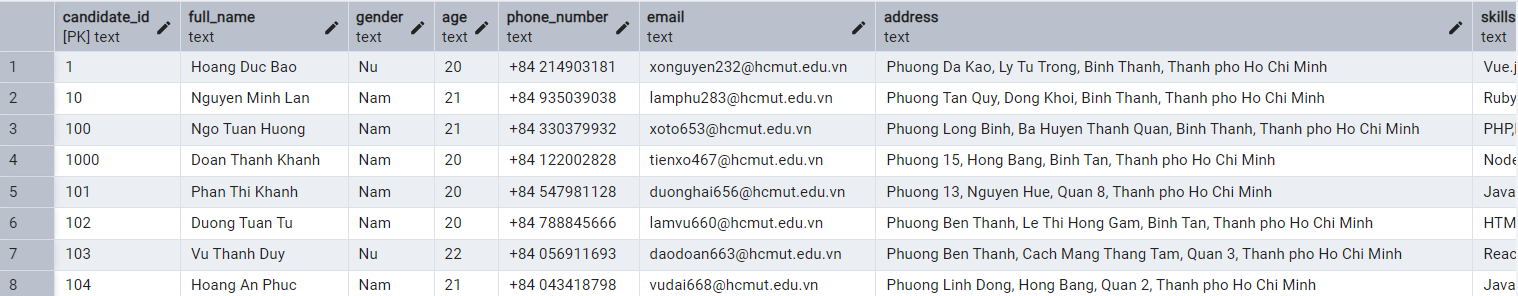
\includegraphics[width=\textwidth]{Image/2.1.2a.png}
        \caption{PostgreSQL lưu trữ dữ liệu dưới dạng bảng}
    \end{figure}
    \item Quản lý không gian lưu trữ: PostgreSQL sử dụng các cơ chế như TOAST (The Oversized-Attribute Storage Technique) để lưu trữ các giá trị lớn ngoài bảng chính.
    \begin{figure}[H]
        \centering
        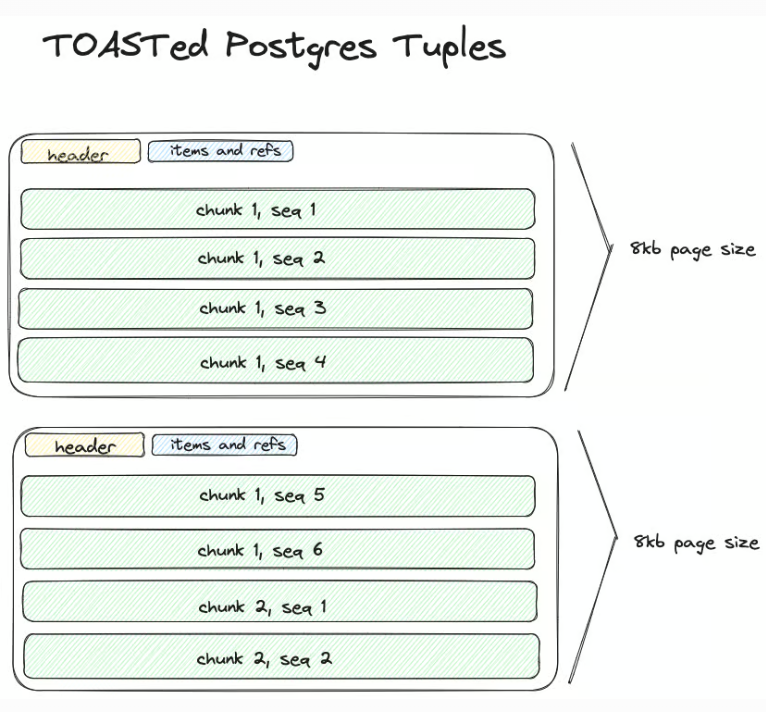
\includegraphics[width=0.9\textwidth]{Image/TOAST.png}
        \caption{Cơ chế TOAST trong PostgreSQL}
    \end{figure}
        \begin{itemize}
            \item Cách TOAST hoạt động
                \begin{itemize}
                    \item Khi một bài viết lớn được chèn vào bảng, PostgreSQL sẽ chia nhỏ nội dung của trường content thành các mảnh nhỏ hơn.
                    \item Các mảnh này được lưu trữ trong một bảng con do TOAST quản lý.
                    \item Bảng chính chỉ lưu trữ các tham chiếu tới các mảnh dữ liệu này.
                \end{itemize}
        \end{itemize}
    \item Truy vấn và tối ưu hóa: PostgreSQL cung cấp các công cụ tối ưu hóa truy vấn để đảm bảo hiệu suất cao khi truy xuất dữ liệu.
    \item Bảo mật và tính toàn vẹn: PostgreSQL hỗ trợ các chức năng bảo mật như kiểm soát quyền truy cập, mã hóa dữ liệu và kiểm tra tính toàn vẹn của dữ liệu.
\end{itemize}

\subsubsection{Data storage \& management trong MongoDB}
\indent MongoDB là một hệ quản trị cơ sở dữ liệu NoSQL và sử dụng mô hình tài liệu để lưu trữ dữ liệu. Các khía cạnh chính của data storage \& management trong MongoDB bao gồm:
\begin{itemize}
    \item Lưu trữ tài liệu: Dữ liệu được lưu trữ dưới dạng tài liệu JSON, cho phép lưu trữ dữ liệu không cấu trúc hoặc một phần cấu trúc. 
    \begin{figure}[H]
        \centering
        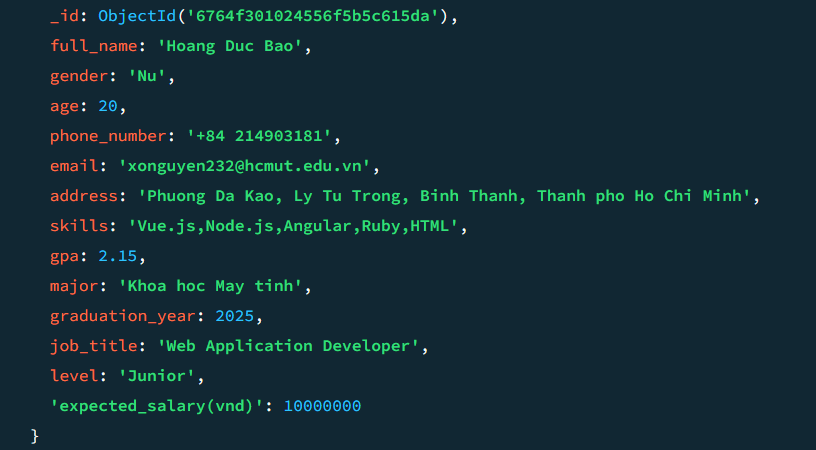
\includegraphics[width=0.9\textwidth]{Image/2.1.3a.png}
        \caption{Mongodb lưu trữ dữ liệu dưới tài liệu}
    \end{figure}
    \item Quản lý không gian lưu trữ: MongoDB sử dụng các cơ chế như sharding để phân chia dữ liệu lên nhiều máy chủ, giúp tăng khả năng mở rộng và hiệu suất.
    \begin{figure}[H]
        \centering
        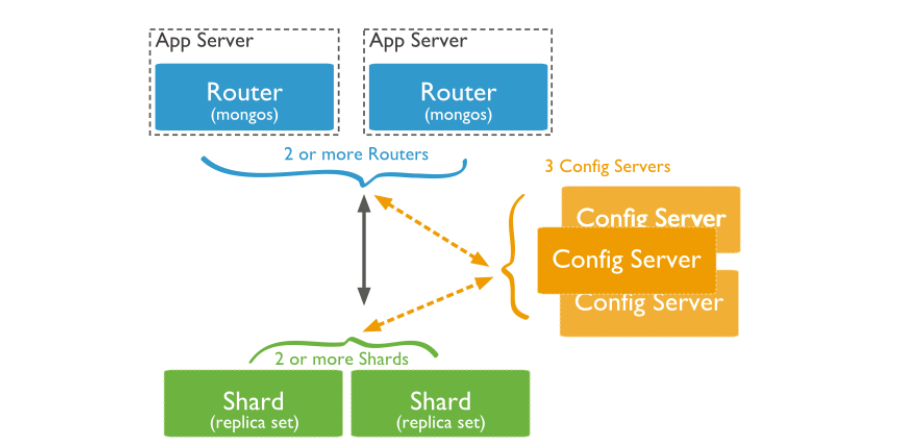
\includegraphics[width=0.9\textwidth]{Image/Sharding.png}
        \caption{Sharding trong MongoDB sử dụng Sharded Cluster}
    \end{figure}
    \item Truy vấn và tối ưu hóa: MongoDB cung cấp các công cụ truy vấn và tối ưu hóa để đảm bảo hiệu suất cao khi truy xuất dữ liệu.
    \item Bảo mật và tính toàn vẹn: MongoDB hỗ trợ các chức năng bảo mật như kiểm soát quyền truy cập, mã hóa dữ liệu và kiểm tra tính toàn vẹn của dữ liệu.
\end{itemize}

\subsubsection{So sánh}
\begin{itemize}
    \item Mô hình dữ liệu: PostgreSQL sử dụng mô hình bảng quan hệ, trong khi MongoDB sử dụng mô hình tài liệu JSON.
    \item Hiệu suất: PostgreSQL thường có hiệu suất tốt hơn cho các truy vấn phức tạp và các ứng dụng quan hệ, trong khi MongoDB có hiệu suất tốt hơn cho các ứng dụng với dữ liệu không cấu trúc hoặc một phần cấu trúc.
    \item Khả năng mở rộng: PostgreSQL hỗ trợ mở rộng qua các cơ chế như sharding và replication, nhưng MongoDB được thiết kế từ đầu để mở rộng theo mô hình scale-out.
    \item Tính linh hoạt: MongoDB cung cấp tính linh hoạt cao hơn cho các dữ liệu không cấu trúc, trong khi PostgreSQL cung cấp tính toàn vẹn và tính nhất quán cao hơn cho dữ liệu cấu trúc.
\end{itemize}

\begin{table}[H]
    \centering
    \begin{tabular}{|L{3.2cm}|L{5cm}|L{5cm}|} \hline 
         \textbf{Tiêu chí so sánh }&  \textbf{PostgreSQL}&  \textbf{MongoDB}\\ \hline 
         Mô hình dữ liệu &  Sử dụng các bảng quan hệ. & Sử dụng mô hình tài liệu JSON.\\ \hline 
         Hiệu suất &  Thích hợp cho các truy vấn phức tạp và ứng dụng quan hệ. & Hiệu suất tốt hơn cho dữ liệu phi cấu trúc và bán cấu trúc.\\ \hline 
         Khả năng mở rộng &  Hỗ trợ mở rộng qua cơ chế sharding và replication. &  Mở rộng theo mô hình scale-out.\\ \hline
         Tính linh hoạt &  Cung cấp tính toàn vẹn và tính nhất quán cho dữ liệu cấu trúc. &  Cung cấp tính linh hoạt cao hơn cho các dữ liệu không cấu trúc,.\\ \hline 
    \end{tabular}
    \caption{So sánh về Data storage \& management giữa PostgreSQL và MongoDB}
    \label{tab:data_storage&management}
\end{table}
\newpage
\subsection{Indexing}
\subsubsection{Lý thuyết}
\begin{itemize}
    \item Khái niệm:
        \begin{itemize}
            \item Indexing là một cấu trúc dữ liệu phụ trợ giúp tăng tốc việc tìm kiếm và truy cập dữ liệu trong cơ sở dữ liệu.
            \item Chỉ mục thường được xây dựng trên một hoặc nhiều trường, cung cấp đường dẫn truy cập hiệu quả đến các bản ghi trong bảng dữ liệu.
        \end{itemize}
    \item Các loại chỉ mục phổ biến: 
        \begin{itemize}
            \item Dựa trên tệp được sắp xếp: Single-level Ordered Indexes.
            \item Dựa trên các cấu trúc dữ liệu cây: Multilevel indexes, B+-trees.
            \item Các loại chỉ mục khác:
                \begin{itemize}
                    \item Hash indexes.
                    \item Bitmap indexes.
                    \item Function-based indexes.
                \end{itemize}
        \end{itemize}
    \item Single-level Ordered Indexes. Bao gồm: 
        \begin{itemize}
            \item Primary Indexes: 
                \begin{itemize}
                    \item Đặc điểm:
                        \begin{itemize}
                            \item Được tạo trên khóa chính (primary key) của bảng.
                            \item Chỉ mục này sắp xếp dữ liệu trong bảng theo thứ tự của khóa chính.
                            \item Mỗi bản ghi trong bảng có một giá trị khóa chính duy nhất.
                        \end{itemize}
                    \item Cấu trúc: Thường là dense index hoặc sparse index.
                        \begin{itemize}
                            \item Dense Index: Có một mục nhập chỉ mục cho mỗi bản ghi trong bảng.
                            \item Sparse Index: Chỉ lưu chỉ mục cho một số bản ghi nhất định (chỉ mục thưa).
                        \end{itemize}
                \end{itemize}
            \item Clustering Indexes:
                \begin{itemize}
                    \item Đặc điểm:
                        \begin{itemize}
                            \item Sắp xếp dữ liệu vật lý trong bảng theo một hoặc nhiều cột, gọi là khóa cluster.
                            \item Không nhất thiết phải là khóa chính, nhưng thường là một khóa duy nhất.
                            \item Một bảng chỉ có thể có một cluster index.
                        \end{itemize}
                    \item Cấu trúc: Clustered Index tạo ra một mối liên kết giữa thứ tự vật lý của các bản ghi và giá trị của cột được sắp xếp.
                \end{itemize}
            \item Secondary Indexes:
                \begin{itemize}
                    \item Đặc điểm:
                        \begin{itemize}
                            \item Được tạo trên bất kỳ cột nào không phải khóa chính hoặc khóa cluster.
                            \item Dùng để hỗ trợ truy vấn nhanh trên các cột khác không sắp xếp vật lý trong bảng.
                            \item Một bảng có thể có nhiều secondary index.
                        \end{itemize}
                    \item Cấu trúc: Thường là dense index, vì mỗi giá trị trong cột cần có một mục nhập trong chỉ mục.
                \end{itemize}
        \end{itemize}
\end{itemize}

\subsubsection{Indexing trong PostgreSQL}
\indent PostgreSQL hỗ trợ nhiều loại chỉ mục: 
\begin{itemize}
    \item B-Tree: Chỉ mục mặc định, phù hợp với truy vấn so sánh (=, <, >, BETWEEN).
        \begin{itemize}
            \item Cách khởi tạo:
\begin{lstlisting}[language=SQL]
CREATE INDEX idx_btree ON employees (age);
\end{lstlisting}
            \item Cách sử dụng:
\begin{lstlisting}[language=SQL]
SELECT * FROM employees WHERE age > 30;
\end{lstlisting}
        \end{itemize}
    \item Hash Index: Hash index được sử dụng chủ yếu cho các phép so sánh bằng (=). Tuy nhiên, nó ít được sử dụng hơn so với B-tree vì không hỗ trợ các phép so sánh khác như <, >.
        \begin{itemize}
            \item Cách khởi tạo:
\begin{lstlisting}[language=SQL]
CREATE INDEX idx_hash ON employees USING HASH (name);
\end{lstlisting}
            \item Cách sử dụng:
\begin{lstlisting}[language=SQL]
SELECT * FROM employees WHERE name = 'ABC';
\end{lstlisting}
        \end{itemize}
    \item GiST (Generalized Search Tree) là loại chỉ mục linh hoạt, cho phép chỉ mục trên các kiểu dữ liệu phức tạp như range, point, circle, text search, và hỗ trợ các toán tử: ($<<$,    \&<,   \&>,   $>>$,   $<<$|,   \&<|,   |\&>,   |$>>$,   @>,   <@,   $~=$,   \&\&).
        \begin{itemize}
            \item Cách khởi tạo:
\begin{lstlisting}[language=SQL]
CREATE INDEX idx_gist ON locations USING GiST (location);
\end{lstlisting}
            \item Cách sử dụng:
\begin{lstlisting}[language=SQL]
SELECT * FROM locations WHERE location @> 'POINT(1 1)';
\end{lstlisting}
        \end{itemize}
    \item SP-GiST (Space-partitioned Generalized Search Tree) là một loại chỉ mục hỗ trợ dữ liệu không gian và có thể sử dụng cho các loại dữ liệu như point, circle, và các loại dữ liệu không gian khác ($<<$,   $>>$,   $~$=,    <@,   $<<$|,   |$>>$).
        \begin{itemize}
            \item Cách khởi tạo:
\begin{lstlisting}[language=SQL]
CREATE INDEX idx_spgist ON locations USING SPGIST (location);
\end{lstlisting}
            \item Cách sử dụng:
\begin{lstlisting}[language=SQL]
SELECT * FROM locations WHERE location <-> 'POINT(1 1)' < 0.5;
\end{lstlisting}
        \end{itemize}
    \item GIN (Generalized Inverted Index) chủ yếu được sử dụng với các kiểu dữ liệu như array, jsonb, và tsvector. (<@,   @>,   $=$,   \&\&).
        \begin{itemize}
            \item Cách khởi tạo:
\begin{lstlisting}[language=SQL]
CREATE INDEX idx_gin ON documents USING GIN (content);
\end{lstlisting}
            \item Cách sử dụng:
\begin{lstlisting}[language=SQL]
SELECT * FROM documents WHERE content @@ to_tsquery('search_term');
\end{lstlisting}
        \end{itemize}
    \item BRIN (Block Range INdex)) thích hợp với các bảng rất lớn có dữ liệu theo thứ tự. BRIN không tạo chỉ mục cho từng giá trị mà tạo chỉ mục cho các block dữ liệu ($<,   <=,   =,   >=,   >\&$).
        \begin{itemize}
            \item Cách khởi tạo:
\begin{lstlisting}[language=SQL]
CREATE INDEX idx_brin ON measurements USING BRIN (timestamp);
\end{lstlisting}
            \item Cách sử dụng:
\begin{lstlisting}[language=SQL]
SELECT * FROM measurements WHERE timestamp > '2024-01-01';
\end{lstlisting}
        \end{itemize}
\end{itemize}
 
\subsubsection{Indexing trong MongoDB}
\indent MongoDB, với kiến trúc phi quan hệ, hỗ trợ các loại chỉ mục:
\begin{itemize}
    \item Single Field Index: Index trên một trường duy nhất. Đây là loại chỉ mục đơn giản và phổ biến nhất.
    \begin{figure}[H]
        \centering
        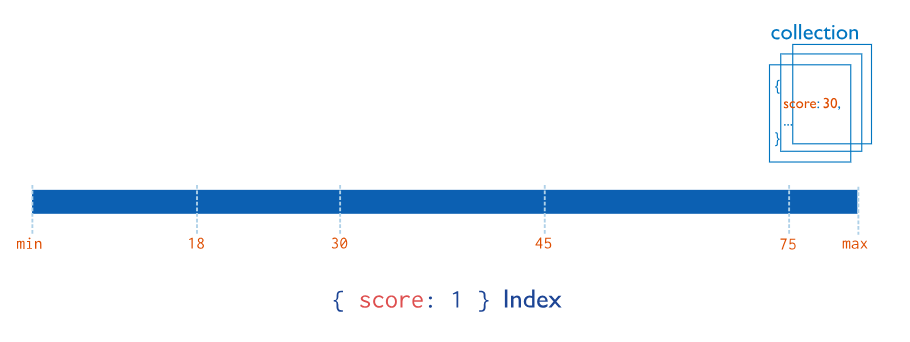
\includegraphics[width=\textwidth]{Image/2.2.3a.png}
        \caption{Single Field Index}
    \end{figure}
        \begin{itemize}
            \item Cách khởi tạo:
\begin{lstlisting}[language=SQL]
db.collection.createIndex({ fieldName: 1 }); 
\end{lstlisting}
            \item Cách sử dụng:
\begin{lstlisting}[language=inform]
db.users.createIndex({ age: 1 });
db.users.find({ age: { $gt: 25 } });
\end{lstlisting}
        \end{itemize}
    \item Compound Index: Index trên nhiều trường, phù hợp khi các truy vấn lọc dựa trên nhiều trường
    \begin{figure}[H]
        \centering
        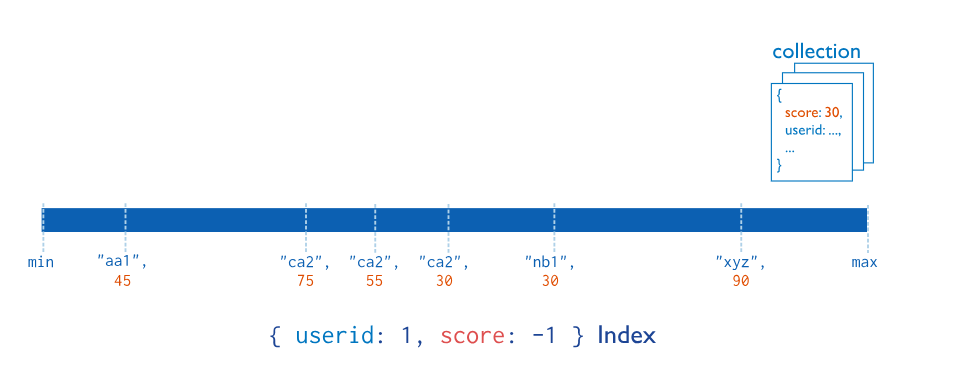
\includegraphics[width=\textwidth]{Image/2.2.3b.png}
        \caption{Compound Index}
    \end{figure}
        \begin{itemize}
            \item Cách khởi tạo:
\begin{lstlisting}[language=inform]
db.collection.createIndex({ field1: 1, field2: -1 });
\end{lstlisting}
            \item Cách sử dụng:
\begin{lstlisting}[language=inform]
db.users.createIndex({ age: 1, city: -1 });
db.users.find({ age: { $gte: 30 }, city: "New York" });
\end{lstlisting}
        \end{itemize}
    \item Multikey Index: Dành cho các trường chứa mảng. Mỗi giá trị trong mảng sẽ được lập chỉ mục.
    \begin{figure}[H]
        \centering
        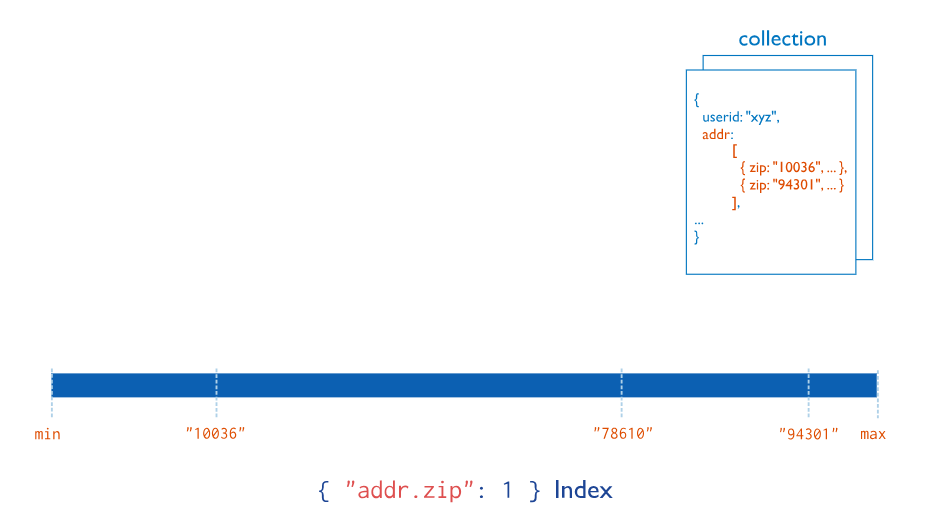
\includegraphics[width=\textwidth]{Image/2.2.3c.png}
        \caption{Multikey Index}
    \end{figure}
        \begin{itemize}
            \item Cách khởi tạo:
\begin{lstlisting}[language=inform]
db.collection.createIndex({ fieldName: 1 });
\end{lstlisting}
            \item Cách sử dụng:
\begin{lstlisting}[language=SQL]
db.products.createIndex({ tags: 1 });
db.products.find({ tags: "electronics" });
\end{lstlisting}
        \end{itemize}
    \item Geospatial Index: Dành cho dữ liệu không gian địa lý như tọa độ 2D hoặc 2DSphere.
        \begin{itemize}
            \item Cách khởi tạo:
\begin{lstlisting}[language=inform]
db.collection.createIndex({ location: "2dsphere" });
\end{lstlisting}
            \item Cách sử dụng:
\begin{lstlisting}[language=inform]
db.places.createIndex({ location: "2dsphere" });
db.places.find({
location: {
$near: {
$geometry: { type: "Point", coordinates: [40.7128, -74.0060] },
$maxDistance: 1000
}
}
});
\end{lstlisting}
        \end{itemize}
    \item  Wildcard Index: Index trên tất cả các trường hoặc một tập con trường, phù hợp với dữ liệu không có cấu trúc.
        \begin{itemize}
            \item Cách khởi tạo:
\begin{lstlisting}
db.collection.createIndex({ "$**": 1 });
\end{lstlisting}
            \item Cách sử dụng:
\begin{lstlisting}[language=inform]
db.logs.createIndex({ "$**": 1 });
db.logs.find({ "details.ip": "192.168.1.1" });
\end{lstlisting}
        \end{itemize}
    \item Hashed Index: Lập chỉ mục dựa trên giá trị băm của một trường, thường dùng để cân bằng tải truy vấn.
        \begin{itemize}
            \item Cách khởi tạo:
\begin{lstlisting}[language=SQL]
db.collection.createIndex({ fieldName: "hashed" });
\end{lstlisting}
            \item Cách sử dụng:
\begin{lstlisting}[language=SQL]
db.users.createIndex({ user_id: "hashed" });
db.users.find({ user_id: 12345 });
\end{lstlisting}
        \end{itemize}
\end{itemize}


\subsubsection{So sánh}
\begin{itemize}
    \item Đa dạng loại index: PostgreSQL hỗ trợ nhiều loại index phức tạp hơn phù hợp cho các truy vấn phức tạp và dữ liệu quan hệ, trong khi MongoDB tập trung vào các loại index phù hợp với dữ liệu không cấu trúc và dễ thay đổi.
    \item Ứng dụng và tối ưu hóa: PostgreSQL thường được sử dụng trong các ứng dụng đòi hỏi tính toàn vẹn, với các chỉ mục như GiST và GIN. Ngược lại, MongoDB phù hợp với các ứng dụng yêu cầu tốc độ và tính linh hoạt cao, với các chỉ mục như Multi-key và Geospatial.
    \item  Cấu trúc dữ liệu: PostgreSQL sử dụng các loại index để tối ưu hóa dữ liệu quan hệ, trong khi MongoDB sử dụng các loại index để tối ưu hóa dữ liệu tài liệu và các kiểu dữ liệu phi cấu trúc khác.
\end{itemize}
\begin{table}[H]
    \centering
    \begin{tabular}{|L{3.2cm}|L{5cm}|L{5cm}|} \hline 
         \textbf{Tiêu chí so sánh }&  \textbf{PostgreSQL}&  \textbf{MongoDB}\\ \hline 
         Sự tương thích &  Hỗ trợ nhiều toán tử, phép toán, thích hợp cho các truy vấn dữ liệu quan hệ phức tạp & Tập trung vào các loại index phù hợp với dữ liệu không cấu trúc và dễ thay đổi.\\ \hline 
         Ứng dụng và tối ưu hóa &  Đòi hỏi tính toàn vẹn của dữ liệu. & Thích hợp với dữ liệu thường xuyên thay đổi, tính linh hoạt cao, yêu cầu tốc độ truy xuất nhanh.\\ \hline 
         Cấu trúc dữ liệu &  Tối ưu hóa dữ liệu quan hệ. &  Tối ưu hóa dữ liệu tài liệu.\\ \hline
    \end{tabular}
    \caption{So sánh về Indexing giữa PostgreSQL và MongoDB}
    \label{tab:indexing}
\end{table}
\newpage






\subsection{Query processing}
\subsubsection{Lý thuyết}
\indent Query processing (Xử lý truy vấn) bao gồm các bước hệ thống cơ sở dữ liệu thực hiện để trả về kết quả mong muốn từ một truy vấn của người dùng. Quá trình này bao gồm nhiều bước từ việc phân tích, tối ưu hóa, thực thi và truy xuất kết quả. Các bước chính bao gồm:
\begin{itemize}
    \item Parsing (Phân tích cú pháp): Phân tích cú pháp truy vấn để đảm bảo nó đúng định dạng và cú pháp.
    \item Translation (Biên dịch): Chuyển truy vấn từ ngôn ngữ người dùng sang ngôn ngữ máy có thể hiểu.
    \item Optimization (Tối ưu hóa): Tìm kiếm các kế hoạch thực thi tối ưu để giảm thiểu chi phí và thời gian xử lý.
    \item Execution (Thực thi): Thực hiện kế hoạch truy vấn và truy xuất dữ liệu.
\end{itemize}
\begin{figure}[H]
    \centering
    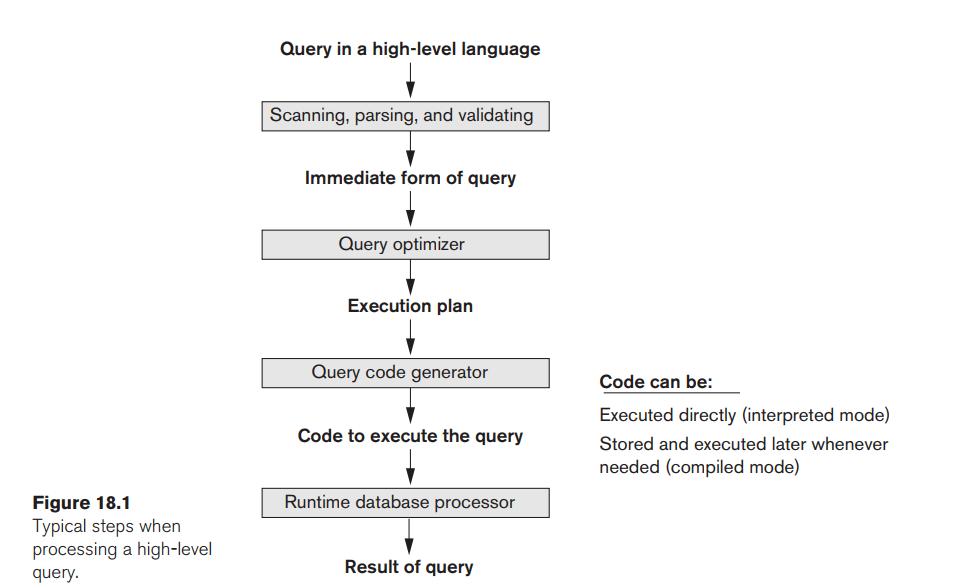
\includegraphics[width=\textwidth]{Image/2.3.1a.png}
    \caption{Các bước khi xử lý truy vấn cấp cao}
\end{figure}
\begin{itemize}
    \item Chi tiết mô tả các bước:
    \begin{itemize}
        \item Query in a high-level language (Truy vấn bằng ngôn ngữ bậc cao): Bắt đầu với một truy vấn được viết bằng ngôn ngữ bậc cao như SQL (trong PostgreSQL) hoặc MQL (trong MongoDB).
        \item Scanning, parsing, and validating (Quét, phân tích cú pháp và xác thực): Truy vấn này sau đó được quét, phân tích cú pháp để đảm bảo nó đúng về cú pháp và ngữ nghĩa.
        \item Immediate form of query (Dạng trung gian của truy vấn): Truy vấn sau khi được xác thực sẽ được chuyển thành dạng trung gian để dễ xử lý hơn.
        \item Query optimizer (Bộ tối ưu hóa truy vấn): Dạng trung gian của truy vấn được chuyển đến bộ tối ưu hóa truy vấn, nơi tạo ra kế hoạch thực thi tối ưu.
        \item Execution plan (Kế hoạch thực thi): Kế hoạch thực thi được tạo ra từ bộ tối ưu hóa.
        \item Query code generator (Bộ tạo mã truy vấn): Kế hoạch thực thi được chuyển đến bộ tạo mã truy vấn.
        \item Code to execute the query (Mã để thực thi truy vấn): Bộ tạo mã truy vấn sẽ tạo ra mã cần thiết để thực thi truy vấn.
        \item Runtime database processor (Bộ xử lý cơ sở dữ liệu runtime): Mã này được thực thi bởi bộ xử lý cơ sở dữ liệu runtime.
        \item Result of query (Kết quả của truy vấn): Cuối cùng, kết quả của truy vấn được trả về.
    \end{itemize}
\end{itemize}

\subsubsection{Query processing trong PostgreSQL}
\indent PostgreSQL sử dụng SQL làm ngôn ngữ truy vấn. Quy trình xử lý truy vấn trong PostgreSQL thường gồm ba bước chính:
\begin{itemize}
    \item Parsing: Phân tích cú pháp truy vấn SQL để tạo cây cú pháp (parse tree).
    \item Planning/Optimization: Sau khi cây cú pháp được tạo ra, PostgreSQL sẽ tiến hành Planning. Bước này sẽ giúp hệ thống quyết định cách thức thực thi truy vấn sao cho hiệu quả nhất. Hệ thống sẽ đánh giá và tạo ra một kế hoạch truy vấn (query plan) với các chiến lược tối ưu như:
        \begin{itemize}
            \item Join Optimization: Nếu có nhiều bảng tham gia vào truy vấn, PostgreSQL sẽ quyết định thứ tự join sao cho tối ưu nhất (sử dụng thuật toán join như Nested Loop, Merge Join, Hash Join).
            \item Index Optimization: Nếu có chỉ mục trên các cột, hệ thống sẽ chọn cách sử dụng các chỉ mục này để tối ưu hóa tìm kiếm thay vì phải quét toàn bộ bảng (full table scan).
            \item Heuristic Methods: Các phương pháp tối ưu hóa theo kinh nghiệm (heuristics) sẽ được áp dụng, như việc sử dụng các thuật toán sắp xếp hoặc kết hợp các chỉ mục.
        \end{itemize}
    \item Execution: Cuối cùng, kế hoạch truy vấn tối ưu sẽ được thực thi bởi executor của PostgreSQL. Executor sẽ thực hiện các phép toán theo kế hoạch đã tối ưu, trả về kết quả cuối cùng cho người dùng. Quá trình này có thể bao gồm quét bảng, áp dụng các phép toán join, và trả về kết quả.
\end{itemize}

\subsubsection{Query processing trong MongoDB}
\indent Mongodb sử dụng MongoDB Query Language (MQL) thay vì SQL. Quy trình xử lý truy vấn trong MongoDB bao gồm ba bước chính:
\begin{itemize}
    \item Parsing: Khi MongoDB nhận được một truy vấn, bước đầu tiên là Parsing, nơi MongoDB sẽ phân tích cú pháp của truy vấn MQL và tạo ra một cây cú pháp tương tự như trong PostgreSQL. Tuy nhiên, MongoDB sử dụng JSON-like documents (tài liệu kiểu JSON) thay vì bảng quan hệ, và truy vấn của MongoDB được cấu trúc dưới dạng các điều kiện như { field: value }.
    \item Planning/Optimization: Sau khi truy vấn được phân tích, MongoDB sẽ tạo ra một query plan. Quá trình tối ưu hóa truy vấn trong MongoDB chủ yếu dựa vào các chỉ mục có sẵn và cấu trúc tài liệu của MongoDB.
        \begin{itemize}
            \item Indexing: Nếu có chỉ mục trên trường age, MongoDB sẽ chọn sử dụng chỉ mục này để tìm kiếm các tài liệu thỏa mãn điều kiện age > 18, thay vì quét toàn bộ bộ sưu tập (collection).
            \item Query Optimization: MongoDB sẽ tối ưu hóa kế hoạch truy vấn để giảm thiểu số lượng tài liệu cần phải quét và cải thiện tốc độ truy vấn.
        \end{itemize}
    \item Execution: Sau khi tạo ra kế hoạch truy vấn tối ưu, MongoDB sẽ thực thi truy vấn đó bằng cách quét các tài liệu trong bộ sưu tập, áp dụng các chỉ mục (nếu có), và trả về kết quả.
\end{itemize}

\subsubsection{So sánh và kết luận}
\begin{itemize}
    \item Ngôn ngữ truy vấn: PostgreSQL sử dụng SQL, một ngôn ngữ truy vấn quan hệ tiêu chuẩn, trong khi MongoDB sử dụng MongoDB Query Language (MQL), phù hợp với dữ liệu không cấu trúc.
    \item Tối ưu hóa truy vấn: PostgreSQL áp dụng nhiều kỹ thuật tối ưu hóa phức tạp cho các truy vấn SQL, trong khi MongoDB tập trung vào tối ưu hóa dựa trên các chỉ mục và cấu trúc tài liệu.
    \item Thực thi truy vấn: PostgreSQL thực thi kế hoạch truy vấn trên các bảng quan hệ, trong khi MongoDB thực thi trên các tập hợp tài liệu, cho phép xử lý dữ liệu linh hoạt hơn.
\end{itemize}

\begin{table}[H]
    \centering
    \begin{tabular}{|L{3.2cm}|L{5cm}|L{5cm}|} \hline 
         \textbf{Tiêu chí so sánh }&  \textbf{PostgreSQL}&  \textbf{MongoDB}\\ \hline 
         Parsing &  Phân tích cú pháp SQL, tạo cây cú pháp. & Phân tích cú pháp MQL (JSON-like), tạo cây cú pháp.\\ \hline 
         Optimization &  Tối ưu hóa kế hoạch truy vấn sử dụng chỉ mục, thuật toán join, tối ưu hóa biểu thức. & Tối ưu hóa truy vấn dựa vào chỉ mục, cấu trúc tài liệu.\\ \hline 
         Execution &  Thực thi kế hoạch truy vấn, quét bảng hoặc sử dụng chỉ mục. &  Thực thi trên tập hợp tài liệu, xử lý dữ liệu linh hoạt.\\ \hline
    \end{tabular}
    \caption{So sánh về Query Processing PostgreSQL và MongoDB}
    \label{tab:query_processing}
\end{table}
\indent \textbf{Kết luận:}
\newpage

\subsection{Transaction}
\subsubsection{Lý thuyết}
\indent Trong Hệ Quản Trị Cơ Sở Dữ Liệu (DBMS), giao dịch là một khái niệm cốt lõi đại diện cho một tập hợp các thao tác logic được thực thi như một đơn vị duy nhất. Giao dịch đóng vai trò quan trọng trong việc xử lý các yêu cầu của người dùng nhằm truy cập và chỉnh sửa nội dung cơ sở dữ liệu, đảm bảo cơ sở dữ liệu luôn nhất quán và đáng tin cậy dù có nhiều thao tác hoặc gián đoạn xảy ra.\\

\indent Các thao tác chính của giao dịch:
\begin{enumerate}
    \item[1.] Read(X): Lấy giá trị X từ cơ sở dữ liệu và lưu vào bộ nhớ đệm. Ví dụ như kiểm tra số dư tài khoản.
    \item[2.] Write(X): Ghi giá trị từ bộ nhớ đệm vào cơ sở dữ liệu. Ví dụ như rút tiền từ tài khoản.
    \item[3.] Commit: Lưu các thay đổi của giao dịch vào cơ sở dữ liệu vĩnh viễn.
    \item[4.] Rollback: Hoàn tác giao dịch, đưa cơ sở dữ liệu về trạng thái trước đó khi giao dịch bị lỗi. 
\end{enumerate}

\indent Thuộc tính ACID:
\begin{enumerate}
    \item[1.] Atomicity: Giao dịch thực hiện toàn bộ hoặc không thực hiện gì.
    \item[2.] Consistency: Đảm bảo cơ sở dữ liệu nhất quán trước và sau giao dịch.
    \item[3.] Isolation: Các giao dịch không can thiệp lẫn nhau.
    \item[4.] Durability: Thay đổi được lưu vĩnh viễn sau khi giao dịch hoàn tất. 
\end{enumerate}
\subsubsection{Transaction trong PostgreSQL}
\indent Giao dịch là một khái niệm cốt lõi trong mọi hệ thống cơ sở dữ liệu. Điểm mấu chốt của một giao dịch là nó gói gọn nhiều bước thành một thao tác duy nhất với tính chất "tất cả hoặc không có gì". Các trạng thái trung gian giữa các bước không hiển thị đối với các giao dịch đồng thời khác, và nếu xảy ra sự cố ngăn giao dịch hoàn tất, thì không bước nào ảnh hưởng đến cơ sở dữ liệu.\\

PostgreSQL đảm bảo rằng các giao dịch tuân thủ đầy đủ các thuộc tính của mô hình ACID:
\begin{itemize}
    \item Tính toàn vẹn (Atomicity): Sử dụng cơ chế ghi nhật ký WAL (Write-Ahead Logging) để đảm bảo giao dịch được thực hiện hoàn toàn hoặc bị hủy bỏ hoàn toàn.
    \item Tính nhất quán (Consistency): Kiểm tra các ràng buộc dữ liệu (khóa chính, khóa ngoại, CHECK) để duy trì trạng thái hợp lệ của cơ sở dữ liệu sau giao dịch.
    \item Tính cách ly (Isolation): Hỗ trợ các mức cách ly như Read Committed, Repeatable Read, và Serializable để ngăn giao dịch bị ảnh hưởng bởi giao dịch khác.
    \item Tính bền vững (Durability): Cơ chế WAL đảm bảo thay đổi giao dịch được lưu vĩnh viễn, kể cả khi hệ thống gặp sự cố.
\end{itemize}

Trong quá trình thực thi, PostgreSQL đảm bảo trạng thái trung gian của giao dịch không hiển thị với các giao dịch đồng thời, tùy thuộc vào mức cách ly. Điều này giúp duy trì tính nhất quán và độ tin cậy của dữ liệu ngay cả khi xảy ra sự cố.\\

Ví dụ, bảng dữ liệu ứng viên gồm các cột như candidate\_id, full\_name, gender, age, phone\_number, email, address, skills, gpa, major, graduation\_year, job\_title, level, và expected\_salary(vnd). Trong một giao dịch, cần thực hiện các thao tác: giảm lương kỳ vọng của "Nguyen Van A" do đồng ý mức thấp hơn, thêm kỹ năng "Python" vào danh sách kỹ năng, và cập nhật chức danh công việc thành "Junior" nếu tốt nghiệp năm 2023. Giao dịch đảm bảo các thay đổi được thực hiện đồng nhất, không có trạng thái trung gian.\\

Mã SQL thực hiện giao dịch như sau: Đầu tiên, sử dụng lệnh UPDATE để giảm 2,000,000 VND từ mức lương kỳ vọng của ứng viên "Nguyen Van A". Tiếp theo, thêm kỹ năng "Python" vào danh sách kỹ năng hiện tại bằng hàm CONCAT. Cuối cùng, nếu ứng viên tốt nghiệp năm 2023, cập nhật chức danh công việc thành "Junior".
\begin{lstlisting}
-- 1. Giam muc luong ky vong cua ung vien "Nguyen Van A".
UPDATE candidates 
SET expected_salary = expected_salary - 2000000
WHERE candidate_id = 101 AND full_name = 'Nguyen Van A';

-- 2. Them ky nang "Python" vao danh sach ky nang cua ung vien.
UPDATE candidates 
SET skills = CONCAT(skills, ', Python')
WHERE candidate_id = 101 AND full_name = 'Nguyen Van A';

-- 3. Cap nhat chuc danh cong viec neu ung vien da tot nghiep nam 2023.
UPDATE candidates 
SET job_title = 'Junior Developer'
WHERE candidate_id = 101 AND graduation_year = 2023;
\end{lstlisting}

Giao dịch đảm bảo:
\begin{itemize}
    \item Tính nguyên tử (atomicity): Mọi thay đổi được thực hiện đồng thời hoặc không thay đổi nào được lưu nếu xảy ra lỗi. Ví dụ, nếu gặp lỗi khi thêm kỹ năng mới (như giá trị cột skills bị NULL), giao dịch sẽ tự động hủy, trả cơ sở dữ liệu về trạng thái ban đầu. Điều này loại trừ tình trạng dữ liệu không đồng bộ, như lương đã giảm nhưng kỹ năng mới chưa được thêm.
    \item Tính nhất quán (consistency): Mọi thay đổi đều dựa trên dữ liệu hợp lệ và các điều kiện đã đặt ra. Chẳng hạn, cập nhật chức danh chỉ thực hiện nếu ứng viên tốt nghiệp năm 2023, đảm bảo cơ sở dữ liệu chuyển từ trạng thái nhất quán này sang trạng thái nhất quán khác.
    \item Tính cách ly (isolation): Các giao dịch khác không nhìn thấy trạng thái trung gian của giao dịch đang thực hiện. Ví dụ, thay đổi về lương hoặc thêm kỹ năng mới chỉ hiển thị sau khi giao dịch hoàn tất với lệnh COMMIT. Điều này ngăn ngừa xung đột dữ liệu trong môi trường nhiều người dùng hoặc giao dịch đồng thời.
    \item Tính lâu dài (durability): Khi giao dịch hoàn tất, mọi thay đổi được ghi nhận vĩnh viễn. Ngay cả khi hệ thống gặp sự cố, dữ liệu như lương mới, kỹ năng mới và chức danh công việc vẫn không bị mất, nhờ được lưu trong nhật ký giao dịch (transaction log).
\end{itemize}

Giao dịch đảm bảo mọi thay đổi liên quan đến dữ liệu của ứng viên "Nguyen Van A" được thực hiện an toàn, nhất quán và không để lại trạng thái trung gian, giúp duy trì tính toàn vẹn dữ liệu và nâng cao độ tin cậy của hệ thống.\\

Trong PostgreSQL, giao dịch có thể được thiết lập bằng cách bao quanh các câu lệnh SQL của giao dịch bằng các lệnh BEGIN và COMMIT.\\
\begin{lstlisting}
BEGIN;
-- Giam muc luong ky vong cua ung vien "Nguyen Van A".
UPDATE candidates 
SET expected_salary = expected_salary - 2000000
WHERE candidate_id = 101 AND full_name = 'Nguyen Van A';
-- v.v
COMMIT;
\end{lstlisting}

Giao dịch bắt đầu bằng lệnh BEGIN và kết thúc bằng COMMIT. Các thay đổi (giảm lương, thêm kỹ năng, cập nhật chức danh) chỉ có hiệu lực sau khi COMMIT được thực thi, đảm bảo tất cả thao tác được thực hiện đồng thời. Nếu xảy ra lỗi (ví dụ, không thỏa mãn điều kiện), giao dịch sẽ bị hủy và cơ sở dữ liệu không bị ảnh hưởng.\\

PostgreSQL mặc định thực thi mỗi lệnh SQL trong một giao dịch ngầm và tự động COMMIT nếu lệnh thành công. Tuy nhiên, sử dụng BEGIN và COMMIT cho phép nhóm nhiều câu lệnh thành một giao dịch duy nhất, đảm bảo tính toàn vẹn dữ liệu.\\

Nếu trong quá trình giao dịch có vấn đề (như lương giảm quá thấp hoặc dữ liệu sai), bạn có thể hủy bỏ bằng lệnh ROLLBACK thay vì COMMIT, đảm bảo không có thay đổi nào được lưu vào cơ sở dữ liệu.\\

\begin{lstlisting}
BEGIN;
-- Giam muc luong ky vong cua ung vien "Nguyen Van A".
UPDATE candidates 
SET expected_salary = expected_salary - 2000000
WHERE candidate_id = 101 AND full_name = 'Nguyen Van A';
-- v.v
-- Neu phat hien su co, huy giao dich
ROLLBACK;
\end{lstlisting}

Với PostgreSQL, bạn có thể sử dụng savepoints để kiểm soát các câu lệnh trong giao dịch một cách chi tiết hơn. Savepoints cho phép bạn quay lại một điểm cụ thể trong giao dịch mà không làm ảnh hưởng đến các thay đổi đã thực hiện trước đó. Đây là một ví dụ về cách sử dụng savepoint trong một giao dịch:
\begin{lstlisting}
BEGIN;

-- Giam muc luong ky vong cua ung vien "Nguyen Van A"
UPDATE candidates 
SET expected_salary = expected_salary - 2000000
WHERE candidate_id = 101 AND full_name = 'Nguyen Van A';

-- Dat mot savepoint truoc khi cap nhat ky nang
SAVEPOINT my_savepoint;

-- Them ky nang "Python" vao danh sach ky nang cua ung vien
UPDATE candidates 
SET skills = CONCAT(skills, ', Python')
WHERE candidate_id = 101 AND full_name = 'Nguyen Van A';

-- Quay lai savepoint de loai bo thay doi ky nang
ROLLBACK TO my_savepoint;

-- Cap nhat chuc danh cong viec cua ung vien neu ho da tot nghiep nam 2023
UPDATE candidates 
SET job_title = 'Junior Developer'
WHERE candidate_id = 101 AND graduation_year = 2023;

-- Cam ket cac thay doi da thuc hien
COMMIT;
\end{lstlisting}

Trong ví dụ trên, giao dịch bắt đầu với lệnh BEGIN. Sau khi giảm mức lương kỳ vọng của ứng viên "Nguyen Van A", một điểm lưu được đặt bằng lệnh SAVEPOINT my\_savepoint trước khi thêm kỹ năng "Python". Khi phát hiện việc thêm kỹ năng không cần thiết, lệnh ROLLBACK TO my\_savepoint được sử dụng để loại bỏ thay đổi này nhưng vẫn giữ lại các thay đổi trước đó, như giảm mức lương kỳ vọng.\\

Cuối cùng, sau khi hoàn tất các thay đổi cần thiết (bao gồm cập nhật chức danh công việc), giao dịch kết thúc bằng lệnh COMMIT, đảm bảo tất cả thay đổi đã cam kết được ghi vào cơ sở dữ liệu.\\

Việc sử dụng savepoints cho phép kiểm soát linh hoạt trong giao dịch, giúp quay lại một điểm cụ thể mà không cần hủy toàn bộ giao dịch. Ngoài ra, ROLLBACK TO là giải pháp duy nhất để khôi phục một giao dịch đã bị lỗi, ngoại trừ việc hủy bỏ hoàn toàn và bắt đầu lại.\\

\subsubsection{Transaction trong MongoDB}
\indent Giao dịch MongoDB là tính năng cốt lõi đảm bảo tính toàn vẹn và độ tin cậy của dữ liệu thông qua ACID. Từ phiên bản 4.0, MongoDB hỗ trợ giao dịch ACID đa tài liệu, cho phép thực hiện các thao tác phức tạp trên nhiều tài liệu và bộ sưu tập trong một giao dịch duy nhất. Giao dịch này kết hợp các thao tác thành một đơn vị thống nhất, đảm bảo thực thi theo nguyên tắc "tất cả hoặc không có gì."\\

Điều này có nghĩa, nếu bất kỳ thao tác nào trong giao dịch thất bại, toàn bộ giao dịch sẽ bị hủy, và không thay đổi nào được áp dụng lên cơ sở dữ liệu. Cơ chế này bảo vệ tính toàn vẹn dữ liệu, duy trì trạng thái nhất quán ngay cả khi gặp sự cố, đồng thời ngăn ngừa lỗi hoặc dữ liệu không đầy đủ.\\

Thuật ngữ ACID đại diện cho bốn đặc tính trong quản lý giao dịch: Nguyên tử, Nhất quán, Cô lập, và Bền vững. Các giao dịch ACID trong MongoDB đảm bảo dữ liệu luôn toàn vẹn và nhất quán, cho phép thực hiện nhiều thao tác trên tài liệu, bộ sưu tập, cơ sở dữ liệu, hoặc phân đoạn như một đơn vị nguyên tử. MongoDB hỗ trợ giao dịch ACID đa tài liệu và phân tán, đảm bảo tính nguyên tử và nhất quán khi thực hiện thay đổi trên nhiều tài liệu hoặc trong hệ thống phân tán.\\

Giao dịch MongoDB xử lý các thao tác như một đơn vị nguyên tử, nghĩa là nếu tất cả thao tác thành công, giao dịch sẽ được hoàn tất. Ngược lại, nếu bất kỳ thao tác nào thất bại, mọi thay đổi sẽ bị hủy, đảm bảo hệ thống luôn ở trạng thái nhất quán.\\

Tính nhất quán được đảm bảo trong quá trình đồng bộ hóa giữa các tài liệu và bộ sưu tập. MongoDB hỗ trợ giao dịch đa tài liệu trên nhiều bộ sưu tập và cơ sở dữ liệu, giúp đơn giản hóa việc quản lý và duy trì tính toàn vẹn dữ liệu.\\

Giao dịch MongoDB rất hữu ích cho các ứng dụng yêu cầu trao đổi giá trị giữa các bên, như hệ thống ngân hàng, chuỗi cung ứng, hoặc nền tảng thương mại điện tử. Giao dịch ACID đảm bảo mọi bước trong quy trình, chẳng hạn chuyển tiền hoặc chuyển giao quyền sở hữu hàng hóa, được thực hiện chính xác và không xảy ra sự cố.\\

MongoDB cung cấp hai loại API để thực hiện giao dịch:
\begin{itemize}
    \item API cốt lõi: yêu cầu các lệnh gọi rõ ràng để bắt đầu và cam kết giao dịch.
    \item API gọi lại: tự động xử lý giao dịch, thực hiện các thao tác được chỉ định và cam kết hoặc hủy bỏ khi có lỗi.
\end{itemize}

Để tạo một phiên giao dịch, bạn có thể sử dụng MongoDB shell để bắt đầu giao dịch và thực hiện các thao tác trong đó. Nếu phiên giao dịch kéo dài hơn 60 giây sau khi gọi phương thức startTransaction(), MongoDB sẽ tự động hủy bỏ giao dịch để đảm bảo không có giao dịch nào kéo dài quá lâu và ảnh hưởng đến hiệu suất hệ thống.\\


Giao dịch trong cơ sở dữ liệu MongoDB đảm bảo tính hợp lệ của dữ liệu bất chấp các sự gián đoạn và lỗi thông qua bốn thuộc tính cốt lõi: tính nguyên tử, tính nhất quán, tính cô lập và tính bền vững.
\begin{itemize}
    \item Tính nguyên tử: Đảm bảo giao dịch là một khối thống nhất. Nếu bất kỳ thao tác nào thất bại, toàn bộ giao dịch sẽ bị hủy để ngăn dữ liệu không nhất quán.
    \item Tính nhất quán: Cơ sở dữ liệu luôn duy trì trạng thái hợp lệ. Giao dịch vi phạm nguyên tắc nhất quán sẽ bị hủy bỏ.
    \item Tính cô lập: Giao dịch đồng thời không ảnh hưởng lẫn nhau. Trạng thái trung gian không hiển thị cho giao dịch khác cho đến khi hoàn tất.
    \item Tính bền vững: Sau khi hoàn tất, mọi thay đổi được lưu vĩnh viễn, ngay cả khi hệ thống gặp sự cố.
\end{itemize}

Mặc dù giao dịch trong MongoDB mang lại nhiều lợi ích, nhưng cũng có một số nhược điểm cần được lưu ý. Dưới đây là một số yếu tố nhược điểm khi sử dụng giao dịch trong MongoDB:
\begin{itemize}
    \item Tác động đến hiệu suất: Giao dịch có thể làm giảm hiệu suất hệ thống, đặc biệt khi ghi dữ liệu lớn, do yêu cầu khóa và đồng bộ hóa giữa các tài liệu và bộ sưu tập, gây thêm chi phí xử lý.
    \item Độ phức tạp: Quản lý giao dịch trong MongoDB có thể phức tạp, đặc biệt với các nhà phát triển chưa quen với hệ thống phân tán. Việc xử lý giao dịch trên nhiều tài liệu và phân đoạn đòi hỏi hiểu biết sâu, khiến việc triển khai trở nên thách thức hơn.
\end{itemize}

Ví dụ ta có một bộ dữ liệu MongoDB chứa thông tin về các ứng viên, với các trường như candidate\_id, full\_name, gender, age, phone\_number, email, address, skills, gpa, major, graduation\_year, job\_title, level, và expected\_salary.
\begin{lstlisting}
    from pymongo import MongoClient

client = MongoClient("mongodb://localhost:27017")
database = client["your_database"]

with client.start_session() as session:
    session.start_transaction()
    try:
        # Vi du ve viec them mot ung vien moi
        database.candidates.insert_one({
            "candidate_id": "1001",
            "full_name": "Nguyen Van A",
            "gender": "Nam",
            "age": 31,
            "phone_number": "0123456789",
            "email": "nguyen.vana@example.com",
            "address": "123 Duong Vi du, Thanh pho, Viet Nam",
            "skills": ["Python", "Hoc may", "Phan tich du lieu"],
            "gpa": 3.8,
            "major": "Khoa hoc may tinh",
            "graduation_year": 2022,
            "job_title": "Ky su phan mem",
            "level": "Junior",
            "expected_salary(vnd)": 20000000
        }, session=session)

        # Vi du ve viec cap nhat thong tin mot ung vien da co
        database.candidates.update_one(
            {"candidate_id": "1001"},
            {"$set": {
                "full_name": "Nguyen Van B",
                "expected_salary(vnd)": 25000000
            }},
            session=session
        )

        # Xac nhan giao dich
        session.commit_transaction()
    except Exception as e:
        # Huy giao dich neu co loi
        print("Da xay ra loi:", e)
        session.abort_transaction()

\end{lstlisting}

Đoạn mã Python sử dụng thư viện pymongo để kết nối và thao tác với MongoDB. Mã thực hiện giao dịch nhằm đảm bảo tính toàn vẹn dữ liệu: thêm một tài liệu mới vào bộ sưu tập candidates và cập nhật thông tin ứng viên hiện có. Nếu giao dịch thành công, các thay đổi được cam kết (commit); nếu xảy ra lỗi, giao dịch sẽ bị hủy (abort) để đảm bảo dữ liệu không bị ảnh hưởng sai lệch.
\begin{itemize}
    \item start\_session(): Phương thức trong PyMongo để bắt đầu một phiên làm việc mới, cho phép thực hiện các thao tác đọc/ghi dữ liệu trong phạm vi của một giao dịch.
    \item start\_transaction(): Khởi tạo giao dịch mới trong phiên làm việc, đảm bảo tuân thủ các đặc tính ACID. Nếu có lỗi, giao dịch có thể bị hủy và các thay đổi sẽ được hoàn lại.
    \item commit\_transaction(): Xác nhận tất cả thay đổi trong giao dịch, làm chúng trở thành vĩnh viễn và hiển thị cho các phiên khác.
    \item abort\_transaction(): Hủy giao dịch khi xảy ra lỗi, hoàn lại toàn bộ thay đổi để giữ nguyên trạng thái dữ liệu ban đầu.
    \item withTransaction: Công cụ tiện ích của MongoDB driver, tự động quản lý giao dịch (bắt đầu, cam kết hoặc hủy) bằng cách bao bọc các thao tác trong một hàm, đơn giản hóa mã lệnh.
\end{itemize}


Nếu giao dịch thành công, một tài liệu mới sẽ được thêm vào bộ sưu tập candidates với đầy đủ thông tin như candidate\_id, full\_name, gender, age, phone\_number, email, address, skills, gpa, major, graduation\_year, job\_title, level, và expected\_salary (vnd). Sau đó, tài liệu này sẽ được cập nhật với tên mới là "Nguyen Van B" và mức lương kỳ vọng thay đổi thành 25,000,000 VND. Ngược lại, nếu xảy ra lỗi như lỗi kết nối hoặc thao tác không hợp lệ, giao dịch sẽ bị hủy để giữ nguyên trạng thái dữ liệu, và thông báo lỗi sẽ được in ra màn hình dưới dạng: "Đã xảy ra lỗi: <thông tin lỗi>".
\subsubsection{So sánh và kết luận}
\begin{itemize}
    \item Mô hình dữ liệu: PostgreSQL sử dụng mô hình quan hệ, trong đó dữ liệu được tổ chức trong bảng với schema cố định, trong khi MongoDB sử dụng mô hình NoSQL, lưu trữ dữ liệu dưới dạng tài liệu và hỗ trợ schema linh hoạt.
    \item Hỗ trợ ACID: PostgreSQL hỗ trợ đầy đủ các thuộc tính ACID trên mọi giao dịch, bao gồm giao dịch liên quan đến nhiều bảng, trong khi MongoDB chỉ hỗ trợ ACID trên các giao dịch nhiều tài liệu từ phiên bản 4.0.
    \item Giao dịch nhiều bảng: PostgreSQL được tối ưu hóa để xử lý các giao dịch giữa các bảng có mối quan hệ chặt chẽ, trong khi MongoDB cũng hỗ trợ giao dịch nhiều tài liệu nhưng hiệu năng có thể bị giảm khi giao dịch phức tạp.
    \item Isolation Levels: PostgreSQL cung cấp đầy đủ các mức độ cô lập giao dịch như Read Uncommitted, Read Committed, Repeatable Read, và Serializable, trong khi MongoDB chủ yếu hỗ trợ mức cô lập tương tự Read Committed.
    \item Concurrency Control: PostgreSQL sử dụng cơ chế MVCC (Multi-Version Concurrency Control) để quản lý truy cập đồng thời hiệu quả, trong khi MongoDB áp dụng snapshot isolation qua engine WiredTiger.
    \item Hiệu năng: PostgreSQL có hiệu năng vượt trội khi xử lý giao dịch phức tạp và liên quan đến nhiều bảng, trong khi MongoDB hoạt động tốt hơn với các giao dịch đơn giản trên tài liệu.
    \item Hạn chế giao dịch: PostgreSQL không gặp bất kỳ hạn chế nào trong việc thực hiện giao dịch đa bảng hoặc phức tạp, trong khi MongoDB giới hạn các giao dịch ACID trong một cluster hoặc replica set.
    \item Quản lý dữ liệu: PostgreSQL yêu cầu dữ liệu phải tuân theo schema chặt chẽ, điều này lý tưởng cho các hệ thống phức tạp, trong khi MongoDB linh hoạt hơn, phù hợp với các ứng dụng cần thay đổi cấu trúc dữ liệu nhanh chóng.
\end{itemize}
\begin{table}[H]
    \centering
    \begin{tabular}{|L{3.2cm}|L{5.05cm}|L{5.05cm}|} \hline 
         \textbf{Tiêu chí so sánh }&  \textbf{PostgreSQL}&  \textbf{MongoDB}\\ \hline 
         Mô hình dữ liệu & Quan hệ (dữ liệu trong bảng, schema cố định) & NoSQL (dữ liệu dạng tài liệu, schema linh hoạt)\\ \hline 
         Hỗ trợ ACID & Hoàn toàn hỗ trợ ACID trên từng giao dịch, bao gồm cả các bảng liên quan. & Hỗ trợ ACID trên các giao dịch nhiều tài liệu kể từ MongoDB 4.0.\\ \hline
         Giao dịch nhiều bảng & Hoàn toàn hỗ trợ, được tối ưu cho các bảng có quan hệ chặt chẽ. & Hỗ trợ, nhưng hiệu năng có thể giảm nếu giao dịch liên quan nhiều tài liệu.\\ \hline
         Isolation Levels & Đầy đủ các mức độ cô lập: Read Uncommitted, Read Committed, Repeatable Read, Serializable. & Cơ bản hỗ trợ mức độ cô lập giống Read Committed (không hỗ trợ tất cả các mức).\\ \hline
         Concurrency Control & MVCC (Multi-Version Concurrency Control) giúp quản lý truy cập đồng thời hiệu quả. & WiredTiger engine sử dụng cơ chế snapshot isolation.\\ \hline
         Performance (hiệu năng) & Giao dịch phức tạp, nhiều bảng thường nhanh hơn vì được thiết kế tối ưu cho RDBMS. & Hiệu năng tốt với giao dịch đơn giản trên tài liệu. Giao dịch phức tạp có thể chậm hơn.\\ \hline
         Hạn chế giao dịch & Không có hạn chế đặc biệt với giao dịch đa bảng hoặc phức tạp. & Giao dịch ACID chỉ hoạt động trong một cụm shard (cluster) hoặc replica set.\\ \hline
         Quản lý dữ liệu & Dữ liệu phải tuân theo schema chặt chẽ, cần thiết cho giao dịch phức tạp. & Dữ liệu linh hoạt, thích hợp cho các ứng dụng cần thay đổi nhanh chóng.\\ \hline
    \end{tabular}
    \caption{So sánh về Transaction giữa PostgreSQL và MongoDB}
    \label{tab:transaction}
\end{table}
\indent \textbf{Kết luận:}
\newpage
\subsection{Concurrency control}
\subsubsection{Lý thuyết}
\indent Kiểm soát đồng thời là một khái niệm cốt lõi trong hệ quản trị cơ sở dữ liệu (DBMS), nhằm đảm bảo rằng nhiều quy trình hoặc người dùng có thể thao tác dữ liệu cùng lúc mà không gây ra sự không nhất quán. Chức năng này quản lý cách các giao dịch được thực thi xen kẽ với nhau.\\

Để đảm bảo tính nhất quán của dữ liệu, hệ quản trị cơ sở dữ liệu sử dụng nhiều phương pháp điều khiển đồng thời khác nhau. Một số phương pháp phổ biến bao gồm:
\begin{itemize}
    \item Khóa (Locking): Sử dụng các loại khóa như khóa đọc (read lock) hoặc khóa ghi (write lock) để hạn chế quyền truy cập vào dữ liệu, ngăn chặn các giao dịch khác can thiệp khi một giao dịch đang thao tác.
    \item Đóng dấu thời gian (Timestamping): Các giao dịch được gắn nhãn thời gian và quyền truy cập dữ liệu được kiểm soát dựa trên thứ tự thời gian này.
    \item Kiểm soát lạc quan (Optimistic Control): Giả định rằng xung đột sẽ hiếm xảy ra và chỉ kiểm tra tính nhất quán khi giao dịch chuẩn bị hoàn tất.
    \item Hủy và khôi phục (Rollback and Recovery): Nếu phát hiện lỗi hoặc xung đột, giao dịch sẽ bị hủy bỏ và hệ thống khôi phục về trạng thái trước đó.
    \item Lập lịch giao dịch (Transaction Scheduling): Điều phối thứ tự thực hiện các giao dịch để tránh các tình huống xung đột.
\end{itemize}
\subsubsection{Concurrency control trong PostgreSQL}
\indent
PostgreSQL sử dụng mô hình đa phiên bản (MVCC) để quản lý quyền truy cập đồng thời vào dữ liệu, đảm bảo tính nhất quán và cách ly giao dịch. MVCC cho phép mỗi câu lệnh SQL truy cập một phiên bản dữ liệu (snapshot) tại thời điểm nhất định, bất kể trạng thái hiện tại của dữ liệu. Nhờ vậy, các giao dịch đồng thời không gây ra xung đột hoặc dữ liệu không nhất quán, đồng thời giảm thiểu tranh chấp khóa và nâng cao hiệu suất trong môi trường đa người dùng.\\

Ưu điểm lớn nhất của mô hình MVCC so với phương pháp khóa là khả năng tách biệt giữa đọc và ghi, giúp việc đọc không cản trở ghi và ngược lại. PostgreSQL duy trì tính năng này ngay cả ở mức cách ly giao dịch cao nhất nhờ cơ chế Serializable Snapshot Isolation (SSI) tiên tiến.\\

PostgreSQL hỗ trợ khóa cấp bảng và dòng cho các ứng dụng không cần cách ly giao dịch cao nhưng muốn quản lý xung đột cụ thể. Tuy nhiên, MVCC thường mang lại hiệu suất tốt hơn. Ngoài ra, cơ chế khóa tư vấn cho phép ứng dụng sử dụng các khóa độc lập với giao dịch.\\

Chuẩn SQL định nghĩa bốn mức cách ly giao dịch, với Serializable là mức cao nhất, đảm bảo kết quả tương đương khi thực hiện tuần tự. Ba mức còn lại ngăn các hiện tượng không nhất quán khác nhau trong các giao dịch đồng thời.
\begin{itemize}
    \item Đọc bẩn (dirty read): Giao dịch đọc dữ liệu từ giao dịch khác chưa cam kết ghi.
    \item Đọc không lặp lại (nonrepeatable read): Giao dịch đọc lại dữ liệu đã đọc trước đó và phát hiện dữ liệu đã thay đổi bởi giao dịch khác đã cam kết.
    \item Đọc bóng ma (phantom read): Giao dịch thực thi lại truy vấn và phát hiện tập hợp các hàng thỏa mãn điều kiện đã thay đổi do giao dịch vừa cam kết.
    \item Bất thường trong tuần tự hóa (serialization anomaly): Kết quả cam kết thành công của nhóm giao dịch không nhất quán với bất kỳ thứ tự thực hiện tuần tự nào của các giao dịch đó.
\end{itemize}
\begin{enumerate}
    \item Read Uncommitted Isolation Level
    
    \hspace{1cm}Cấp độ cô lập Read Uncommitted là một trong bốn cấp độ cô lập được chuẩn SQL định nghĩa, nhưng PostgreSQL không hỗ trợ trực tiếp. Thay vào đó, PostgreSQL đảm bảo rằng mọi truy vấn, kể cả ở cấp độ thấp nhất, chỉ có thể truy cập dữ liệu đã được cam kết.

    \hspace{1cm}Đặc điểm chính của Read Uncommitted:
    \begin{itemize}
        \item Đọc dữ liệu chưa cam kết: Cho phép các giao dịch đọc dữ liệu tạm thời từ những giao dịch chưa cam kết, dẫn đến nguy cơ "dirty read".
        \item Hiệu năng cao nhưng không đảm bảo tính nhất quán: Thích hợp trong trường hợp ưu tiên hiệu suất, nhưng không đảm bảo dữ liệu chính xác hoặc toàn vẹn.
        \item Không khả dụng trong PostgreSQL: PostgreSQL không cung cấp cấp độ này vì chính sách đảm bảo tính toàn vẹn dữ liệu.
    \end{itemize}

    \hspace{1cm}Nếu cần mô phỏng Read Uncommitted trong PostgreSQL, bạn có thể sử dụng các cài đặt đặc biệt như vô hiệu hóa kiểm tra MVCC hoặc áp dụng các phương pháp khác. Tuy nhiên, điều này không được khuyến khích vì có thể ảnh hưởng đến tính toàn vẹn dữ liệu.
    \item Read Committed Isolation Level

    \hspace{1cm}Mức độ cách ly Read Committed là chế độ mặc định trong PostgreSQL, trong đó:
    \begin{itemize}
        \item Truy vấn SELECT: Chỉ nhìn thấy dữ liệu đã được cam kết tại thời điểm truy vấn bắt đầu. Nó không hiển thị thay đổi chưa cam kết hoặc thay đổi từ các giao dịch đồng thời trong quá trình truy vấn. Tuy nhiên, truy vấn vẫn thấy các thay đổi chưa cam kết trong phạm vi giao dịch của chính nó.
        \item Cơ chế của UPDATE, DELETE, SELECT FOR UPDATE, SELECT FOR SHARE: Chỉ thao tác trên các hàng đã cam kết tại thời điểm lệnh bắt đầu. Nếu các hàng này bị khóa hoặc thay đổi bởi giao dịch đồng thời, lệnh sẽ đợi giao dịch kia hoàn tất và sau đó kiểm tra lại điều kiện tìm kiếm (WHERE) trước khi thực hiện.
        \item Lệnh INSERT với ON CONFLICT:
        \begin{itemize}
            \item Với ON CONFLICT DO UPDATE, lệnh có thể cập nhật các hàng đang được giao dịch khác thay đổi, mặc dù các thay đổi đó không hiển thị ngay.
            \item Với ON CONFLICT DO NOTHING, nếu giao dịch khác thay đổi dữ liệu gây xung đột, lệnh sẽ bỏ qua mà không thực thi.
        \end{itemize}
        \item Lệnh MERGE: Kết hợp INSERT, UPDATE, DELETE, đánh giá lại điều kiện trên các phiên bản cập nhật của hàng. Tuy nhiên, nếu xung đột xảy ra (như vi phạm duy nhất), lệnh không tự khởi động lại mà có thể gây lỗi, dẫn đến nguy cơ mất tính nhất quán.
    \end{itemize}

    \hspace{1cm}Mặc dù Read Committed mang lại hiệu suất cao và phù hợp với các thao tác đơn giản, nhưng nó không đủ mạnh cho các ứng dụng yêu cầu tính nhất quán cao. Ví dụ, khi hai giao dịch đồng thời cập nhật cùng một hàng, các thao tác có thể thấy dữ liệu khác nhau, gây ra kết quả không đồng nhất. Trong các trường hợp phức tạp hơn, việc sử dụng các mức độ cách ly cao hơn như Repeatable Read hoặc Serializable là cần thiết để đảm bảo tính chính xác và toàn vẹn dữ liệu.
    \item Repeatable Read Isolation Level

    \hspace{1cm}Mức độ cách ly Repeatable Read trong PostgreSQL đảm bảo mỗi giao dịch chỉ nhìn thấy dữ liệu đã được cam kết trước khi giao dịch bắt đầu. Trong quá trình thực thi, giao dịch không nhìn thấy dữ liệu chưa cam kết hoặc các thay đổi từ các giao dịch đồng thời. Tuy nhiên, các thay đổi do chính giao dịch thực hiện vẫn có thể được nhìn thấy, ngay cả khi chưa cam kết.

    \hspace{1cm}So với Read Committed, nơi mỗi truy vấn thấy dữ liệu cam kết tại thời điểm truy vấn bắt đầu, Repeatable Read sử dụng một snapshot cố định của cơ sở dữ liệu tại thời điểm giao dịch khởi đầu. Điều này đảm bảo các truy vấn SELECT trong cùng một giao dịch luôn thấy cùng một dữ liệu, bất kể thay đổi từ các giao dịch đồng thời.

    \hspace{1cm}Một số đặc điểm quan trọng của Repeatable Read:
    \begin{itemize}
        \item Các lệnh như UPDATE, DELETE, MERGE, SELECT FOR UPDATE và SELECT FOR SHARE chỉ tác động đến dữ liệu đã được cam kết tại thời điểm giao dịch bắt đầu.
        \item Nếu một hàng bị thay đổi hoặc khóa bởi giao dịch khác, giao dịch hiện tại phải chờ giao dịch đó hoàn thành. Nếu giao dịch kia cam kết thay đổi, giao dịch hiện tại sẽ bị hủy và báo lỗi "could not serialize access due to concurrent update".
    \end{itemize}

    \hspace{1cm} Repeatable Read bảo vệ tính ổn định của dữ liệu trong giao dịch, ngăn chặn hiện tượng dirty reads và non-repeatable reads. Dù vậy, nó không đảm bảo tuyệt đối tính tuần tự giữa các giao dịch. Ứng dụng cần xử lý lỗi tuần tự hóa và có cơ chế thử lại giao dịch khi cần thiết.
    \item Serializable Isolation Level

    \hspace{1cm}Mức độ cách ly Serializable là mức cao nhất và nghiêm ngặt nhất trong PostgreSQL, đảm bảo rằng các giao dịch được thực thi như thể chúng diễn ra tuần tự, từng giao dịch một. Điều này giúp duy trì tính toàn vẹn và nhất quán của dữ liệu, bất kể số lượng giao dịch đồng thời. Tuy nhiên, nếu không thể xác định được một thứ tự thực thi tuần tự hợp lệ, các giao dịch sẽ bị hủy, và ứng dụng cần chuẩn bị để thử lại khi gặp lỗi tuần tự hóa.

    \hspace{1cm}Serializable không chỉ ngăn chặn các hiện tượng như dirty reads, non-repeatable reads, và phantom reads mà còn phát hiện và ngăn các tình huống khiến giao dịch không thể tuân theo một thứ tự tuần tự. Hệ thống sẽ tự động hủy bỏ giao dịch nếu phát hiện xung đột không thể giải quyết. Điều này đảm bảo rằng mọi giao dịch đồng thời đều tương thích với một thứ tự tuần tự hợp lệ.

    \hspace{1cm}Để đạt được điều này, PostgreSQL sử dụng kỹ thuật Predicate Locking. Hệ thống theo dõi các phụ thuộc giữa các giao dịch đồng thời thông qua các khóa theo điều kiện. Mặc dù không gây ra deadlock, kỹ thuật này có thể làm tăng chi phí tài nguyên và ảnh hưởng đến hiệu suất, đặc biệt trong môi trường có nhiều giao dịch đồng thời.

    \hspace{1cm}Serializable đảm bảo tính nhất quán tuyệt đối, nhưng các giao dịch đồng thời vẫn có thể gặp lỗi tuần tự hóa. Một ví dụ phổ biến là vi phạm ràng buộc duy nhất, ngay cả khi dữ liệu đã được kiểm tra trước khi chèn. Điều này xảy ra khi nhiều giao dịch đồng thời tranh giành tài nguyên. Để giảm thiểu xung đột, ứng dụng cần thực hiện các kiểm tra kỹ lưỡng và sẵn sàng thử lại giao dịch khi gặp lỗi.

    \hspace{1cm}Để sử dụng Serializable hiệu quả:
    \begin{itemize}
        \item Giảm thiểu xung đột: Hạn chế số lượng kết nối đồng thời và giảm độ phức tạp của giao dịch. Tránh sử dụng các khóa như SELECT FOR UPDATE hoặc SELECT FOR SHARE khi không cần thiết.
        \item Cấu hình hệ thống: Tinh chỉnh các tham số như max\_pred\_locks\_per\_transaction, max\_pred\_locks\_per\_relation, và max\_pred\_locks\_per\_page để giảm khả năng xảy ra lỗi tuần tự hóa.
        \item Chuẩn bị xử lý lỗi: Ứng dụng nên tự động xử lý và thử lại giao dịch nếu bị hủy do lỗi tuần tự hóa.
    \end{itemize}

    \hspace{1cm}Serializable là mức cách ly mạnh mẽ và lý tưởng cho các ứng dụng yêu cầu tính nhất quán và chính xác cao. Tuy nhiên, để sử dụng hiệu quả, cần quản lý chặt chẽ tài nguyên, tối ưu hiệu suất hệ thống, và chuẩn bị chiến lược xử lý lỗi tuần tự hóa.
\end{enumerate}

PostgreSQL cung cấp nhiều chế độ khóa giúp kiểm soát truy cập đồng thời vào dữ liệu trong các bảng. Các chế độ này được sử dụng khi cơ chế MVCC không đáp ứng đủ yêu cầu. Hầu hết các lệnh PostgreSQL tự động áp dụng khóa phù hợp để ngăn ngừa việc xóa hoặc sửa đổi bảng một cách không tương thích. Ví dụ, lệnh TRUNCATE yêu cầu khóa ACCESS EXCLUSIVE trên bảng để thực hiện thao tác, ngăn không cho các hoạt động khác xảy ra đồng thời.
\begin{enumerate}
    \item Khóa cấp độ bảng

    \hspace{1cm}PostgreSQL sử dụng các chế độ khóa cấp bảng để đảm bảo tính nhất quán của dữ liệu trong giao dịch. Các khóa này có thể áp dụng tự động hoặc qua lệnh LOCK. Mặc dù tên gọi có thể gây nhầm lẫn, tất cả đều là khóa cấp bảng. Sự khác biệt chính giữa các chế độ khóa là mức độ xung đột giữa chúng. Một giao dịch không thể giữ nhiều khóa xung đột trên cùng một bảng cùng lúc, nhưng có thể giữ các khóa xung đột đối với chính nó.

    \hspace{1cm}Các chế độ khóa trong PostgreSQL có thể được phân loại như sau:
    \begin{itemize}
        \item ACCESS SHARE: Khóa cơ bản, chỉ xung đột với ACCESS EXCLUSIVE. Dùng cho các lệnh SELECT không thay đổi dữ liệu.
        \item ROW SHARE: Xung đột với EXCLUSIVE và ACCESS EXCLUSIVE. Dùng cho SELECT với các tùy chọn như FOR UPDATE hoặc FOR SHARE, khi cần khóa bảng để cập nhật dữ liệu.
        \item ROW EXCLUSIVE: Xung đột với SHARE, SHARE ROW EXCLUSIVE, EXCLUSIVE, và ACCESS EXCLUSIVE. Dùng cho các lệnh UPDATE, DELETE, INSERT, và MERGE.
        \item SHARE UPDATE EXCLUSIVE: Xung đột với SHARE, ROW EXCLUSIVE, EXCLUSIVE, và ACCESS EXCLUSIVE. Dùng cho VACUUM, ANALYZE, CREATE INDEX CONCURRENTLY và một số lệnh ALTER INDEX.
        \item SHARE: Xung đột với ROW EXCLUSIVE, SHARE UPDATE EXCLUSIVE, và EXCLUSIVE. Dùng cho CREATE INDEX để ngăn thay đổi dữ liệu trong khi thực hiện thao tác đọc.
        \item SHARE ROW EXCLUSIVE: Xung đột với ROW EXCLUSIVE, SHARE, EXCLUSIVE, và ACCESS EXCLUSIVE. Chỉ cho phép một giao dịch giữ khóa này tại một thời điểm, dùng khi tạo TRIGGER hoặc thực hiện ALTER TABLE.
        \item EXCLUSIVE: Xung đột với hầu hết các khóa khác, chỉ cho phép giữ khóa ACCESS SHARE đồng thời. Dùng cho REFRESH MATERIALIZED VIEW CONCURRENTLY.
        \item ACCESS EXCLUSIVE: Khóa mạnh nhất, xung đột với tất cả các khóa khác. Dùng cho các lệnh như DROP TABLE, TRUNCATE, REINDEX, CLUSTER, và VACUUM FULL.
    \end{itemize}

    \hspace{1cm}Các khóa này sẽ được giữ cho đến khi giao dịch kết thúc. Nếu khóa được lấy sau khi thiết lập điểm lưu (savepoint), nó sẽ bị giải phóng nếu giao dịch bị rollback về điểm lưu đó, đảm bảo tính nhất quán của hệ thống.
    \item Khóa cấp hàng

    \hspace{1cm}PostgreSQL hỗ trợ các chế độ khóa cấp hàng để đảm bảo tính toàn vẹn dữ liệu trong giao dịch, không ảnh hưởng đến việc truy vấn nhưng ngăn chặn các thay đổi đối với các hàng đang bị khóa cho đến khi giao dịch hoàn tất. Các chế độ khóa cấp hàng bao gồm:
    \begin{itemize}
        \item FOR UPDATE: Khóa các hàng trong lệnh SELECT như thể chúng sẽ được cập nhật, ngăn các giao dịch khác thực hiện các thao tác như UPDATE, DELETE, SELECT FOR UPDATE, SELECT FOR NO KEY UPDATE, SELECT FOR SHARE, hoặc SELECT FOR KEY SHARE cho đến khi giao dịch hiện tại hoàn tất. Trong các giao dịch với mức độ cô lập REPEATABLE READ hoặc SERIALIZABLE, nếu hàng bị thay đổi từ khi giao dịch bắt đầu, một lỗi sẽ xảy ra.
        \item FOR NO KEY UPDATE: Tương tự như FOR UPDATE nhưng khóa yếu hơn, không ngăn chặn các lệnh SELECT FOR KEY SHARE trên cùng một hàng. Dùng khi không cần khóa toàn bộ hàng một cách nghiêm ngặt như FOR UPDATE.
        \item FOR SHARE: Khóa chia sẻ, ngăn các giao dịch khác thực hiện UPDATE, DELETE, SELECT FOR UPDATE, hoặc SELECT FOR NO KEY UPDATE, nhưng cho phép SELECT FOR SHARE hoặc SELECT FOR KEY SHARE.
        \item FOR KEY SHARE: Khóa yếu hơn FOR SHARE, chỉ ngăn các thao tác DELETE hoặc UPDATE thay đổi giá trị khóa, không ảnh hưởng đến các cột khác hoặc các lệnh SELECT FOR NO KEY UPDATE, SELECT FOR SHARE, SELECT FOR KEY SHARE.
    \end{itemize}

    \hspace{1cm}PostgreSQL không lưu trữ thông tin về các hàng đã sửa đổi trong bộ nhớ, do đó không giới hạn số lượng hàng có thể bị khóa. Tuy nhiên, khóa một hàng có thể dẫn đến ghi đĩa, ví dụ khi SELECT FOR UPDATE sửa đổi các hàng để đánh dấu chúng là bị khóa. Các khóa cấp hàng sẽ được giải phóng khi giao dịch kết thúc hoặc trong quá trình phục hồi điểm lưu.
    \item Khóa cấp trang

    \hspace{1cm}Ngoài các khóa cấp bảng và khóa cấp hàng, PostgreSQL còn sử dụng khóa chia sẻ và khóa độc quyền cấp trang để quản lý quyền truy cập đọc/ghi vào các trang bảng trong bộ đệm dùng chung. Những khóa này sẽ được giải phóng ngay sau khi một hàng được truy xuất hoặc cập nhật. Mặc dù các nhà phát triển ứng dụng thường không cần phải tương tác trực tiếp với các khóa cấp trang, nhưng chúng được nhắc đến ở đây để đảm bảo tính đầy đủ của hệ thống quản lý khóa trong PostgreSQL.
    \item Bế tắc

    \hspace{1cm}Việc sử dụng khóa rõ ràng có thể dẫn đến tình trạng bế tắc khi hai hoặc nhiều giao dịch giữ các khóa mà giao dịch kia cần. Ví dụ, nếu giao dịch 1 giữ khóa độc quyền trên bảng A và muốn khóa bảng B, trong khi giao dịch 2 giữ khóa độc quyền trên bảng B và muốn khóa bảng A, cả hai giao dịch sẽ bị chặn. PostgreSQL sẽ tự động phát hiện và giải quyết tình trạng bế tắc bằng cách hủy một giao dịch, cho phép giao dịch còn lại tiếp tục. Tuy nhiên, không thể dự đoán giao dịch nào bị hủy, vì vậy không nên dựa vào điều này.

    \hspace{1cm}Tình trạng bế tắc không chỉ xảy ra với khóa rõ ràng mà còn có thể phát sinh từ khóa cấp hàng. Khi hai giao dịch đồng thời sửa đổi cùng một bảng, nếu một giao dịch giữ khóa cấp hàng trên một hàng và giao dịch kia cố gắng cập nhật hàng đó, tình trạng bế tắc có thể xảy ra. PostgreSQL sẽ phát hiện và giải quyết bằng cách hủy một giao dịch.

    \hspace{1cm}Để phòng tránh bế tắc, một biện pháp hiệu quả là đảm bảo các ứng dụng sử dụng cơ sở dữ liệu lấy khóa theo thứ tự nhất quán. Nếu cả hai giao dịch đều khóa các hàng theo cùng một thứ tự, bế tắc sẽ không xảy ra. Ngoài ra, các giao dịch nên giữ khóa với mức độ hạn chế nhất có thể để giảm thiểu khả năng xung đột. Nếu không thể tránh được, tình trạng bế tắc có thể được xử lý thông qua cơ chế thử lại các giao dịch bị hủy.

    \hspace{1cm}Để tránh bế tắc, các ứng dụng nên đảm bảo việc lấy khóa theo thứ tự nhất quán. Nếu các giao dịch khóa hàng theo cùng thứ tự, bế tắc sẽ không xảy ra. Các giao dịch cũng nên giữ khóa trong phạm vi tối thiểu để giảm xung đột. Nếu bế tắc không thể tránh, có thể xử lý qua cơ chế thử lại các giao dịch bị hủy. Nếu không phát hiện được bế tắc, giao dịch có thể chờ vô hạn để lấy khóa. Vì vậy, ứng dụng nên tránh giữ giao dịch mở quá lâu, đặc biệt khi chờ người dùng nhập dữ liệu.
    \item Khóa tư vấn

    \hspace{1cm}PostgreSQL cung cấp cơ chế khóa tư vấn, cho phép ứng dụng tạo ra các khóa theo nhu cầu và không bị hệ thống buộc phải sử dụng. Những khóa này mang tính tùy chọn và có thể hữu ích cho các chiến lược khóa không phù hợp với mô hình MVCC (Multi-Version Concurrency Control). Một ví dụ điển hình là việc sử dụng khóa tư vấn để mô phỏng các chiến lược khóa bi quan, thường thấy trong các hệ thống quản lý dữ liệu dạng "flat file". Khóa tư vấn giúp tránh làm đầy bảng dữ liệu, nhanh chóng và tự động được dọn dẹp vào cuối phiên.

    \hspace{1cm}Trong PostgreSQL, khóa tư vấn có thể được lấy ở hai mức độ: cấp độ phiên và cấp độ giao dịch. Khóa cấp độ phiên sẽ được giữ cho đến khi được giải phóng hoặc phiên kết thúc, không phụ thuộc vào trạng thái giao dịch. Các khóa cấp độ giao dịch, tương tự như khóa thông thường, sẽ tự động được giải phóng khi giao dịch kết thúc. Hành vi của khóa cấp độ phiên thường thuận tiện hơn trong các trường hợp sử dụng ngắn hạn, vì chúng không yêu cầu thao tác mở khóa rõ ràng.

    \hspace{1cm}Khóa tư vấn có thể được theo dõi thông qua chế độ xem hệ thống pg\_locks, giống như các khóa thông thường. Tuy nhiên, vì cả khóa tư vấn và khóa thông thường đều được lưu trong bộ nhớ chia sẻ, nên cần chú ý đến việc không làm cạn kiệt bộ nhớ này, để tránh việc máy chủ không thể cấp thêm khóa. Giới hạn này được xác định bởi các tham số cấu hình max\_locks\_per\_transaction và max\_connections, và có thể dẫn đến số lượng khóa tư vấn bị giới hạn từ hàng chục đến hàng trăm nghìn, tùy vào cấu hình máy chủ.

    \hspace{1cm}Khi sử dụng khóa tư vấn, đặc biệt trong các truy vấn có liên quan đến thứ tự hoặc mệnh đề LIMIT, cần cẩn thận với thứ tự đánh giá các biểu thức SQL. Một số trường hợp có thể dẫn đến việc khóa không được giải phóng như mong đợi nếu LIMIT không được áp dụng trước khi khóa được lấy, dẫn đến tình trạng khóa treo lơ lửng mà không được giải phóng cho đến khi kết thúc phiên.
\end{enumerate}


Trong khi giao dịch sử dụng chế độ xem dữ liệu ổn định như cơ chế Đọc lặp lại, có một vấn đề tinh tế liên quan đến việc sử dụng ảnh chụp nhanh MVCC để kiểm tra tính nhất quán của dữ liệu: xung đột đọc/ghi. Cụ thể, nếu một giao dịch ghi dữ liệu và một giao dịch khác đồng thời cố gắng đọc cùng dữ liệu, giao dịch đọc sẽ không thể thấy những thay đổi của giao dịch ghi. Điều này có thể khiến giao dịch đọc “nhìn thấy” dữ liệu như thể nó đã được ghi trước khi giao dịch ghi bắt đầu hoặc cam kết. Dù vậy, vấn đề thực sự phát sinh khi giao dịch đọc đồng thời ghi lại dữ liệu mà nó đã đọc, tạo ra tình huống một giao dịch có thể dường như thực thi trước các giao dịch khác mặc dù cam kết sau. Khi điều này xảy ra, một chu kỳ có thể xuất hiện trong biểu đồ thực thi giao dịch, làm cho các kiểm tra tính toàn vẹn không thể hoạt động chính xác nếu thiếu sự hỗ trợ đặc biệt.
\begin{enumerate}
    \item Thực thi tính nhất quán với các giao dịch có thể tuần tự hóa

    \hspace{1cm}Khi mức cô lập giao dịch Serializable được áp dụng cho tất cả các thao tác ghi và các lần đọc cần chế độ xem dữ liệu nhất quán, không cần phải thực hiện thêm bất kỳ biện pháp nào để đảm bảo tính nhất quán. Phần mềm từ các môi trường khác được thiết kế để sử dụng giao dịch serializable nhằm duy trì tính nhất quán sẽ "hoạt động" theo cách này trong PostgreSQL.
    
    \hspace{1cm}Việc sử dụng kỹ thuật này giúp giảm bớt gánh nặng cho các lập trình viên ứng dụng, bởi nếu phần mềm ứng dụng sử dụng một khuôn khổ tự động thử lại các giao dịch bị lỗi tuần tự hóa, các vấn đề này sẽ được khắc phục mà không cần sự can thiệp thủ công. Việc đặt default\_transaction\_isolation thành serializable có thể là một giải pháp hợp lý. Đồng thời, cần đảm bảo rằng không có mức cô lập giao dịch nào khác được sử dụng, vô tình hoặc cố ý, nhằm phá hoại các kiểm tra tính toàn vẹn, thông qua việc kiểm tra mức cô lập giao dịch trong các kích hoạt.
    \item Thực thi tính nhất quán với Khóa chặn rõ ràng

    \hspace{1cm}Khi thực hiện các lệnh ghi không tuần tự hóa, để đảm bảo tính hợp lệ và bảo vệ hàng khỏi các bản cập nhật đồng thời, cần sử dụng các câu lệnh như SELECT FOR UPDATE, SELECT FOR SHARE, hoặc LOCK TABLE. Trong đó, SELECT FOR UPDATE và SELECT FOR SHARE chỉ khóa các hàng được trả về, ngăn chặn cập nhật đồng thời, còn LOCK TABLE khóa toàn bộ bảng. Đây là điều cần lưu ý khi chuyển ứng dụng từ môi trường khác sang PostgreSQL.

    \hspace{1cm}Một lưu ý quan trọng là SELECT FOR UPDATE không ngăn giao dịch đồng thời cập nhật hoặc xóa hàng đã chọn trừ khi thực hiện thao tác UPDATE. Câu lệnh này chỉ tạm thời chặn các giao dịch khác khỏi thao tác trên hàng bị khóa, nhưng khi giao dịch giữ khóa xác nhận, giao dịch bị chặn vẫn có thể tiếp tục với xung đột trừ khi có thao tác UPDATE thực sự.
    
    \hspace{1cm}Kiểm tra tính hợp lệ toàn cục trong môi trường MVCC không tuần tự hóa đòi hỏi cẩn thận. Ví dụ, khi kiểm tra tổng các khoản tín dụng và ghi nợ trong các bảng đang cập nhật đồng thời, so sánh hai câu lệnh SELECT sum(...) sẽ không chính xác trong chế độ Đọc đã cam kết. Cả hai phép tính nên được thực hiện trong một giao dịch đọc lặp lại để đảm bảo tính chính xác về các giao dịch đã cam kết trước khi giao dịch đọc bắt đầu.
    
    \hspace{1cm}Trong trường hợp này, khóa tất cả các bảng cần thiết để kiểm tra sẽ đảm bảo tính chính xác. Việc sử dụng chế độ khóa SHARE (hoặc cao hơn) đảm bảo không có thay đổi chưa cam kết nào trong bảng bị khóa, ngoại trừ thay đổi của giao dịch hiện tại.
    
    \hspace{1cm}Nếu dựa vào khóa để ngăn ngừa thay đổi đồng thời, cần chắc chắn rằng khóa đã được lấy trước khi thực hiện truy vấn. Ảnh chụp nhanh trong giao dịch đọc lặp lại bị đóng băng khi truy vấn hoặc sửa đổi dữ liệu đầu tiên được thực hiện, vì vậy cần lấy khóa trước khi ảnh chụp nhanh bị ghi nhận.
\end{enumerate}

PostgreSQL cung cấp khả năng truy cập dữ liệu bảng mà không bị chặn đối với các thao tác đọc/ghi, tuy nhiên, không phải tất cả các phương thức truy cập chỉ mục đều hỗ trợ tính năng này. Cụ thể, các loại chỉ mục khác nhau được xử lý như sau:
\begin{itemize}
    \item Chỉ mục B-tree, GiST và SP-GiST: Các chỉ mục này sử dụng khóa chia sẻ và khóa độc quyền cấp trang trong thời gian ngắn cho các thao tác đọc/ghi, và được giải phóng ngay sau khi mỗi hàng chỉ mục được truy xuất hoặc chèn. Các phương pháp này đảm bảo khả năng đồng thời cao mà không xảy ra deadlock.
    \item CChỉ mục Hash: Với chỉ mục hash, khóa chia sẻ và khóa độc quyền được áp dụng ở cấp bucket hash cho các thao tác đọc/ghi, và giải phóng sau khi toàn bộ bucket được xử lý. Mặc dù khóa cấp bucket cung cấp khả năng đồng thời tốt hơn so với khóa cấp chỉ mục, nhưng do thời gian giữ khóa lâu hơn, deadlock vẫn có thể xảy ra.
    \item Chỉ mục GIN: Chỉ mục GIN sử dụng các khóa chia sẻ và khóa độc quyền cấp trang trong thời gian ngắn cho các thao tác đọc/ghi. Các khóa này được giải phóng ngay sau khi mỗi hàng chỉ mục được truy xuất hoặc chèn. Tuy nhiên, việc chèn một giá trị vào chỉ mục GIN thường dẫn đến nhiều lần chèn khóa chỉ mục cho mỗi giá trị, do đó, mỗi lần chèn có thể yêu cầu thực hiện nhiều thao tác hơn.
\end{itemize}

Tính đến hiện tại, chỉ mục B-tree là lựa chọn tối ưu cho các ứng dụng cần hỗ trợ đồng thời, nhờ vào khả năng cung cấp hiệu suất cao và tính linh hoạt vượt trội so với chỉ mục hash. Do đó, B-tree là loại chỉ mục được khuyến nghị cho các ứng dụng đồng thời yêu cầu lập chỉ mục dữ liệu vô hướng. Đối với dữ liệu không vô hướng, các loại chỉ mục như GiST, SP-GiST hoặc GIN nên được ưu tiên sử dụng.
\subsubsection{Concurrency control trong MongoDB}
\indent Kiểm soát đồng thời trong MongoDB đảm bảo các thao tác diễn ra đồng thời nhưng vẫn duy trì tính chính xác và nhất quán. Thay vì sử dụng phương pháp bi quan như các hệ thống khóa, MongoDB áp dụng phương pháp lạc quan với WiredTiger, nơi việc kiểm tra xung đột chỉ xảy ra khi cần thiết. Nếu phát hiện xung đột ghi, một thao tác sẽ bị hủy và thực hiện lại. Khi hai thao tác đồng thời, ít nhất một là ghi, gây xung đột với các ràng buộc, MongoDB sẽ tự động hủy bỏ và thử lại thao tác ghi xung đột.\\

MongoDB sử dụng cơ chế khóa để đảm bảo tính chính xác của dữ liệu khi thực hiện các thao tác đồng thời. Hệ thống khóa của MongoDB bao gồm khóa đọc, khóa ghi và khóa ý định, giúp quản lý hiệu quả các truy cập đồng thời mà vẫn duy trì tính toàn vẹn dữ liệu.
\begin{enumerate}
    \item Khóa đọc: Khóa chia sẻ trên một tài nguyên như bộ sưu tập hoặc cơ sở dữ liệu, khi được giữ, cho phép người đọc đồng thời nhưng không cho phép người ghi. 
    \item Khóa ghi: Khóa độc quyền được áp dụng trên một tài nguyên, chẳng hạn như bộ sưu tập hoặc cơ sở dữ liệu, khi một tiến trình thực hiện thao tác ghi. Loại khóa này đảm bảo rằng không có tiến trình nào khác có thể ghi hoặc đọc từ tài nguyên đó cho đến khi tiến trình hiện tại hoàn tất, nhằm duy trì tính toàn vẹn dữ liệu.
    \item Khóa ý định: Khóa trên tài nguyên chỉ rõ rằng người sở hữu khóa sẽ thực hiện các thao tác đọc (với mục đích chia sẻ) hoặc ghi (với mục đích không chia sẻ) trên tài nguyên, đồng thời áp dụng cơ chế kiểm soát đồng thời chi tiết hơn so với khóa ý định. Trong khi đó, khóa ý định cho phép cả người đọc và người ghi có thể truy cập đồng thời vào tài nguyên đó.
\end{enumerate}

MongoDB, thông qua công cụ lưu trữ WiredTiger, áp dụng phương pháp kiểm soát đồng thời lạc quan. Thay vì ngăn chặn các thao tác từ trước, WiredTiger cho phép chúng thực hiện song song và chỉ kiểm tra xung đột sau khi các thao tác đã hoàn thành. Phương pháp này giúp tăng hiệu suất trong các môi trường có tần suất xung đột thấp.
\begin{enumerate}
    \item Hoạt động và hạn chế
    \begin{itemize}
        \item Không thể ghim tài liệu vào bộ nhớ đệm của WiredTiger.
        \item WiredTiger không phân biệt bộ nhớ đệm cho thao tác đọc và ghi.
        \item Khối lượng công việc ghi lớn có thể ảnh hưởng đến hiệu suất, nhưng WiredTiger ưu tiên lưu trữ đệm chỉ mục trong các trường hợp này.
        \item Bộ nhớ đệm của WiredTiger được phân bổ cho toàn bộ phiên bản mongod, không phân bổ ở cấp độ cơ sở dữ liệu hoặc bộ sưu tập.
    \end{itemize}
    \item Giao dịch (Đọc và Ghi) Đồng thời
    \begin{itemize}
        \item Thuật toán điều chỉnh động: Từ phiên bản 7.0, MongoDB tự động điều chỉnh số lượng giao dịch đồng thời (vé đọc và ghi) để tối ưu hóa thông lượng khi quá tải cụm.
        \item Giới hạn vé: Số lượng vé đọc và ghi tối đa là 128 và có thể khác nhau giữa các nút. Mỗi nút có số lượng vé đọc và ghi bằng nhau.
        \item Cấu hình: Sử dụng storageEngineConcurrentReadTransactions và storageEngineConcurrentWriteTransactions để chỉ định số lượng tối đa.
        \item Tắt thuật toán: Để tắt thuật toán, yêu cầu hỗ trợ từ Kỹ sư dịch vụ kỹ thuật MongoDB.
        \item Xem số lượng giao dịch: Dùng lệnh serverStatus và queues.execution để kiểm tra số lượng giao dịch.
        \item Quá tải cụm: Giá trị availablein thấp không chỉ ra quá tải; số lượng phiếu xếp hàng mới là dấu hiệu quá tải.
    \end{itemize}
    \item Tính đồng thời ở cấp độ tài liệu
    \begin{itemize}
        \item Kiểm soát đồng thời cấp tài liệu: WiredTiger sử dụng kiểm soát đồng thời cấp tài liệu cho các hoạt động ghi, cho phép nhiều máy khách sửa đổi tài liệu khác nhau cùng lúc trong một bộ sưu tập.
        \item Kiểm soát đồng thời lạc quan: Hầu hết các hoạt động đọc và ghi sử dụng kiểm soát đồng thời lạc quan, với khóa ý định ở cấp độ toàn cục, cơ sở dữ liệu và bộ sưu tập.
        \item Xung đột ghi: Khi có xung đột giữa hai hoạt động, một hoạt động sẽ gặp xung đột ghi và MongoDB sẽ thử lại tự động.
        \item Khóa toàn phiên bản: Một số hoạt động toàn cục yêu cầu khóa "toàn phiên bản" toàn cục, thường là các hoạt động ngắn hạn liên quan đến nhiều cơ sở dữ liệu.
        \item Khóa cơ sở dữ liệu độc quyền: Một số hoạt động như renameCollection yêu cầu khóa cơ sở dữ liệu độc quyền trong một số trường hợp nhất định.
    \end{itemize}
    \item Ảnh chụp nhanh và Điểm kiểm tra
    \begin{itemize}
        \item MVCC: WiredTiger sử dụng MultiVersion Concurrency Control (MVCC) để cung cấp ảnh chụp nhanh dữ liệu, đảm bảo chế độ xem nhất quán.
        \item Điểm kiểm tra: Dữ liệu ảnh chụp nhanh được ghi vào đĩa và điểm kiểm tra giúp đảm bảo tính nhất quán và khôi phục khi có sự cố.
        \item Tạo điểm kiểm tra: MongoDB cấu hình để tạo điểm kiểm tra mỗi 60 giây. Điểm kiểm tra cũ vẫn hợp lệ cho đến khi điểm mới được ghi và cập nhật.
        \item Khôi phục: Nếu có lỗi khi ghi điểm kiểm tra, MongoDB có thể khôi phục từ điểm kiểm tra cuối cùng hợp lệ.
        \item Giải phóng dữ liệu cũ: Khi điểm kiểm tra mới có thể truy cập, WiredTiger giải phóng các trang từ điểm kiểm tra cũ.
        \item Lưu giữ lịch sử ảnh chụp: Dùng tham số minSnapshotHistoryWindowInSeconds để chỉ định thời gian lưu giữ ảnh chụp nhanh. Tăng giá trị làm tăng mức sử dụng đĩa.
        \item Lưu trữ trong tệp: Lịch sử ảnh chụp nhanh được lưu trong tệp WiredTigerHS.wt tại dbPath.
    \end{itemize}
    \item Nhật ký
    \begin{itemize}
        \item Nhật ký ghi trước: WiredTiger sử dụng nhật ký ghi trước kết hợp với điểm kiểm tra để đảm bảo độ bền của dữ liệu.
        \item Phát lại dữ liệu: Nếu MongoDB thoát giữa các điểm kiểm tra, nhật ký sẽ phát lại mọi sửa đổi kể từ điểm kiểm tra cuối cùng.
        \item Tần suất ghi nhật ký: Thông tin về tần suất ghi nhật ký vào đĩa có thể được tham khảo trong Quy trình ghi nhật ký.
        \item Nén nhật ký: Nhật ký WiredTiger được nén bằng thư viện snappy. Bạn có thể chỉ định thuật toán nén khác hoặc tắt nén bằng cách sử dụng storage.wiredTiger.engineConfig.journalCompressor.
        \item Lưu ý về bản ghi nhỏ: Nếu bản ghi nhật ký nhỏ hơn hoặc bằng 128 byte, WiredTiger sẽ không nén bản ghi đó.
    \end{itemize}
    \item Nén
    \begin{itemize}
        \item Nén dữ liệu: MongoDB hỗ trợ nén cho tất cả bộ sưu tập và chỉ mục, giúp giảm sử dụng bộ nhớ nhưng tăng chi phí CPU.
        \item Thuật toán nén mặc định: WiredTiger sử dụng nén khối với thư viện snappy cho bộ sưu tập và nén tiền tố cho chỉ mục.
        \item Thuật toán nén thay thế: Các thư viện nén khối khác như zlib và zstd có sẵn. Để thay đổi thuật toán nén, sử dụng storage.wiredTiger.collectionConfig.blockCompressor.
        \item Tắt nén tiền tố: Để tắt nén tiền tố cho chỉ mục, sử dụng storage.wiredTiger.indexConfig.prefixCompression.
        \item Cấu hình nén: Nén có thể được cấu hình cho từng bộ sưu tập và chỉ mục khi tạo chúng.
        \item Cài đặt mặc định: Cài đặt nén mặc định cung cấp sự cân bằng giữa hiệu quả lưu trữ và yêu cầu xử lý.
        \item Nén nhật ký: Nhật ký WiredTiger cũng được nén theo mặc định.
    \end{itemize}
    \item Sử dụng bộ nhớ:
    \begin{itemize}
        \item Bộ đệm WiredTiger: MongoDB sử dụng bộ đệm nội bộ WiredTiger và bộ đệm hệ thống tập tin. Kích thước bộ đệm mặc định là 50\% của (RAM - 1 GB) hoặc 256 MB.
        \item Ví dụ kích thước bộ đệm: Với 4GB RAM, bộ đệm WiredTiger sử dụng 1,5GB; với 1,25GB RAM, sử dụng 256MB.
        \item Giới hạn bộ nhớ trong container: Khi chạy trong container, giới hạn bộ nhớ thấp hơn hệ thống được sử dụng.
        \item Cấu hình nén: Nén khối Snappy và nén tiền tố cho chỉ mục có thể cấu hình ở cấp độ toàn cục hoặc từng bộ sưu tập/chỉ mục.
        \item Biểu diễn dữ liệu: Dữ liệu trong bộ đệm hệ thống tệp giống như trên đĩa và có thể nén. Dữ liệu trong bộ đệm WiredTiger không nén.
        \item Bộ đệm hệ thống tập tin: MongoDB sử dụng bộ nhớ trống còn lại mà bộ đệm WiredTiger không sử dụng.
        \item Điều chỉnh kích thước bộ đệm: Kích thước bộ đệm có thể điều chỉnh qua storage.wiredTiger.engineConfig.cacheSizeGB và --wiredTigerCacheSizeGB. Tránh tăng vượt mức mặc định.
    \end{itemize}
\end{enumerate}
\subsubsection{So sánh và kết luận}
\begin{itemize}
    \item Cơ chế chính: PostgreSQL sử dụng MVCC (Multi-Version Concurrency Control) để quản lý đồng thời, trong khi MongoDB sử dụng Document-Level Locking kết hợp Snapshot Isolation.
    \item Cấp độ Lock: PostgreSQL hỗ trợ khóa ở cấp row và table, còn MongoDB chỉ khóa ở cấp document, giúp giảm phạm vi ảnh hưởng.
    \item Cách xử lý giao dịch đồng thời: PostgreSQL tạo nhiều phiên bản (snapshot) của từng row để giảm xung đột giữa các giao dịch đọc và ghi, trong khi MongoDB khóa riêng từng tài liệu khi ghi, giúp hạn chế tranh chấp.
    \item Tính nhất quán (Consistency): PostgreSQL đảm bảo Strong Consistency theo mô hình ACID, còn MongoDB cung cấp Eventual Consistency với hỗ trợ ACID từ phiên bản 4.0 nhưng không mạnh bằng PostgreSQL.
    \item Mức cách ly giao dịch (Isolation Levels): PostgreSQL hỗ trợ đầy đủ các mức cách ly như Read Uncommitted, Read Committed, Repeatable Read, và Serializable, trong khi MongoDB chỉ hỗ trợ cách ly cơ bản, không đa dạng như PostgreSQL.
    \item Xử lý Deadlock: PostgreSQL có cơ chế phát hiện và xử lý deadlock, trong khi MongoDB ít gặp deadlock hơn do khóa chỉ áp dụng ở cấp tài liệu.
    \item Hiệu năng khi ghi đồng thời: PostgreSQL có thể chậm hơn trong các giao dịch ghi đồng thời cao do cần lưu và quản lý nhiều phiên bản của row, còn MongoDB có hiệu năng ghi đồng thời cao nhờ chỉ khóa ở tài liệu.
    \item Tương thích với giao dịch phức tạp: PostgreSQL rất phù hợp với các giao dịch phức tạp, trong khi MongoDB chủ yếu phù hợp với các giao dịch đơn giản.
\end{itemize}
\begin{table}[H]
    \centering
    \begin{tabular}{|L{3.2cm}|L{5.05cm}|L{5.05cm}|} \hline 
         \textbf{Tiêu chí so sánh }&  \textbf{PostgreSQL}&  \textbf{MongoDB}\\ \hline 
         Cơ chế chính & MVCC (Multi-Version Concurrency Control) & Document-Level Locking với Snapshot Isolation\\ \hline 
         Cấp độ Lock & Row-level, Table-level & Document-level\\ \hline 
         Cách xử lý giao dịch đồng thời & Tạo nhiều phiên bản (snapshot) của row để giảm xung đột giữa các giao dịch đọc và ghi & Khóa riêng từng tài liệu khi ghi, giảm tranh chấp so với khóa cấp cao hơn\\ \hline 
         Tính nhất quán (Consistency) & Strong Consistency theo mô hình ACID & Eventual Consistency (hỗ trợ ACID từ phiên bản 4.0, nhưng không mạnh như PostgreSQL)\\ \hline 
         Mức cách ly giao dịch (Isolation Levels) & Hỗ trợ nhiều cấp độ cách ly: Read Uncommitted, Read Committed, Repeatable Read, Serializable. & Không hỗ trợ các mức cách ly phức tạp như PostgreSQL\\ \hline
         Xử lý Deadlock & Có cơ chế phát hiện và xử lý deadlock & Ít xảy ra deadlock do khóa chỉ ở cấp tài liệu\\ \hline
         Hiệu năng khi ghi đồng thời & Chậm hơn trong các giao dịch ghi đồng thời cao do cần lưu và quản lý nhiều phiên bản của row & Hiệu năng cao trong các giao dịch ghi đồng thời nhờ khóa tài liệu\\ \hline
         Tương thích với giao dịch phức tạp & Rất phù hợp & Hạn chế, chủ yếu phù hợp với các giao dịch đơn giản\\ \hline
    \end{tabular}
    \caption{So sánh về Concurrency control giữa PostgreSQL và MongoDB}
    \label{tab:concurrency_control}
\end{table}
\indent \textbf{Kết luận:}
\newpage
\subsection{Data backup and recovery}
\subsubsection{Lý thuyết}
\indent Sao lưu và khôi phục là một quy trình quan trọng nhằm bảo vệ dữ liệu trong trường hợp xảy ra sự cố, chẳng hạn như mất mát, hư hỏng, hoặc bị tấn công. Quy trình này bao gồm hai bước chính: đầu tiên là sao chép dữ liệu hiện có và lưu trữ nó tại một nơi an toàn, và thứ hai là khôi phục dữ liệu đã sao lưu về một vị trí cụ thể khi cần thiết. Vị trí này có thể là nơi ban đầu dữ liệu được lưu trữ hoặc một địa điểm thay thế an toàn hơn để đảm bảo dữ liệu có thể được sử dụng lại trong các hoạt động vận hành của tổ chức.\\

Một điểm đặc biệt quan trọng trong sao lưu là tính bất biến của bản sao lưu (thường được gọi là snapshot). Điều này có nghĩa là bản sao lưu không thể bị thay đổi hoặc chỉnh sửa sau khi được tạo ra. Tính bất biến này giúp bảo vệ dữ liệu khỏi các mối đe dọa như ransomware, trong đó kẻ tấn công có thể cố gắng mã hóa hoặc thay đổi dữ liệu để đòi tiền chuộc.\\

Bên cạnh đó, sao lưu và khôi phục không chỉ đơn thuần là một hoạt động mà còn là một danh mục các giải pháp công nghệ. Những giải pháp này có thể bao gồm hệ thống sao lưu tại chỗ (onsite) hoặc dựa trên nền tảng đám mây (cloud-based), giúp tự động hóa và tối ưu hóa toàn bộ quy trình. Các công cụ này không chỉ giúp đảm bảo dữ liệu luôn được bảo vệ, mà còn hỗ trợ tổ chức duy trì khả năng truy xuất dữ liệu nhanh chóng và đáp ứng các yêu cầu về tuân thủ pháp lý hoặc các chính sách quản trị dữ liệu.
\subsubsection{Data backup and recovery trong PostgreSQL}
\indent Trong PostgreSQL, sao lưu và phục hồi dữ liệu có thể được thực hiện theo nhiều cách khác nhau, tùy thuộc vào nhu cầu của bạn về tính nhất quán, hiệu suất và sự dễ dàng khi sử dụng. Dưới đây là một số phương pháp phổ biến:
\begin{enumerate}
    \item Sao Lưu SQL

    \hspace{1cm} Phương pháp SQL-dump tạo tệp văn bản chứa các lệnh SQL để khôi phục cơ sở dữ liệu về trạng thái ban đầu tại thời điểm dump. PostgreSQL hỗ trợ công cụ pg\_dump cho mục đích này. Lệnh cơ bản:
    \begin{lstlisting}
        pg_dump dbname > tep_dau_ra
    \end{lstlisting}
    
    \hspace{1cm} Công cụ pg\_dump hoạt động như một ứng dụng khách PostgreSQL thông minh, cho phép sao lưu từ xa nếu có quyền truy cập đọc vào tất cả các bảng cần thiết, thường yêu cầu quyền siêu người dùng. Bạn có thể chỉ định máy chủ và cổng bằng tùy chọn dòng lệnh -h host và -p port, hoặc dựa vào biến môi trường như PGHOST và PGPORT.\\

    \hspace{1cm} Mặc định, pg\_dump kết nối với cơ sở dữ liệu bằng tên người dùng hệ điều hành hiện tại, nhưng có thể thay đổi bằng -U hoặc biến môi trường PGUSER. Công cụ này tạo bản dump nhất quán nội bộ, bỏ qua các cập nhật diễn ra trong quá trình sao lưu mà không làm gián đoạn các hoạt động khác, ngoại trừ các tác vụ như VACUUM FULL.
    \item Sao lưu cấp hệ thống tập tin

    \hspace{1cm}Một phương pháp sao lưu thay thế là sao chép trực tiếp các tệp dữ liệu của PostgreSQL, nhưng cách này có những hạn chế so với pg\_dump:
    \begin{itemize}
        \item Yêu cầu tắt máy chủ:

        \hspace{1cm}Để sao lưu toàn vẹn, máy chủ cơ sở dữ liệu cần được tắt hoàn toàn. Các biện pháp như chặn kết nối không đảm bảo kết quả đáng tin cậy. Tắt máy chủ cũng là yêu cầu khi khôi phục dữ liệu.
        \item Không thể sao lưu hoặc khôi phục từng phần:

        \hspace{1cm}Sao lưu riêng lẻ các bảng hoặc cơ sở dữ liệu từ tệp sẽ không khả thi do thông tin trạng thái giao dịch nằm trong các tệp nhật ký cam kết (pg\_clog/). Điều này khiến phương pháp này chỉ phù hợp để khôi phục toàn bộ cụm cơ sở dữ liệu.
        \item Sử dụng ảnh chụp nhanh hệ thống tệp:

        \hspace{1cm}Nếu hệ thống tệp hỗ trợ ảnh chụp nhanh nhất quán, bạn có thể sử dụng tính năng này mà không cần tắt máy chủ. Tuy nhiên, các tệp được sao lưu sẽ cần phát lại nhật ký WAL khi khôi phục. Đảm bảo tất cả tệp WAL được đưa vào sao lưu. Với cơ sở dữ liệu trải rộng trên nhiều hệ thống tệp, việc tạo ảnh chụp đồng bộ là rất khó, do đó, nên tắt máy chủ để đảm bảo độ tin cậy.
        \item Sao lưu bằng rsync:

        \hspace{1cm}Chạy rsync khi máy chủ đang hoạt động, sau đó tắt máy chủ và chạy rsync lần hai để đồng bộ hóa dữ liệu. Phương pháp này giảm thiểu thời gian ngừng hoạt động.
        \item Dung lượng lưu trữ lớn hơn:

        \hspace{1cm}Sao lưu hệ thống tệp thường tốn dung lượng hơn so với pg\_dump, vì nó lưu toàn bộ nội dung chỉ mục thay vì các lệnh tái tạo chỉ mục.
    \end{itemize}

    \hspace{1cm}Ví dụ lệnh sao lưu:
    \begin{lstlisting}
        tar -cf backup.tar /usr/local/pgsql/data
    \end{lstlisting}

    \hspace{1cm}Tóm lại, sao lưu hệ thống tệp hữu ích trong một số trường hợp nhất định nhưng yêu cầu kỹ thuật cao và có thể không linh hoạt bằng pg\_dump.
    \item Sao lưu trực tuyến và phục hồi tại thời điểm (PITR)

    \hspace{1cm}PostgreSQL duy trì nhật ký ghi trước (WAL) trong thư mục pg\_xlog/, ghi lại mọi thay đổi đối với tệp dữ liệu của cơ sở dữ liệu. WAL chủ yếu nhằm mục đích khôi phục cơ sở dữ liệu về trạng thái nhất quán khi hệ thống gặp sự cố, thông qua việc phát lại các mục nhật ký từ điểm kiểm tra cuối cùng. Ngoài ra, WAL hỗ trợ phương pháp sao lưu kết hợp với sao lưu cấp hệ thống tệp, giúp khôi phục cơ sở dữ liệu về thời điểm hiện tại mà không cần sao lưu hoàn toàn nhất quán.

    \hspace{1cm}Ưu điểm của phương pháp này là không cần bản sao lưu hoàn toàn nhất quán, có thể sao lưu liên tục thông qua các tệp WAL, và hỗ trợ khôi phục theo thời điểm. Nó cũng cho phép tạo hệ thống "chờ nóng" với một bản sao cơ sở dữ liệu gần nhất. Tuy nhiên, phương pháp này yêu cầu nhiều dung lượng lưu trữ và chỉ hỗ trợ khôi phục toàn bộ cụm cơ sở dữ liệu. Để khôi phục thành công, cần một chuỗi liên tục các tệp WAL từ thời điểm bắt đầu sao lưu, do đó, việc thiết lập và kiểm tra lưu trữ tệp WAL cần được thực hiện trước khi sao lưu.
    \begin{enumerate}
        \item[3.1] Thiết lập lưu trữ WAL
        \begin{itemize}
            \item Quản lý WAL: PostgreSQL tạo chuỗi vô hạn các bản ghi WAL, chia thành tệp phân đoạn (16MB thường). Các tệp này được tái chế khi không sử dụng.
            \item Lưu trữ WAL: PostgreSQL cho phép cấu hình lệnh shell để sao chép các tệp WAL đã hoàn thành đến vị trí lưu trữ, như thư mục NFS, băng từ hoặc đĩa.
            \item Cấu hình lưu trữ: Lệnh lưu trữ được chỉ định trong \\archive\_command trong postgresql.conf với tham số \%p (đường dẫn) và \%f (tên tệp).
            \item Xử lý lỗi: Lệnh lưu trữ cần trả về trạng thái thoát bằng không khi thành công. Nếu thất bại, PostgreSQL sẽ thử lại cho đến khi thành công và không ghi đè tệp đã tồn tại.
            \item Tốc độ và theo dõi: Tốc độ lưu trữ không quan trọng miễn là có thể theo kịp tốc độ tạo WAL. Cần theo dõi quá trình để tránh thiếu dung lượng đĩa.
            \item Khôi phục trong thời gian thực: Có thể sao lưu định kỳ phân đoạn WAL hiện tại để giữ dữ liệu gần nhất.
            \item Kích thước tệp: Tên tệp WAL có thể dài tới 64 ký tự và chỉ cần nhớ tên tệp, không cần nhớ đường dẫn đầy đủ.
            \item Lưu trữ tệp cấu hình: WAL không khôi phục thay đổi đối với các tệp cấu hình, nên cần sao lưu các tệp này bằng phương pháp sao lưu hệ thống tệp.
        \end{itemize}
        \item[3.2] Tạo bản sao lưu cơ sở
        
        \hspace{1cm}Quy trình sao lưu PostgreSQL đơn giản bao gồm các bước chính sau:
        \begin{itemize}
            \item Bật lưu trữ WAL: Đảm bảo tính năng lưu trữ WAL hoạt động.
            \item Bắt đầu sao lưu: Kết nối với cơ sở dữ liệu và chạy lệnh \\pg\_start\_backup('nhãn') để bắt đầu sao lưu, trong đó 'nhãn' là tên định danh cho bản sao lưu.
            \item Thực hiện sao lưu: Sử dụng công cụ sao lưu hệ thống tệp (như tar hoặc cpio) để sao lưu các tệp trong thư mục cơ sở dữ liệu.
            \item Kết thúc sao lưu: Sau khi sao lưu xong, kết nối lại và chạy lệnh pg\_stop\_backup() để kết thúc sao lưu.
            \item Lưu trữ WAL: Lưu các tệp phân đoạn WAL được tạo trong quá trình sao lưu. Tệp lịch sử sao lưu sẽ được tạo để ghi lại thông tin về tệp WAL cần thiết cho việc khôi phục.
            \item Xử lý lỗi sao lưu: Công cụ sao lưu có thể cảnh báo khi tệp thay đổi trong quá trình sao chép, nhưng đây là tình huống bình thường trong sao lưu cơ sở dữ liệu đang hoạt động.
            \item Tạo bản sao lưu dump: Sao lưu bao gồm tất cả các tệp dưới thư mục dữ liệu cơ sở dữ liệu, ngoại trừ thư mục pg\_xlog. Tệp lịch sử sao lưu sẽ ghi lại chi tiết về quá trình sao lưu.
            \item Khôi phục: Giữ lại các tệp WAL và tệp lịch sử sao lưu để khôi phục chính xác dữ liệu.
        \end{itemize}
        \item[3.3] Phục hồi bằng Sao lưu Trực tuyến

        \hspace{1cm}Quy trình khôi phục cơ sở dữ liệu PostgreSQL:
        \begin{itemize}
            \item Dừng Postmaster nếu nó đang chạy.
            \item Sao lưu tạm thời thư mục dữ liệu và không gian bảng nếu có đủ dung lượng.
            \item Dọn sạch thư mục dữ liệu và không gian bảng.
            \item Khôi phục các tệp cơ sở dữ liệu từ bản sao lưu, đảm bảo quyền sở hữu và quyền truy cập chính xác.
            \item Xóa tệp cũ trong pg\_xlog/ và tạo lại nếu cần.
            \item Sao chép các tệp WAL chưa lưu trữ vào pg\_xlog/.
            \item Tạo tệp recovery.conf để chỉ định lệnh khôi phục và cách lấy các tệp WAL đã lưu trữ.
            \item Khởi động lại Postmaster, vào chế độ phục hồi và đọc các tệp WAL để hoàn tất khôi phục.
            \item Kiểm tra cơ sở dữ liệu sau khôi phục, nếu cần, thực hiện lại từ bước 1.
            \item Khôi phục pg\_hba.conf để cho phép người dùng truy cập khi quá trình khôi phục hoàn tất.
        \end{itemize}
        \hspace{1cm}Lệnh restore\_command trong recovery.conf phải chỉ định cách lấy lại các tệp WAL đã lưu trữ và phải trả về trạng thái thành công (0) khi hoàn thành. Tùy chọn "mục tiêu phục hồi" có thể được sử dụng để phục hồi tới một thời điểm hoặc ID giao dịch cụ thể.
        \item[3.4] Cài đặt phục hồi

        \hspace{1cm}Các thiết lập trong tệp recovery.conf chỉ áp dụng trong quá trình phục hồi và phải được chỉ định lại cho mỗi lần phục hồi:
        \begin{itemize}
            \item restore\_command: Lệnh shell để lấy phân đoạn tệp WAL từ kho lưu trữ. Lệnh phải trả về trạng thái 0 khi thành công. Ví dụ: 'cp /mnt/server/archivedir/\%f "\%p"'.
            \item recovery\_target\_time: Dấu thời gian mục tiêu để phục hồi (có thể chỉ định hoặc recovery\_target\_xid).
            \item recovery\_target\_xid: ID giao dịch mục tiêu để phục hồi (có thể chỉ định hoặc recovery\_target\_time).
            \item recovery\_target\_inclusive: Xác định xem có dừng ngay sau mục tiêu khôi phục (true) hay ngay trước mục tiêu (false).
            \item recovery\_target\_timeline: Chỉ định mốc thời gian phục hồi cụ thể, mặc định là mốc thời gian khi bản sao lưu được tạo.
        \end{itemize}
        \hspace{1cm} Các tham số này giúp kiểm soát chi tiết quá trình phục hồi và điểm dừng cụ thể.
    \end{enumerate}
\end{enumerate}
\subsubsection{Data backup and recovery trong MongoDB}
\indent Sao lưu và khôi phục dữ liệu trong MongoDB rất quan trọng để đảm bảo tính sẵn sàng và toàn vẹn của dữ liệu trong trường hợp xảy ra lỗi phần cứng, sai sót của con người hoặc hệ thống gặp sự cố. MongoDB cung cấp nhiều phương pháp sao lưu khác nhau, tùy thuộc vào cách triển khai và yêu cầu của bạn:
\begin{enumerate}
    \item Mongodump/Mongorestore
    \begin{enumerate}
        \item[1.1] Mongodump là công cụ dòng lệnh được sử dụng để tạo bản sao lưu dữ liệu trong MongoDB. Công cụ này xuất dữ liệu dưới dạng tệp BSON, giúp lưu trữ dữ liệu nhanh chóng và hiệu quả.
        \begin{itemize}
            \item Cú pháp cơ bản:
            \begin{lstlisting}
mongodump --uri="mongodb://<user>:<password>@<host>:<port>/<database>"
            \end{lstlisting}
            \item Tham số quan trọng:
            \begin{itemize}
                \item uri: Chỉ định URI của cơ sở dữ liệu MongoDB.
                \item out: Đường dẫn thư mục để lưu các tệp sao lưu. Mặc định là thư mục dump trong thư mục làm việc hiện tại.
                \item db: Sao lưu một cơ sở dữ liệu cụ thể.
                \item collection: Sao lưu một bộ sưu tập (collection) cụ thể.
                \item gzip: Nén dữ liệu để giảm kích thước tệp sao lưu.
            \end{itemize}
            \item Ví dụ:
            
            Sao lưu toàn bộ cơ sở dữ liệu:
            \begin{lstlisting}
mongodump --uri="mongodb://localhost:27017" --out=/backup
            \end{lstlisting}
            Sao lưu một cơ sở dữ liệu cụ thể:
\begin{lstlisting}
mongodump --db=myDatabase --out=/backup
\end{lstlisting}
            Sao lưu một bộ sưu tập cụ thể và nén dữ liệu:
\begin{lstlisting}
mongodump --db=myDatabase --collection=myCollection --out=/backup --gzip
\end{lstlisting}
        \end{itemize}
        \item[1.2] Mongorestore là công cụ dòng lệnh dùng để khôi phục dữ liệu từ tệp BSON được tạo bởi mongodump.
        \begin{itemize}
            \item Cú pháp cơ bản:
            \begin{lstlisting}
mongorestore --uri="mongodb://<user>:<password>@<host>:<port>" <path_to_backup>
            \end{lstlisting}
            \item Tham số quan trọng:
            \begin{itemize}
                \item uri: Chỉ định URI của cơ sở dữ liệu MongoDB.
                \item db: Khôi phục dữ liệu vào một cơ sở dữ liệu cụ thể.
                \item collection: Khôi phục một bộ sưu tập cụ thể.
                \item drop: Xóa dữ liệu cũ trước khi khôi phục dữ liệu mới.
                \item gzip: Dùng khi tệp sao lưu đã được nén.
            \end{itemize}
            \item Ví dụ:
            
            Khôi phục toàn bộ cơ sở dữ liệu:
\begin{lstlisting}
mongorestore --uri="mongodb://localhost:27017" /backup
\end{lstlisting}
            Khôi phục một cơ sở dữ liệu cụ thể:
\begin{lstlisting}
mongorestore --db=myDatabase /backup/myDatabase
\end{lstlisting}
            Khôi phục và xóa dữ liệu cũ:
\begin{lstlisting}
mongorestore --db=myDatabase --drop /backup/myDatabase
\end{lstlisting}
        \end{itemize}
    \end{enumerate}
    \item Snapshot hệ thống tập tin
\begin{enumerate}
    \item[2.1] Tổng quan về Snapshot
    
    \hspace{1cm}Snapshot là một kỹ thuật sao lưu cấp hệ thống sử dụng các con trỏ giữa dữ liệu gốc và một khối lượng snapshot đặc biệt. Quá trình này áp dụng chiến lược "copy-on-write" để lưu trữ chỉ những phần dữ liệu đã thay đổi kể từ khi snapshot được tạo. Phương pháp này giúp tạo bản sao lưu nhanh chóng và đáng tin cậy nhưng đòi hỏi cấu hình hệ thống bên ngoài MongoDB.
    \item[2.2] Ưu điểm
    \begin{itemize}
        \item Nhanh chóng và linh hoạt: Snapshot tạo bản sao dữ liệu trong thời gian ngắn mà không ảnh hưởng nhiều đến hiệu suất hệ thống.
        \item Yêu cầu bổ sung: Cần thiết lập hệ thống lưu trữ chuyên dụng và cấu hình bổ sung để đảm bảo tính nhất quán.
        \item Tính hợp lệ của dữ liệu: Snapshot phải được thực hiện khi cơ sở dữ liệu ở trạng thái ổn định, tức là tất cả các lệnh ghi đã được lưu vào đĩa.
    \end{itemize}
    \item[2.3] Các lưu ý chính:
    \begin{itemize}
        \item WiredTiger: Hỗ trợ snapshot cấp ổ đĩa khi các tệp dữ liệu và tệp nhật ký nằm trên các ổ đĩa khác nhau. Tuy nhiên, để đảm bảo dữ liệu nhất quán, cần khóa cơ sở dữ liệu và tạm dừng tất cả các hoạt động ghi trong quá trình sao lưu.
        \item Mã hóa AES256-GCM (MongoDB Enterprise): Khi sử dụng mã hóa, cần xử lý các khóa và giá trị khối bộ đếm (IV) một cách cẩn thận. Nếu sao lưu từ snapshot "lạnh," MongoDB yêu cầu tùy chọn dòng lệnh đặc biệt để tránh xung đột khóa.
        \item Dữ liệu hợp lệ: Snapshot chỉ phản ánh trạng thái dữ liệu tính đến điểm kiểm tra cuối cùng. Điểm kiểm tra thường xảy ra mỗi phút hoặc sau mỗi 2 GB dữ liệu được ghi.
    \end{itemize}
    \item[2.4] Hướng dẫn sao lưu bằng LVM trên Linux:
    \begin{enumerate}
        \item[2.4.1] Tạo Snapshot: Sử dụng lệnh sau để tạo một snapshot LVM:
\begin{lstlisting}
lvcreate --size 100M --snapshot --name mdb-snap01 /dev/vg0/mongodb
\end{lstlisting}
        \hspace{1cm}Trong đó, --size 100M là kích thước dành cho snapshot, phản ánh lượng dữ liệu thay đổi chứ không phải toàn bộ dữ liệu trên đĩa.
        \item[2.4.2] Lưu trữ Snapshot: Sử dụng lệnh sau để tạo một snapshot LVM:
\begin{lstlisting}
umount /dev/vg0/mdb-snap01
dd if=/dev/vg0/mdb-snap01 | gzip > mdb-snap01.gz
\end{lstlisting}
        \hspace{1cm}Quá trình này nén dữ liệu snapshot và lưu dưới dạng tệp .gz trên bộ lưu trữ ngoài.
        \item[2.4.3] Khôi phục Snapshot: 
        \begin{itemize}
            \item Tạo ổ đĩa logic mới và giải nén snapshot vào đó:
\begin{lstlisting}
lvcreate --size 1G --name mdb-new vg0
gzip -d -c mdb-snap01.gz | dd of=/dev/vg0/mdb-new
\end{lstlisting}
            \item Gắn ổ đĩa logic mới vào thư mục MongoDB:
\begin{lstlisting}
mount /dev/vg0/mdb-new /srv/mongodb
\end{lstlisting}
        \end{itemize}
    \end{enumerate}
    \item[2.5] Sao lưu và khôi phục từ xa bằng SSH:

    \hspace{1cm}Snapshot có thể được sao lưu và khôi phục từ xa để đảm bảo an toàn dữ liệu trong trường hợp lỗi hạ tầng. Ví dụ:
    \begin{itemize}
        \item Sao lưu từ xa:
\begin{lstlisting}
dd if=/dev/vg0/mdb-snap01 | ssh username@example.com gzip > /path/backup/mdb-snap01.gz
\end{lstlisting}
        \item Khôi phục từ xa:
\begin{lstlisting}
ssh username@example.com gzip -d -c /path/backup/mdb-snap01.gz | dd of=/dev/vg0/mdb-new
mount /dev/vg0/mdb-new /srv/mongodb
\end{lstlisting}
    \end{itemize}
    \item[2.6]Sao lưu MongoDB không có nhật ký hoặc nhật ký trên ổ riêng:
    \begin{enumerate}
        \item[2.6.1] Khóa cơ sở dữ liệu để ngăn chặn các thao tác ghi bằng lệnh:
\begin{lstlisting}
db.fsyncLock();
\end{lstlisting}
        \item[2.6.2] Tạo snapshot như đã hướng dẫn.
        \item[2.6.3] Mở khóa cơ sở dữ liệu sau khi snapshot hoàn tất: 
\begin{lstlisting}
db.fsyncUnlock();
\end{lstlisting}
    \end{enumerate}
\end{enumerate}
    \item Khôi phục Bộ bản sao tự quản lý từ Bản sao lưu MongoDB

    \hspace{1cm}Quy trình khôi phục bộ bản sao tự quản lý từ bản sao lưu trong MongoDB bao gồm việc lấy dữ liệu sao lưu và triển khai bộ bản sao mới với dữ liệu đã khôi phục. Phương pháp này phù hợp cho các trường hợp thử nghiệm, phục hồi sau thảm họa, hoặc sao chép môi trường sản xuất.

    \hspace{1cm} Quy Trình Khôi Phục
    \begin{enumerate}
        \item[3.1] Chuẩn bị dữ liệu sao lưu
        \begin{itemize}
            \item Lấy tệp sao lưu từ snapshot hệ thống tệp, MongoDB Cloud Manager, hoặc Ops Manager.
            \item Lưu ý với công cụ mã hóa AES256-GCM:
            \begin{itemize}
                \item Hot Backup: MongoDB tự động phát hiện khóa "bẩn" khi khởi động.
                \item Cold Backup: Sử dụng --eseDatabaseKeyRollover để đảm bảo an toàn khóa.
            \end{itemize}
        \end{itemize}
        \item[3.2] Xóa cơ sở dữ liệu local (nếu có)
        \begin{itemize}
            \item Chạy MongoDB độc lập từ tệp sao lưu:
\begin{lstlisting}
mongod --dbpath /data/db <startup options>
\end{lstlisting}
            \item Kết nối MongoDB shell và xóa cơ sở dữ liệu local:
\begin{lstlisting}
use local
db.dropDatabase()
\end{lstlisting}
            \item Tắt phiên bản MongoDB.
        \end{itemize}
        \item[3.3] Tạo bộ bản sao nút đơn
        \begin{itemize}
            \item Khởi động MongoDB với các tệp sao lưu và thiết lập tên bộ bản sao:
\begin{lstlisting}
mongod --dbpath /data/db --replSet <replName> <startup options>
\end{lstlisting}
            \item Kết nối MongoDB shell và khởi tạo bộ bản sao:
\begin{lstlisting}
rs.initiate({
    _id: "<replName>",
    members: [{ _id: 0, host: "<host:port>" }]
})
\end{lstlisting}
        \end{itemize}
        \item[3.4] Thêm các thành viên thứ cấp 

        \hspace{1cm}Có hai cách chính để thêm thành viên vào bộ bản sao:
        \begin{enumerate}
            \item[3.4.1] Sao chép tệp cơ sở dữ liệu thủ công:
            \begin{enumerate}
                \item[1.] Tắt mongod chính.
                \item[2.] Sao chép thư mục dữ liệu sang các máy chủ thứ cấp.
                \item[3.] Khởi động mongod trên tất cả các thành viên.
                \item[4.] Thêm các thành viên vào bộ bản sao bằng lệnh rs.add(). 
            \end{enumerate}
            \item[3.4.2] Đồng bộ ban đầu: 
            \begin{enumerate}
                \item[1.] Đảm bảo thư mục dữ liệu của thành viên thứ cấp trống.
                \item[2.] Khởi động các thành viên với cài đặt tương tự.
                \item[3.] Thêm từng thành viên bằng lệnh rs.add(), để dữ liệu được đồng bộ tự động từ nút chính. 
            \end{enumerate}
        \end{enumerate}
    \end{enumerate}
\end{enumerate}

\subsubsection{So sánh}
\begin{itemize}
    \item Backup Logic: PostgreSQL sử dụng công cụ pg\_dump để sao lưu dữ liệu dưới dạng SQL, dễ đọc nhưng tốc độ chậm với cơ sở dữ liệu lớn, trong khi MongoDB dùng mongodump, lưu dữ liệu dưới dạng BSON, phù hợp và nhanh hơn với dữ liệu nhỏ và vừa.
    \item Backup Vật Lý: PostgreSQL hỗ trợ pg\_basebackup hoặc snapshot ở cấp độ file, còn MongoDB hỗ trợ backup thông qua snapshot hệ thống file hoặc các dịch vụ lưu trữ đám mây.
    \item Phục hồi theo thời gian (PITR): PostgreSQL có khả năng phục hồi theo thời gian mạnh mẽ nhờ WAL logs, trong khi MongoDB không hỗ trợ PITR và cần dùng các giải pháp bổ sung bên ngoài.
    \item Replication cho sao lưu: PostgreSQL yêu cầu cấu hình replication để khôi phục dữ liệu tự động, còn MongoDB sử dụng replica set, cho phép tự động phục hồi dữ liệu mà không cần cấu hình phức tạp.
    \item Tốc độ khôi phục: PostgreSQL có tốc độ khôi phục phụ thuộc vào kích thước và loại backup, còn MongoDB thường khôi phục nhanh hơn nếu dùng snapshot hoặc mongorestore.
\end{itemize}
\begin{table}[H]
    \centering
    \begin{tabular}{|L{3.2cm}|L{5.05cm}|L{5.05cm}|} \hline 
         \textbf{Tiêu chí so sánh }&  \textbf{PostgreSQL}&  \textbf{MongoDB}\\ \hline 
         Backup Logic & pg\_dump (SQL, dễ đọc nhưng chậm với DB lớn) & mongodump (BSON, nhanh hơn với dữ liệu vừa và nhỏ)\\ \hline 
         Backup Vật Lý & pg\_basebackup hoặc snapshot file-level & File system snapshot hoặc dịch vụ cloud backup\\ \hline 
         Phục hồi theo thời gian (PITR) & Hỗ trợ mạnh mẽ với WAL logs & Không hỗ trợ PITR, yêu cầu giải pháp bên ngoài\\ \hline 
         Replication cho sao lưu & Dữ liệu cần cấu hình replication để khôi phục tự động & Replica set giúp tự động phục hồi dữ liệu\\ \hline 
         Tốc độ khôi phục & Tùy thuộc vào kích thước và loại backup & Nhanh hơn khi sử dụng snapshot hoặc mongorestore\\ \hline
    \end{tabular}
    \caption{So sánh về Data backup and recovery giữa PostgreSQL và MongoDB}
    \label{tab:data_backup_and_recovery}
\end{table}
\newpage

\newpage
\section{ỨNG DỤNG}
\subsection{Giới thiệu ứng dụng}
Trong bài tập lớn này, nhóm đã phát triển ứng dụng \textbf{MatchJob} – một \textbf{website tìm kiếm việc làm} ngành Công nghệ thông tin, được lấy ý tưởng từ các nền tảng tìm việc làm  như ITViec, TopCV,... Ứng dụng tạo ra một nơi giúp người dùng tìm kiếm và ứng tuyển vào các công việc phù hợp, đặc biệt phù hợp với các bạn sinh viên trong ngành đang tìm kiếm cơ hội việc làm trong thời đại công nghệ phát triển ngày nay.

Ứng dụng được phát triển bằng ngôn ngữ lập trình \textbf{JavaScript/TypeScript}, cùng các framework được dựa trên ngôn ngữ này, bao gồm:

\begin{itemize}
    \item \textbf{Frontend}: Sử dụng \textbf{ReactJS} để xây dựng giao diện người dùng, đóng vai trò là cầu nối trực quan giữa người dùng và hệ thống.
    \item \textbf{Backend}: Sử dụng \textbf{NestJS}, một framework mạnh mẽ dựa trên Node.js, đóng vai trò trung gian điều phối giữa Frontend (tương tác từ phía người dung) và cơ sở dữ liệu, bằng cách cung cấp các API để xử lý yêu cầu từ phía người dùng.
    \item \textbf{Database}: \textbf{MongoDB} được lựa chọn làm hệ quản trị cơ sở dữ liệu NoSQL, đóng vai trò lưu trữ và quản lý dữ liệu của toàn bộ hệ thống. Với khả năng lưu trữ linh hoạt dưới dạng document (JSON-like), MongoDB giúp ứng dụng \textbf{xử lý dữ liệu phi cấu trúc} phức tạp một cách hiệu quả.
    \item \textbf{MongoDB Driver}: Là \textbf{thư viện chính thức} do MongoDB phát triển để hỗ trợ ứng dụng Node.js, dùng để kết nối và tương tác với cơ sở dữ liệu MongoDB. MongoDB Driver đảm bảo khả năng \textbf{giao tiếp trực tiếp} giữa backend NestJS và MongoDB, thực hiện các \textbf{truy vấn thuần trong MongoDB}. Đây là thành phần then chốt giúp tối ưu hóa truy vấn và đảm bảo tính ổn định của hệ thống.
\end{itemize}
\subsection{Yêu cầu chức năng}

Hệ thống có 2 actor chính:
\begin{itemize}
    \item \textbf{Người dùng}: Tương tác trực tiếp với hệ thống để thực hiện các chức năng tìm kiếm công việc, nộp hồ sơ ứng tuyển và quản lý hồ sơ cá nhân.
    \item \textbf{Quản trị viên}: Thực hiện các chức năng quản lý như thêm, sửa, xoá người dùng, công ty, công việc và hồ sơ ứng tuyển.
\end{itemize}

Dựa vào đó, các yêu cầu chức năng được phân loại như sau:
\begin{table}[H]
\centering
\caption{Yêu cầu chức năng hệ thống chia theo Actor}
\renewcommand{\arraystretch}{1.5} % Tăng khoảng cách giữa các dòng
\begin{tabular}{|>{\centering\arraybackslash}m{3cm}|>{\centering\arraybackslash}m{4cm}|m{7cm}|}
\hline
\textbf{Actor} & \textbf{Tên}                        & \textbf{Mô tả}                                                                                  \\ \hline
\multirow{7}{*}{\textbf{Người dùng}}
 & Xem thông tin công ty           & Xem thông tin chi tiết về công ty như tên, mô tả, địa chỉ và các công việc đang tuyển dụng.      \\ \cline{2-3}
 & Xem thông tin công việc         & Xem danh sách các công việc đang tuyển dụng.                                                     \\ \cline{2-3}
 & Tìm công việc theo tiêu chí     & Tìm kiếm và lọc công việc theo tiêu chí như kỹ năng và địa điểm.                                 \\ \cline{2-3}
 & Tải lên hồ sơ ứng tuyển         & Tải lên hồ sơ cá nhân (CV) để ứng tuyển vào công việc mong muốn.                                 \\ \cline{2-3}
 & Ứng tuyển công việc             & Nộp hồ sơ trực tuyến cho các công việc đã chọn.                                                  \\ \cline{2-3}
 & Quản lý hồ sơ cá nhân           & Xem lại các hồ sơ ứng tuyển ứng với từng công việc đã nộp.                                       \\ \cline{2-3}
 & Xem thống kê kỹ năng tuyển dụng & Xem thống kê các kỹ năng phổ biến nhất trong các công việc đang được tuyển dụng.                 \\ \hline
\multirow{4}{*}{\textbf{Quản trị viên}}
 & Quản lý người dùng              & Thêm, cập nhật hoặc xoá thông tin người dùng.                                                   \\ \cline{2-3}
 & Quản lý công ty                 & Thêm, cập nhật hoặc xoá thông tin các công ty trên hệ thống.                                     \\ \cline{2-3}
 & Quản lý công việc               & Thêm, cập nhật hoặc xoá thông tin các công việc.                                                \\ \cline{2-3}
 & Quản lý hồ sơ ứng tuyển         & Cập nhật trạng thái hồ sơ ứng tuyển hoặc xoá hồ sơ không phù hợp hoặc vi phạm chính sách.       \\ \hline
\end{tabular}
\label{tab:functional_requirements_by_actor}
\end{table}
\subsection{Yêu cầu dữ liệu}

Dựa vào các mô tả và các yêu cầu chức năng, các thực thể chính và các thông tin lưu trữ trong từng thực thể của hệ thống bao gồm:
\begin{table}[H]
\centering
\caption{Các thực thể và thông tin liên quan trong hệ thống}
\renewcommand{\arraystretch}{1.5} 
\begin{tabular}{|>{\centering\arraybackslash}m{4cm}|>{\centering\arraybackslash}m{11cm}|}
\hline
\textbf{Thực thể} & \textbf{Thông tin liên quan} \\ \hline

\textbf{Người dùng (User)} 
& 
\begin{itemize}
    \item Thông tin cá nhân: Tên, email, mật khẩu, tuổi, giới tính.
    \item Vai trò của người dùng: Quản trị viên, nhà tuyển dụng, hoặc người dùng bình thường.
    \item Công ty: Nếu người dùng là Quản trị viên hoặc Nhà tuyển dụng thuộc một công ty cụ thể.
\end{itemize} \\ \hline

\textbf{Công việc (Job)} 
& 
\begin{itemize}
    \item Thông tin công việc: Tên công việc, mô tả, số lượng cần tuyển, mức lương, trình độ (INTERN, FRESHER, JUNIOR, SENIOR).
    \item Danh sách kỹ năng yêu cầu.
    \item Ngày bắt đầu và kết thúc tuyển dụng.
    \item Thông tin công ty mà công việc đó thuộc về.
\end{itemize} \\ \hline

\textbf{Công ty (Company)} 
& 
\begin{itemize}
    \item Thông tin công ty: Tên công ty, mô tả, logo, địa chỉ.
\end{itemize} \\ \hline

\textbf{Hồ sơ ứng tuyển (Resume)} 
& 
\begin{itemize}
    \item Thông tin người ứng tuyển: Tên, email.
    \item Trạng thái hồ sơ: PENDING (đang chờ xử lý), REVIEWING (đang được xử lý), APPROVED (được duyệt), REJECTED (từ chối).
    \item Link (URL) hồ sơ ứng tuyển.
    \item Thông tin công ty và công việc mà ứng viên đang ứng tuyển.
\end{itemize} \\ \hline

\end{tabular}
\label{tab:entities}
\end{table}

\subsubsection{Lựa chọn Hệ quản trị Cơ sở dữ liệu}

Từ đó, nhóm quyết định sử dụng hệ quản trị cơ sở dữ liệu \textbf{MongoDB} làm nền tảng lưu trữ dữ liệu chính cho hệ thống, bởi một số ưu điểm vượt trội hơn so với PostgreSQL như sau:

\begin{enumerate}
    \item \textbf{MongoDB cho phép nhúng trực tiếp (embedded documents) thông tin cần thiết từ các thực thể liên quan vào document chính}
    
    Ví dụ, ta có thể truy xuất \textbf{tên công ty} của công việc một cách nhanh chóng bằng cách lưu trữ thông tin trực tiếp vào \textbf{document }Job. Trong PostgreSQL hay bất cứ hệ cơ sở dữ liệu quan hệ (SQL) nào khác, để đạt được kết quả tương tự, ta cần thực hiện \textbf{join} giữa các bảng, đồng thời \textbf{lọc ra} các trường cần thiết, khiến truy vấn phức tạp và kém hiệu quả hơn.
    \begin{lstlisting}[numbers=none]
{
    "_id": "job_id",
    "name": "Backend Developer",
    "skills": ["Node.js", "MongoDB"],
    "company": {
        "_id": "company_id",
        "name": "Tech Co.",
    }
}
    \end{lstlisting}

    \item \textbf{Hỗ trợ tốt hơn cho dữ liệu mảng}
    
    Một số thực thể trong hệ thống, như \textbf{Job}, yêu cầu lưu trữ dữ liệu dạng mảng (danh sách kỹ năng cần tuyển dụng). MongoDB hỗ trợ tự nhiên kiểu dữ liệu \textbf{mảng} và cung cấp các công cụ truy vấn hiệu quả hơn PostgreSQL. Trong PostgreSQL, ta cần sử dụng kiểu dữ liệu \textbf{ARRAY}, và việc truy vấn trên các mảng đòi hỏi sử dụng các hàm phức tạp như \textbf{ANY} hoặc \textbf{UNNEST}, làm tăng độ khó và giảm hiệu suất.
    
    \textit{Ví dụ, với truy vấn \textbf{"Tìm các công việc có kỹ năng REACT.JS hoặc NEST.JS"}}
    
    \textbf{MongoDB}:
    \begin{lstlisting}[numbers=none]
db.jobs.find({ skills: { $in: ["REACT.JS", "NEST.JS"] } });
    \end{lstlisting}
    
    \textbf{PostgreSQL}:
    \begin{lstlisting}[numbers=none]
SELECT * FROM jobs WHERE 'REACT.JS' = ANY (skills) OR 'NEST.JS' = ANY (skills);
    \end{lstlisting}

    \item \textbf{Lưu trữ dữ liệu linh hoạt, không cần schema cố định}

    Một số trường trong schema chỉ xuất hiện trong các trường hợp cụ thể, ví dụ \textbf{company trong User}, chỉ tồn tại khi người dùng là nhà tuyển dụng hoặc quản trị viên. Với mô hình \textbf{document-based (JSON-like)}, cho phép lưu trữ dữ liệu không cố định (\textbf{schema-less}) mà không cần \textbf{thêm bảng phụ} hoặc lưu các trường \textbf{không cần thiết} dưới dạng \textbf{NULL} như trong PostgreSQL. Điều này giúp hệ thống đơn giản và dễ mở rộng hơn. PostgreSQL, ngược lại, yêu cầu thiết kế schema cứng nhắc, gây phức tạp khi xử lý các trường không bắt buộc.

    \item \textbf{Dễ dàng thay đổi và mở rộng schema}

    Khi cần thay đổi hoặc mở rộng dữ liệu của hệ thống, MongoDB cho phép \textbf{linh hoạt thêm hoặc bớt các thuộc tính} trong từng tài liệu mà không cần thay đổi toàn bộ cấu trúc cơ sở dữ liệu. Điều này rất quan trọng trong giai đoạn hệ thống đang phát triển và thiết kế dữ liệu chưa ổn định.

    Trong PostgreSQL, bất kỳ thay đổi nào về schema đều yêu cầu sử dụng các lệnh như \textbf{ALTER TABLE}, điều này không chỉ làm tăng độ phức tạp mà còn có nguy cơ ảnh hưởng đến hiệu suất của hệ thống khi lượng dữ liệu lớn.
\end{enumerate}

Những lợi thế kể trên khẳng định rằng MongoDB là sự lựa chọn tối ưu cho hệ thống quản lý việc làm và ứng tuyển của nhóm. Dựa trên cơ sở này, nhóm sẽ tiếp tục triển khai việc thiết kế các schema phù hợp cho các thực thể đã xác định trong MongoDB.

\subsubsection{Thiết kế Schema}

Dữ liệu hệ thống được lưu trữ trong MongoDB với các schema linh hoạt được thiết kế để đáp ứng yêu cầu của hệ thống. Ngoài các schema đại diện cho từng thực thể đã nói ở phần trên, nhóm thiết kế thêm 2 schema \textbf{Permission} và \textbf{Role} dùng để quản lý truy cập dựa trên vai trò và quyền của người dùng. Chi tiết về các schema:

\begin{enumerate}
    %%%%%%%%%%%%%%%%%%%%%%%% Company %%%%%%%%%%%%%%%%%%%%%%%%
    \item \textbf{Company Schema}: Lưu trữ thông tin của các công ty trên hệ thống
    \begin{lstlisting}[caption=Company Schema, numbers=none]
interface Company {
    _id?: ObjectId;
    name: string;
    address: string;
    description: string;
    logo: string;
}
    \end{lstlisting}
    Mô tả schema công ty:
    \begin{itemize}
        \item \texttt{\_id}: Unique ID đại diện cho từng object, được tạo ra tự động bởi MongoDB
        \item \texttt{name}: Tên của công ty
        \item \texttt{address}: Địa chỉ nơi công ty hoạt động
        \item \texttt{description}: Mô tả về công ty
        \item \texttt{logo}: Đường dẫn URL tới logo công ty
    \end{itemize}
    \vspace{1mm}
    %%%%%%%%%%%%%%%%%%%%%%%% Job %%%%%%%%%%%%%%%%%%%%%%%%
    \item \textbf{Job Schema}: Lưu trữ thông tin về các công việc được đăng tuyển trong hệ thống.
    \begin{lstlisting}[caption=Job Schema, numbers=none]
interface Job {
  _id?: ObjectId;
  name: string;
  skills: string[];
  company: {
    _id: ObjectId;         
    name: string;          
    logo: string;          
  };
  location: string;
  salary: number;
  quantity: number;
  level: string;
  description: string;
  startDate: Date;
  endDate: Date;
  isActive: boolean;   
}
    \end{lstlisting}
    Mô tả schema công việc:
    \begin{itemize}
        \item \texttt{name}: Tên công việc
        \item \texttt{skills}: Danh sách các kỹ năng yêu cầu (Ví dụ: \texttt{FRONTEND}, \texttt{BACKEND}, \texttt{REACT.JS}, ...)
        \item \texttt{company}: Thông tin công ty đăng tuyển, bao gồm \texttt{\_id}, \texttt{name} và \texttt{logo}
        \item \texttt{location}: Địa điểm làm việc
        \item \texttt{salary}: Mức lương đề xuất
        \item \texttt{quantity}: Số lượng cần tuyển
        \item \texttt{level}: Cấp bậc công việc (\texttt{INTERN}, \texttt{FRESHER}, \texttt{JUNIOR}, \texttt{SENIOR})
        \item \texttt{description}: Chi tiết về công việc và yêu cầu
        \item \texttt{startDate} / \texttt{endDate}: Thời gian mở và đóng tuyển dụng
        \item \texttt{isActive}: Trạng thái công việc (\texttt{true} - đang tuyển hoặc \texttt{false} - đã đóng)
    \end{itemize}

    %%%%%%%%%%%%%%%%%%%%%%%% Resume %%%%%%%%%%%%%%%%%%%%%%%%
    \vspace{1mm}
    \item \textbf{Resume Schema}: Lưu trữ thông tin về các hồ sơ ứng tuyển mà người dùng gửi cho công việc cụ thể.
    \begin{lstlisting}[numbers=none]
interface Resume {
    _id?: ObjectId;
    email: string;
    userId: ObjectId;
    url: string;
    status: string;
    companyId: ObjectId;
    jobId: ObjectId; 
}
    \end{lstlisting}
    Mô tả schema hồ sơ ứng tuyển:
    \begin{itemize}
        \item \texttt{email}: Email của người nộp hồ sơ
        \item \texttt{userId}: Liên kết đến thông tin người dùng đã nộp hồ sơ
        \item \texttt{url}: Đường dẫn tới file hồ sơ (CV) được tải lên
        \item \texttt{status}: Trạng thái của hồ sơ (\texttt{PENDING} - đang chờ được xử lý, \texttt{REVIEWING} -  đang được xử lý, \texttt{APPROVED} - duyệt, \texttt{REJECTED} - bị từ chối)
        \item \texttt{companyId}: Liên kết đến công việc mà hồ sơ đang ứng tuyển
        \item \texttt{jobId}: Liên kết đến công ty có công việc mà hồ sơ đang ứng tuyển
    \end{itemize}

    %%%%%%%%%%%%%%%%%%%%%%%% Resume %%%%%%%%%%%%%%%%%%%%%%%%
    \vspace{1mm}
    \item \textbf{User Schema}: Lưu trữ thông tin tài khoản người dùng của hệ thống.
    \begin{lstlisting}[numbers=none]
interface User {
    _id?: ObjectId;
    name: string;
    email: string;
    password: string;
    age: number;
    gender: string;
    address: string;
    company?: {
        _id: ObjectId;
        name: string;
    };
    role?: ObjectId;
    refreshToken?: string;  
}
    \end{lstlisting}
    Mô tả schema người dùng:
    \begin{itemize}
        \item \texttt{name}: Tên của người dùng
        \item \texttt{email}: Email sử dụng để đăng nhập
        \item \texttt{password}: Mật khẩu
        \item \texttt{age}: Tuổi
        \item \texttt{gender}: Giới tính
        \item \texttt{address}: Địa chỉ nơi ở của người dùng
        \item \texttt{company}: Thông tin công ty liên quan nếu người dùng là nhà tuyển dụng
        \item \texttt{role}: Vai trò của người dùng
        \item \texttt{refreshToken}: Refresh token để làm mới phiên đăng nhập
    \end{itemize}
    
    %%%%%%%%%%%%%%%%%%%%%%%% Role %%%%%%%%%%%%%%%%%%%%%%%%
    \vspace{1mm}
    \item \textbf{Role Schema}: Lưu trữ thông tin về các vai trò của hệ thống và liên kết với các quyền hạn (Permission Schema) thông qua danh sách \texttt{permissions}.
    \begin{lstlisting}[style=ES6, numbers=none]
interface Role {
    _id?: ObjectId;
    name: string;
    description: string;
    isActive: boolean;
    permissions: ObjectId[];
}
    \end{lstlisting}
    Mô tả schema vai trò:
    \begin{itemize}
        \item \texttt{name}: Tên của vai trò. Hiện tại hệ thống hỗ trợ các vai trò mặc định là \textbf{NORMAL\_USER} cho actor Người dùng và \textbf{SUPER\_ADMIN} cho actor Admin.
        \item \texttt{description}: Mô tả chi tiết về vai trò và các chức năng mà vai trò có thể thực hiện
        \item \texttt{isActive}: Trạng thái hoạt động của vai trò (\texttt{true} - còn hoạt động hoặc \texttt{}
        \item \texttt{permissions}: Một mảng chứa \texttt{ObjectId} của các quyền hạn (Permission) liên quan đến vai trò đó
    \end{itemize}

    %%%%%%%%%%%%%%%%%%%%%%%% Permission %%%%%%%%%%%%%%%%%%%%%%%%
    \vspace{2mm}
    \item \textbf{Permission Schema}: Lưu trữ thông tin về các quyền cụ thể mà hệ thống định nghĩa, thường được liên kết với các API và phương thức tương ứng.
    \begin{lstlisting}[numbers=none]
interface Permission {
    _id?: ObjectId;
    name: string;
    apiPath: string;
    method: string;
    module: string;
}
    \end{lstlisting}
    Mô tả schema quyền hạn:
    \begin{itemize}
        \item \texttt{name}: Mô tả ngắn gọn cho quyền hạn
        \item \texttt{apiPath}: Đường dẫn API cụ thể mà quyền này áp dụng (Ví dụ: \texttt{/api/v1/jobs}, \texttt{/api/v1/companies},...)
        \item \texttt{method}: Phương thức HTTP được áp dụng (\texttt{GET}, \texttt{POST}, \texttt{PUT}, \texttt{PATCH} hoặc \texttt{DELETE})
        \item \texttt{module}: Tên module hoặc chức năng của hệ thống mà quyền thuộc về (thuộc 1 trong 5 module ứng với từng schema ở trên), giúp phân loại quyền theo từng phần (Ví dụ: \texttt{JOBS}, \texttt{COMPANIES},...)
    \end{itemize}
\end{enumerate}

\subsection{Kiến trúc hệ thống}
\begin{figure}[H]
    \centering
    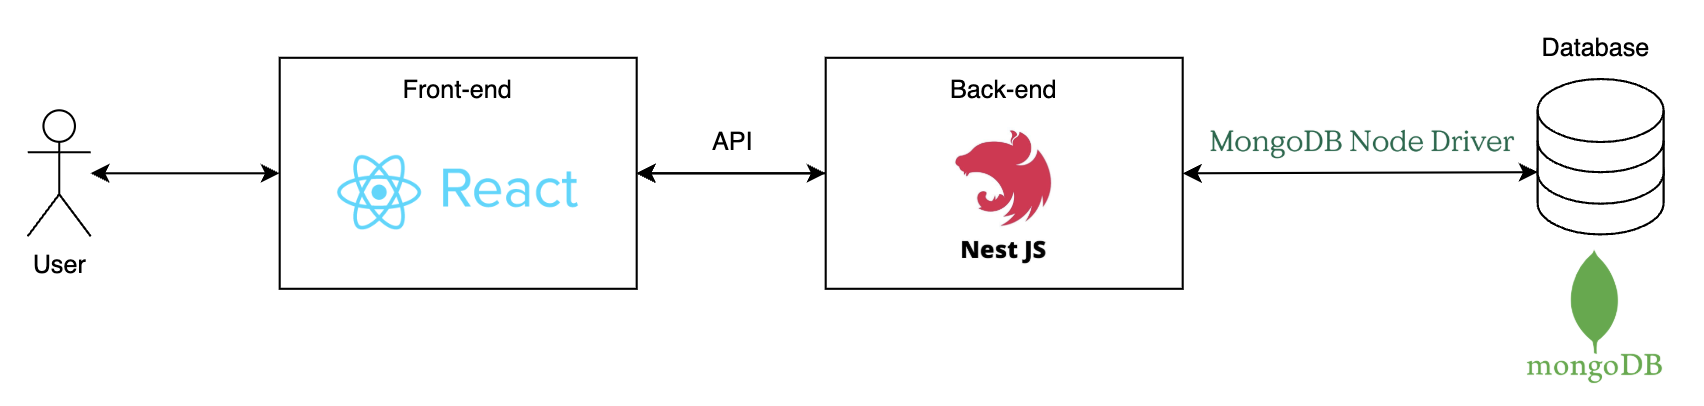
\includegraphics[width=\linewidth]{DBMS-Application/Images/dbms-architecture.png}
    \caption{Kiến trúc hệ thống}
\end{figure}

Kiến trúc của hệ thống là \textbf{Client-Server Architecture}, cụ thể là \textbf{3-Tier Architecture} (kiến trúc 3 lớp), gồm các tầng sau:
\begin{itemize}
    \item \textbf{Tầng Presentation (Client)}:
    \begin{itemize}
        \item Thành phần: \textbf{React.JS (Front-end)}
        \item Vai trò: Hiển thị giao diện người dùng, xử lý các thao tác và yêu cầu từ phía người dùng. Tầng này gọi API từ Back-end và hiển thị dữ liệu trả về.
    \end{itemize}

    \item \textbf{Tầng Application Logic (Server)}:
    \begin{itemize}
        \item Thành phần: \textbf{Nest.JS (Back-end)}
        \item Vai trò: Xử lý logic nghiệp vụ, xác thực người dùng, điều hướng các yêu cầu đến cơ sở dữ liệu, và trả kết quả về cho Front-end thông qua API.
        \item Kết nối tới cơ sở dữ liệu sử dụng \textbf{MongoDB Node Driver}.
    \end{itemize}

    \item \textbf{Tầng Data (Database)}:
    \begin{itemize}
        \item Thành phần: \textbf{MongoDB}
        \item Vai trò: Lưu trữ và quản lý dữ liệu của hệ thống, xử lý các thao tác truy vấn, thêm, sửa, xóa dữ liệu.
    \end{itemize}
\end{itemize}

\textbf{Quy trình hoạt động}:

\begin{figure}[H]
    \centering
    \begin{tikzpicture}[node distance=1.5cm]
    % Các khối trong quy trình
    \node (user) [startstop] {1. Người dùng tương tác với giao diện (Xem danh sách công việc, ứng tuyển công việc,...)};
    \node (frontend) [process, below of=user] {2. Front-end gửi request đến Back-end qua API};
    \node (api) [process, below of=frontend] {3. Back-end xử lý logic nghiệp vụ và truy vấn CSDL MongoDB};
    \node (response) [process, below of=api] {4. Back-end gửi phản hồi về Front-end};
    \node (display) [startstop, below of=response] {5. Front-end hiển thị dữ liệu lên giao diện người dùng};
    
    % Vẽ các mũi tên
    \draw [arrow] (user) -- (frontend);
    \draw [arrow] (frontend) -- (api);
    \draw [arrow] (api) -- (response);
    \draw [arrow] (response) -- (display);
    
    \end{tikzpicture}
\end{figure}
\subsection{Hiện thực hệ thống}

\textbf{Link github dự án}: \href{https://github.com/dasabu/matchjob-dbms-asgmt-version}{https://github.com/dasabu/matchjob-dbms-asgmt-version}\\

\textbf{Chạy dự án (môi trường local)}:
\begin{enumerate}
    \item Clone dự án: \texttt{git clone https://github.com/dasabu/matchjob-dbms-asgmt-version}
    \item Chạy back-end:
    \begin{itemize}
        \item Chuyển đến thư mục \texttt{backend}: \texttt{cd backend}
        \item Cài đặt các dependencies cần thiết: \texttt{npm install}
        \item Start server: \texttt{npm run start:dev}
    \end{itemize}
    \item Chạy front-end:
    \begin{itemize}
        \item Chuyển đến thư mục \texttt{frontend}: \texttt{cd frontend}
        \item Cài đặt các dependencies cần thiết: \texttt{npm install}
        \item Start client:
        \texttt{npm run dev}
    \end{itemize}

    \item Truy cập vào ứng dụng:
    \begin{itemize}
        \item Backend: \texttt{http://localhost:3333}
        \item Frontend: \texttt{http://localhost:3004}
    \end{itemize}
\end{enumerate}

\textbf{Lưu ý}: Cần phải cài đặt \href{https://nodejs.org/en}{\textbf{Node.js Runtime}} và \href{https://www.mongodb.com/docs/manual/installation/}{\textbf{MongoDB}} để chạy được dự án

% \subsubsection{Kết nối Backend - Database}

Trong hệ thống backend, nhóm tạo một module riêng biệt được dùng cho việc quản lý kết nối và truy cập đến cơ sở dữ liệu là \textbf{MongoModule}. Trong module này, \textbf{MongoService} là service được nhóm định nghĩa nhằm khởi tạo kết nối với database của hệ thống khi module khởi chạy và cung cấp đối tượng \texttt{Db} (đại diện cho cơ sở dữ liệu của hệ thống), thông qua một phương thức chung \texttt{getDatabase} cho các service khác sử dụng.

\begin{lstlisting}
import { Injectable, OnModuleDestroy, OnModuleInit } from '@nestjs/common';
import { MongoClient, Db } from 'mongodb';

@Injectable()
export class MongoService implements OnModuleInit, OnModuleDestroy {
    private client: MongoClient;    // Object MongoClient de quan ly ket noi
    private db: Db;                 // Object Db de truy cap vao database

    // Khoi tao ket noi khi module duoc khoi chay
    async onModuleInit() {
        const uri = process.env.MONGO_URI;
        const dbName = process.env.MONGO_DB_NAME;
        
        this.client = new MongoClient(uri);
        await this.client.connect();
        this.db = this.client.db(dbName);
        console.log(`Connected to MongoDB: ${dbName}`);
    }

    // Cung cap database cho cac module khac
    getDatabase(): Db {
        if (!this.db) {
          throw new Error('Database connection is not initialized');
        }
        return this.db;
    }

    // Dong ket noi khi module bi huy
    async onModuleDestroy() {
        await this.client.close();
        console.log('Disconnected from MongoDB');
    }
}
\end{lstlisting}

Khi đó, các module khác sẽ sử dụng \textbf{MongoService} đã khai báo ở trên để truy cập trực tiếp vào cơ sở dữ liệu của hệ thống để thực hiện các truy vấn cần thiết. Ví dụ, \textbf{JobsService} (nơi xử lý logic nghiệp vụ liên quan đến các thực thể công việc của hệ thống) sẽ \textbf{import} \textbf{MongoService} vào và thực hiện truy vấn "Danh sách các công việc đang tuyển dụng":

\begin{lstlisting}
import { Injectable, OnModuleInit } from '@nestjs/common';
import { Db } from 'mongodb';
import { MongoService } from './mongo.service';

@Injectable()
export class JobsService implements OnModuleInit {
    private db: Db;
    constructor(private mongoService: MongoService) {}
    
    // Khoi tao database tu MongoService khi module khoi chay
    onModuleInit() {
        this.db = this.mongoService.getDatabase();
    }
    
    // Vi du: Tra ve tat ca cac cong viec dang tuyen dung
    async getAllJobs() {
        return this.db      // Truy cap vao CSDL cua he thong
        .collection('jobs') // Truy cap vao collection 'jobs'
        .find({})           // Tim tat ca cac cong viec
        .toArray();         // Chuyen ket qua ve dang mang
    }
}
\end{lstlisting}

% \subsubsection{Giao diện người dùng - Trang chủ}

Trang chủ của website cung cấp thông tin trực quan, đầy đủ về các công việc mới nhất như sau:

\begin{figure}[H]
    \centering
    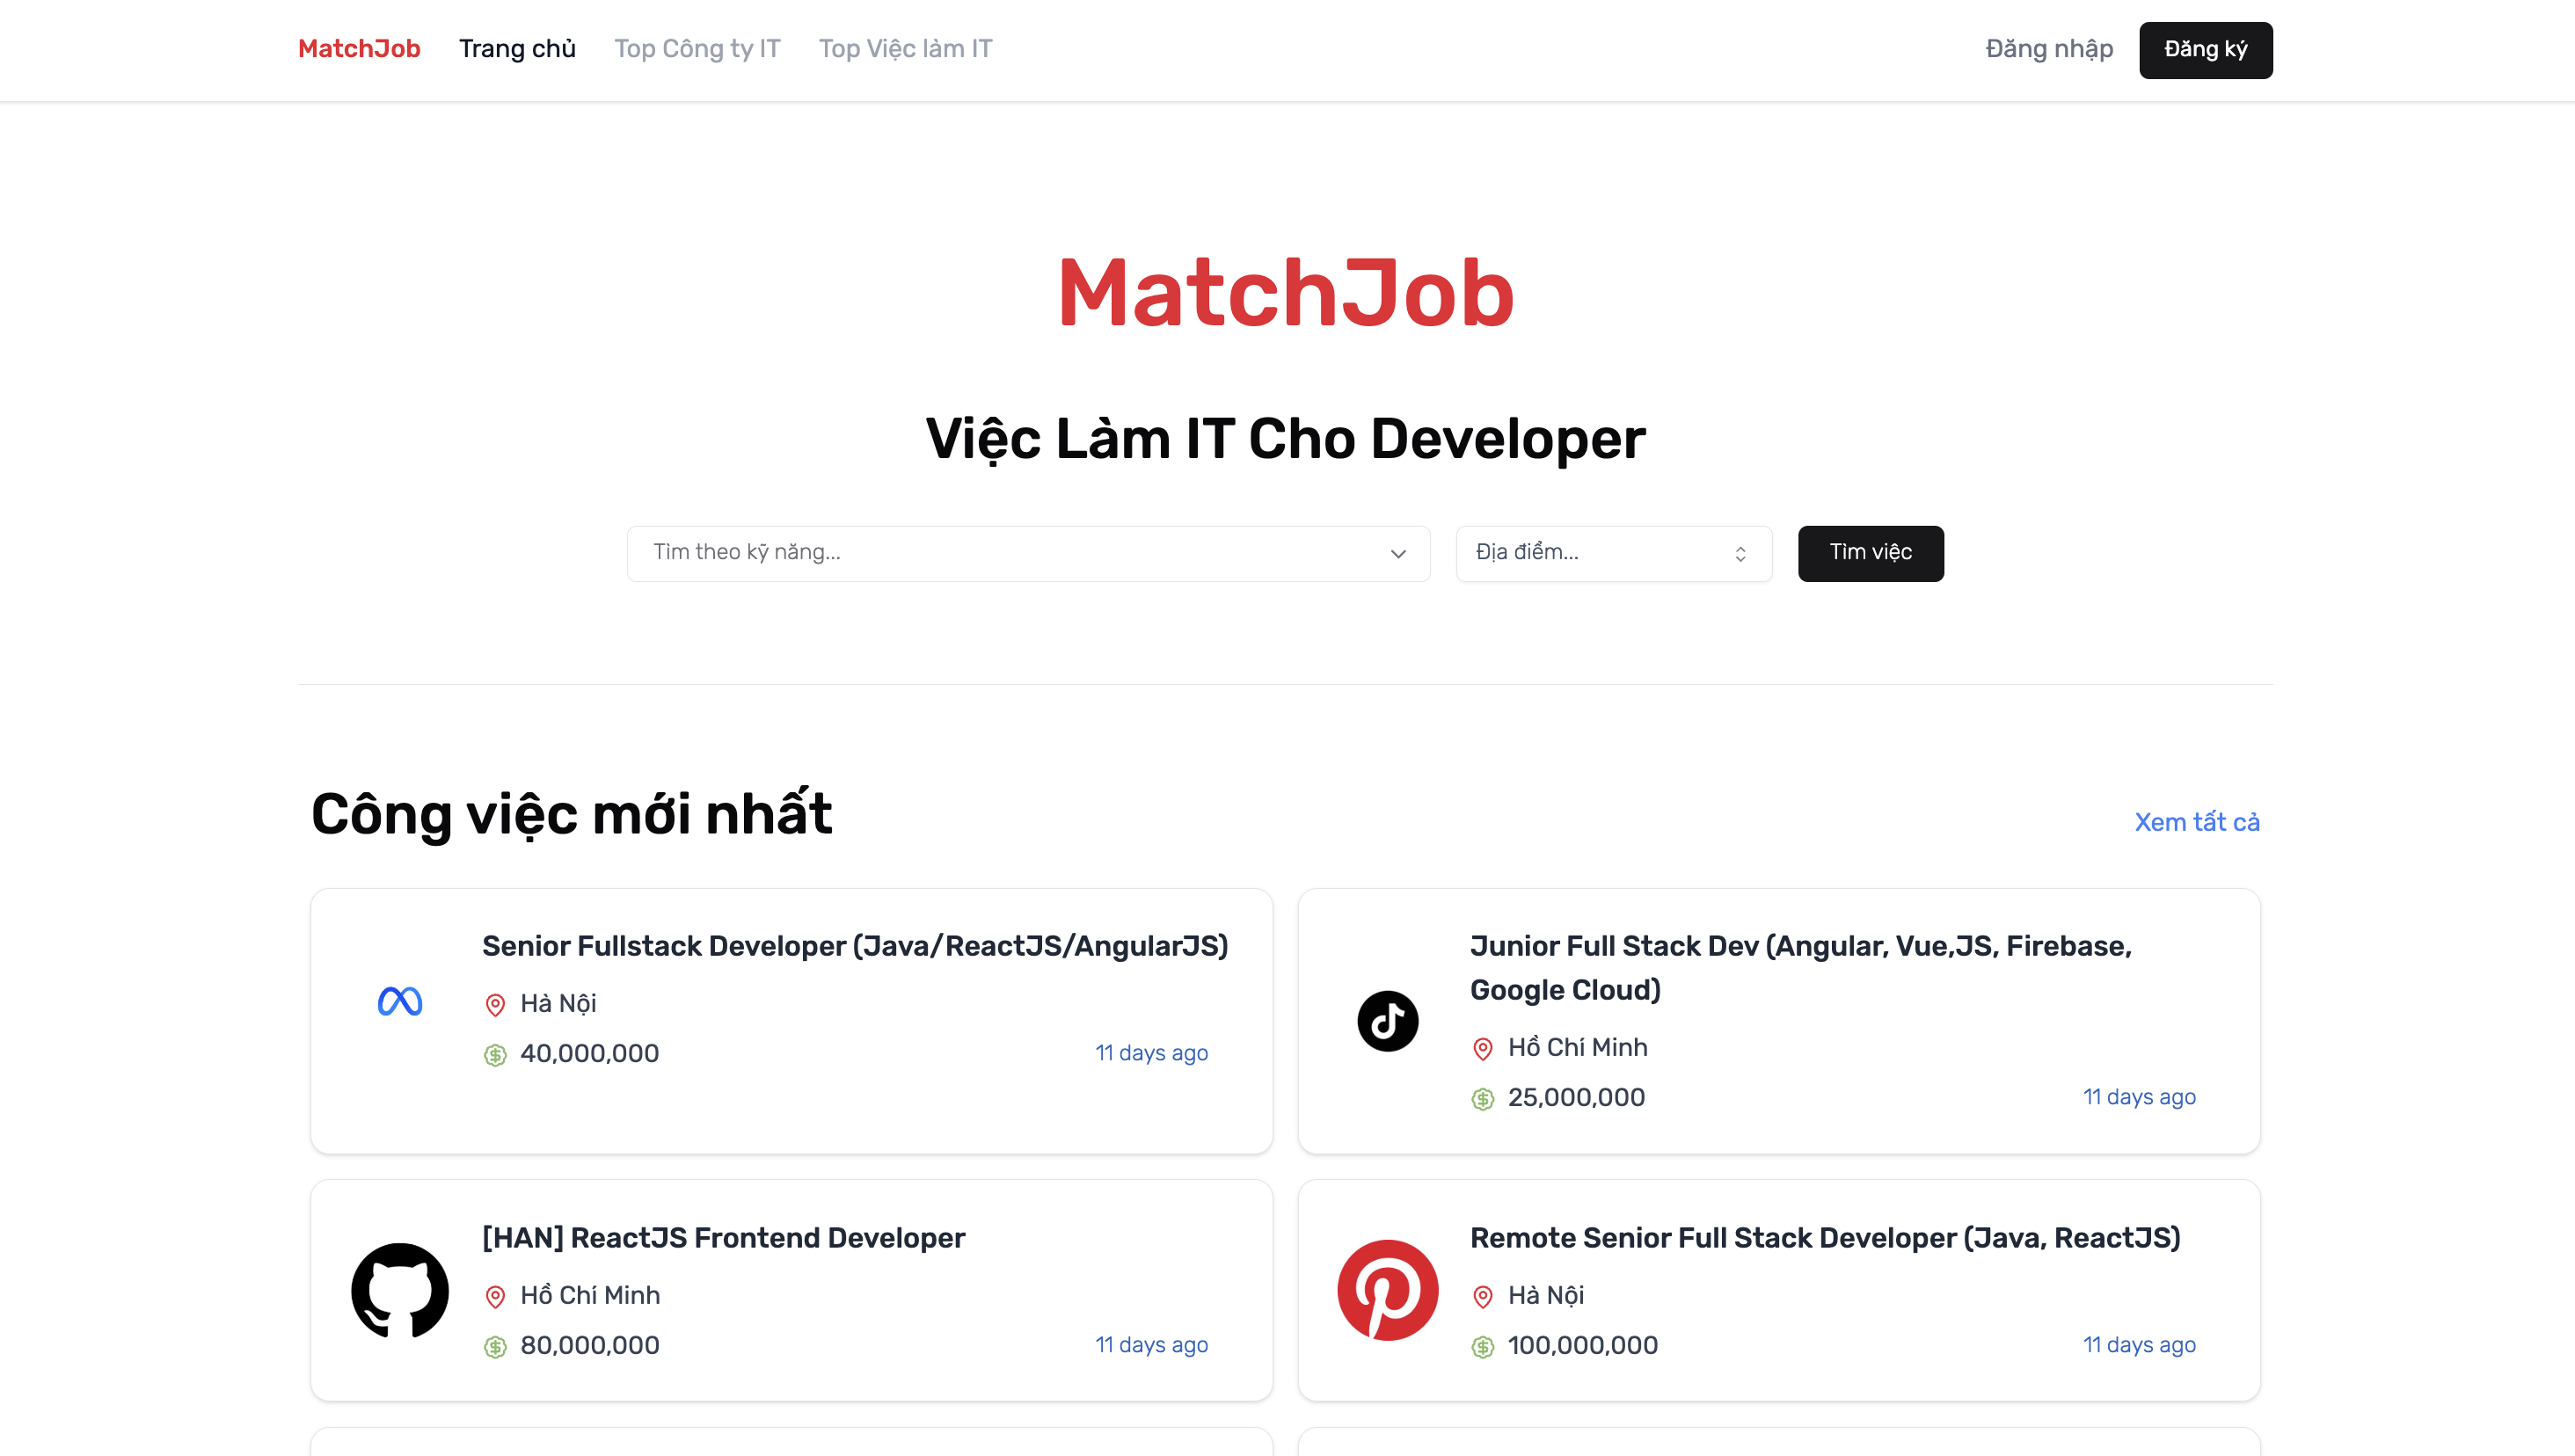
\includegraphics[width=\linewidth]{DBMS-Application/Images/user-screen-job.png}
    \caption{Trang chủ - Danh sách công việc đang tuyển dụng}
    \label{fig:homepage-job}
\end{figure}

Truy vấn sử dụng: \textbf{Query with composite condition}
\begin{lstlisting}
async findAll(current: number, pageSize: number, qs: string) {
    // Loc ra dieu kien filter va sort tu query parameters
    const { filter } = aqp(qs);

    // Truy van: Danh sach cong viec thoa man dieu kien filter
    const jobs = await this.db
      .collection('jobs')
      .find(filter)
      .skip((current - 1) * pageSize)
      .limit(pageSize)
      .toArray();

    // Tra ve response cho Frontend
    return jobs;
}
\end{lstlisting}

Giải thích:

\begin{enumerate}
    \item Frontend sẽ tự động gửi yêu cầu đến Backend thông qua API:
    \begin{lstlisting}[numbers=none]
GET /api/jobs?current=0&pageSize=6
    \end{lstlisting}
    
    \item Backend sẽ nhận được query parameters (\texttt{current} và \texttt{pageSize}) từ Frontend và thực hiện truy vấn CSDL với filter và phân trang:
    \begin{itemize}
        \item Sử dụng \texttt{find()} để lọc dữ liệu theo điều kiện \texttt{filter} (trong trường hợp này, \texttt{filter} là object rỗng (\texttt{\{\}}) nên sẽ trả về tất cả các công việc có trong hệ thống)
        \item Sử dụng \texttt{skip()} để bỏ qua các bản ghi không cần thiết
        \item Sử dụng \texttt{limit()} để giới hạn số lượng bản ghi trả về
    \end{itemize}

    \item Sau khi truy vấn được thực hiện thành công, Backend phản hồi danh sách các công việc cho Frontend để hiển thị lên giao diện người dùng
\end{enumerate}

Người dùng có thể tìm kiếm công việc bằng cách lọc theo \textbf{Địa điểm} và \textbf{Kỹ năng yêu cầu}. Ví dụ, tìm các công việc có yêu cầu kỹ năng \textbf{"React.JS"} và \textbf{"React Native"} tại \textbf{TP. Hồ Chí Minh}, hệ thống sẽ hiện lên một pop-up chứa các công việc thoả mãn.

\begin{figure}[H]
    \centering
    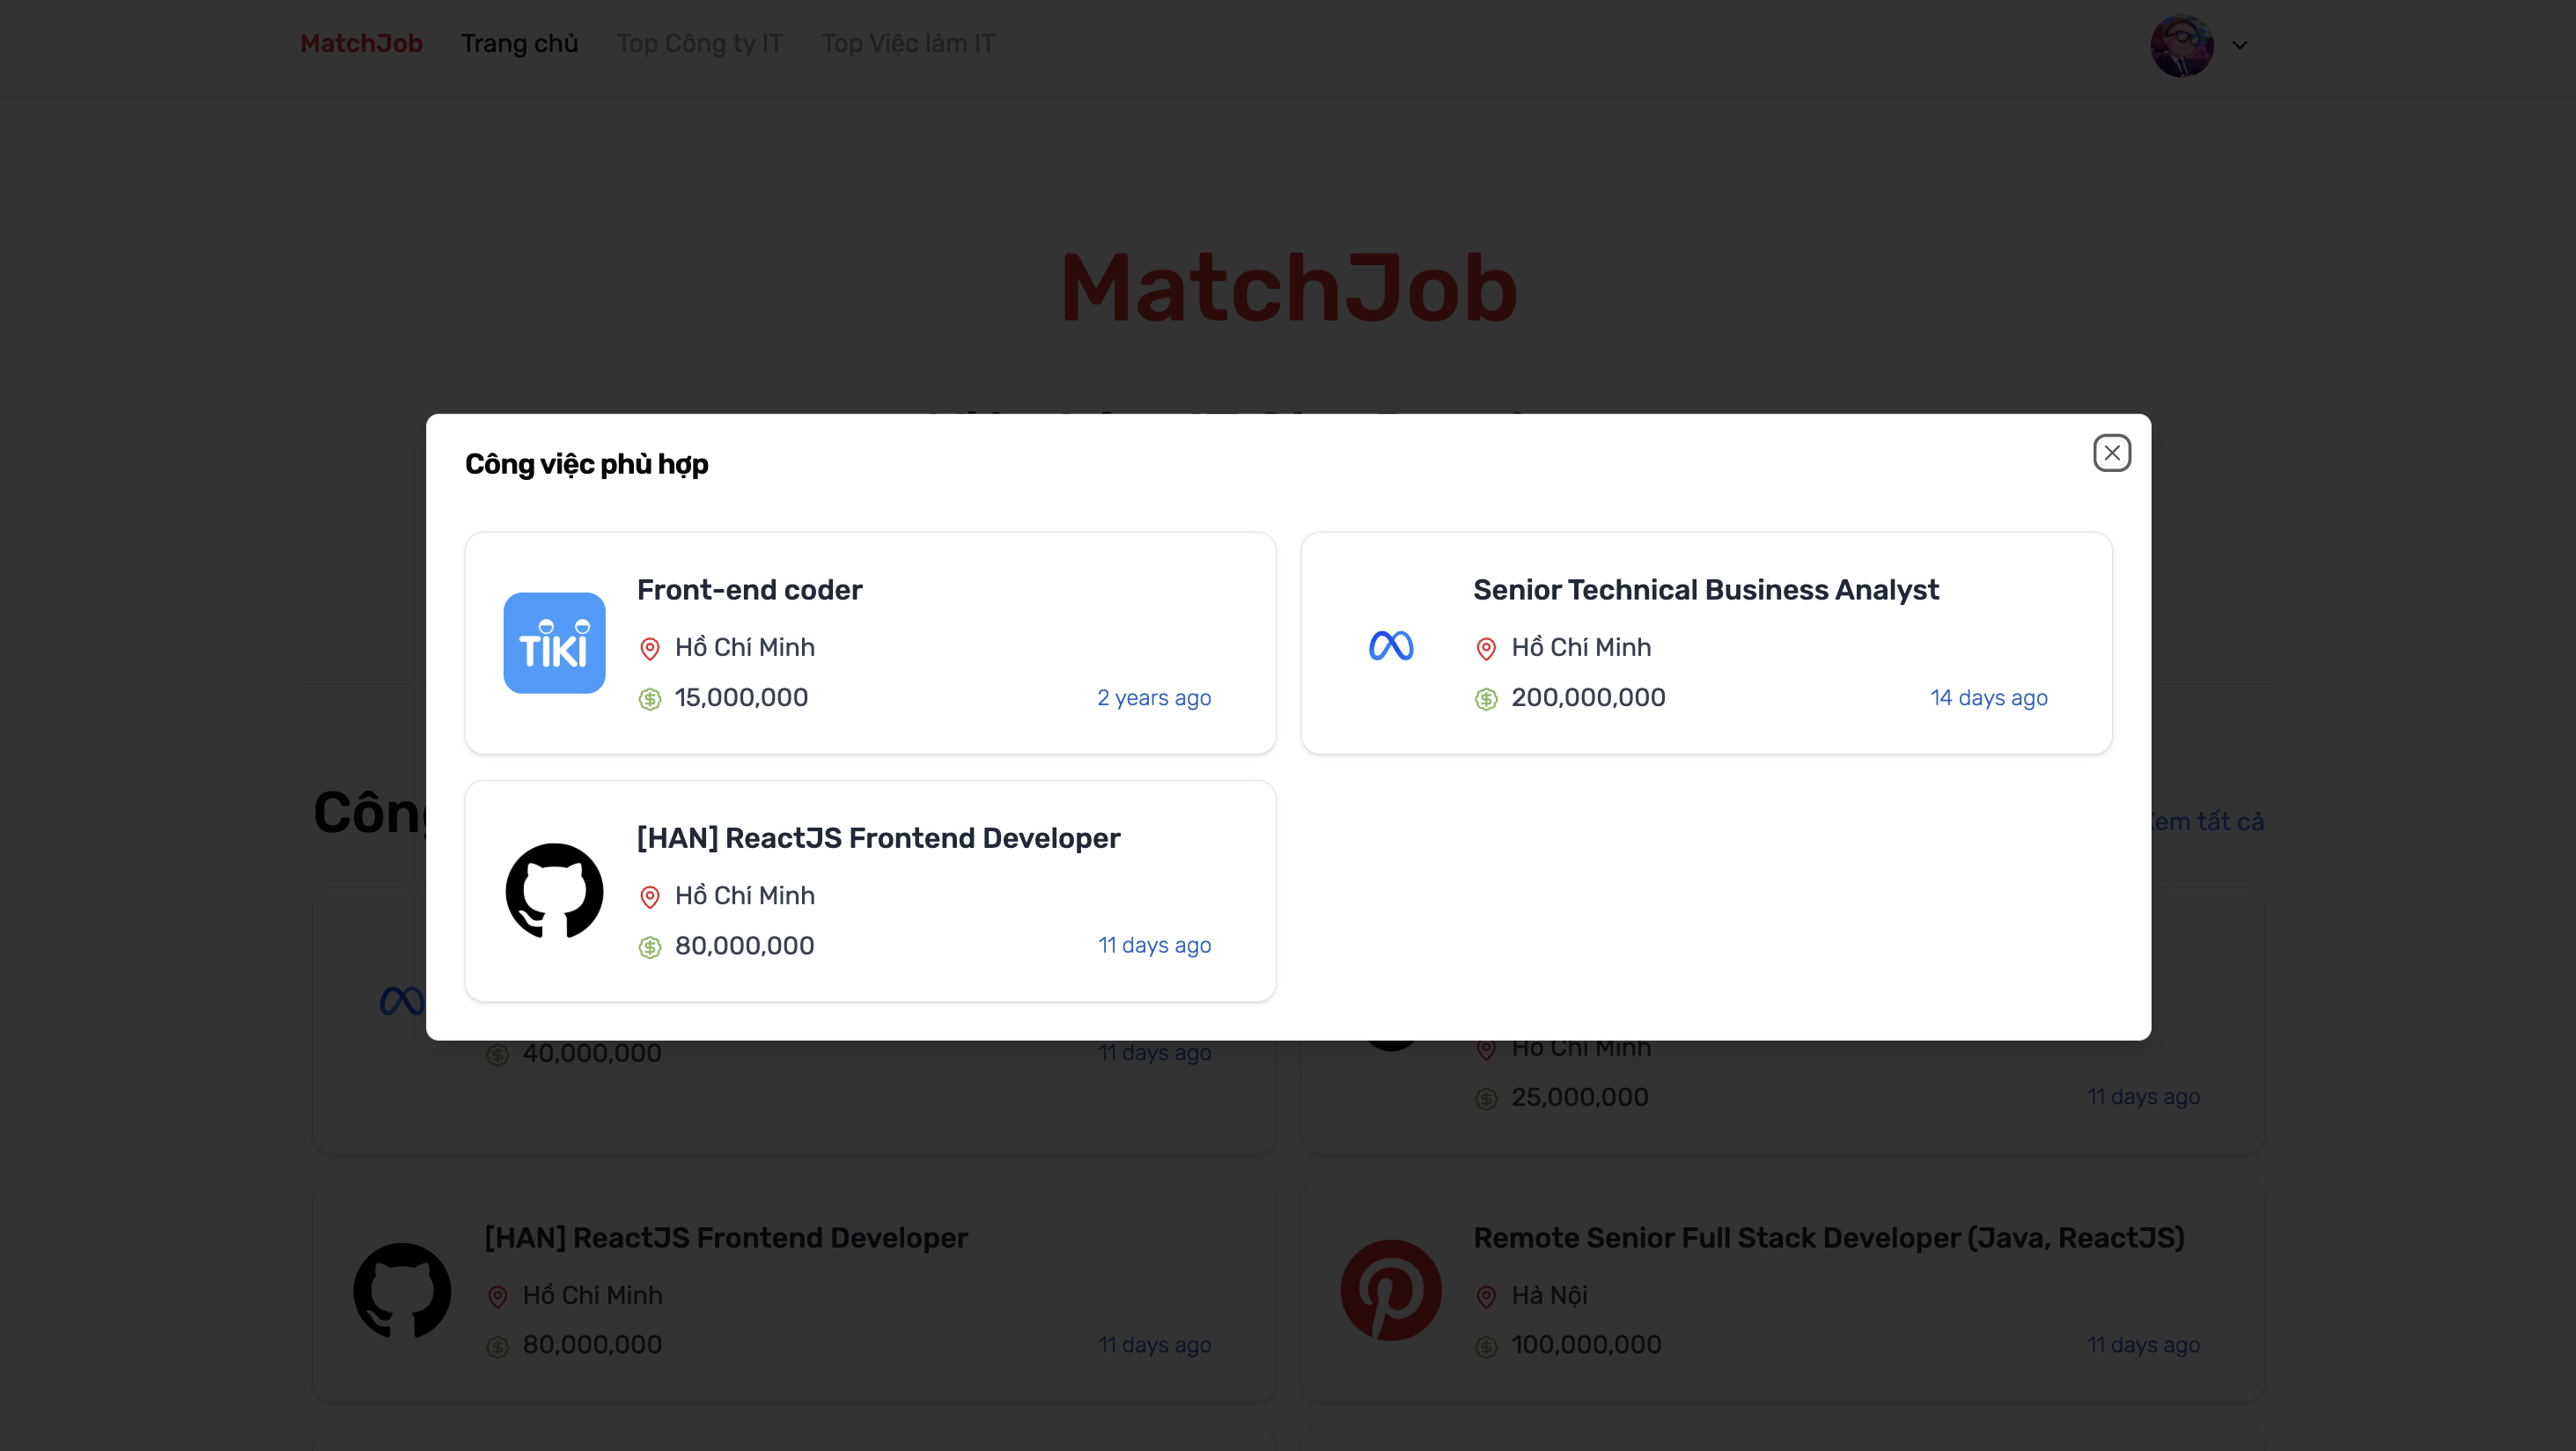
\includegraphics[width=\linewidth]{DBMS-Application/Images/modal-job-search.png}
    \caption{Trang chủ - Lọc công việc theo Địa điểm và Kỹ năng}
    \label{fig:homepage-job-search-filter}
\end{figure}

Truy vấn sử dụng: \textbf{Query with single/composite condition}

\begin{lstlisting}
async getJobsByLocationAndSkills(location: string, skills: string[]) {
    const query: { location?: string; skills?: { $in: string[] } } = {};

    if (location) query.location = location; 
    if (skills.length > 0) query.skills = { $in: skills }; 
    // query = { location: 'HOCHIMINH', skills: { $in: ['REACT.JS', 'REACT NATIVE'] } }

    // Truy van: Loc cac cong viec theo Ky nang va Dia diem
    return await this.db // Truy cap vao database he thong
    .collection('jobs')  // Truy cap vao collection 'jobs'
    .find(query)         // Loc theo dieu kien 'location' va 'skills' trong query
    .toArray();          // Chuyen ket qua ve dang mang
  }
\end{lstlisting}

Giải thích truy vấn:
\begin{itemize}
    \item Back-end nhận được yêu cầu từ Front-end, chứa 2 tham số \texttt{location} và \texttt{skills} trong query parameters và thực hiện xây dựng điều kiện lọc \texttt{query} với các giá trị đó
    
    Ví dụ: \texttt{ query = \{ location : ’HOCHIMINH’, skills : \{ \$in : [ ’REACT.JS’, ’REACT NATIVE’] \} \} }

    \item Sau đó, Back-end sẽ thực hiện truy vấn đến CSDL để lọc ra các công việc thoả mãn điều kiện vừa xây dựng được, và phản hồi về cho Front-end khi thành công
\end{itemize}

Người dùng cũng có thể xem được các công ty tuyển dụng hàng đầu cùng một số thông tin như: tên, logo công ty, số lượng công việc đang tuyển và thu thập cao nhất.

\begin{figure}[H]
    \centering
    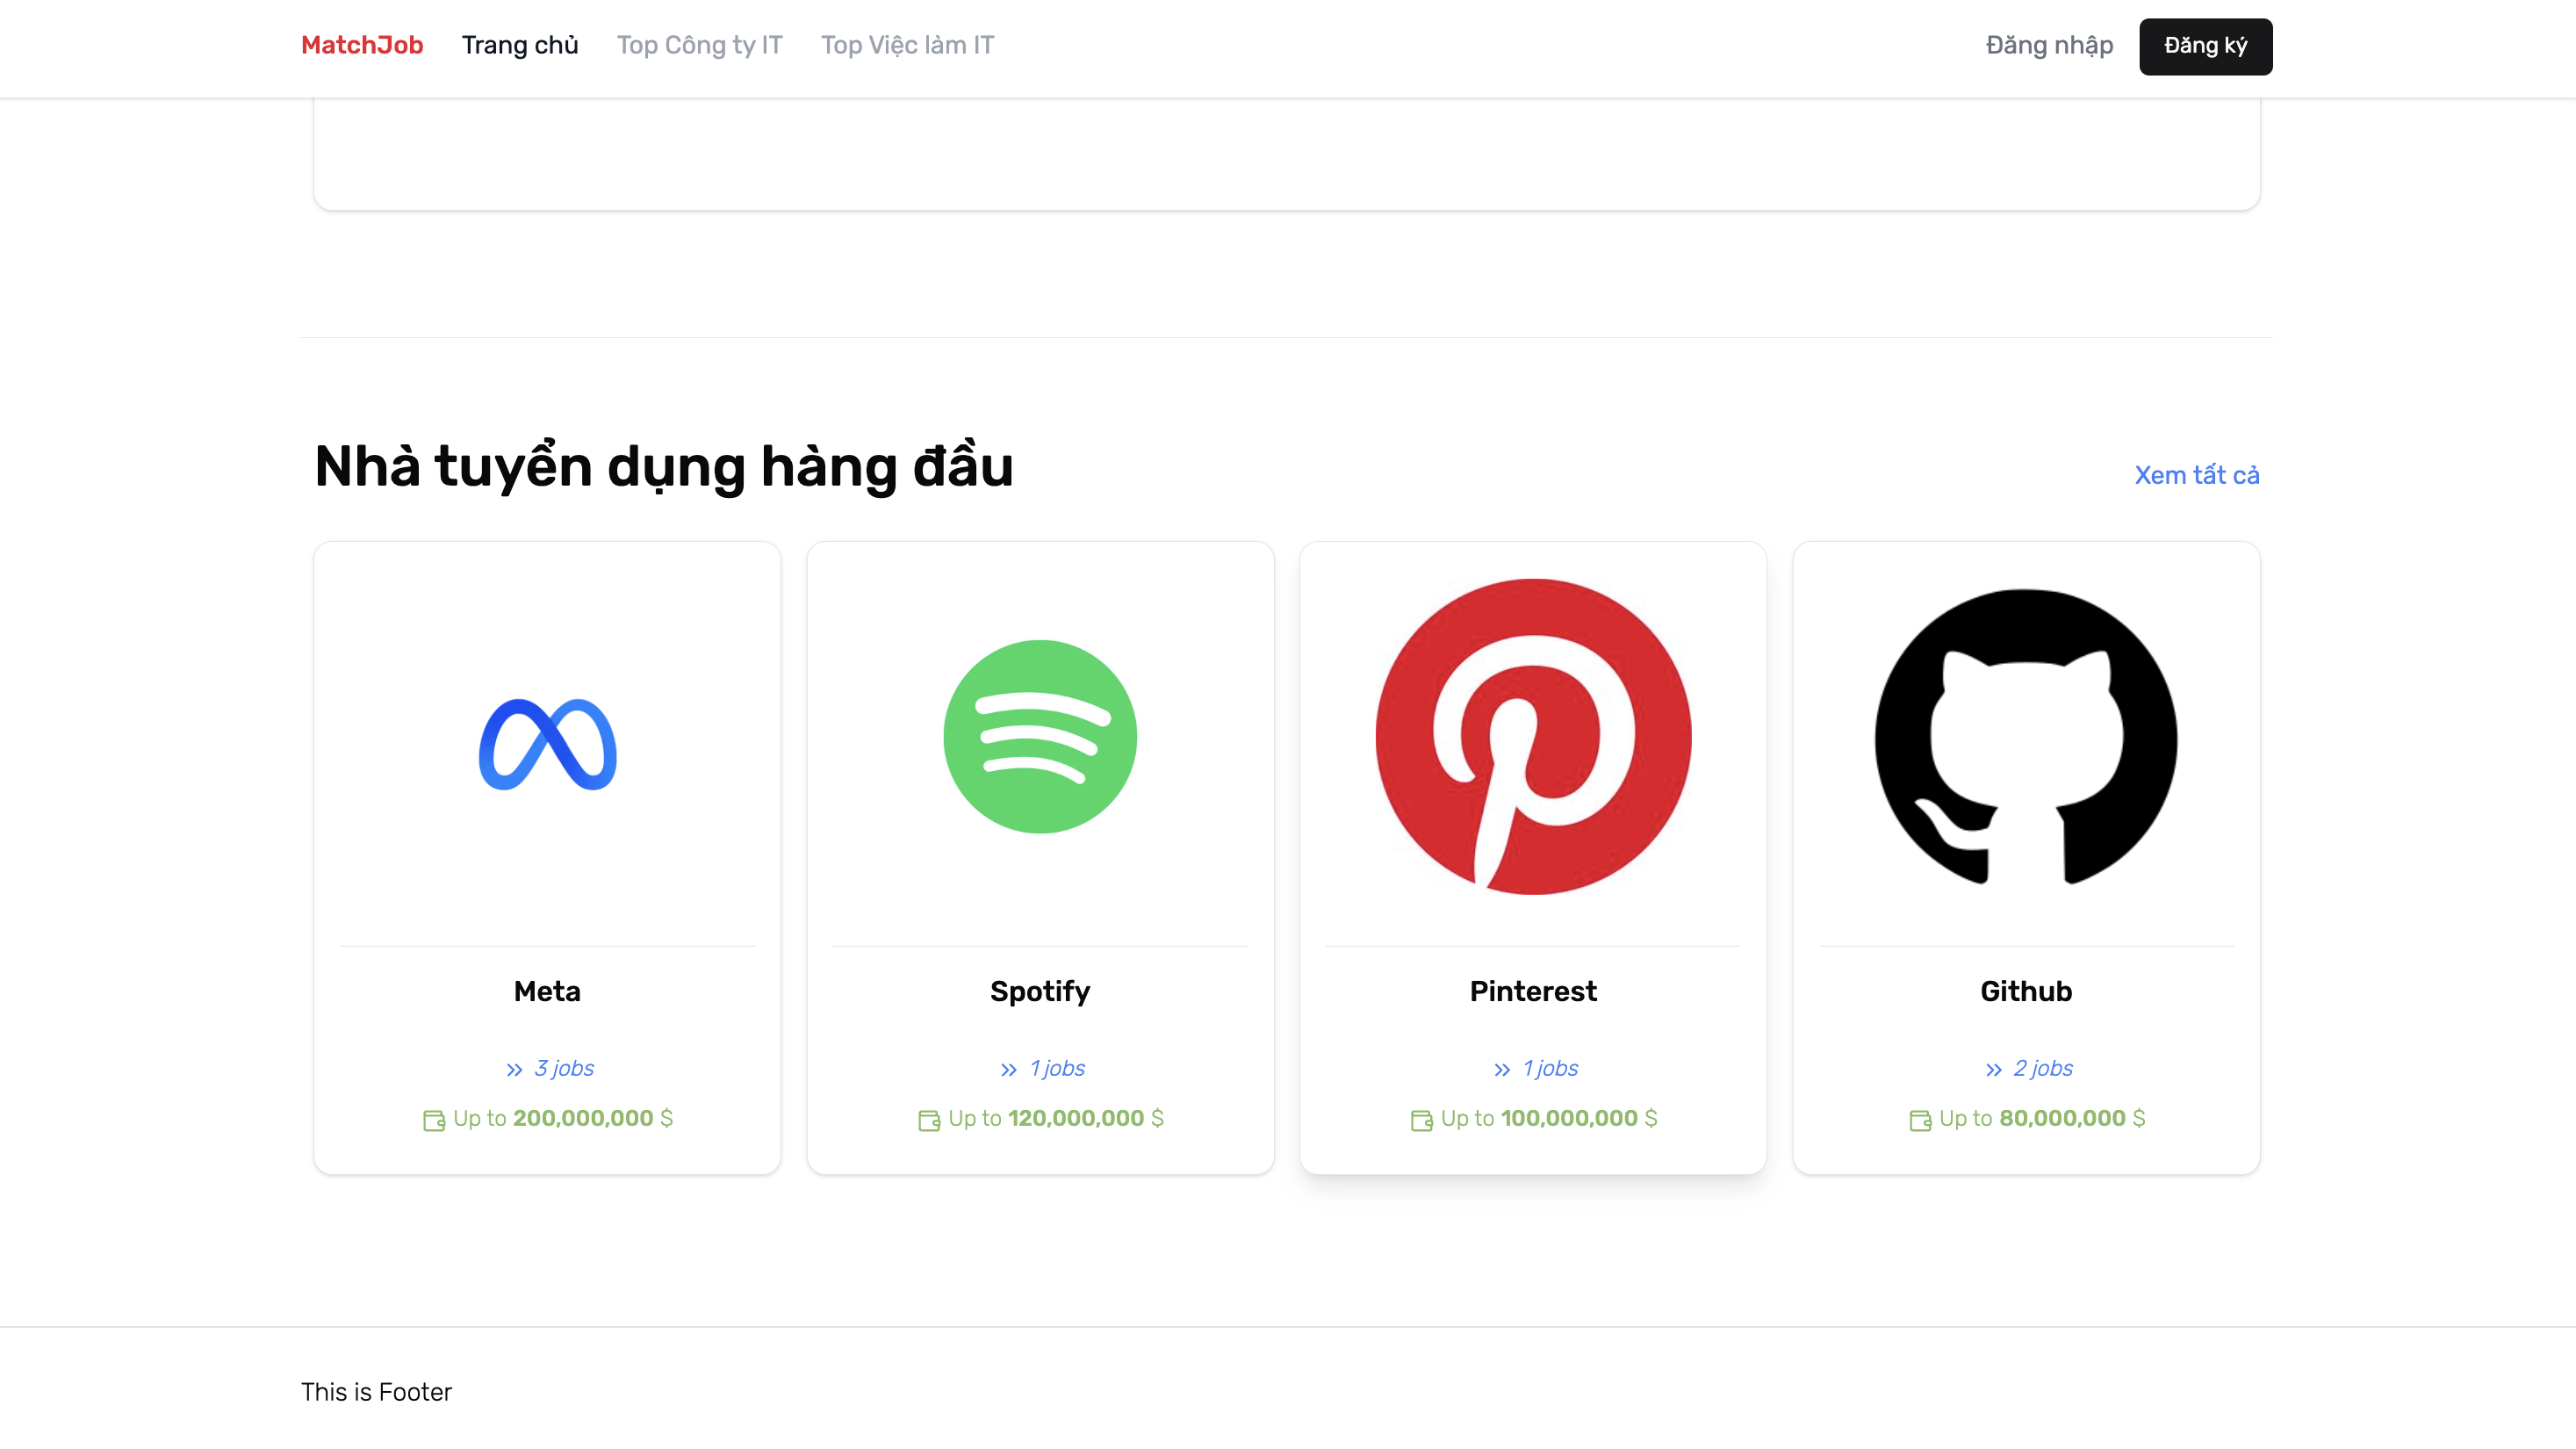
\includegraphics[width=\linewidth]{DBMS-Application/Images/user-screen-company.png}
    \caption{Trang chủ - Danh sách công ty tuyển dụng hàng đầu}
    \label{fig:homepage-company}
\end{figure}

Truy vấn sử dụng:
\begin{itemize}
    \item \textbf{Query with join}: Sử dụng và \texttt{\$lookup} để join collections \textbf{companies} với \textbf{jobs}
    \item \textbf{Query with aggregation functions}: Sử dụng \texttt{\$size}, \texttt{\$max}, \texttt{\$reduce} để tính toán số lượng công việc, mức lương cao nhất của công ty
\end{itemize}

\begin{lstlisting}
const pipeline = [
  { $match: filter },
  {
    $lookup: {
      from: 'jobs',
      let: { companyId: { $toString: '$_id' } },
      pipeline: [
        {
          $match: {
            $expr: {
              $eq: ['$company._id', '$$companyId'],
            },
          },
        },
      ],
      as: 'jobs',
    },
  },
  {
    $project: {
      _id: 1,
      name: 1,
      address: 1,
      description: 1,
      logo: 1,
      totalJobs: { $size: '$jobs' }, // Dem so luong cong viec
      maxSalary: { $max: '$jobs.salary' }, // Lay ra salary cao nhat
      maxSalaryJobId: {
        $reduce: {
          input: '$jobs',
          initialValue: null,
          in: {
            $cond: [
              { $eq: ['$$this.salary', { $max: '$jobs.salary' }] },
              '$$this._id',
              '$$value',
            ],
          },
        },
      },
    },
  },
  { $sort: { maxSalary: -1 } }, // Sap xep cong ty giam dan theo maxSalary
  { $skip: offset },
  { $limit: limit },
];

return await this.db
  .collection('companies')
  .aggregate(pipeline)
  .toArray();
\end{lstlisting}

Giải thích truy vấn: 
\begin{itemize}
    \item \texttt{\$match}: Lọc các công ty thỏa mãn điều kiện.
    \item \texttt{\$lookup}: Join collection \textbf{companies} (\texttt{\_id}) collection \textbf{jobs} (\texttt{companyId}) để lấy các công việc ứng với từng công ty
    \item \texttt{\$project}: Lọc ra các trường trong collection \textbf{companies} như \texttt{\_id}, \texttt{name}, \texttt{address}, \texttt{logo} và Tính toán các thông tin thống kê như số lượng công việc (\texttt{totalJobs}), lương cao nhất (\texttt{maxSalary}) và ID công việc có lương cao nhất (\texttt{maxSalaryJobId}) của từng công ty
    \item \texttt{\$sort}: Sắp xếp các công ty giảm dần theo lương cao nhất (\texttt{maxSalary})
    \item \texttt{\$skip} và \texttt{\$limit}: Phân trang kết quả
\end{itemize}

Bên cạnh đó, người dùng có thể xem nhanh thông tin các công việc đang tuyển dụng của một công ty cụ thể, thông qua các thẻ công ty được hiển thị:

\begin{figure}[H]
    \centering
    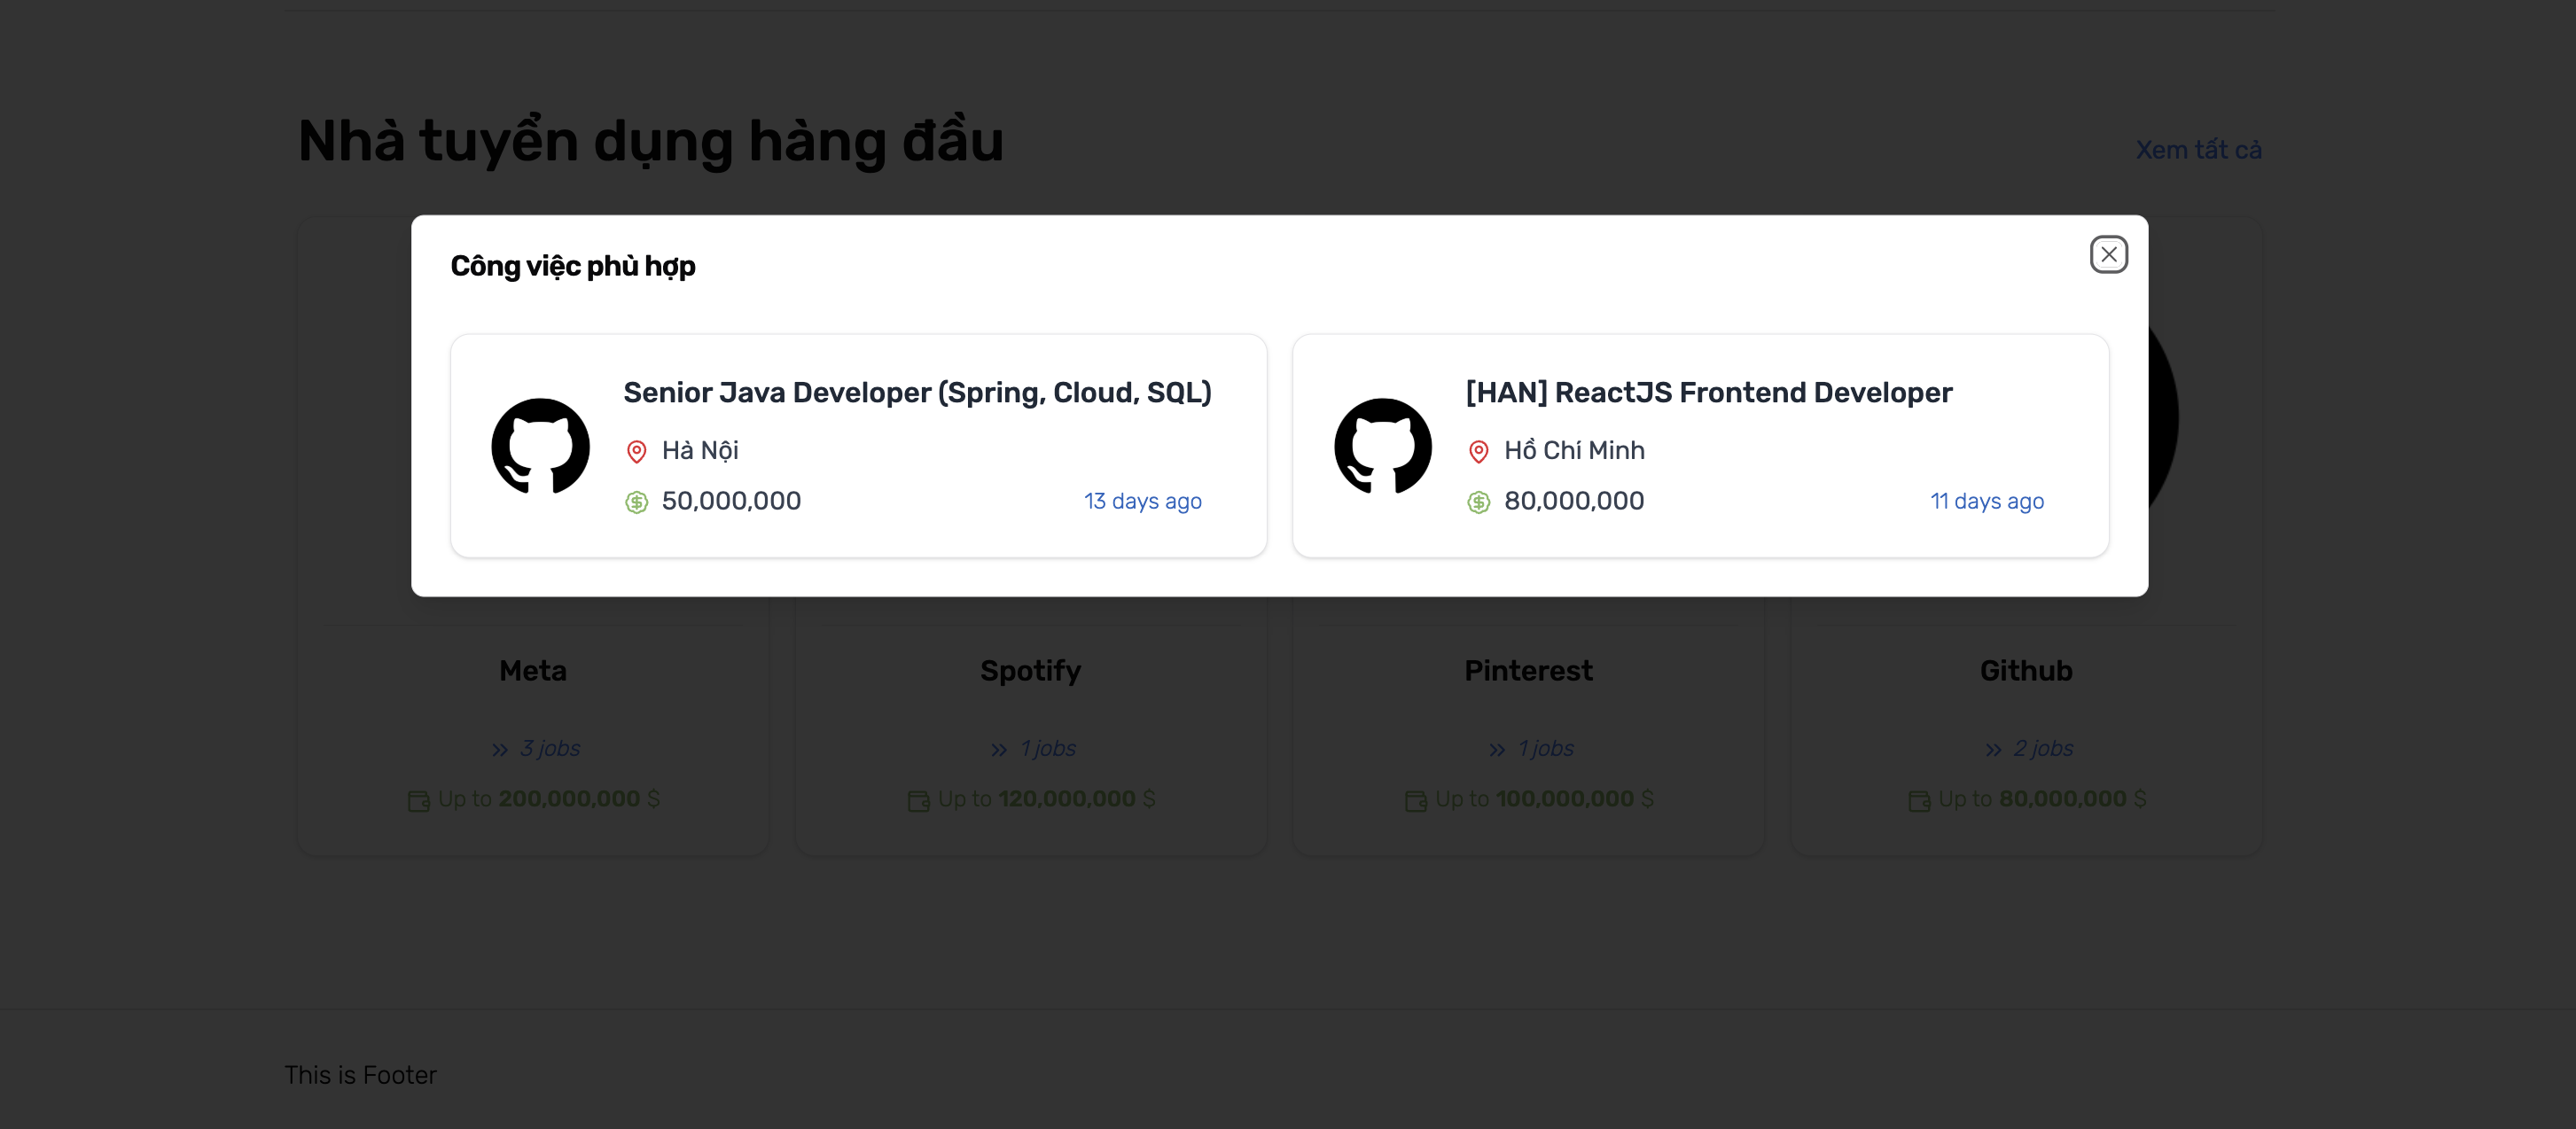
\includegraphics[width=\linewidth]{DBMS-Application/Images/modal-job-company.png}
    \caption{Trang chủ - Lọc ra các công việc thuộc một công ty cụ thể}
    \label{fig:homepage-job-company}
\end{figure}

Truy vấn sử dụng:
\begin{itemize}
    \item \textbf{Query with single condition}: Lọc document cụ thể từ collection \textbf{companies} dựa trên \texttt{\_id}

    \item \textbf{Query with join}: Thực hiện join giữa collection \textbf{companies} và \textbf{jobs} để lấy công việc liên quan
\end{itemize}

\begin{lstlisting}
const pipeline = [
  {
    $match: { _id: new ObjectId(companyId) }, // Loc ra cong ty co _id = companyId duoc truyen vao
  },
  {
    $lookup: {
      from: 'jobs', // Join collection 'companies' voi collection 'jobs'
      let: { companyId: { $toString: '$_id' } },
      pipeline: [
        {
          $match: {
            $expr: { $eq: ['$company._id', '$$companyId'] },
          },
        },
      ],
      as: 'jobs', // Luu ket qua vao field 'jobs' cho tung cong ty
    },
  },
  {
    $project: { // Loc ra cac field can thiet
      _id: 1,
      name: 1,
      address: 1,
      description: 1,
      logo: 1,
      jobs: 1,
    },
  },
];

return await this.db
  .collection('companies')
  .aggregate(pipeline)
  .toArray();
\end{lstlisting}

Giải thích truy vấn:
\begin{itemize}
    \item \texttt{\$match}: Lọc công ty cụ thể từ collection companies dựa trên \texttt{\_id} được truyền vào (\texttt{companyId}).
    
    \item \texttt{\$lookup}: Join collection \textbf{companies} với collection \textbf{jobs} để tìm tất cả các công việc thuộc công ty đó, bằng cách so sánh \texttt{\_id} của công ty trong \textbf{companies} với \texttt{company.\_id} trong \textbf{jobs} và lưu danh sách công việc vào trường \textbf{jobs}.


    \item \texttt{\$project}: Chọn các trường cần trả về gồm \texttt{\_id}, \texttt{name}, \texttt{address}, \texttt{description}, \texttt{logo}, và \texttt{jobs}.
\end{itemize}

Cuối cùng, người dùng có thể xem thống kê các kỹ năng có nhu cầu tuyển dụng nhiều, được thu thập từ các công việc đang được tuyển dụng:

\begin{figure}[H]
    \centering
    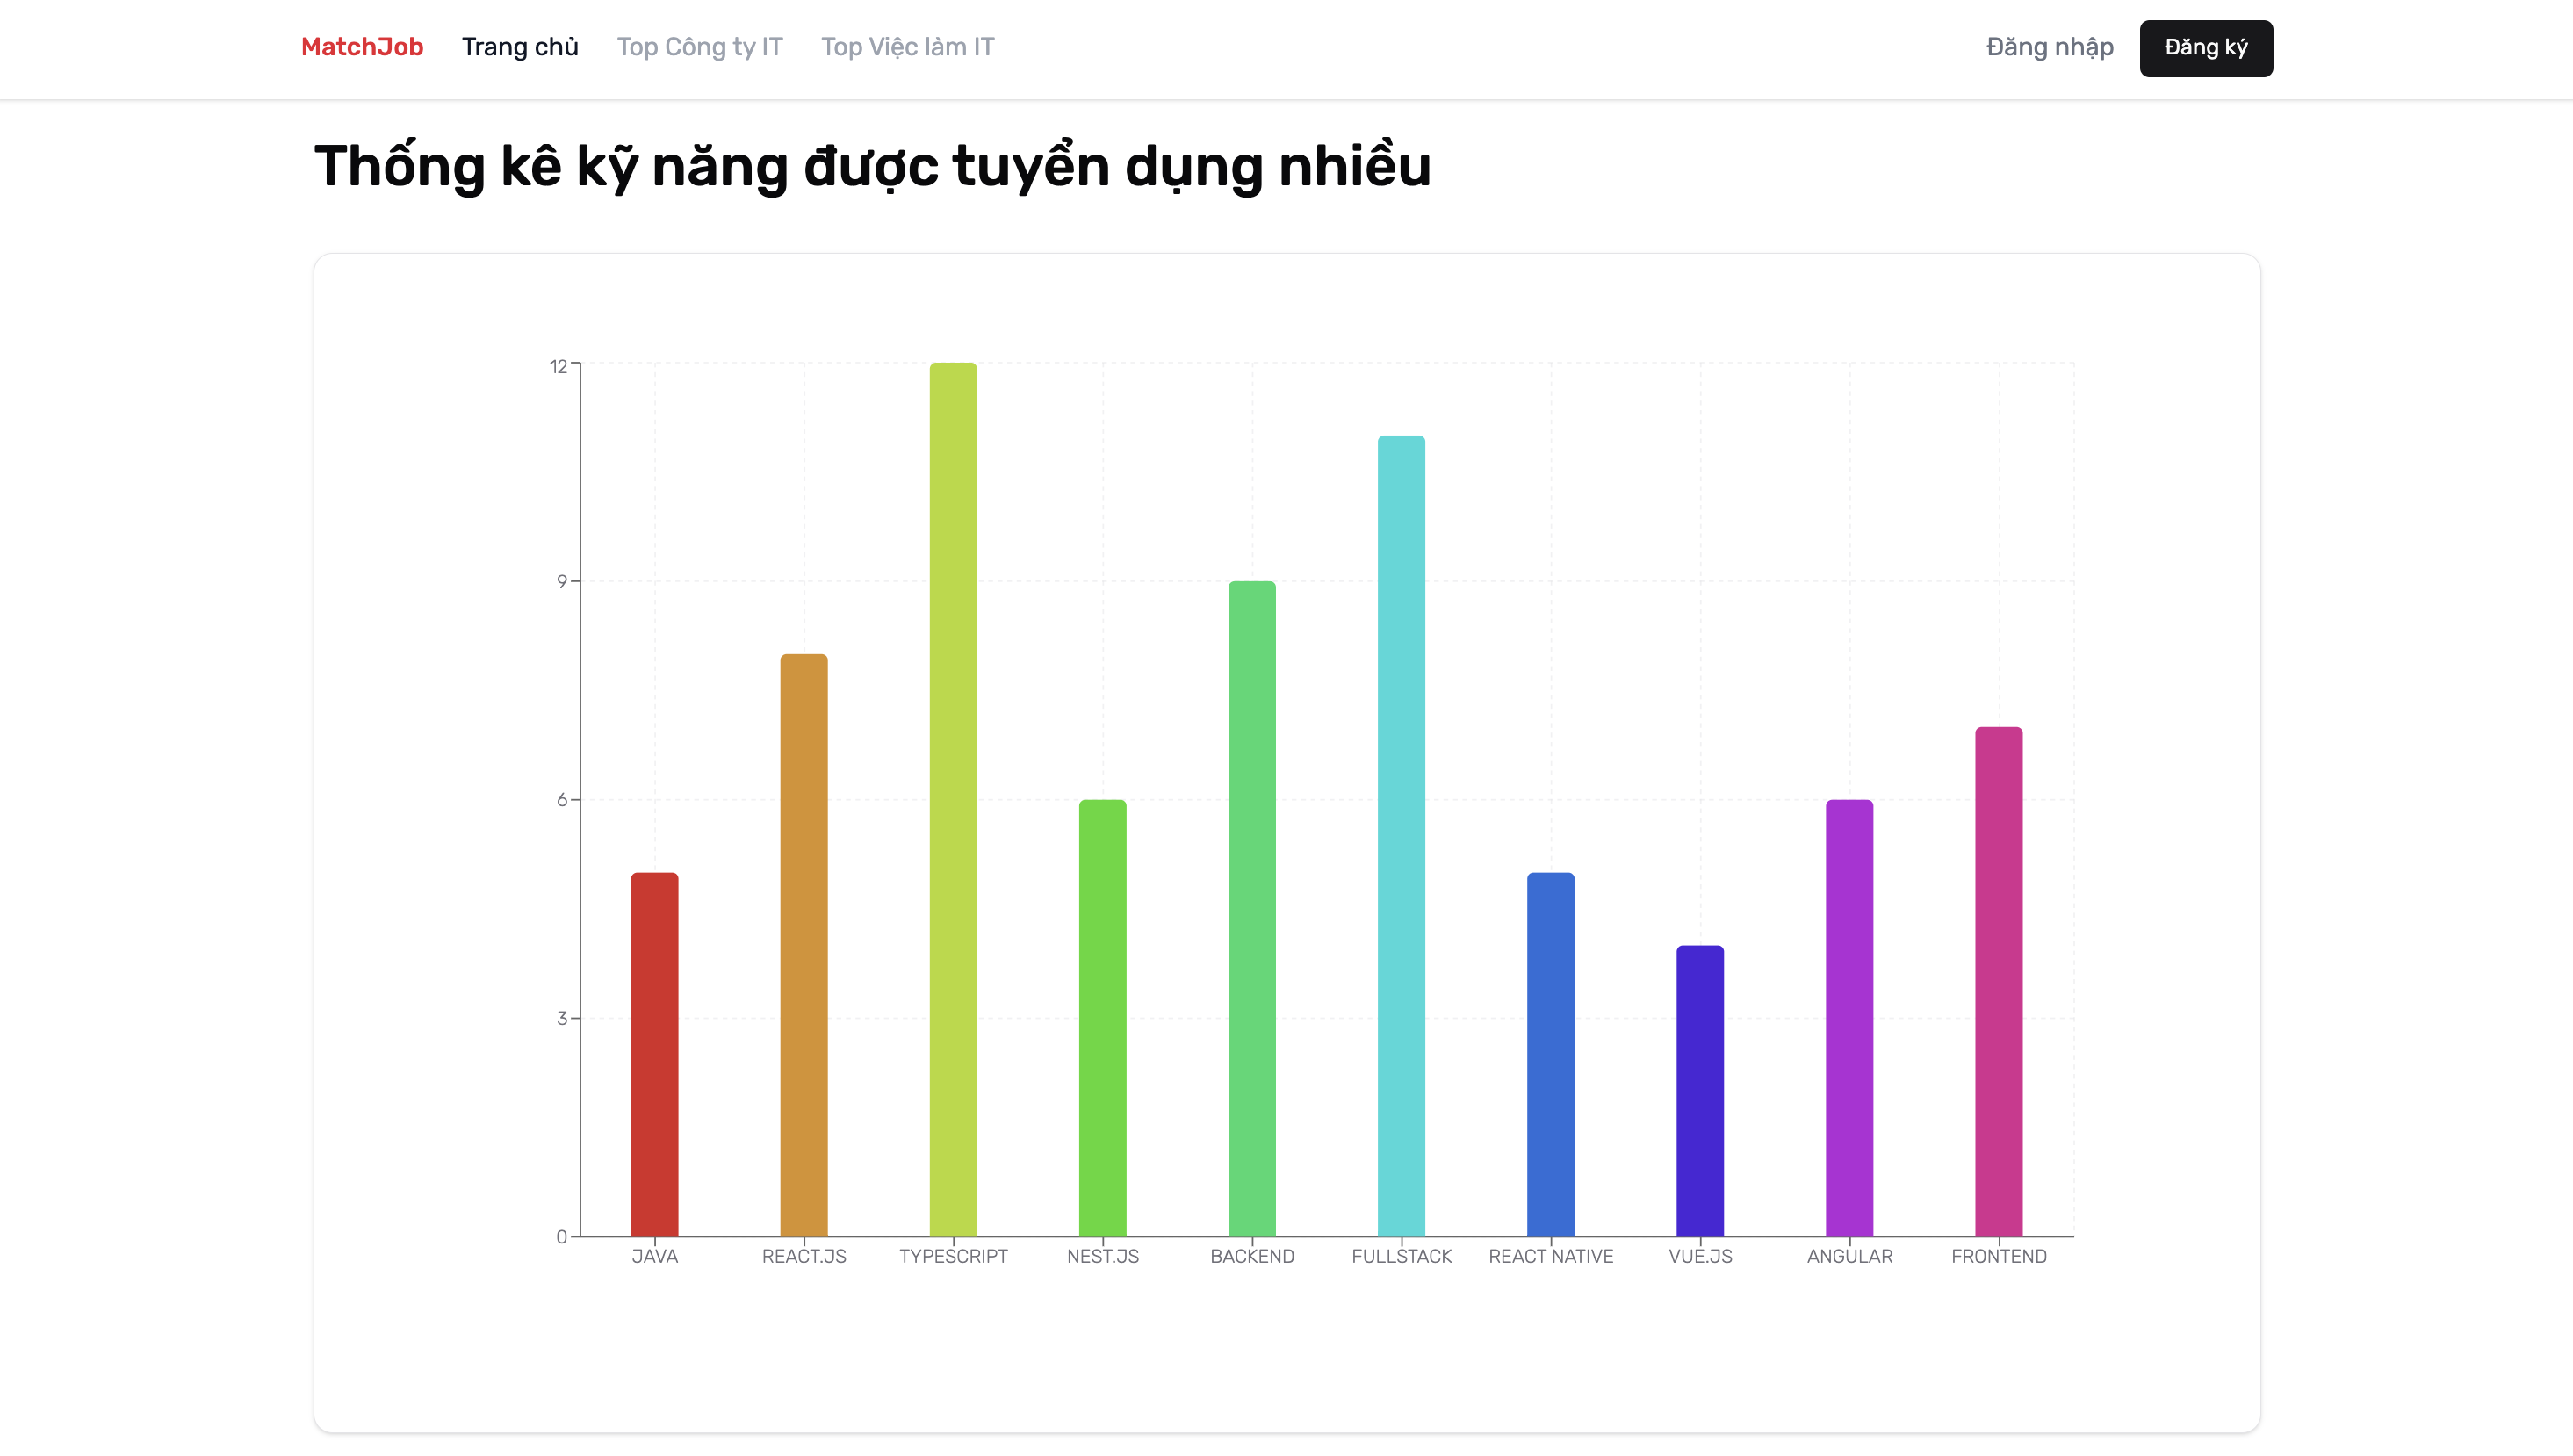
\includegraphics[width=\linewidth]{DBMS-Application/Images/user-screen-skill-stats.png}
    \caption{Trang chủ - Thống kê kỹ năng được tuyển dụng nhiều}
    \label{fig:enter-label}
\end{figure}

Truy vấn sử dụng: \textbf{Query with aggregation functions} - Sử dụng \texttt{\$sum} để tính tổng số công việc yêu cầu từng kỹ năng.

\begin{lstlisting}
const pipeline = [
  { $unwind: '$skills' },
  { $group: { _id: '$skills', total: { $sum: 1 } } },
  { $project: { skill: '$_id', total: 1, _id: 0 } },
];

return await this.db
  .collection('jobs')
  .aggregate(pipeline)
  .toArray();
\end{lstlisting}

Giải thích truy vấn:
\begin{itemize}
    \item \texttt{\$unwind}: Tách từng phần tử trong mảng skills của mỗi công việc thành các document riêng lẻ.
    \item \texttt{\$group}: Nhóm các document theo kỹ năng (skills) và đếm số lượng công việc yêu cầu kỹ năng đó bằng cách cộng dồn (\$sum: 1).
    \item \texttt{\$project}: Chọn các trường cần trả về, đổi tên \_id thành skill và bỏ trường \_id trong kết quả.
\end{itemize}

% \subsubsection{Giao diện người dùng - Danh sách/Chi tiết công ty}

Khi truy cập vào trang danh sách công ty, Front-end sẽ tự động fetch dữ liệu từ Backend thông qua một API tương tự như ở trang chủ: thực hiện phân trang để lấy lần lượt các công ty trong cơ sở dữ liệu dựa trên tham số \texttt{current} và \texttt{pageSize}.

\begin{figure}[H]
    \centering
    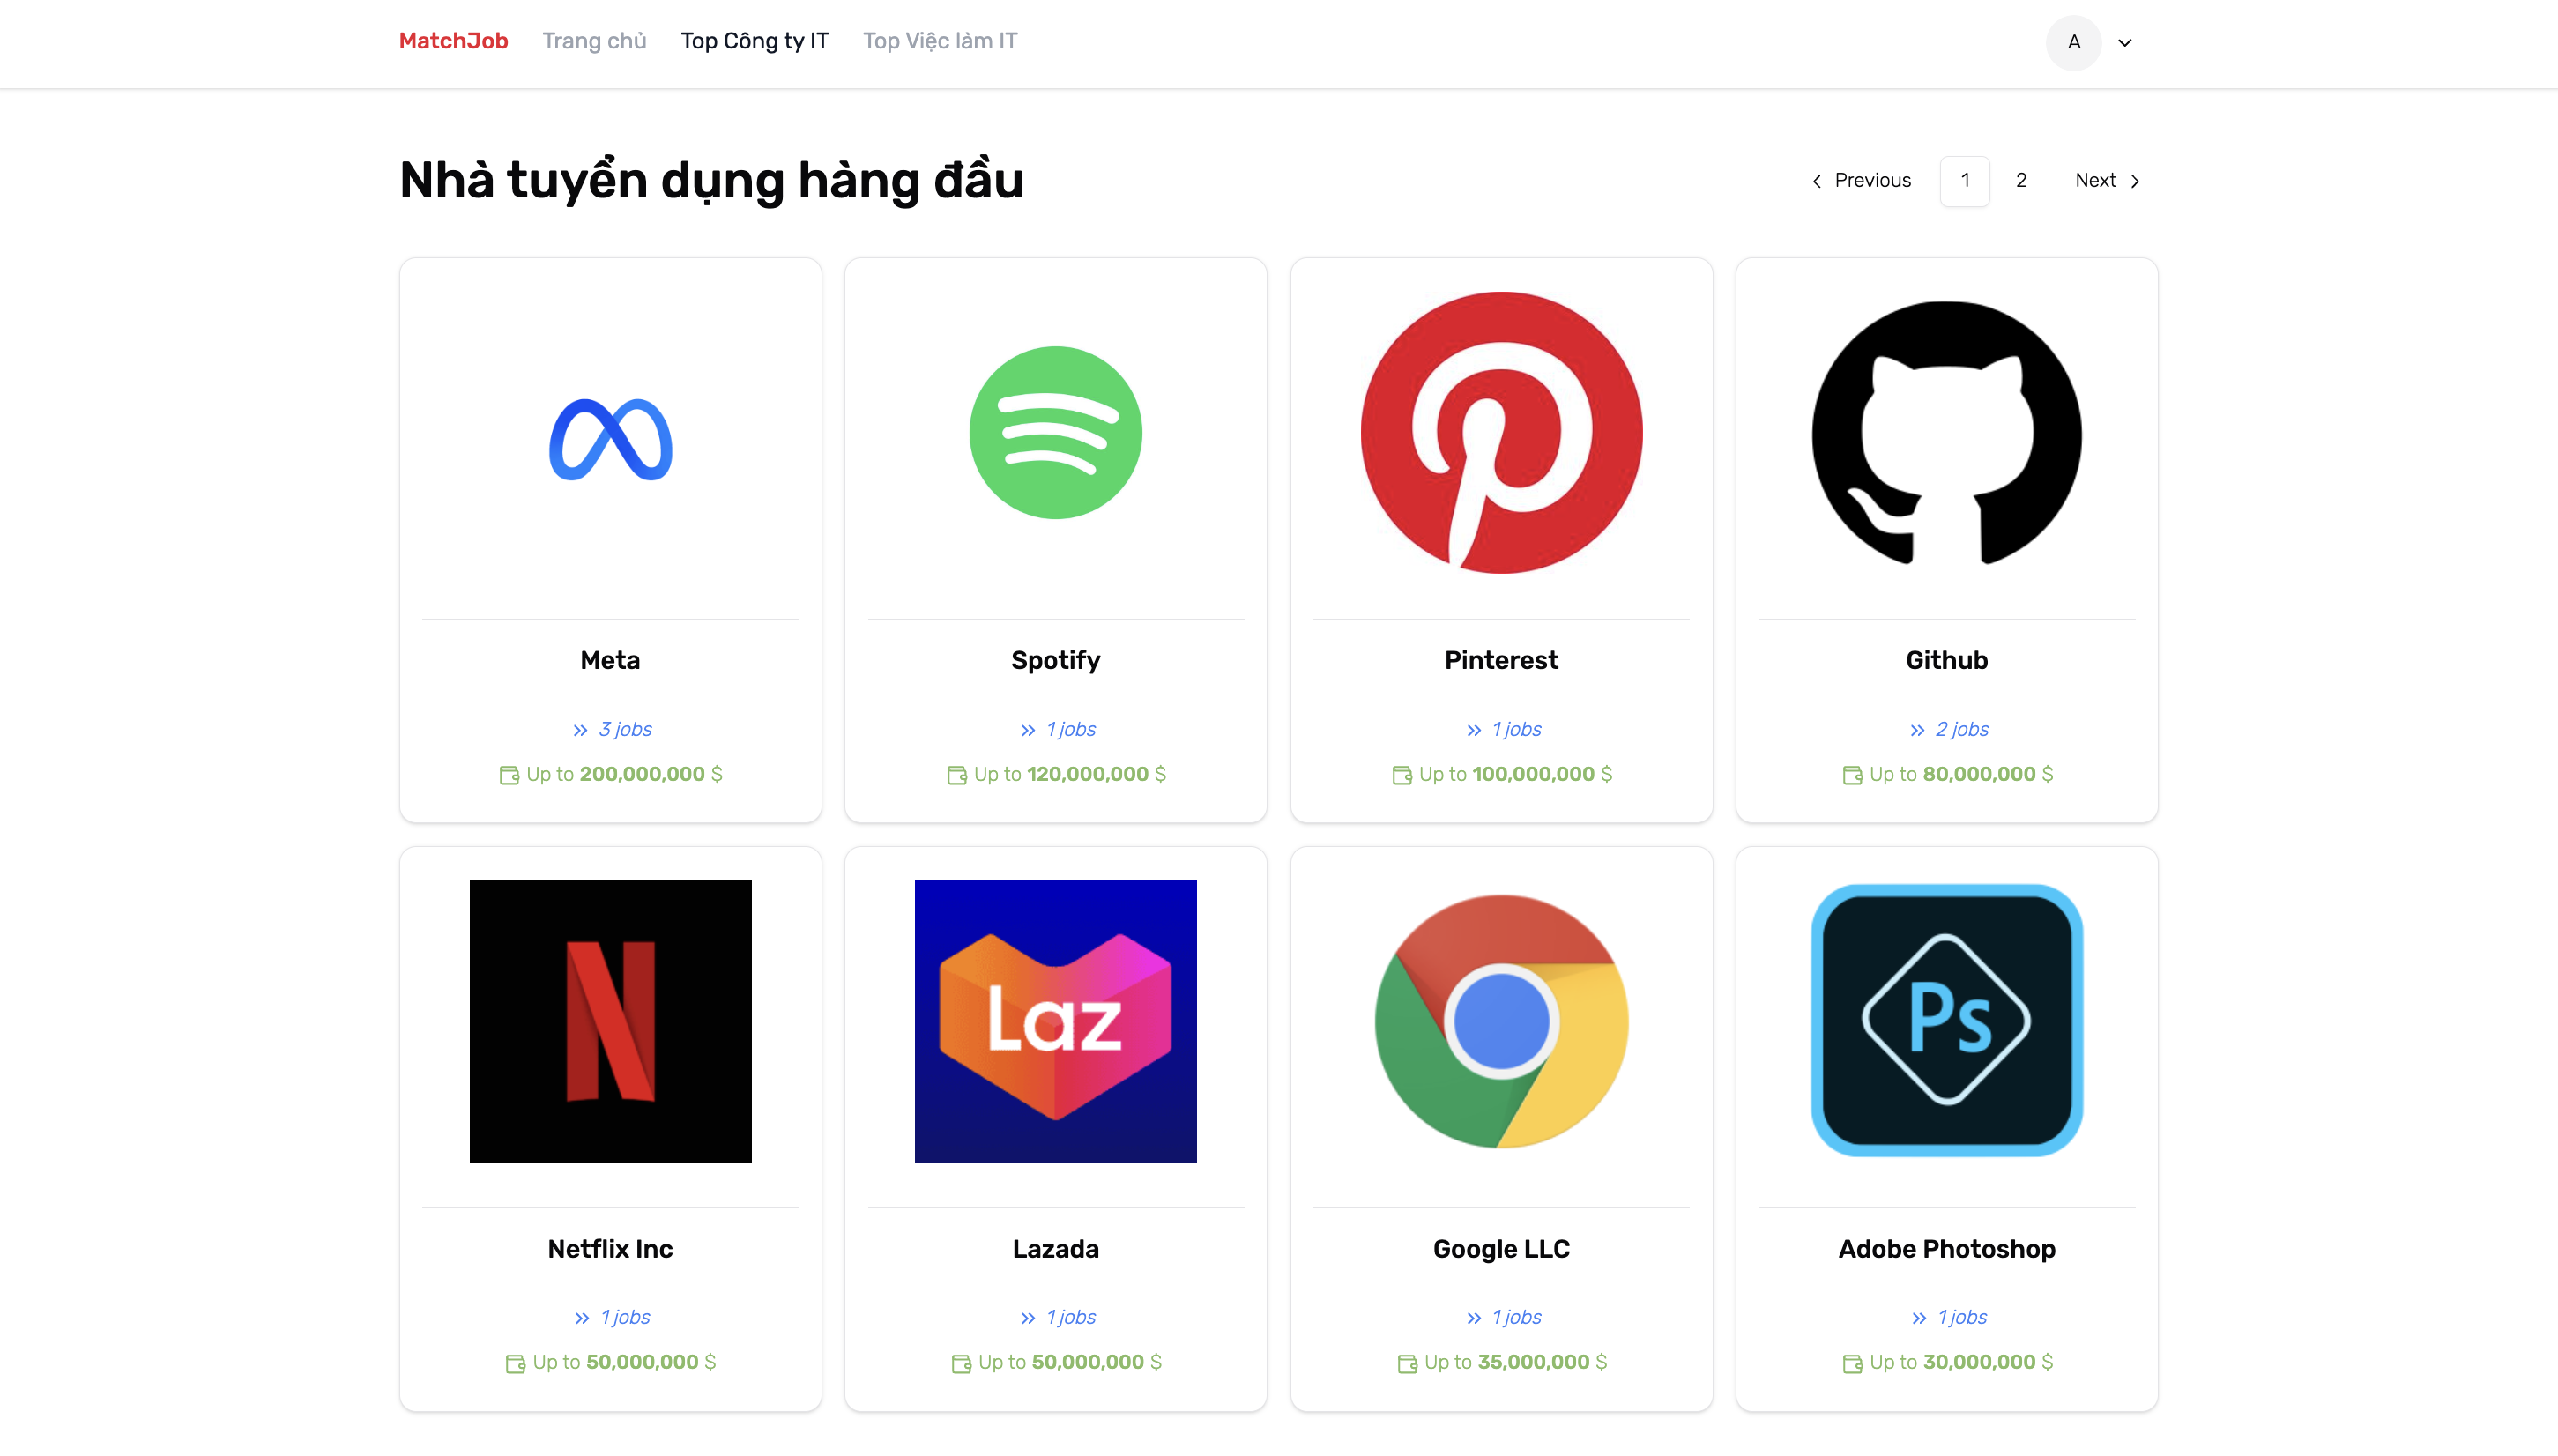
\includegraphics[width=\linewidth]{DBMS-Application/Images/list-company.png}
    \caption{Danh sách công ty}
    \label{fig:enter-label}
\end{figure}

Khi người dùng chọn 1 công ty trong danh sách, Front-end sẽ gửi yêu cầu đến API để lấy thông tin chi tiết của công ty đó và hiển thị lên giao diện người dùng:

\begin{figure}[H]
    \centering
    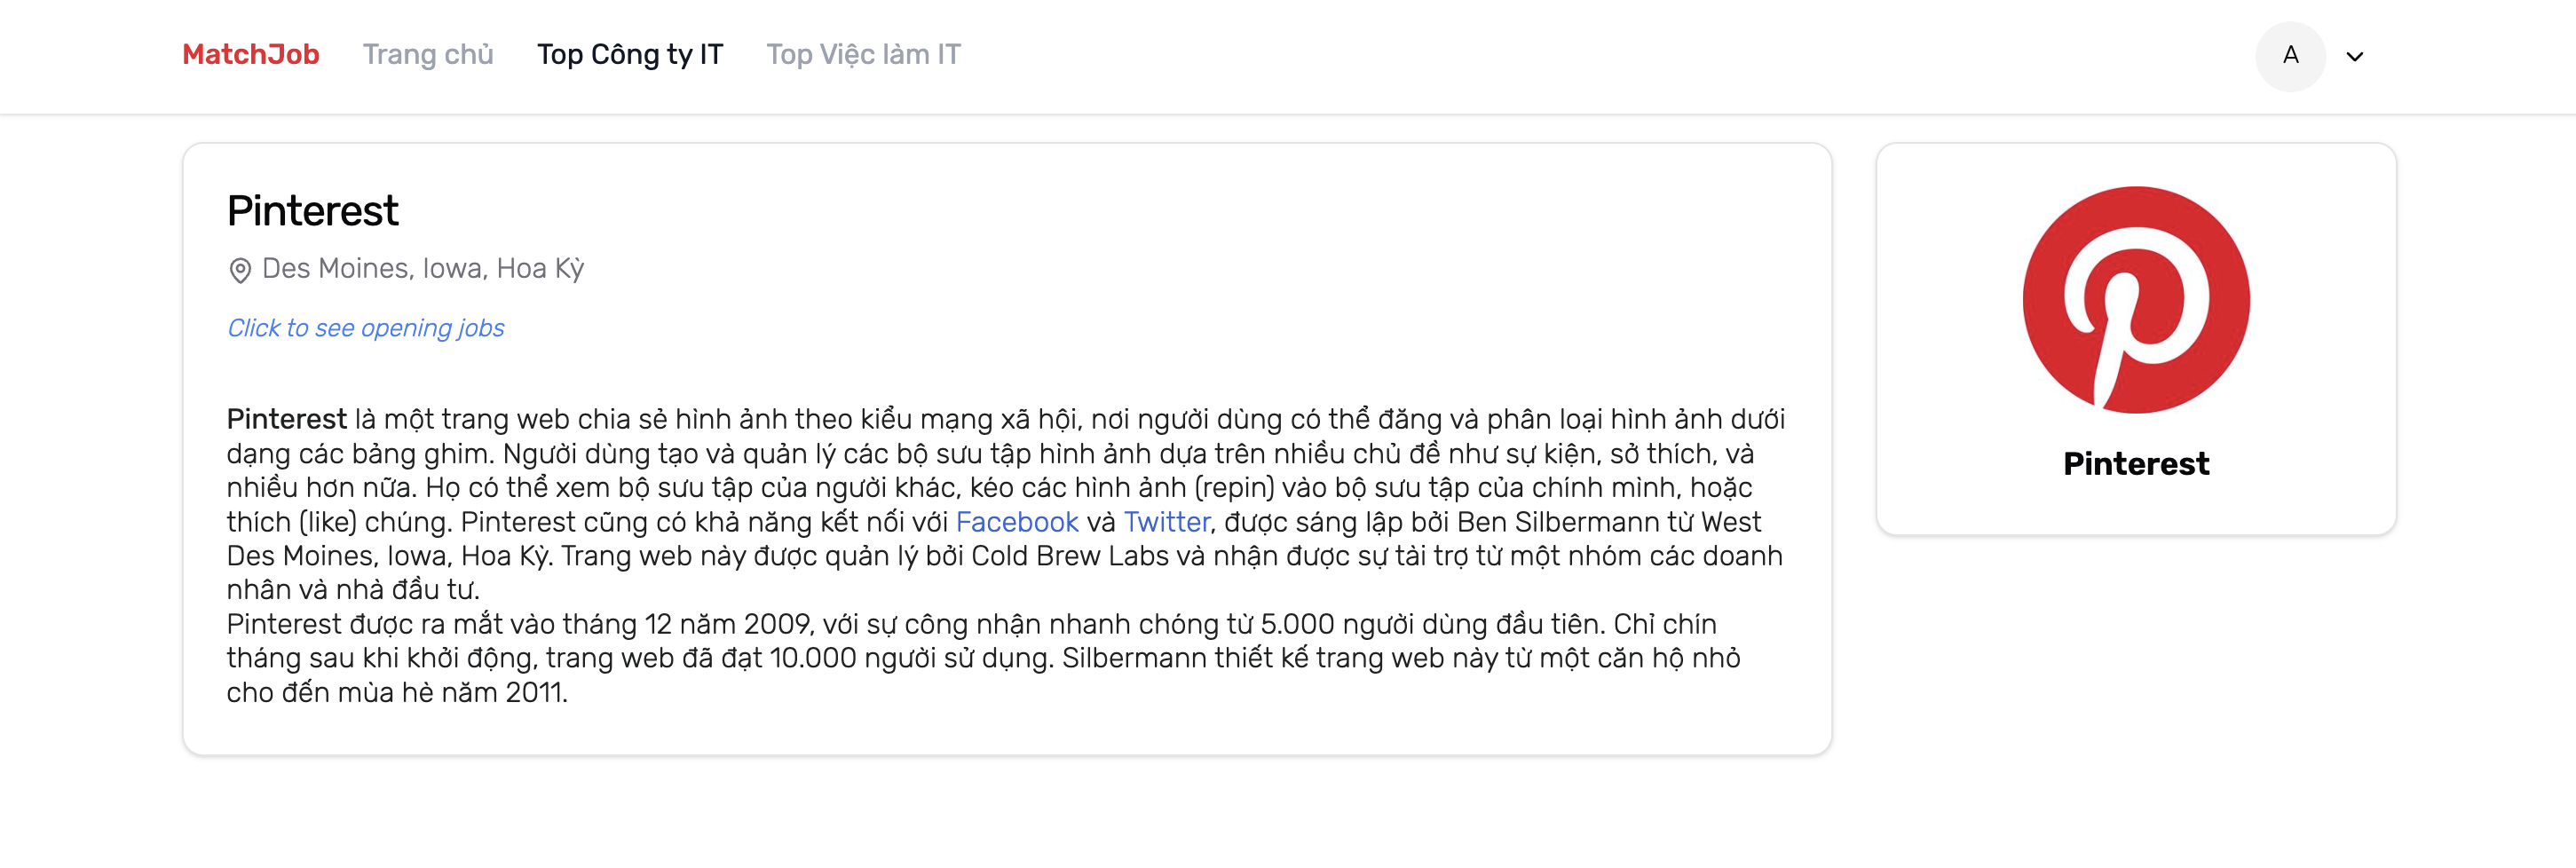
\includegraphics[width=\linewidth]{DBMS-Application/Images/company-detail.png}
    \caption{Thông tin chi tiết của công ty}
    \label{fig:enter-label}
\end{figure}

Truy vấn sử dụng: \textbf{Query with single condition} - Sử dụng điều kiện \texttt{\_id} để tìm công ty duy nhất

\begin{lstlisting}
return await this.db
  .collection('companies')
  .findOne({ _id: new ObjectId(id) }); // Chuyen id truyen vao thanh ObjectId, phu hop voi MongoDB
\end{lstlisting}

Ngoài ra, người dùng cũng có thể xem các công việc hiện đang được tuyển dụng của công ty này thông qua API lọc ra công việc của một công ty cụ thể (đã trình bày ở phần Trang chủ), hệ thống sẽ hiện lên 1 popup chứa các công việc của công ty hiện tại như sau:

\begin{figure}[H]
    \centering
    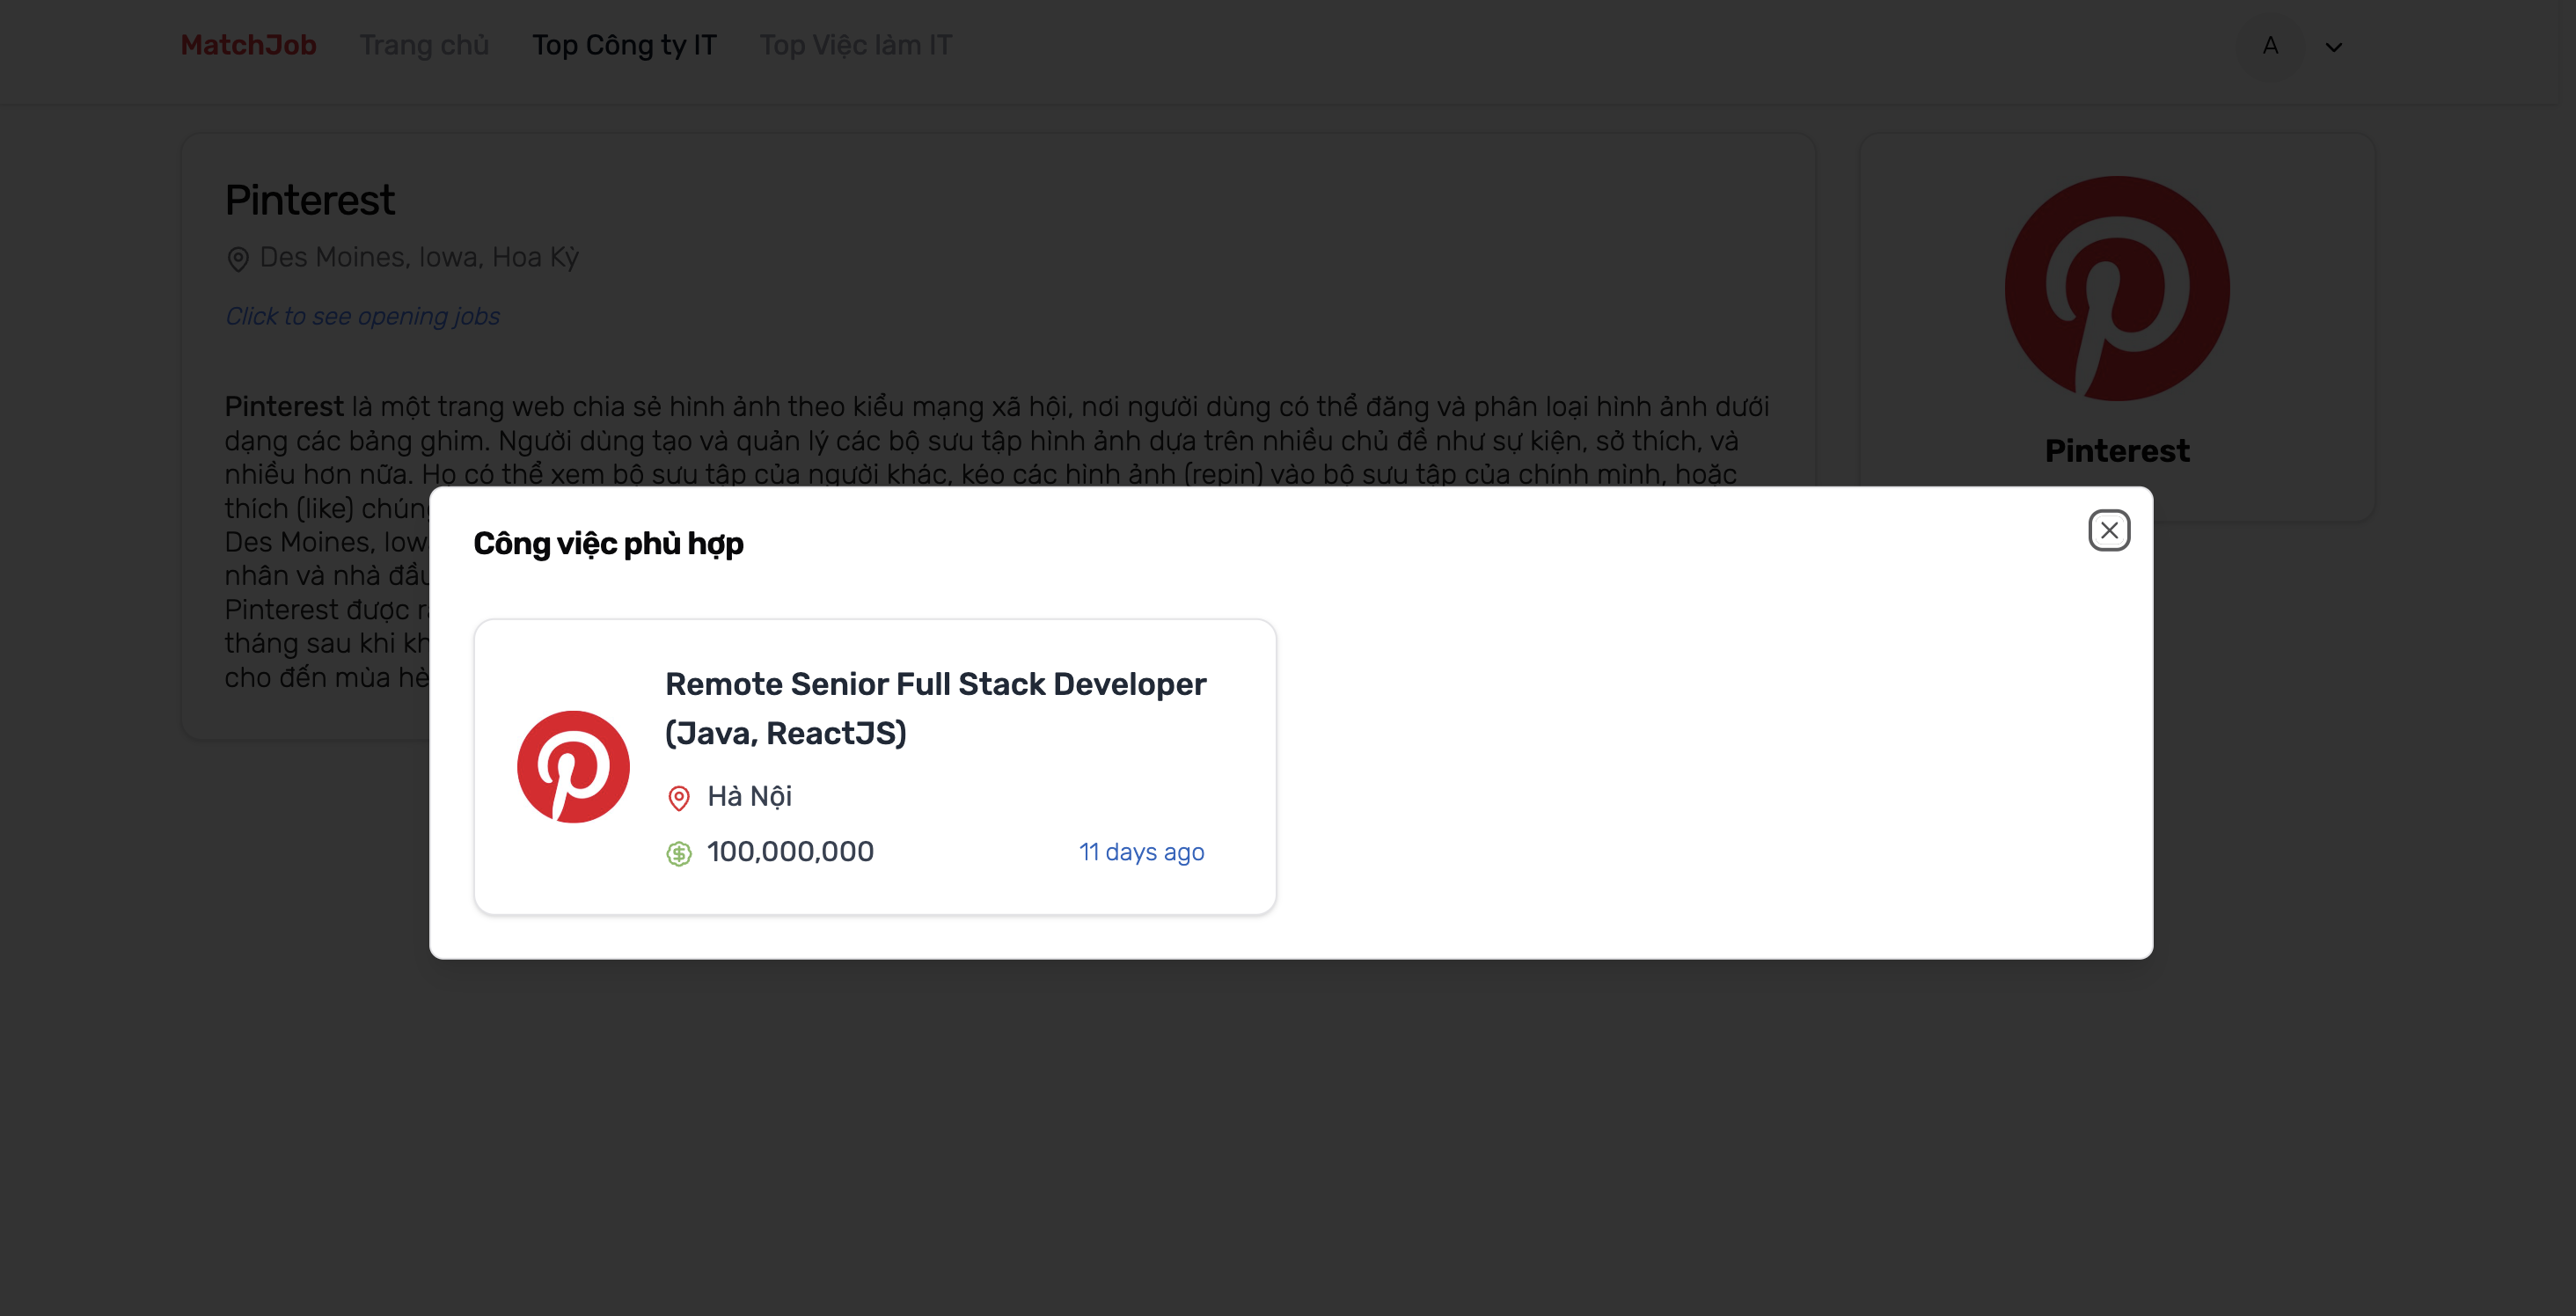
\includegraphics[width=\linewidth]{DBMS-Application/Images/modal-job-in-company-detail.png}
    \caption{Các công việc đang tuyển dụng của công ty cụ thể}
    \label{fig:enter-label}
\end{figure}




% \subsubsection{Giao diện người dùng - Danh sách/Chi tiết công việc}

Khi truy cập vào trang danh sách công việc tuyển dụng, Front-end sẽ tự động fetch dữ liệu từ Backend thông qua một API tương tự như ở trang chủ: thực hiện phân trang để lấy lần lượt các công việc trong cơ sở dữ liệu dựa trên tham số \texttt{current} và \texttt{pageSize}.

\begin{figure}[H]
    \centering
    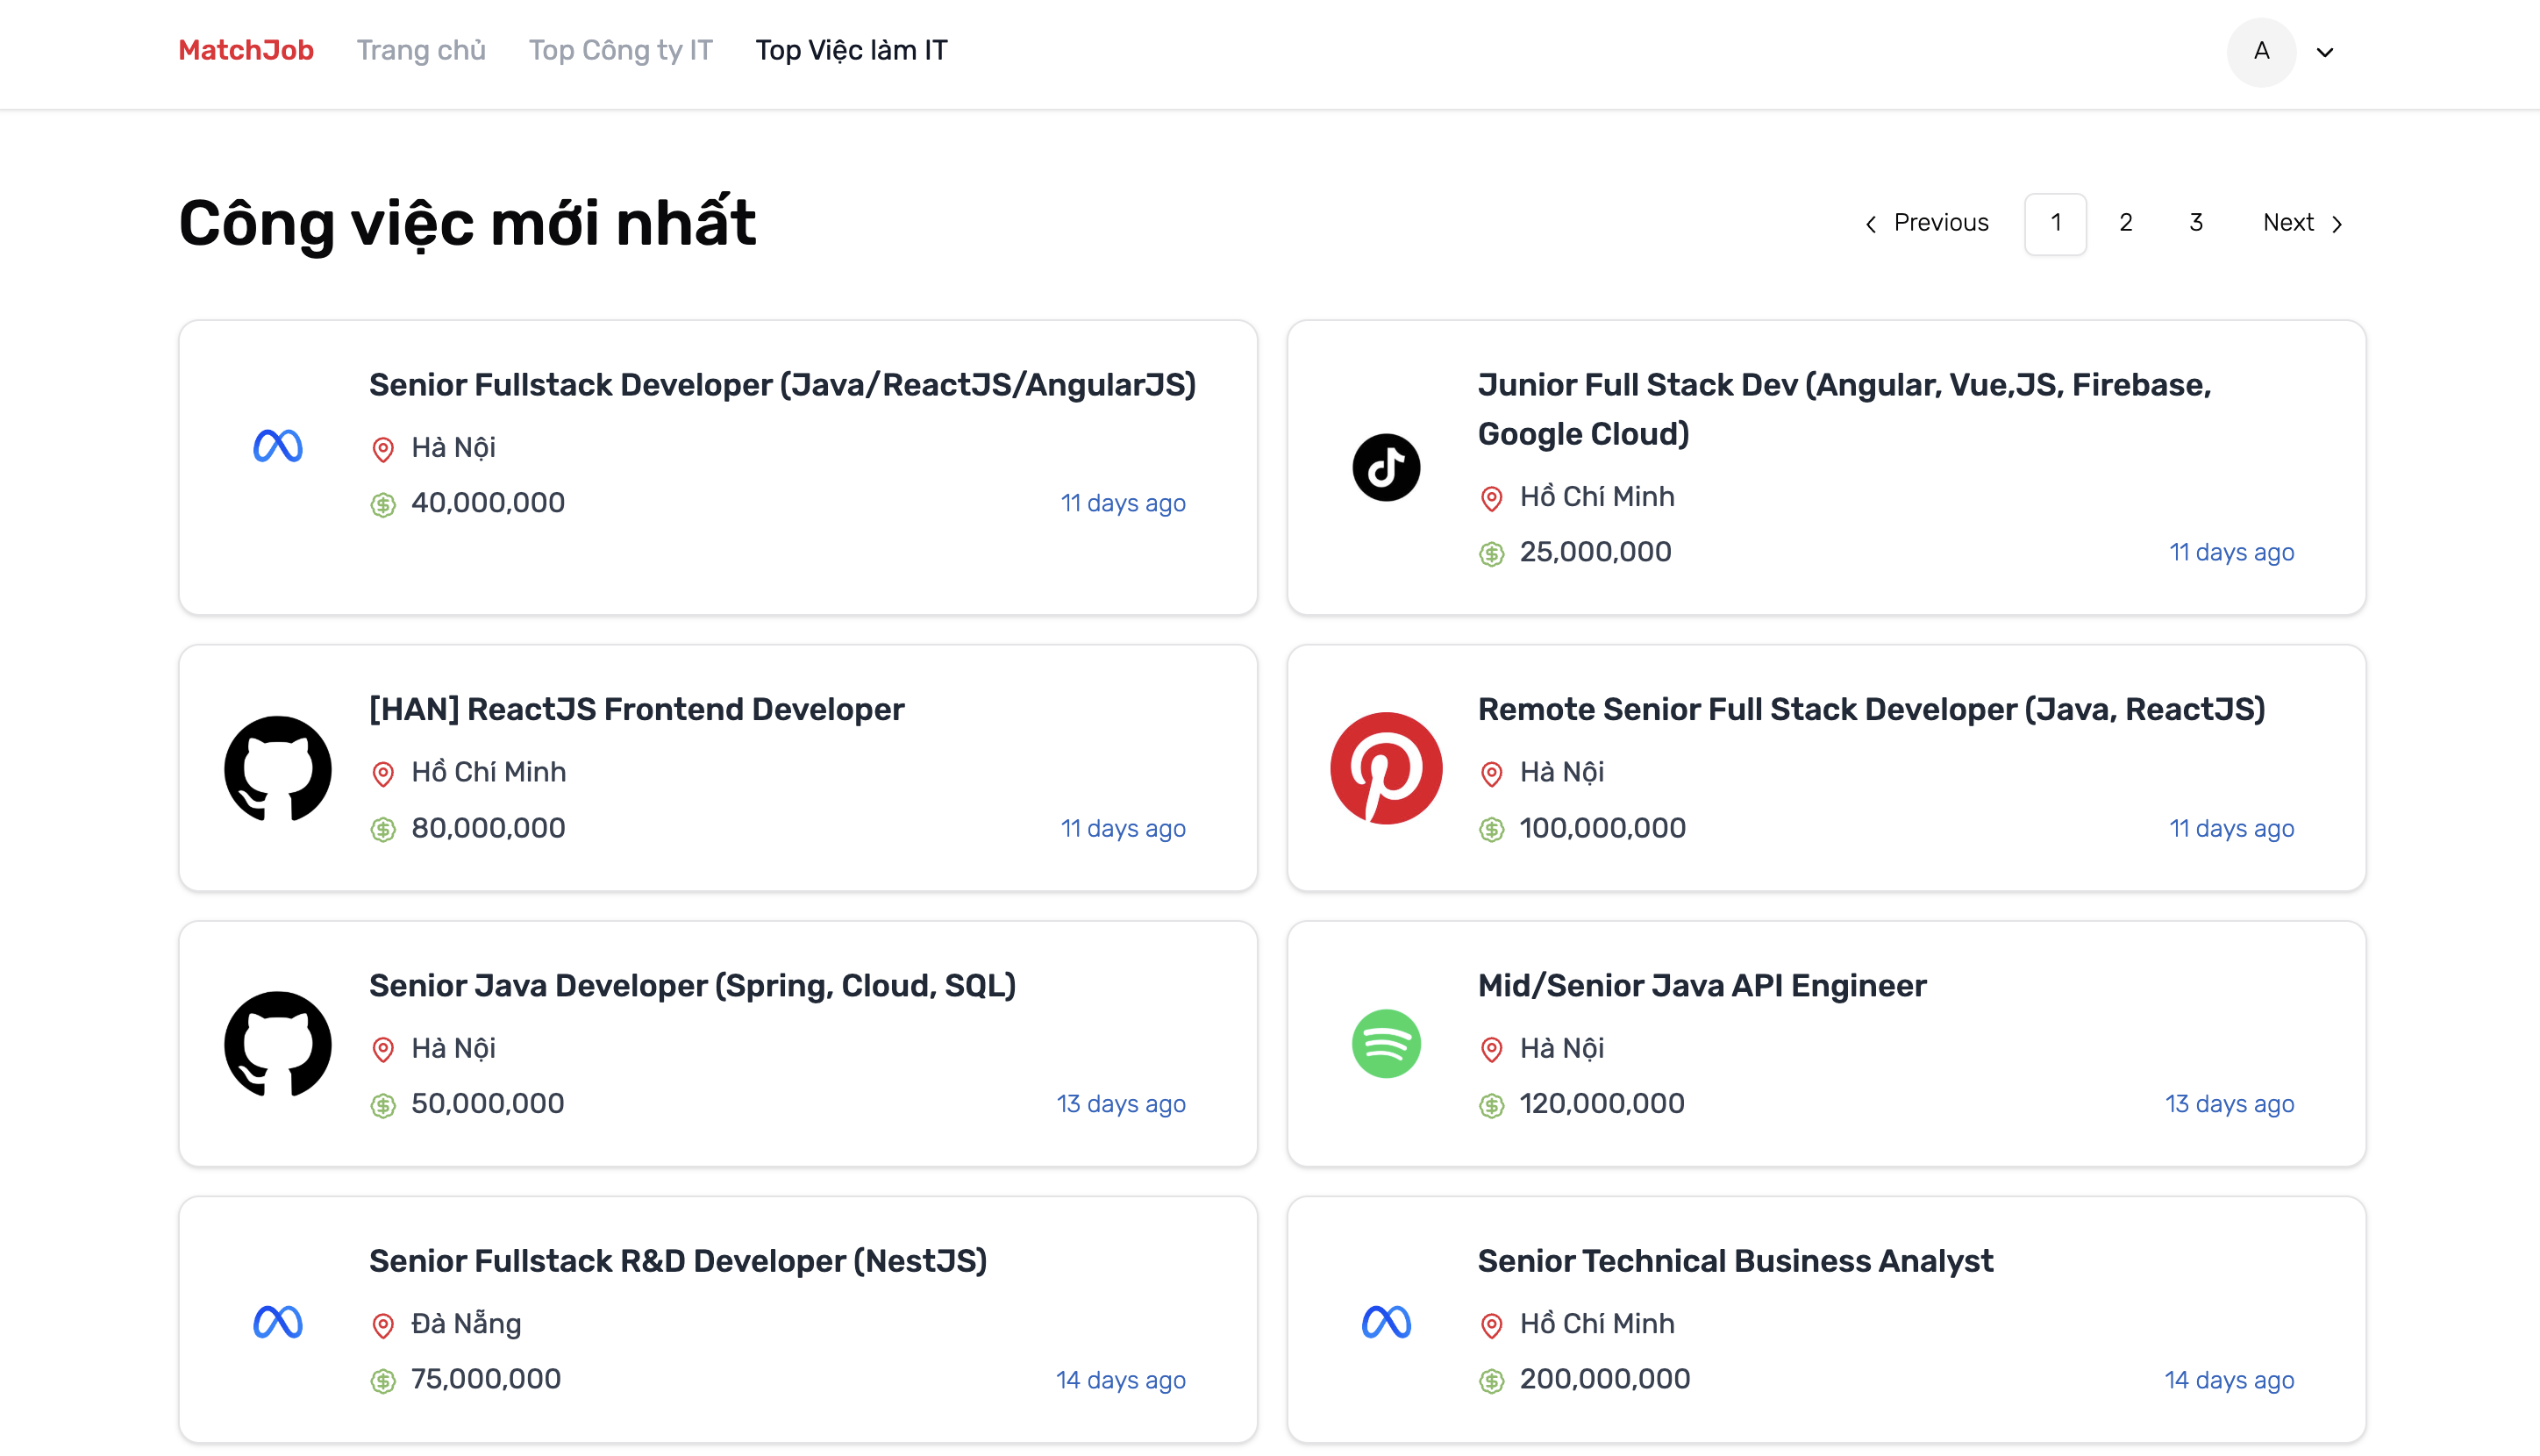
\includegraphics[width=\linewidth]{DBMS-Application/Images/list-job.png}
    \caption{Danh sách công việc đang được tuyển dụng}
\end{figure}

Và cũng như ở trang Danh sách công ty đã trình bày, người dùng cũng có thể chọn 1 công việc để xem chi tiết công việc đó:

\begin{figure}[H]
    \centering
    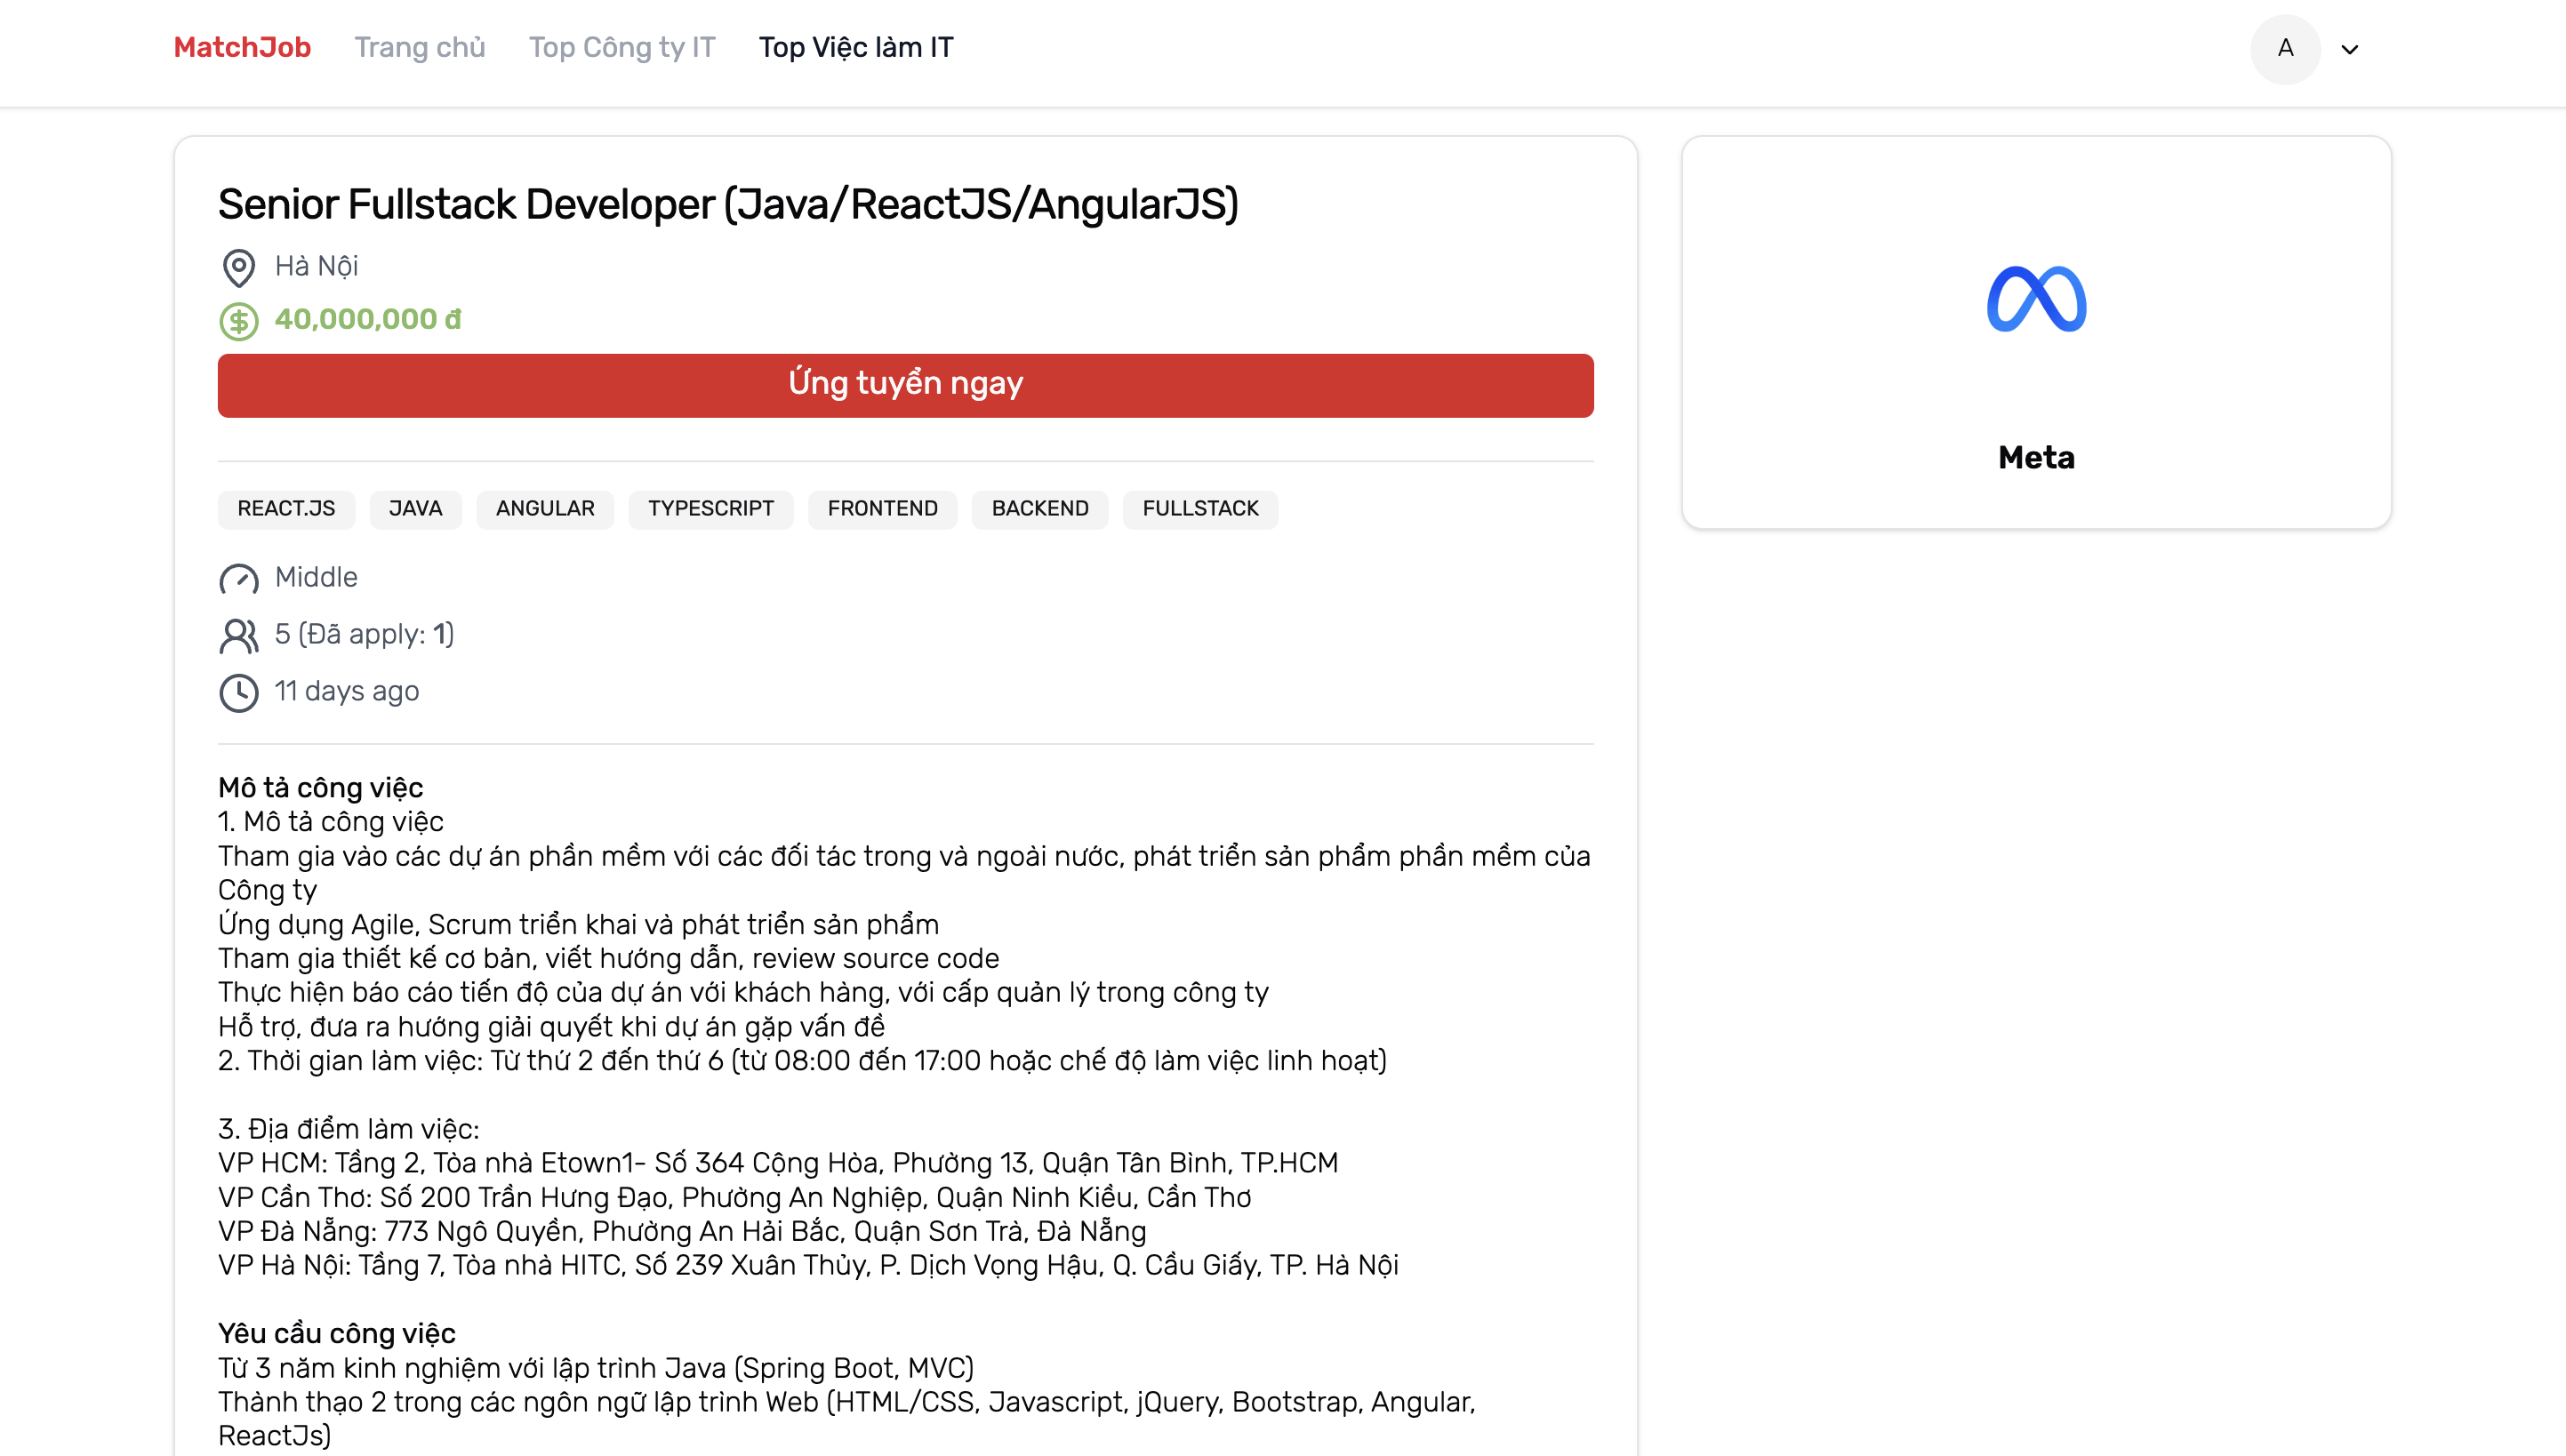
\includegraphics[width=\linewidth]{DBMS-Application/Images/job-detail.png}
    \caption{Danh sách công việc đang được tuyển dụng}
\end{figure}

Truy vấn sử dụng: \textbf{Query with single condition} - Sử dụng điều kiện \texttt{\_id} để tìm công việc duy nhất

\begin{lstlisting}
return await this.db
  .collection('jobs')
  .findOne({ _id: new ObjectId(id) });
\end{lstlisting}

Bên cạnh đó, hệ thống Front-end cũng tự động gửi yêu cầu thông qua API để lấy về số lượng hồ sơ đã nộp từ các ứng viên khác cho công việc hiện tại

\begin{figure}[H]
    \centering
    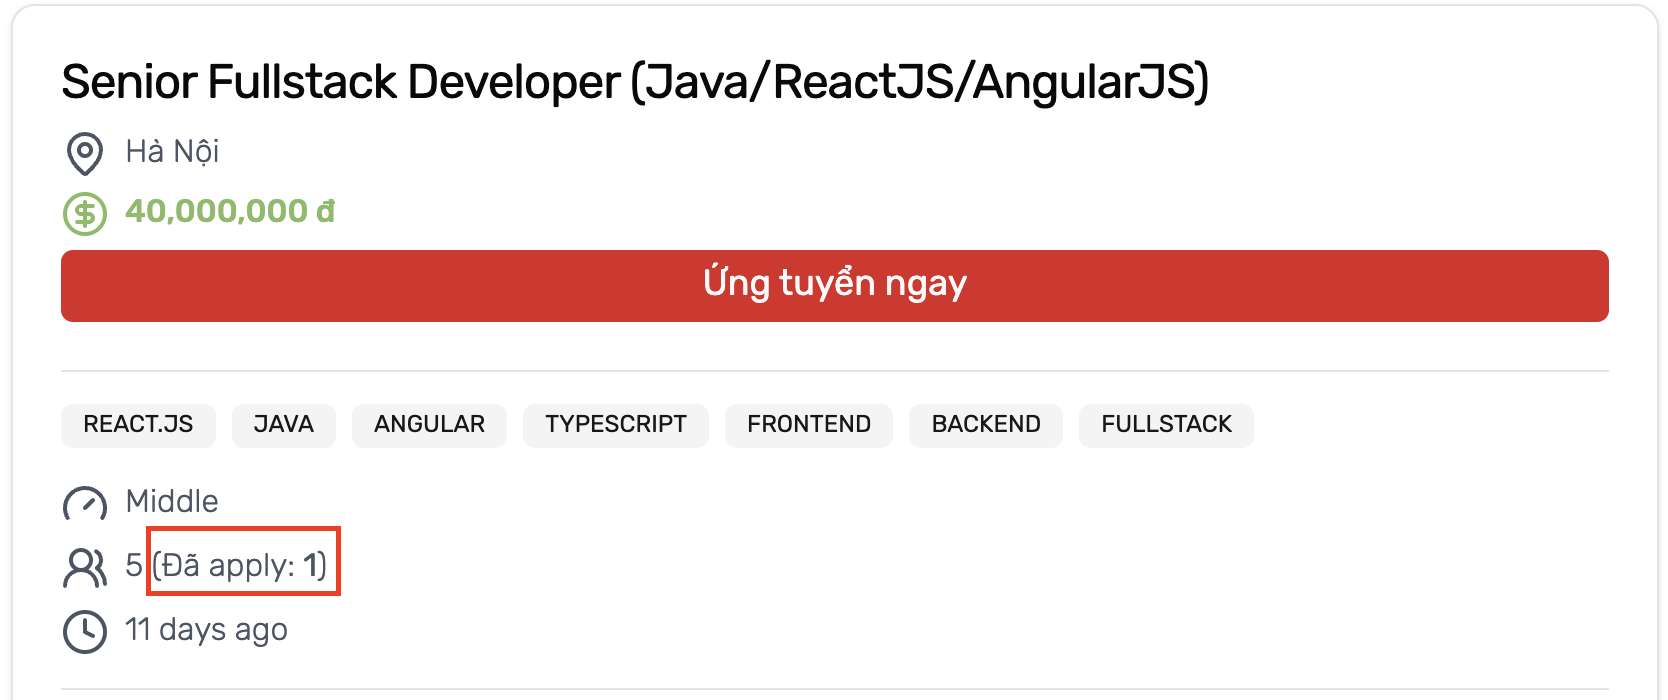
\includegraphics[width=.75\linewidth]{DBMS-Application/Images/number-resumes-apply.png}
    \caption{Số lượng hồ sơ đã được nộp cho công việc hiện tại}
\end{figure}

Truy vấn sử dụng:
\begin{itemize}
    \item \textbf{Query with single condition}: Sử dụng \texttt{\$match} để tìm một công việc cụ thể trong collection \textbf{jobs} dựa trên \texttt{\_id}
    
    \item \textbf{Query with join}: Thực hiện join thông qua \texttt{\$lookup} giữa collection \textbf{jobs} (\texttt{\_id}) và \textbf{resumes} (\texttt{jobId}) để lấy danh sách hồ sơ ứng tuyển của đến công việc đó

    \item \textbf{Query with aggregation functions}: Sử dụng \texttt{\$size} để tính tổng số lượng hồ sơ ứng tuyển của công việc
\end{itemize}

\begin{lstlisting}
const pipeline = [
  {
    $match: { _id: new ObjectId(id) }, // Tim job cu the thong qua _id
  },
  {
    $lookup: {
      from: 'resumes', // Join collection 'jobs' voi collection 'resumes'
      localField: '_id',
      foreignField: 'jobId',
      as: 'resumes',
    },
  },
  {
    $project: {
      _id: 1,
      totalResumes: { $size: '$resumes' }, // Dem so luong resumes da nop
    },
  },
];

const result = await this.db
  .collection('jobs')
  .aggregate(pipeline)
  .toArray();

return result[0];
\end{lstlisting}

Giải thích truy vấn:
\begin{itemize}
    \item \texttt{\$match}: Lọc công việc cụ thể từ collection \textbf{jobs} dựa trên \_id.
    \item \texttt{\$lookup}: Join với collection \textbf{resumes} để tìm các hồ sơ ứng tuyển có trường \texttt{jobId} trùng với \texttt{\_id} của công việc
    \item \texttt{\$project}: Trả về \texttt{\_id} của công việc và tổng số hồ sơ ứng tuyển (\texttt{totalResumes}) bằng cách sử dụng \texttt{\$size} để đếm số phần tử trong mảng resumes.
\end{itemize}

Cuối cùng, người dùng có thể upload (tạo) hồ sơ và apply cho công việc cụ thể:

\begin{figure}[H]
    \centering
    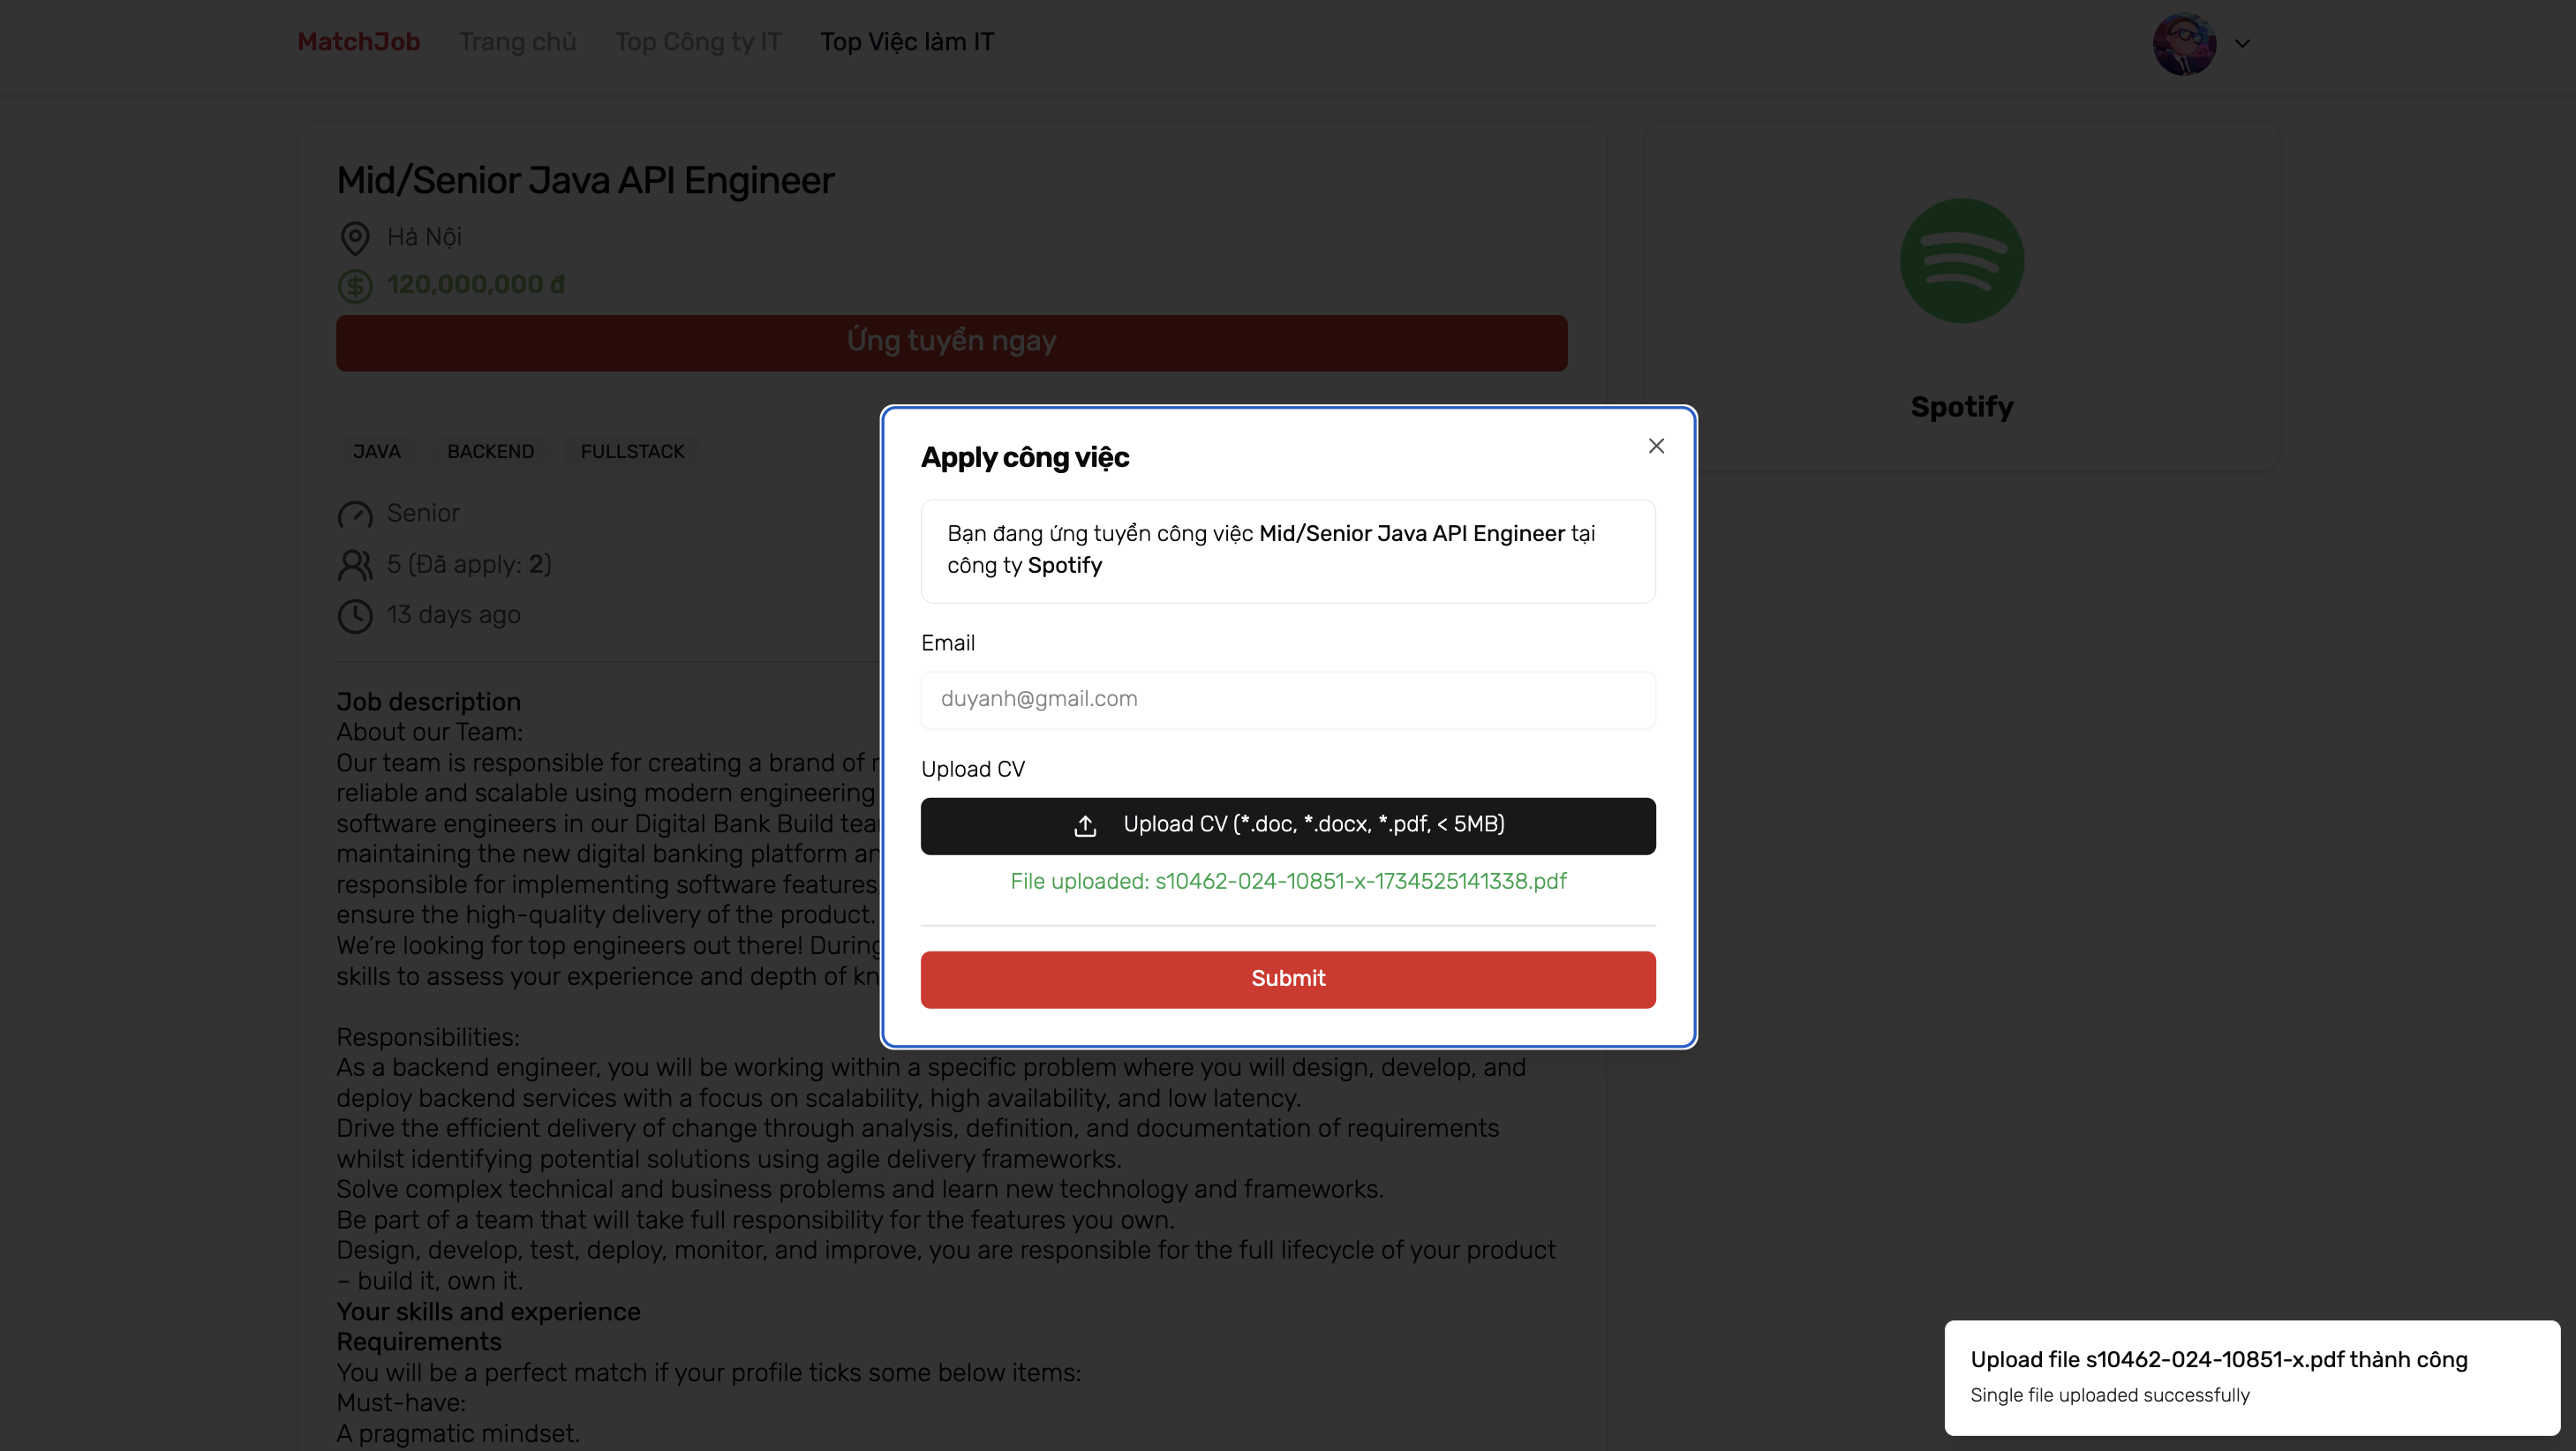
\includegraphics[width=\linewidth]{DBMS-Application/Images/modal-upload-cv.png}
    \caption{Số lượng hồ sơ đã được nộp cho công việc hiện tại}
\end{figure}

Truy vấn sử dụng: \textbf{Insert}

\begin{lstlisting}
const newResume = {
  url,
  companyId: new ObjectId(companyId),
  email,
  jobId: new ObjectId(jobId),
  userId: new ObjectId(_id),
  status: 'PENDING',
  createdAt: new Date(),
  updatedAt: new Date(),
};

const result = await this.db.collection('resumes').insertOne(newResume); // Them ho so ung tuyen moi vao database

return {
  _id: result.insertedId,
  createdAt: newResume.createdAt,
};

\end{lstlisting}


% \subsubsection{Giao diện người dùng - Danh sách hồ sơ đã ứng tuyển}

Người dùng có thể xem lại các hồ sơ ứng tuyển của họ cho từng công việc:

\begin{figure}[H]
    \centering
    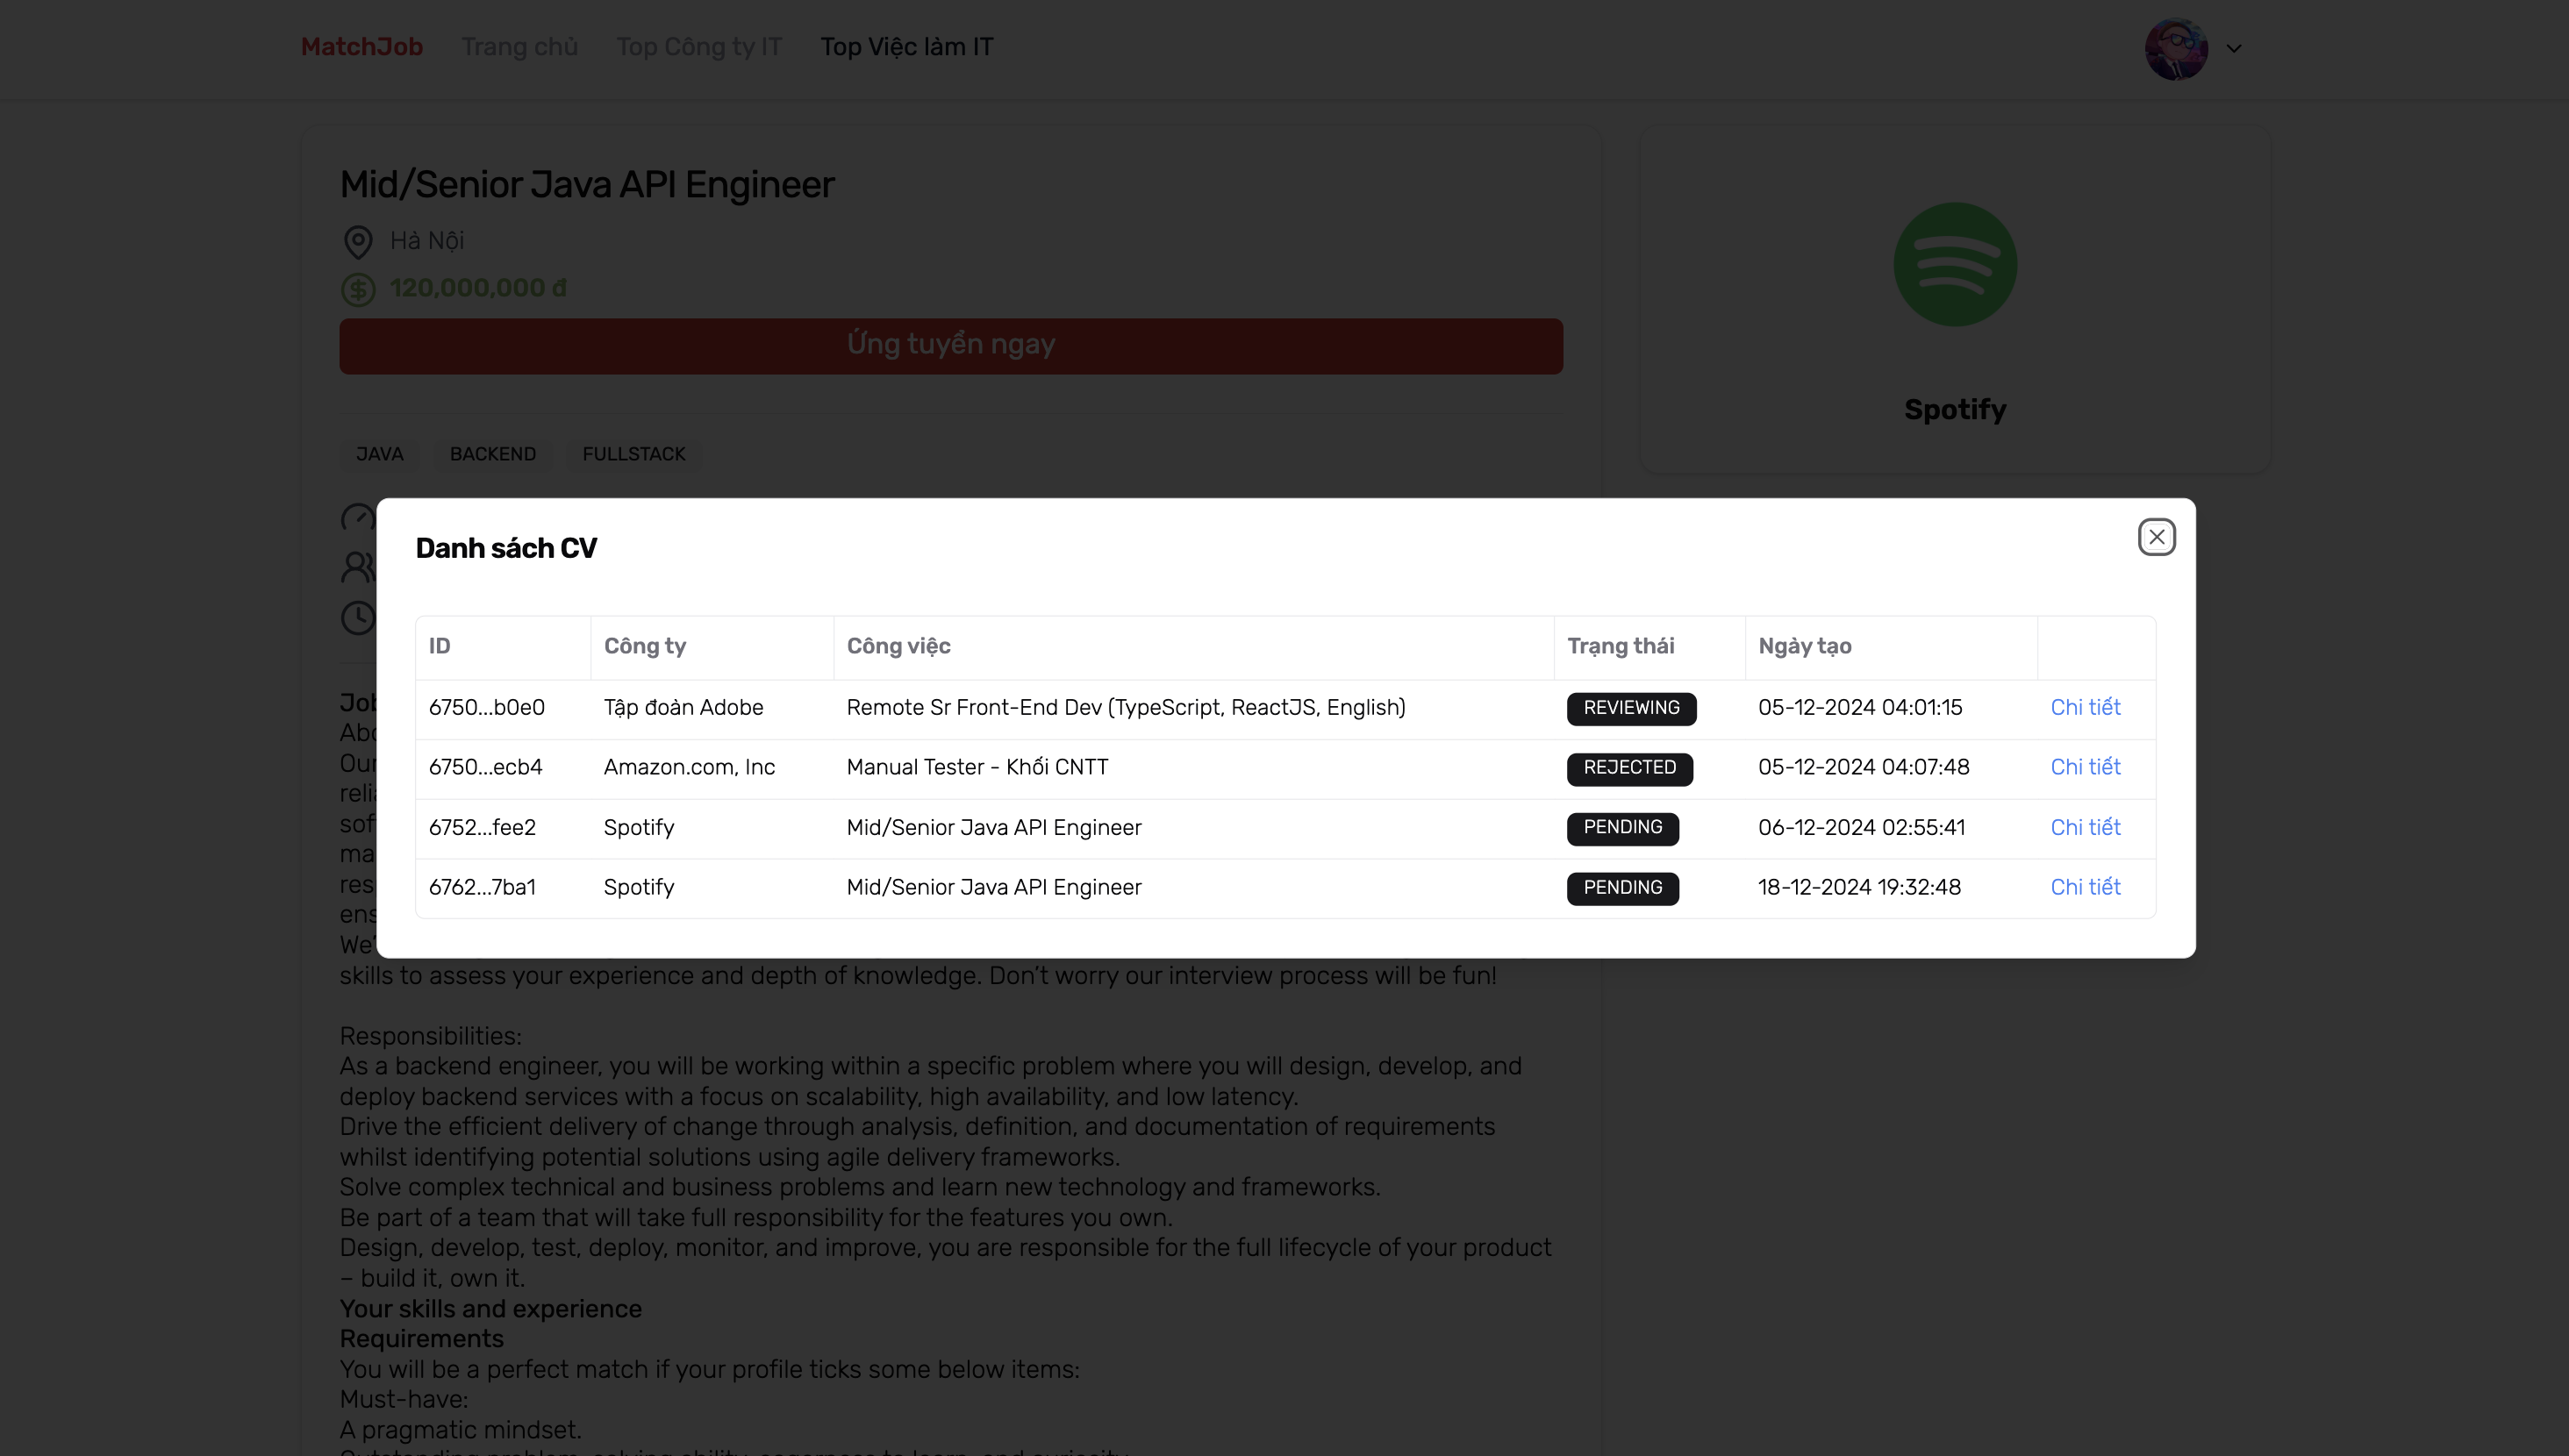
\includegraphics[width=\linewidth]{DBMS-Application/Images/modal-list-cv.png}
    \caption{Các hồ sơ đã được nộp của một người dùng}
\end{figure}

Truy vấn sử dụng:
\begin{itemize}
    \item \textbf{Query with join}: Sử dụng \texttt{\$lookup} để liên kết dữ liệu giữa hai collection \textbf{users} và \textbf{resumes}

    \item \textbf{Query with single condition}: Sử dụng \texttt{\$match} để lọc hồ sơ của của người dùng có \texttt{\_id}
\end{itemize}

\begin{lstlisting}
const result = await this.db
  .collection('users')
  .aggregate([
    {
      $lookup: {
        from: 'resumes',
        localField: '_id',
        foreignField: 'userId',
        as: 'userResumes',
      },
    },
    {
      $match: {
        _id: new ObjectId(user._id),
      },
    },
    {
      $project: {
        userResumes: 1,
      },
    },
  ])
  .toArray();

const resumes = result.length > 0 ? result[0].userResumes : [];
return resumes;
\end{lstlisting}

Giải thích truy vấn:
\begin{itemize}
    \item \texttt{\$lookup}: Thực hiện join giữa collection \textbf{users} và collection \textbf{resumes} để lấy tất cả các hồ sơ ứng tuyển của người dùng (\texttt{userId}) tương ứng với \texttt{\_id} của user.
    \item \texttt{\$match}: Lọc để chỉ lấy hồ sơ ứng tuyển của người dùng có \texttt{\_id} trùng với ID của user được truyền vào (\texttt{user.\_id}).
    \item \texttt{\$project}: Chỉ giữ lại trường \texttt{userResumes} trong kết quả trả về, ẩn các trường khác.
\end{itemize}

Truy vấn trả về mảng các hồ sơ ứng tuyển (\texttt{userResumes}) của người dùng (trả về mảng rỗng trong trường hợp người dùng chưa tải lên hồ sơ ứng tuyển nào)

% \subsubsection{Giao diện Admin - Quản lý công việc}

Trang quản lý công việc được thiết kế để hiển thị danh sách toàn bộ các công việc hiện có trong hệ thống, phục vụ việc quản lý, chỉnh sửa hoặc xóa công việc. Dữ liệu cũng được lấy từ Backend thông qua API theo cơ chế phân trang tương tự như các phần trước, giúp tối ưu hóa hiệu suất và hiển thị mượt mà, đặc biệt khi số lượng công việc lớn.

\begin{figure}[H]
    \centering
    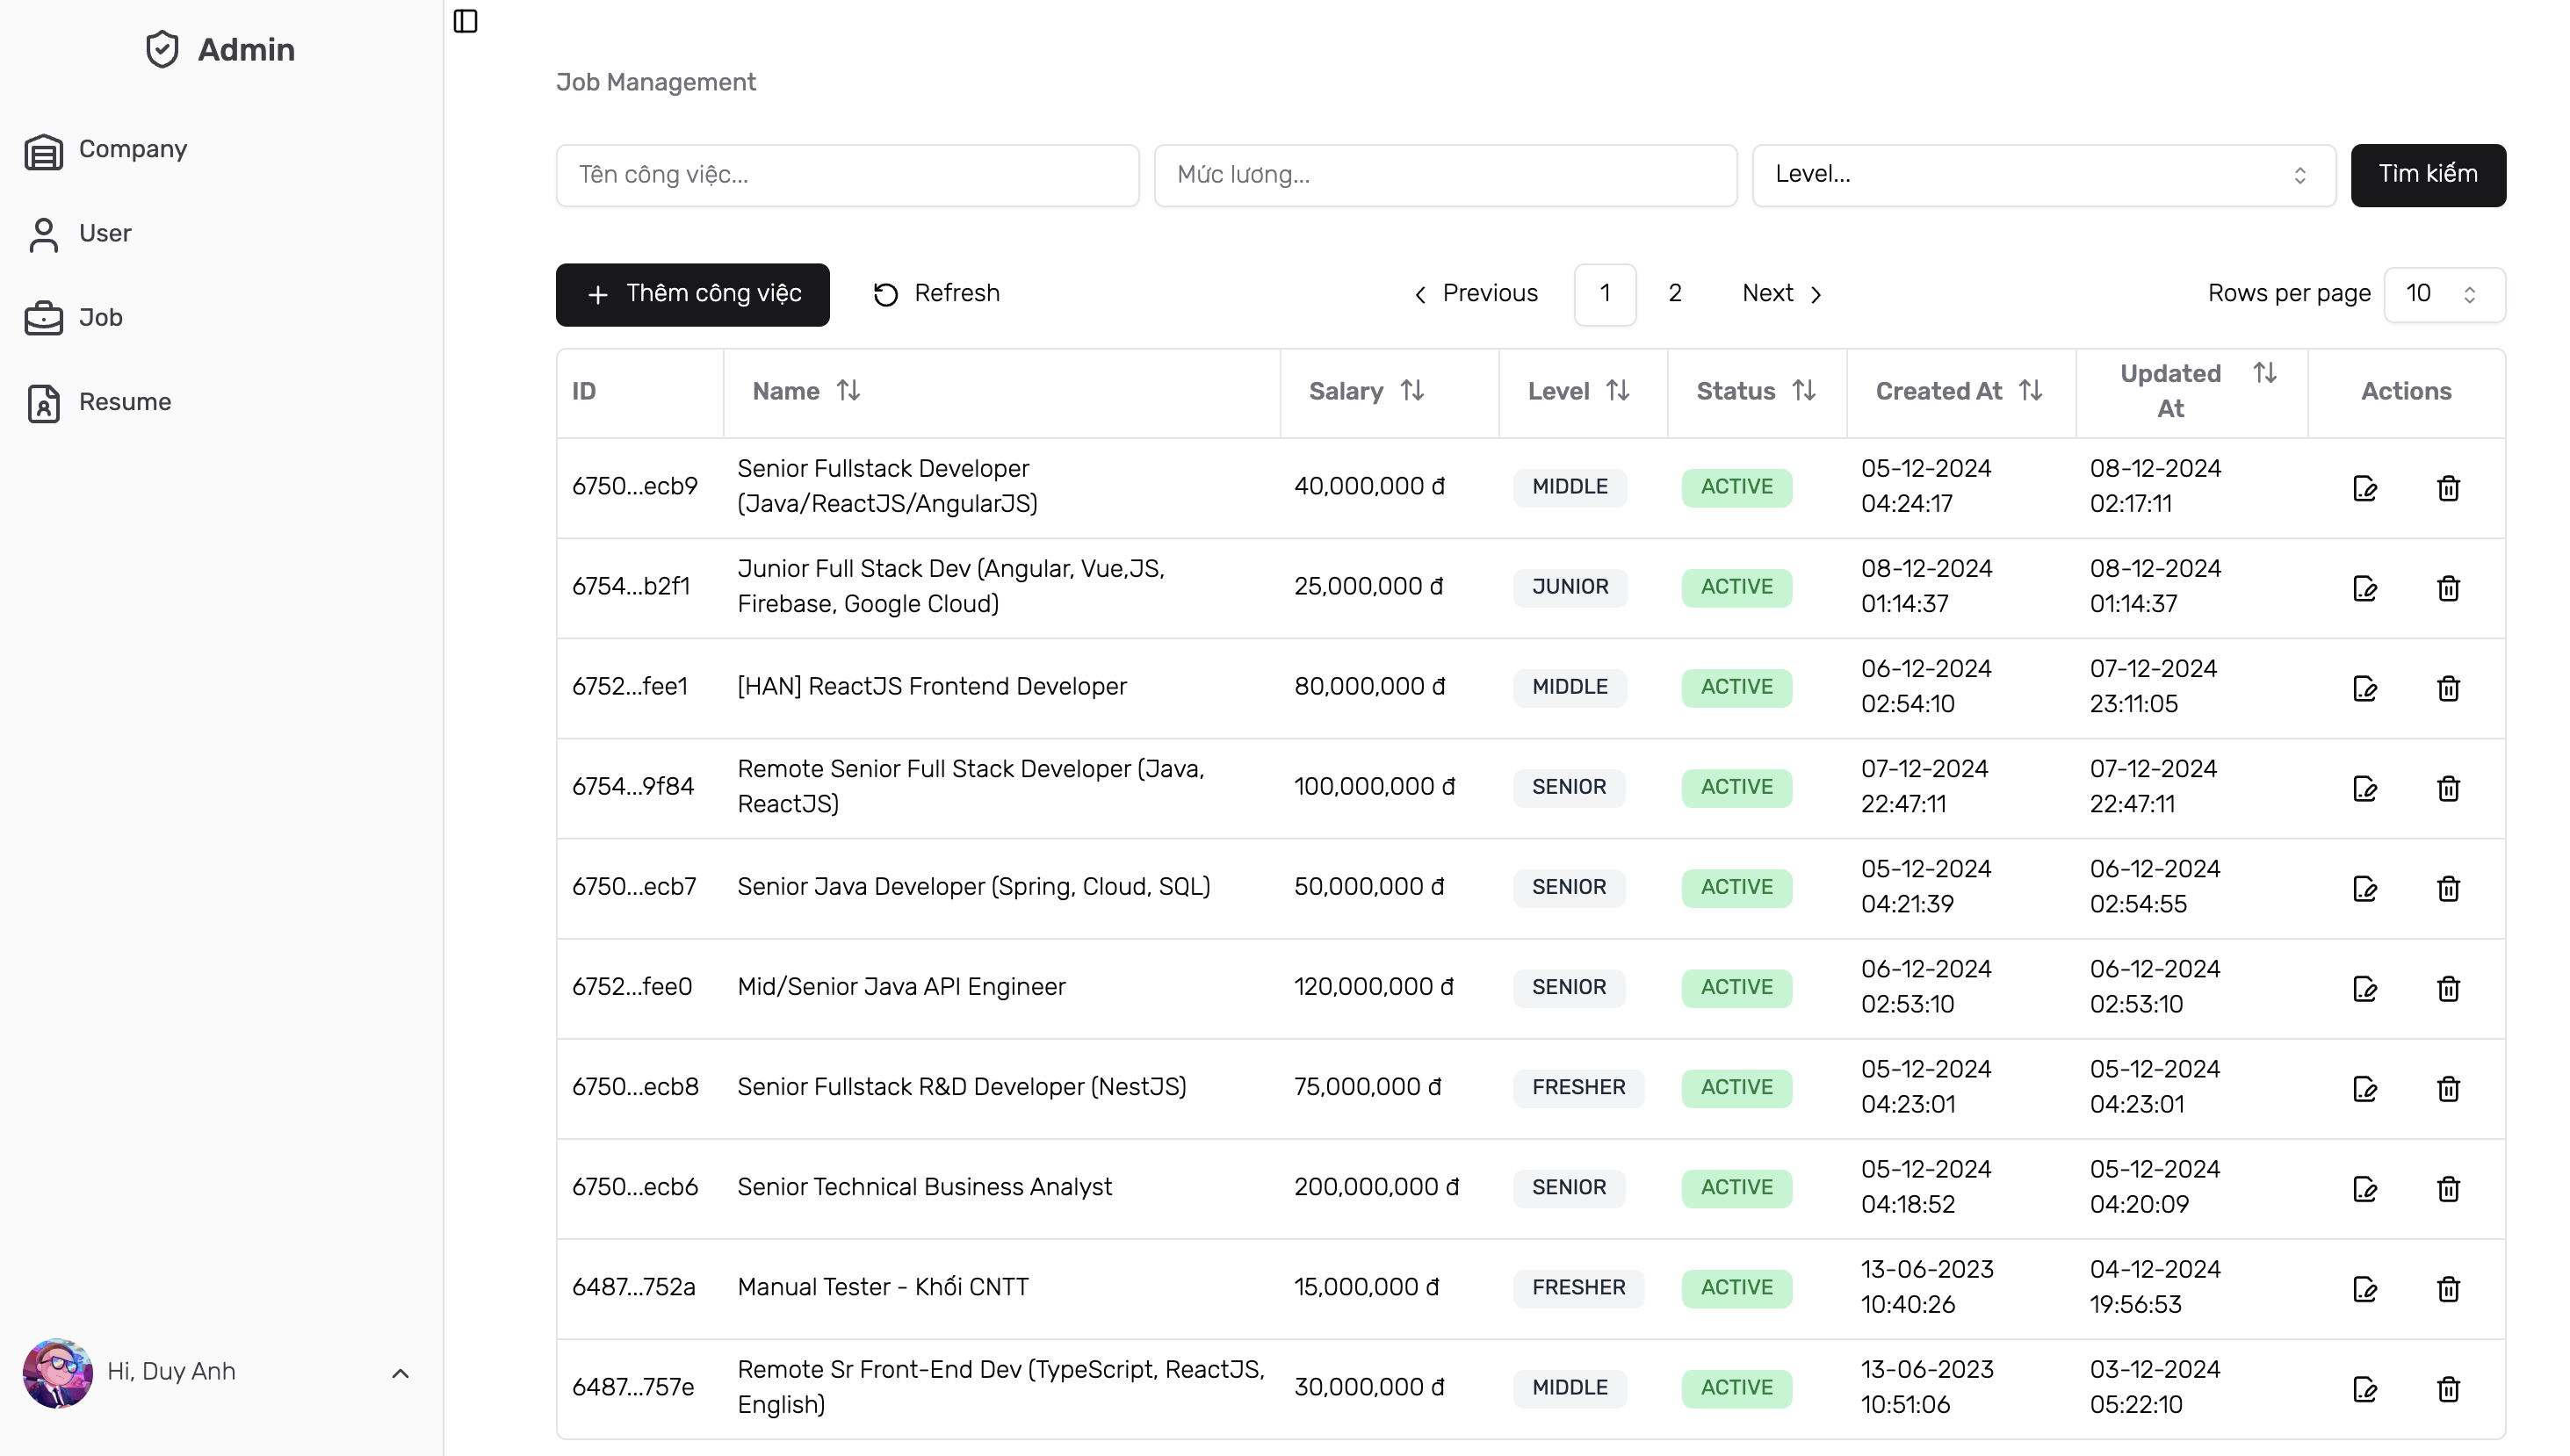
\includegraphics[width=\linewidth]{DBMS-Application/Images/admin-job.png}
    \caption{Trang quản lý công việc - Danh sách các công việc trong hệ thống}
    \label{fig:enter-label}
\end{figure}

Quản trị viên cũng có thể tìm kiếm và lọc ra các công ty theo \textbf{Tên}, \textbf{Mức lương} và \textbf{Level} như sau:

\begin{figure}[H]
    \centering
    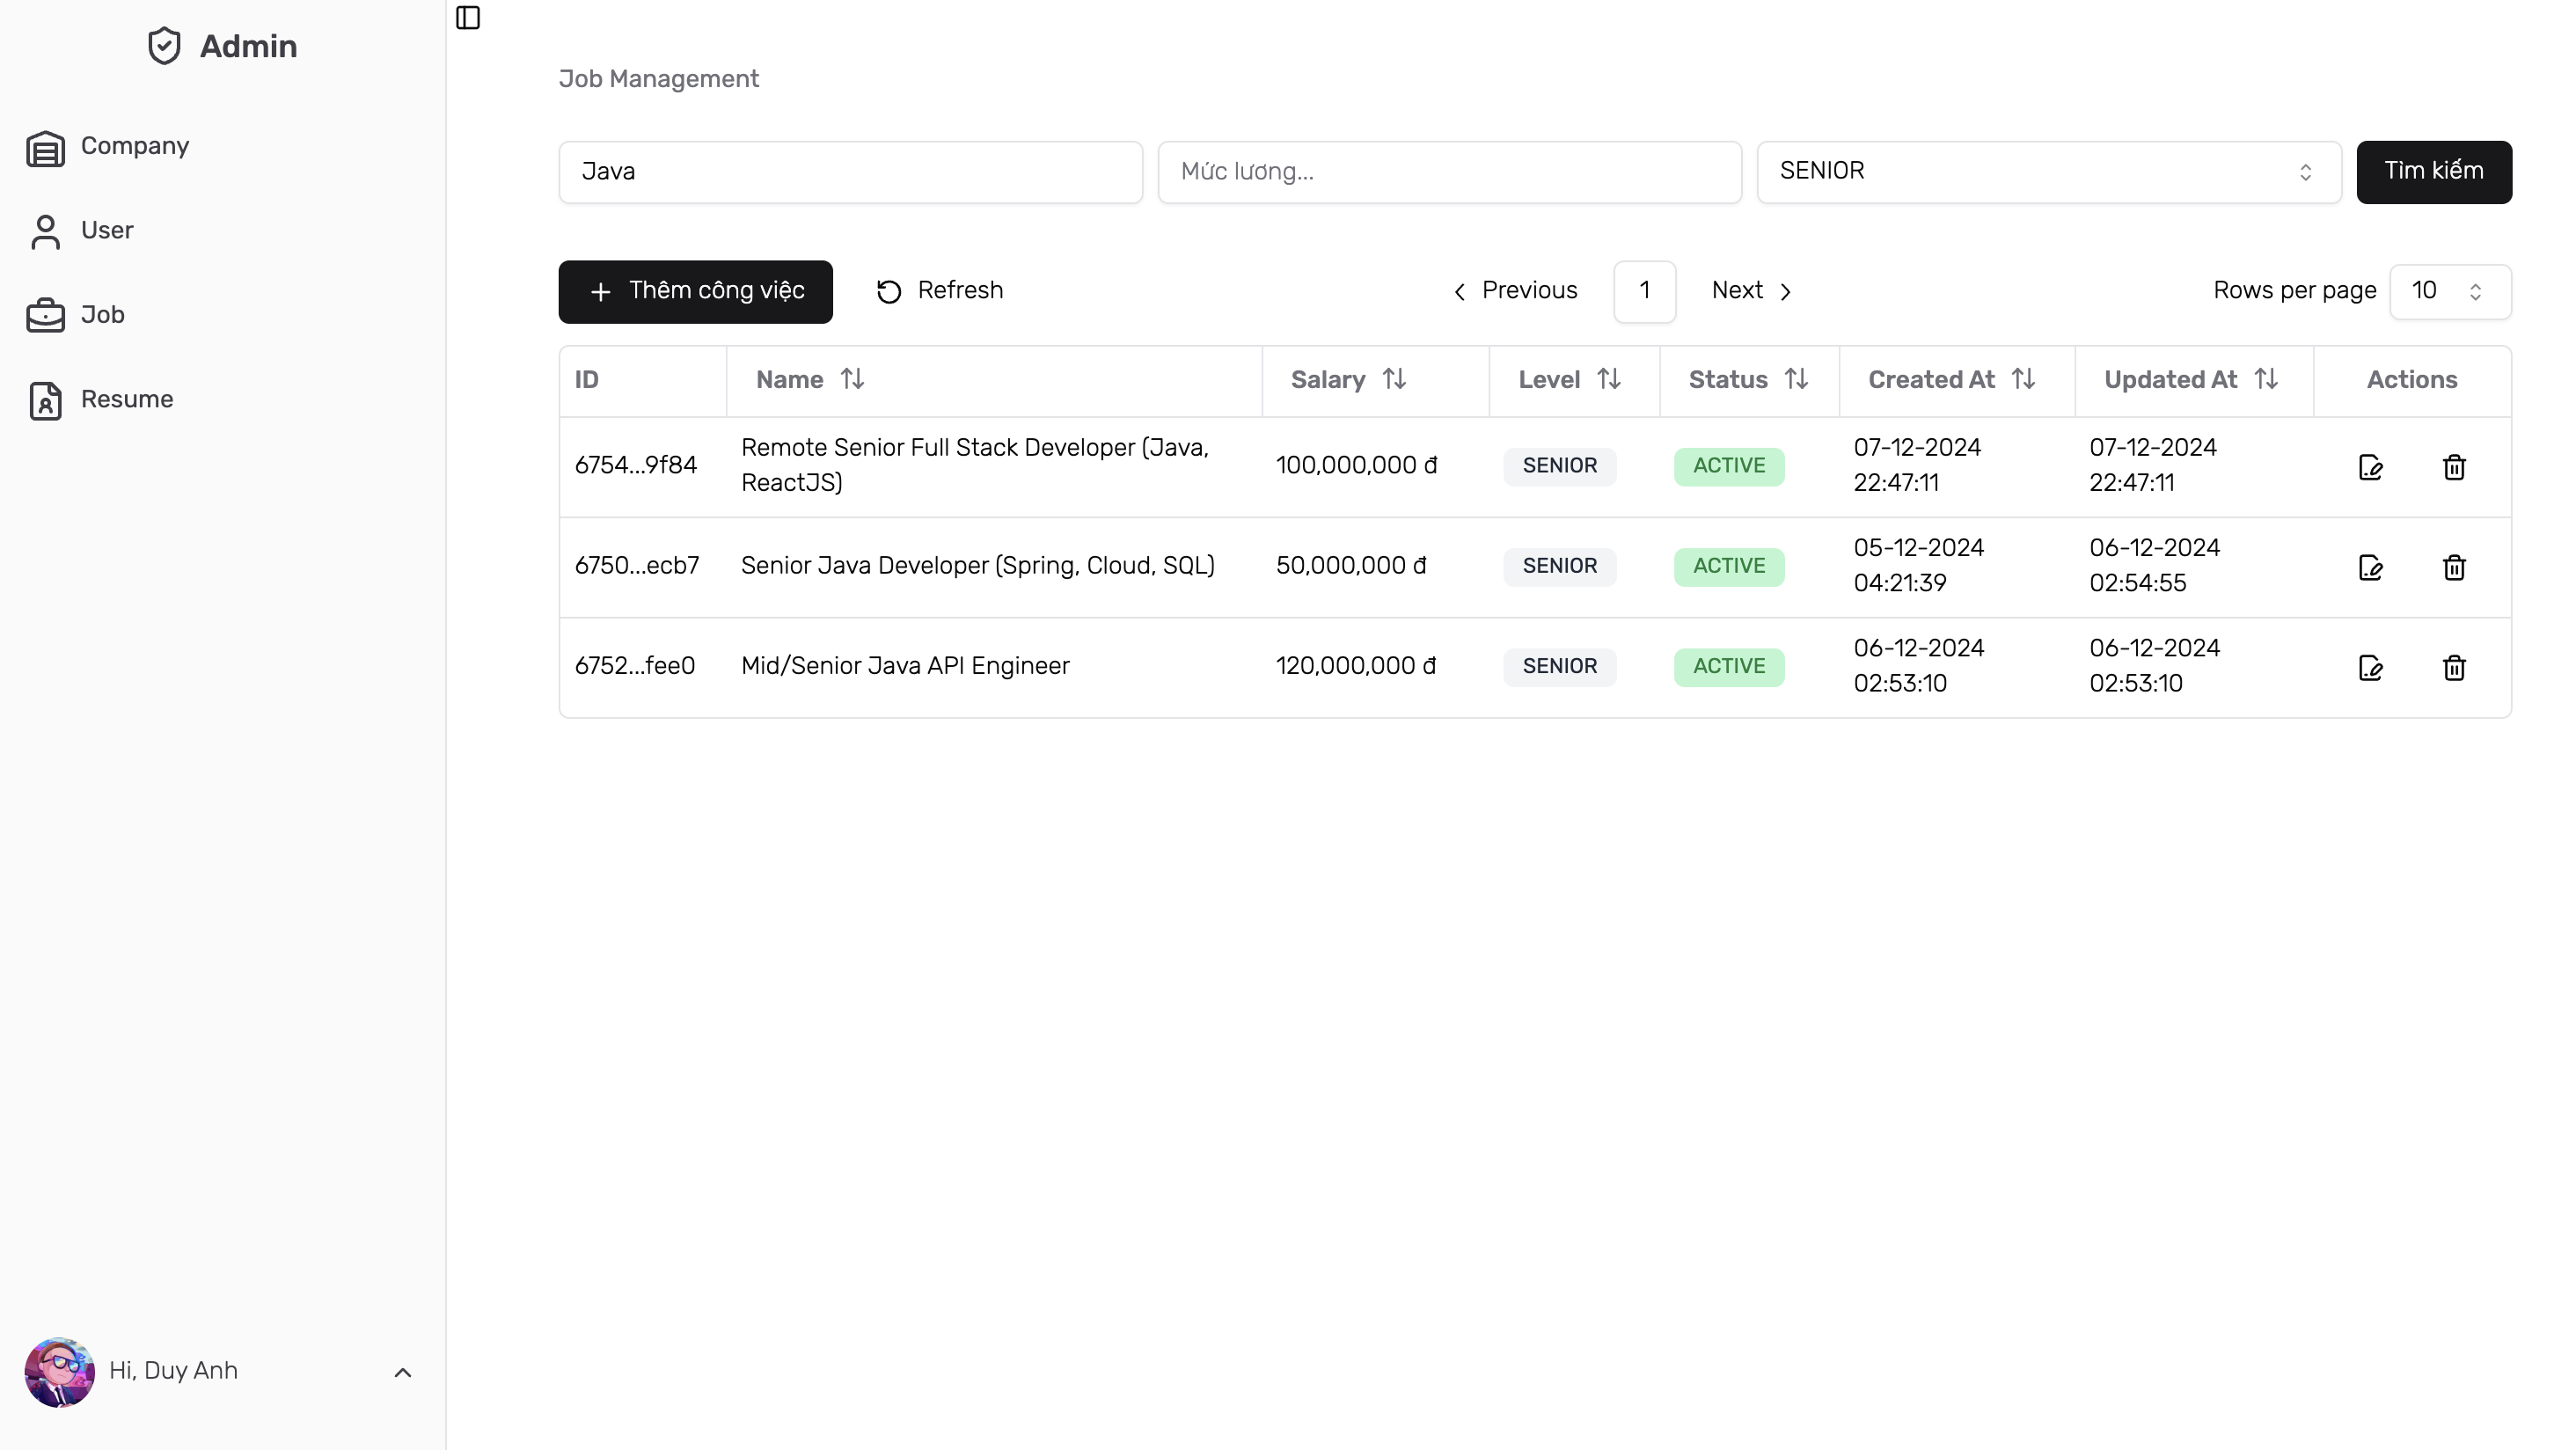
\includegraphics[width=\linewidth]{DBMS-Application/Images/admin-job-filter.png}
    \caption{Trang quản lý công việc - Danh sách công việc lọc theo điều kiện}
    \label{fig:enter-label}
\end{figure}

Truy vấn sử dụng: \textbf{Query with single/composite condition}\\

Bên cạnh đó, quản trị viên cũng có thể thêm công việc mới, bằng cách điền các thông tin cần thiết vào giao diện dưới đây. Sau đó, hệ thống sẽ gửi thông tin này đến cơ sở dữ liệu để thực hiện việc thêm document mới vào collection \textbf{jobs}.

\begin{figure}[H]
    \centering
    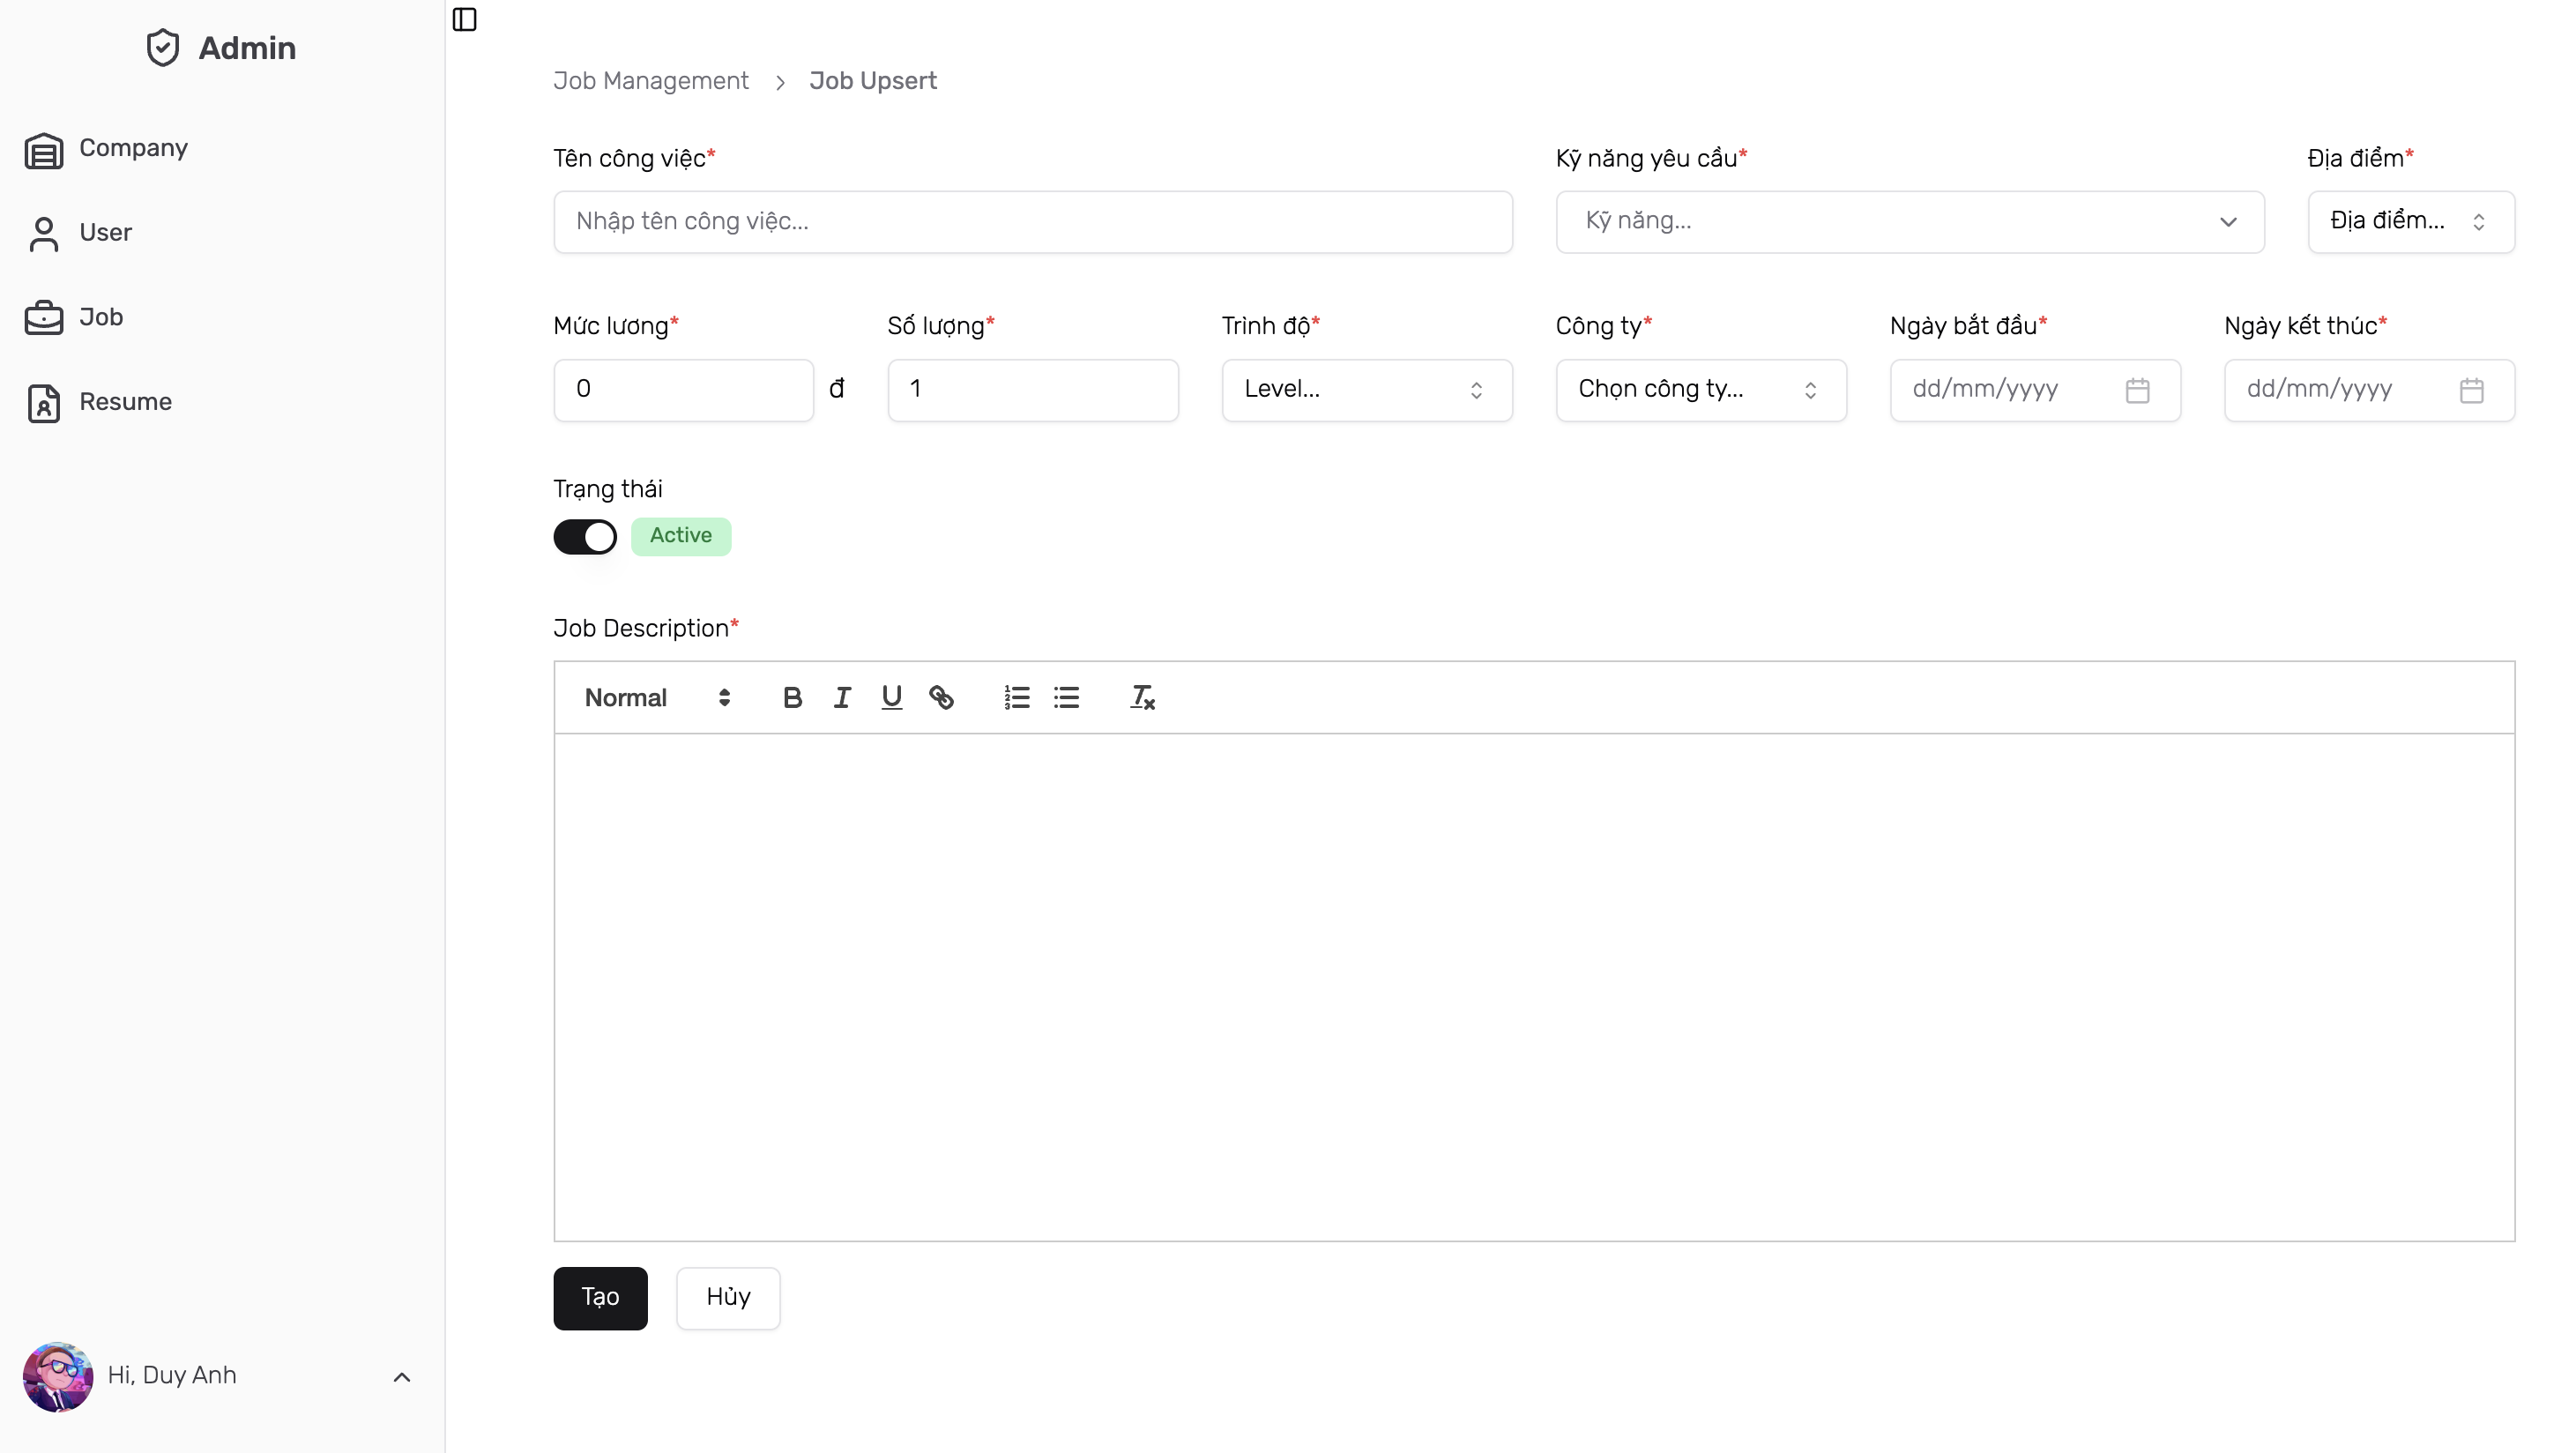
\includegraphics[width=\linewidth]{DBMS-Application/Images/create-job.png}
    \caption{Trang quản lý công việc - Thêm công việc mới}
    \label{fig:enter-label}
\end{figure}

Truy vấn sử dụng: \textbf{Insert}

\begin{lstlisting}
async create(createJobDto: CreateJobDto) {
    const job = {
      ...createJobDto,
      createdAt: new Date(),
      updatedAt: new Date(),
    };

    const result = await this.db.collection('jobs').insertOne(job); // Insert cong viec moi vao collection 'jobs'
    return { _id: result.insertedId, createdAt: job.createdAt };
}
\end{lstlisting}

Quản trị viên cũng có thể chọn một công việc để chỉnh sửa/cập nhật thông tin. Khi đó, dựa vào \texttt{\_id}, hệ thống sẽ truy vấn cơ sở dữ liệu để lấy ra công việc đó (\textbf{query with single condition}) và hiển thị lên giao diện. Lúc này, quản trị viên có thể tiến hành sửa lại các thông tin đó và khi hoàn tất, Front-end sẽ gửi yêu cầu qua API với phương thức HTTP \textbf{PATCH} để hệ thống tiến hành cập nhật lại thông tin cho công việc đó trong cơ sở dữ liệu.

\begin{figure}[H]
    \centering
    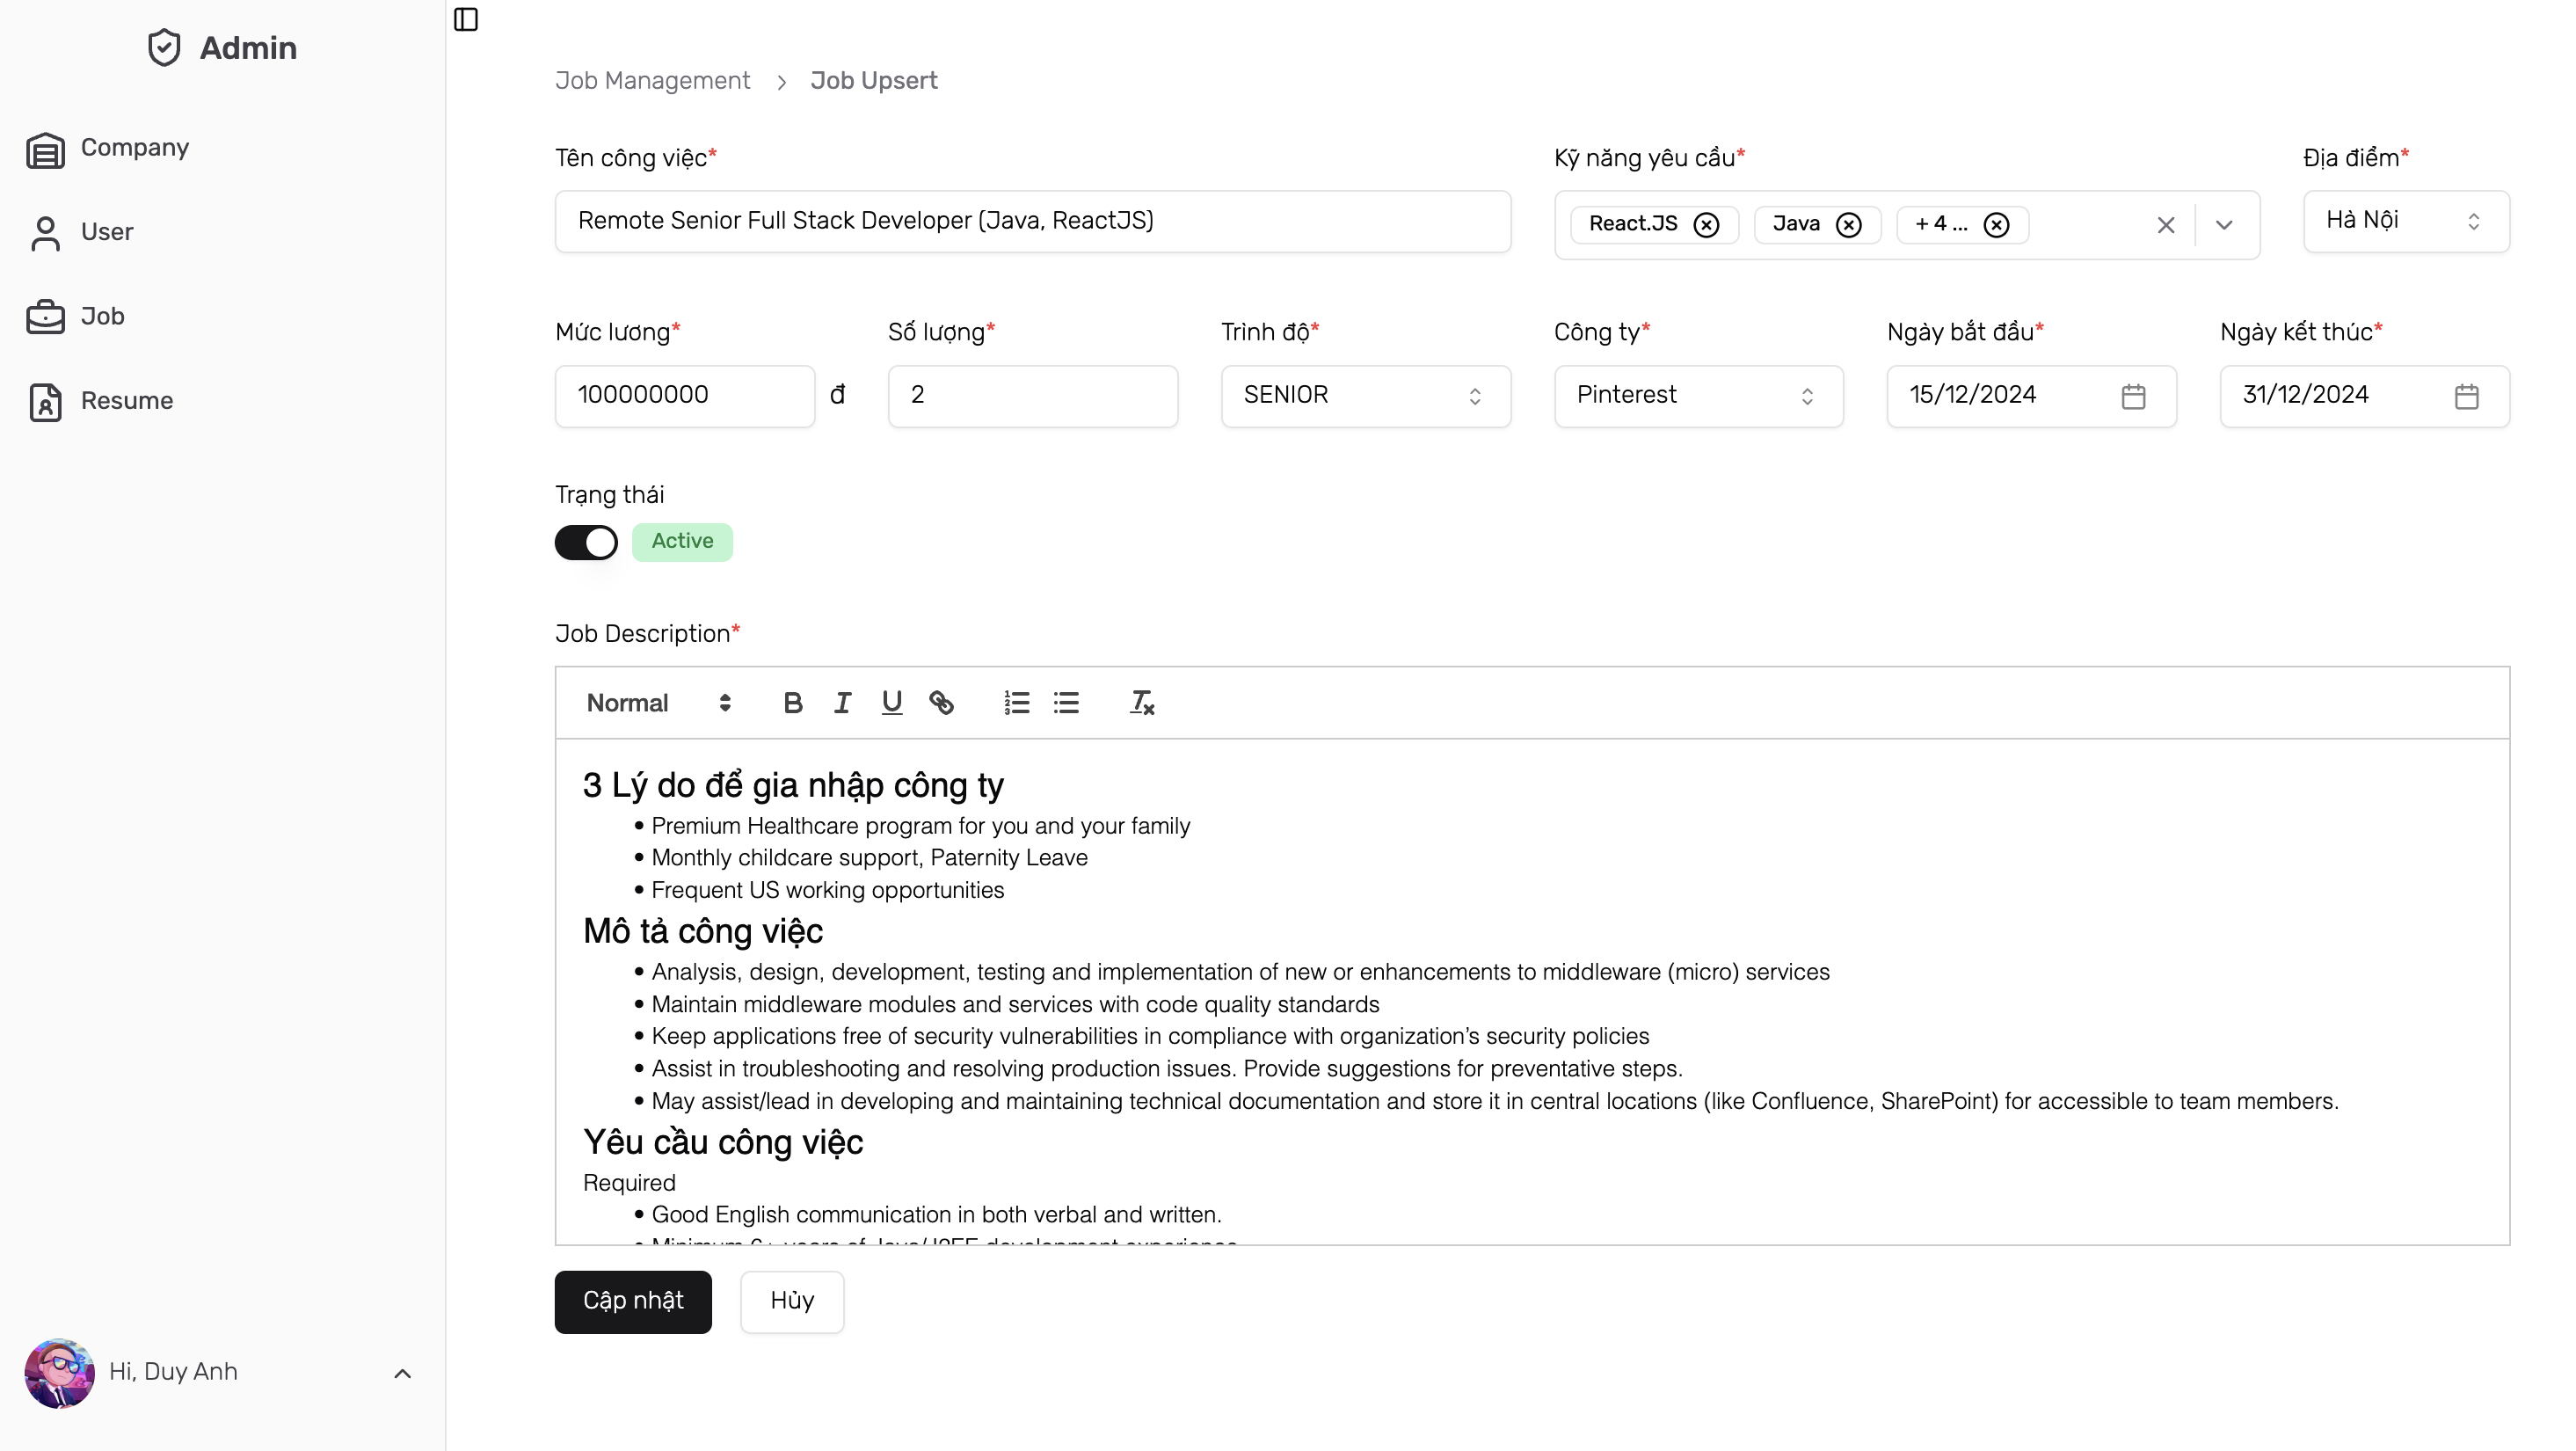
\includegraphics[width=\linewidth]{DBMS-Application/Images/update-job.png}
    \caption{Trang quản lý công việc - Cập nhật thông tin cho một công việc cụ thể}
    \label{fig:enter-label}
\end{figure}

Truy vấn sử dụng: \textbf{Update}

\begin{lstlisting}
const result = await this.db.collection('jobs').updateOne(
  { _id: new ObjectId(id) },
  {
    $set: {
      ...updateJobDto,
      updatedAt: new Date(),
    },
  },
);
\end{lstlisting}

Cuối cùng, quản trị viên có thể chọn một công việc để xoá khỏi hệ thống. Khi đó, một popup sẽ hiện lên để xác nhận với quản trị viên về việc xoá công ty đã chọn ra khỏi cơ sở dữ liệu

\begin{figure}[H]
    \centering
    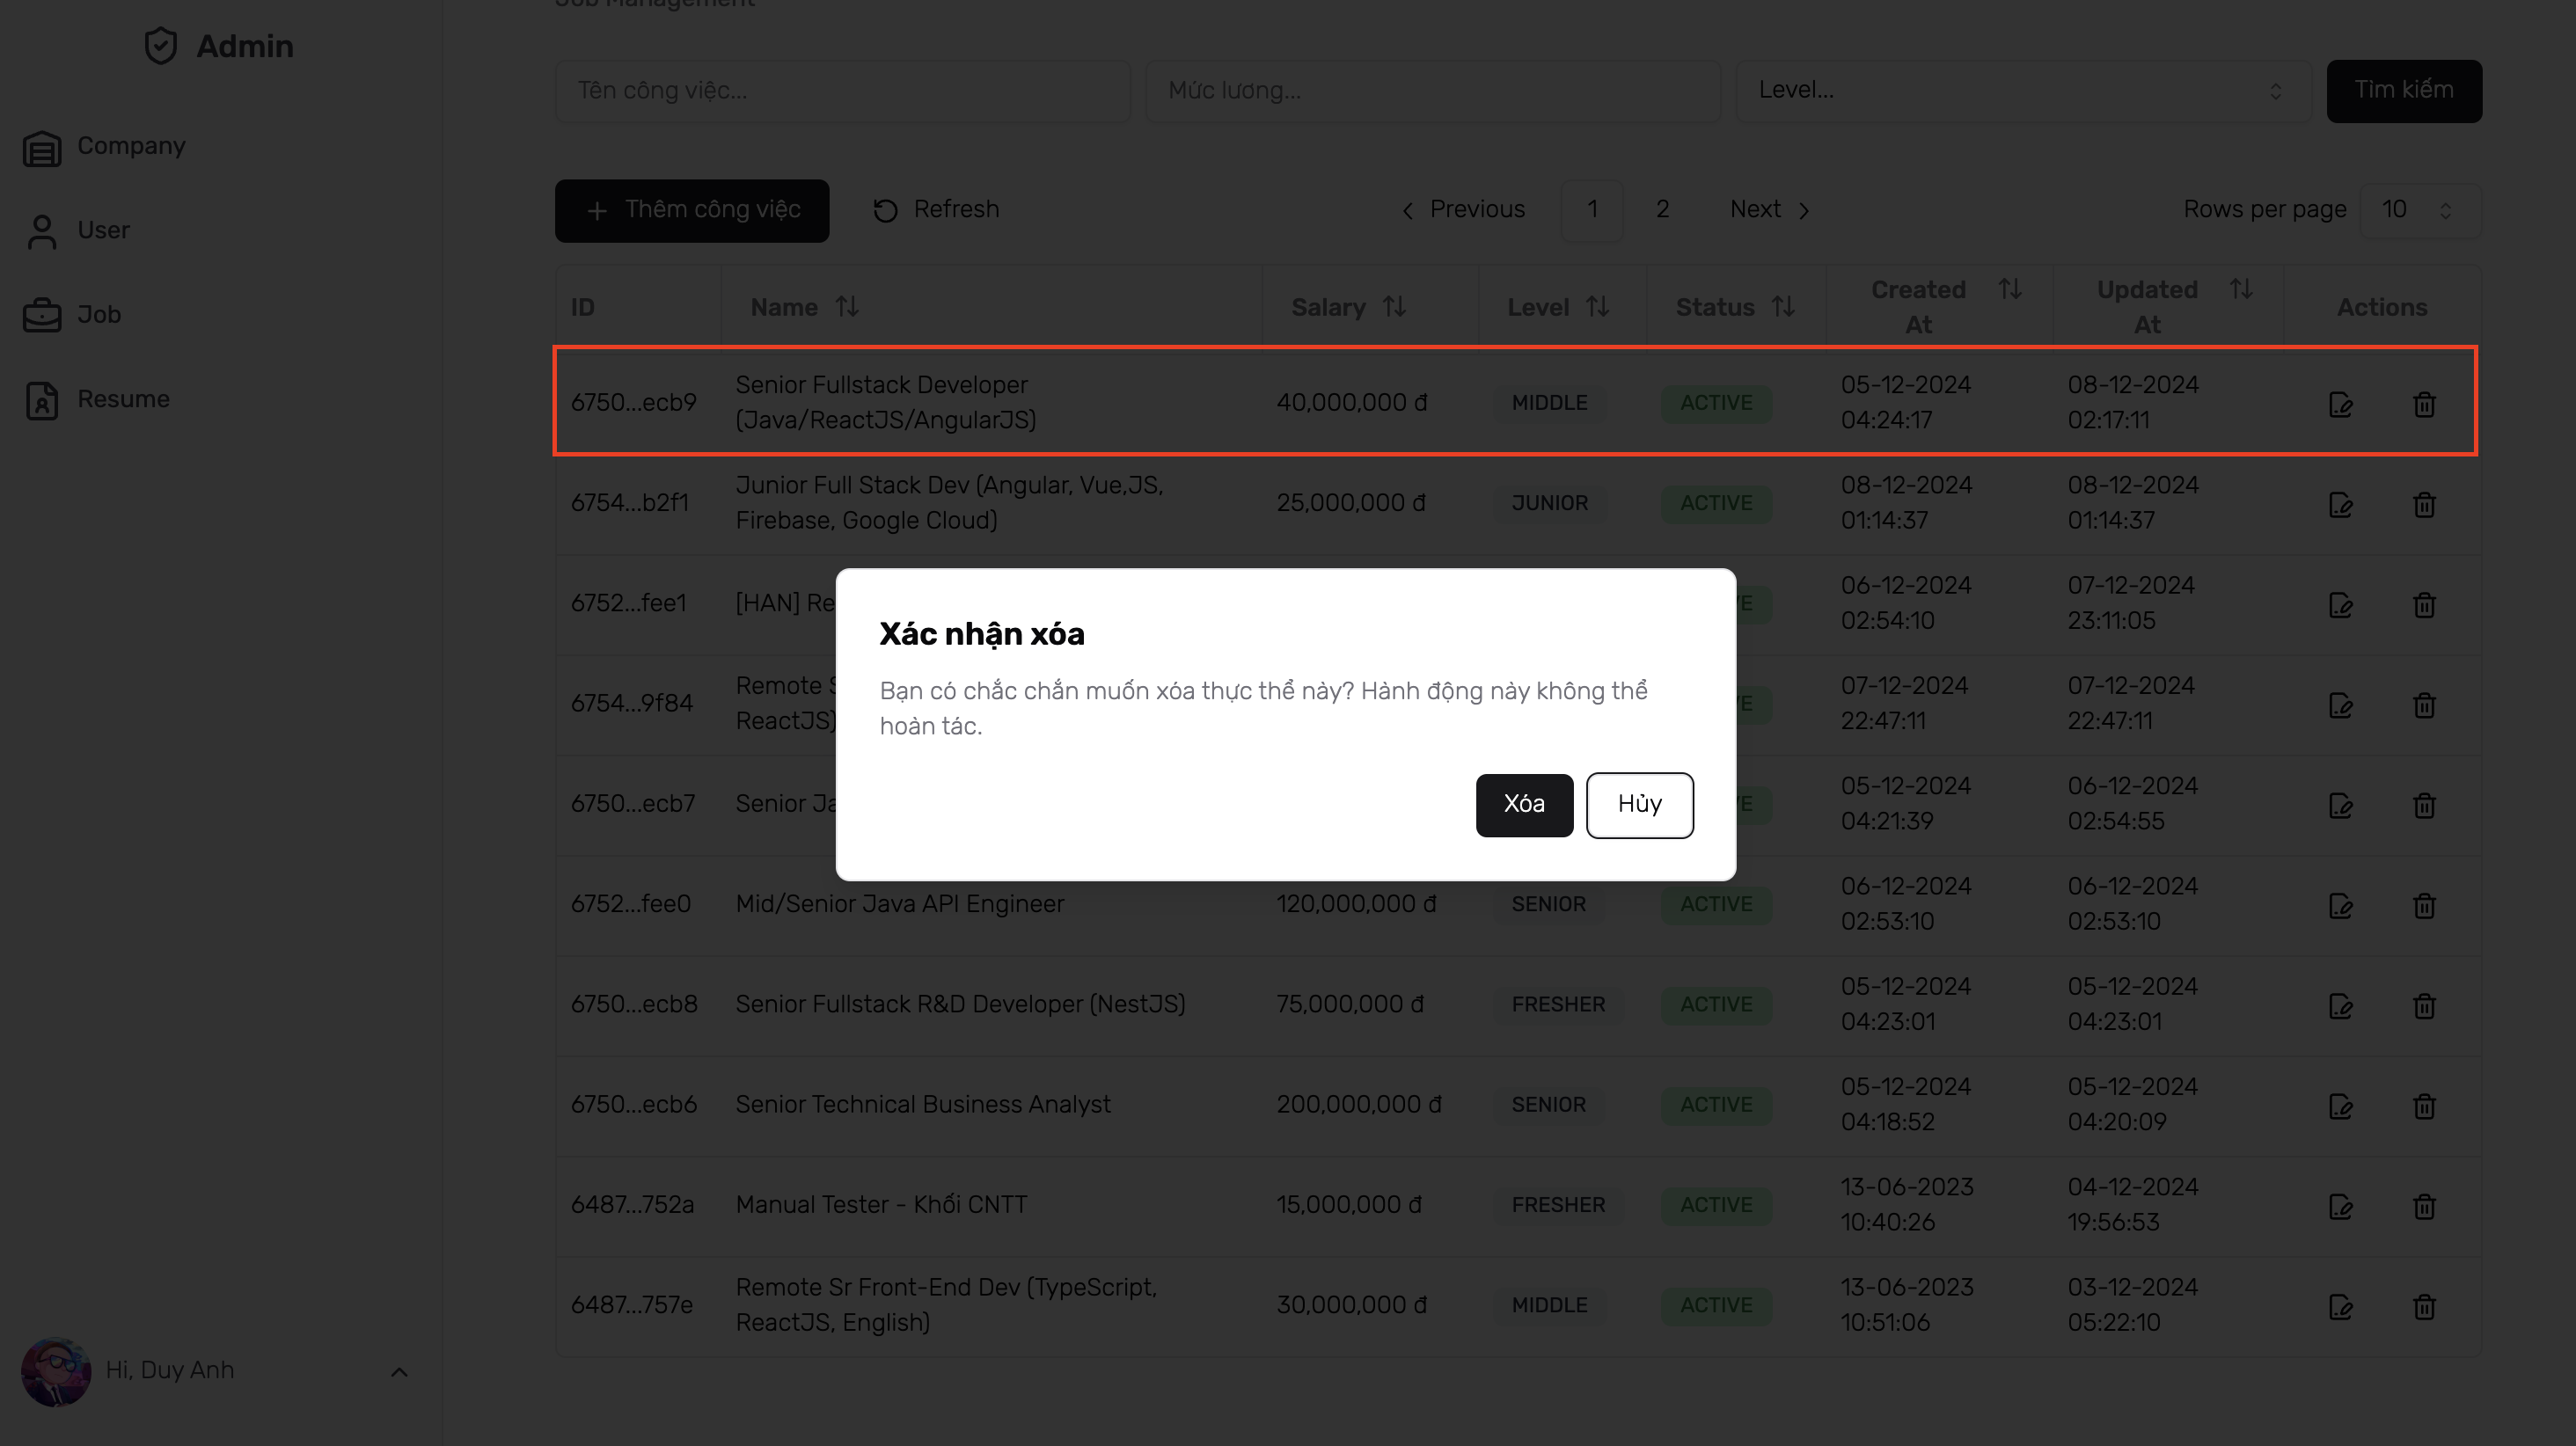
\includegraphics[width=\linewidth]{DBMS-Application/Images/delete-job.png}
    \caption{Trang quản lý công việc - Xác nhận xoá công việc chỉ định khỏi hệ thống}
    \label{fig:enter-label}
\end{figure}

Khi quản trị viên xác nhận, Back-end gửi truy vấn đến cơ sở dữ liệu để tìm theo \texttt{\_id} và xoá công việc đó ra khỏi cơ sở dữ liệu. Khi đó, giao diện người dùng sẽ được cập nhật lại.\\

\begin{figure}[H]
    \centering
    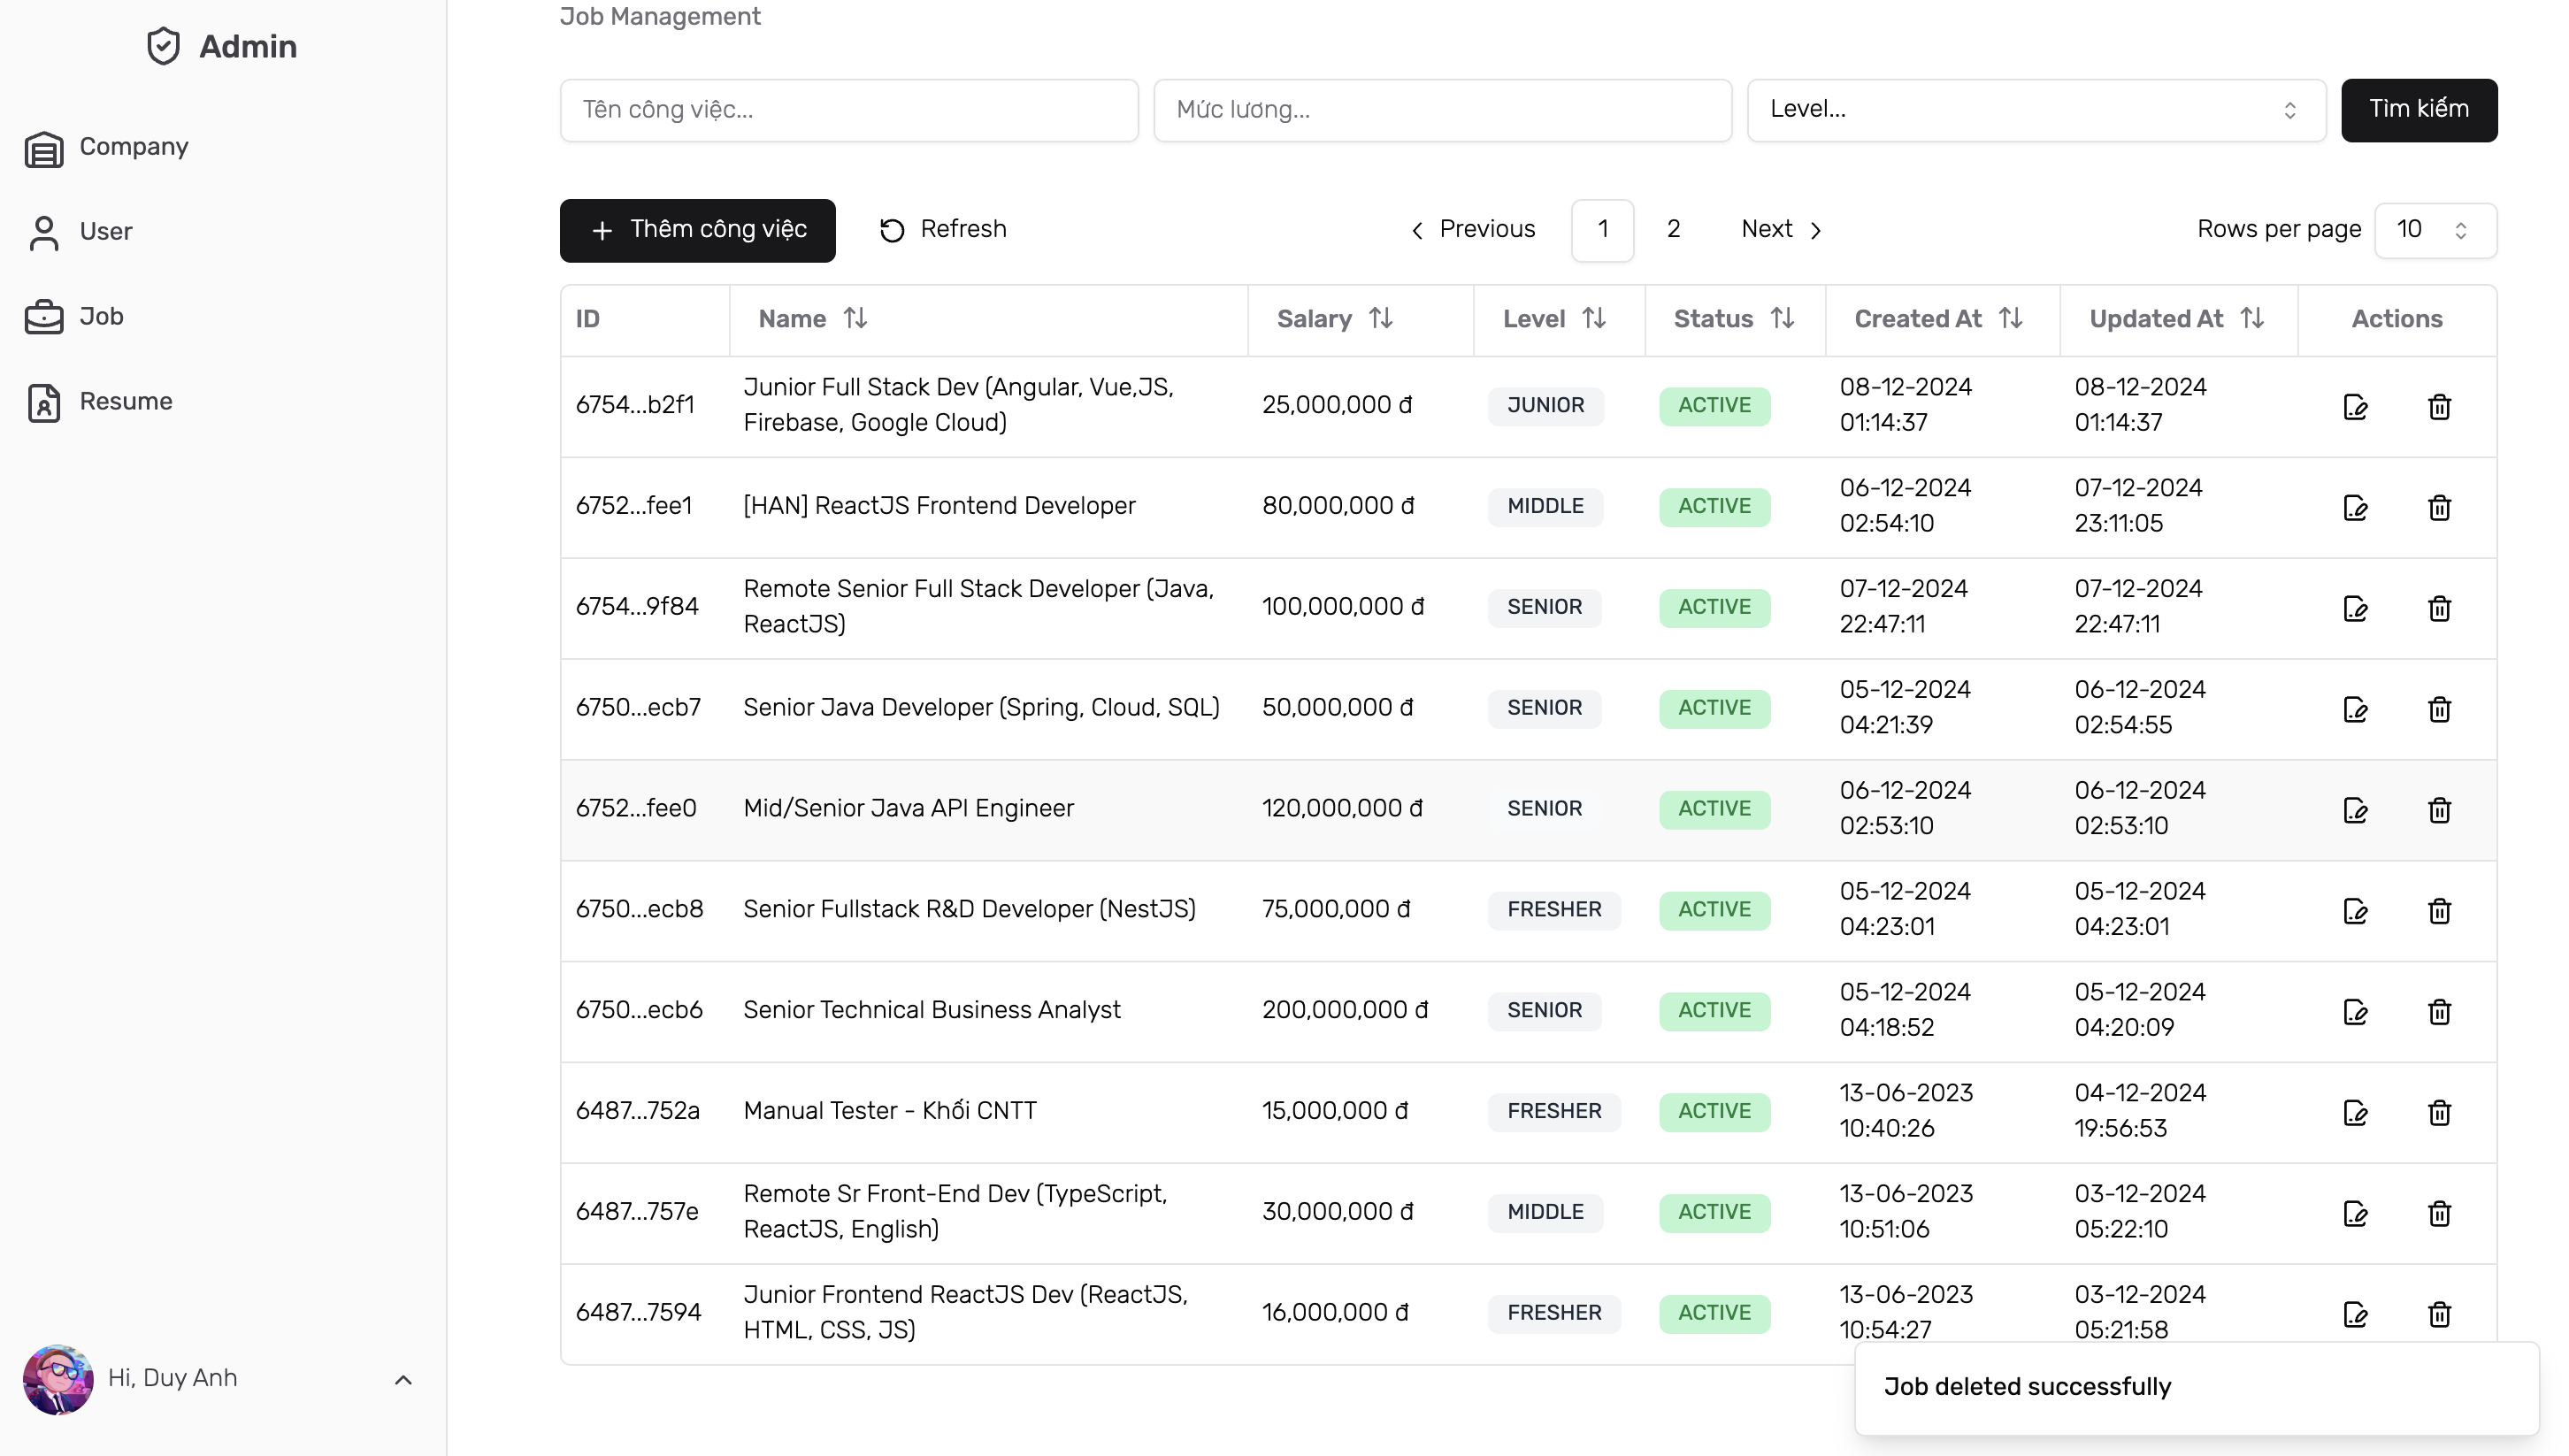
\includegraphics[width=\linewidth]{DBMS-Application/Images/delete-job-successfully.png}
    \caption{Trang quản lý công việc - Xoá thành công công việc đã chọn}
    \label{fig:enter-label}
\end{figure}

Truy vấn sử dụng: \textbf{Delete}

\begin{lstlisting}
const result = await this.db
      .collection('jobs')
      .deleteOne({ _id: new ObjectId(id) });
\end{lstlisting}

% \subsubsection{Giao diện Admin - Quản lý công ty}

Tương tự trang quản lý công việc, trang quản lý công ty cũng sử dụng các loại truy vấn sau để hỗ trợ cho các thao tác CRUD:
\begin{itemize}
    \item \textbf{Query with single/composite condition}: Để fetch lên dữ liệu toàn bộ công ty trong hệ thống theo cơ chế phân trang và một số điều kiện như \textbf{Tên công ty}, \textbf{Địa chỉ}
    \begin{figure}[H]
        \centering
        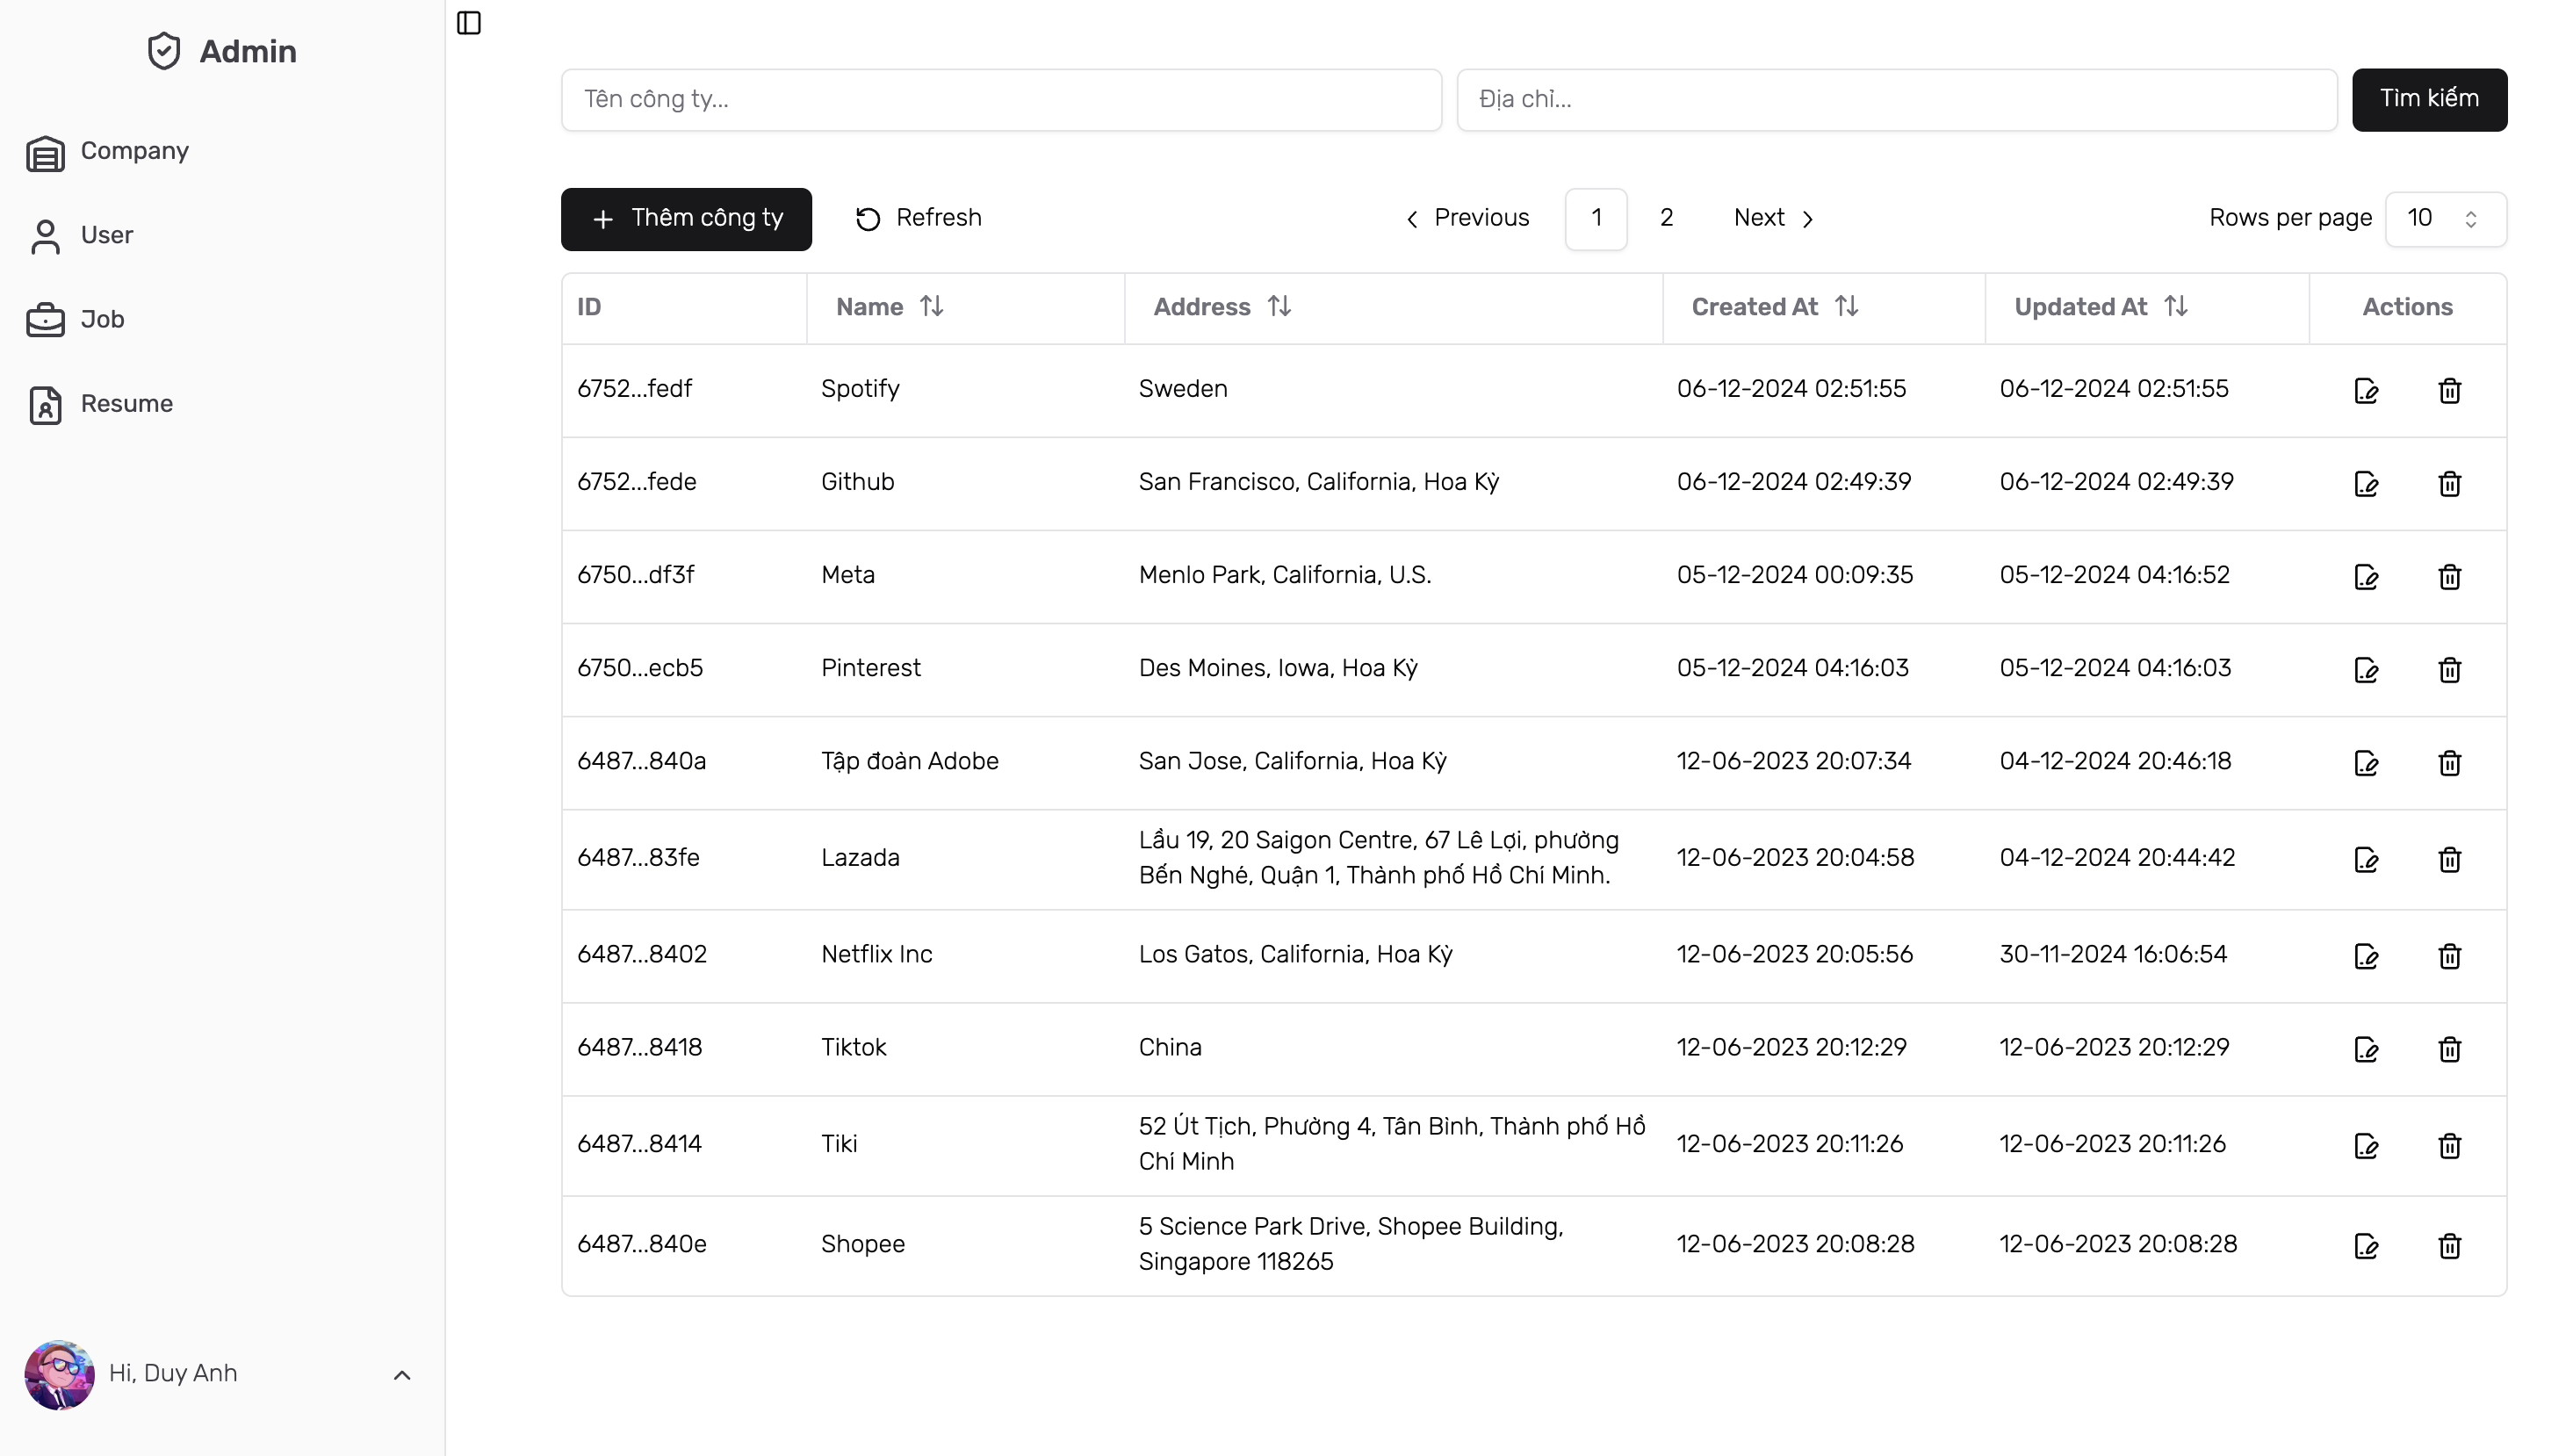
\includegraphics[width=\linewidth]{DBMS-Application/Images/admin-company.png}
        \caption{Trang quản lý công ty - Danh sách các công ty trong hệ thống}
        \label{fig:enter-label}
    \end{figure}

    \begin{figure}[H]
        \centering
        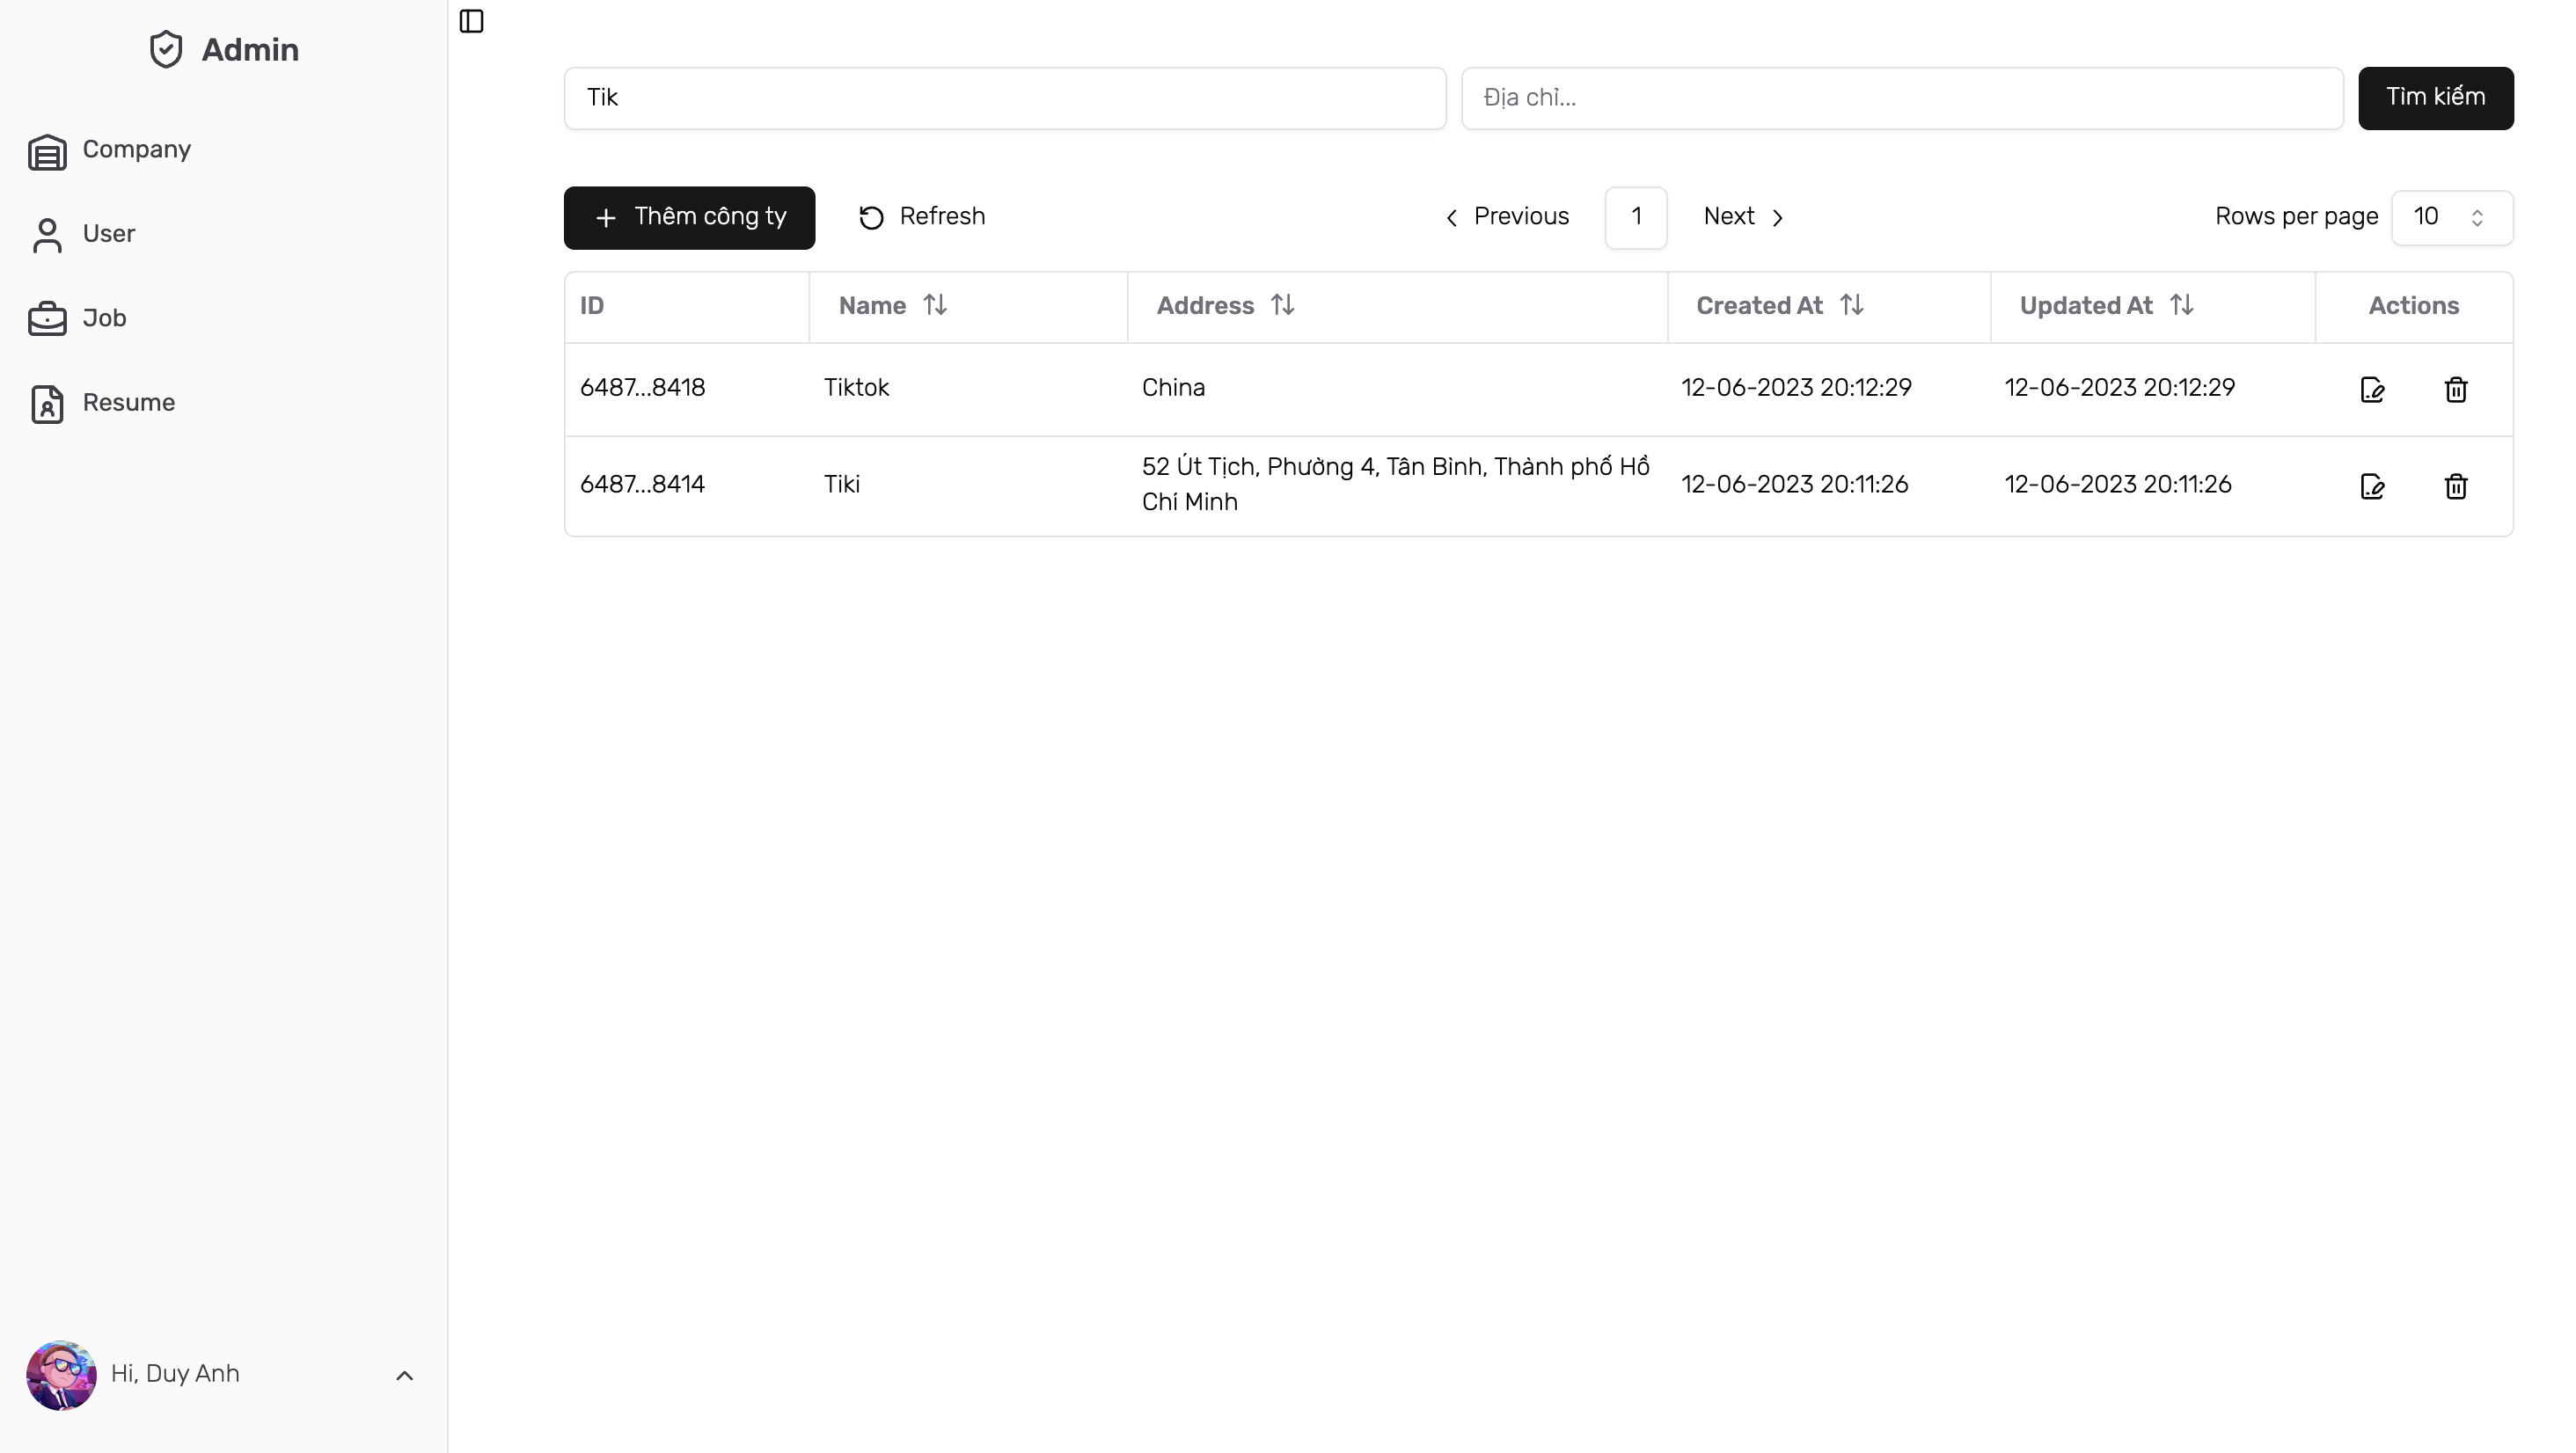
\includegraphics[width=\linewidth]{DBMS-Application/Images/admin-company-filter.png}
        \caption{Trang quản lý công ty - Danh sách công ty lọc theo điều kiện}
        \label{fig:enter-label}
    \end{figure}
    
    \item \textbf{Insert}: Thêm mới một công ty
    \begin{figure}[H]
        \centering
        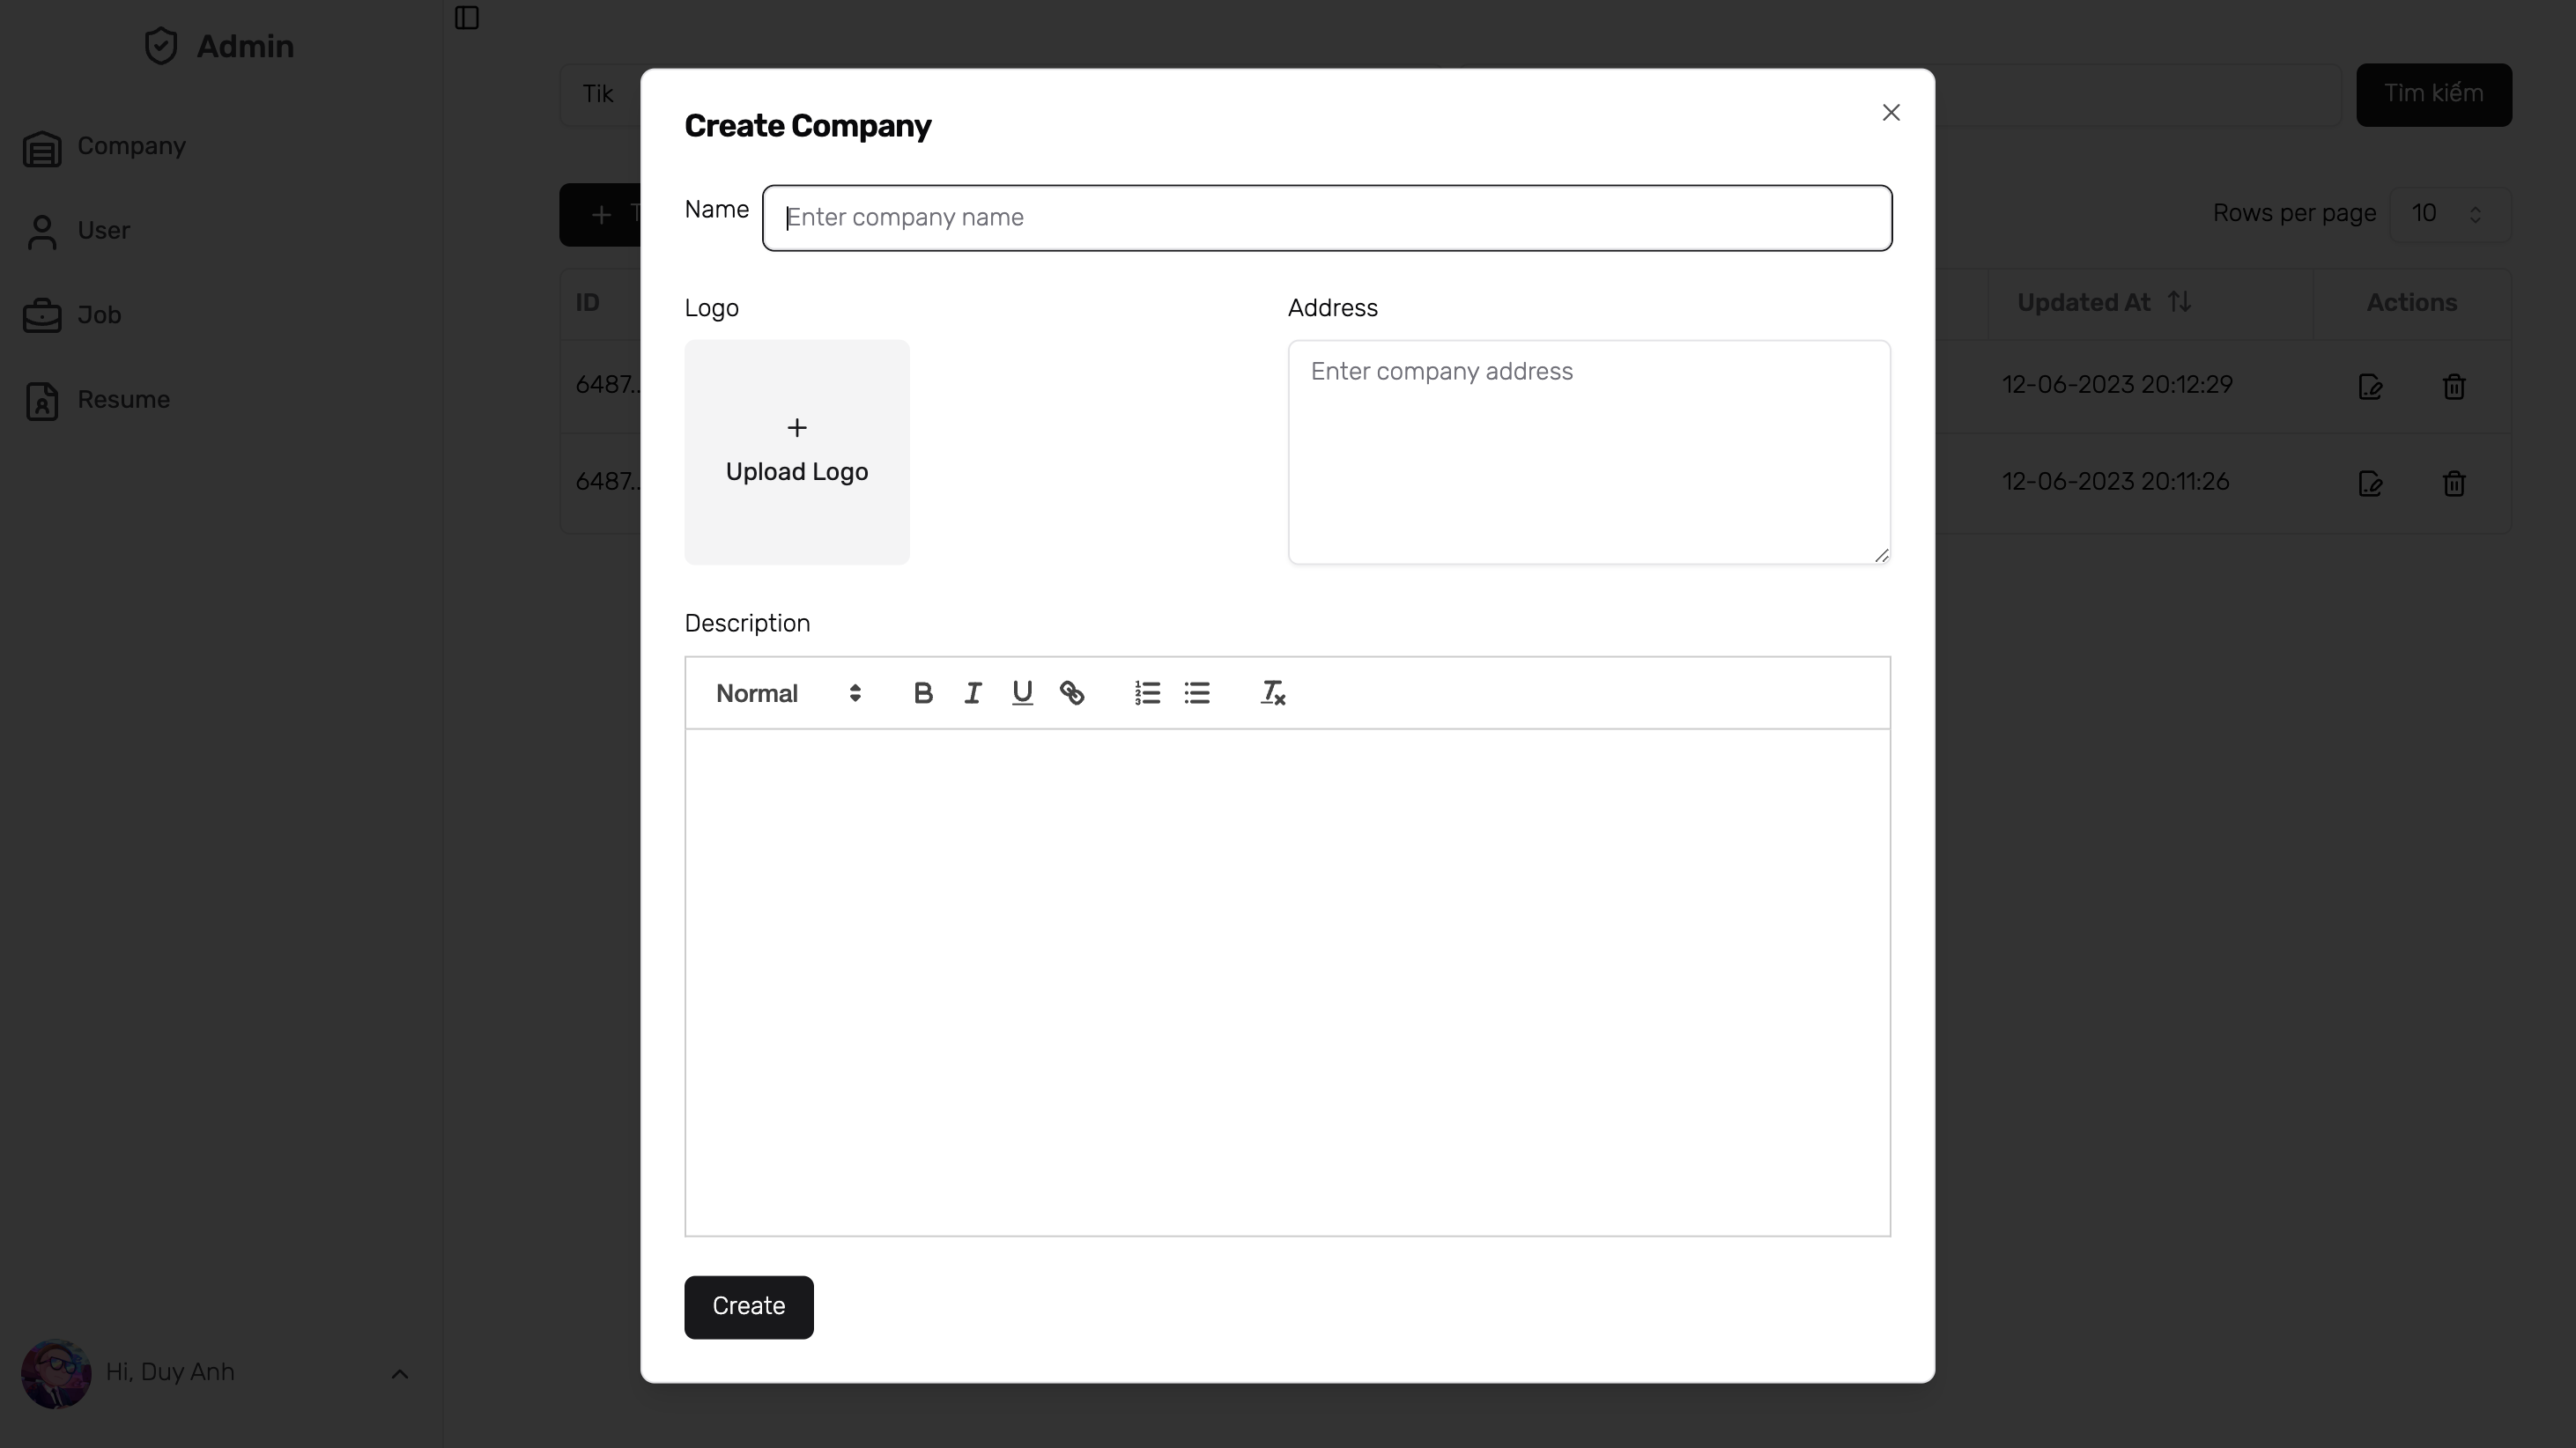
\includegraphics[width=\linewidth]{DBMS-Application/Images/create-company.png}
        \caption{Trang quản lý công ty - Thêm mới công ty}
        \label{fig:enter-label}
    \end{figure}

    \item \textbf{Update}: Cập nhật/chỉnh sửa thông tin công ty cụ thể
    \begin{figure}[H]
        \centering
        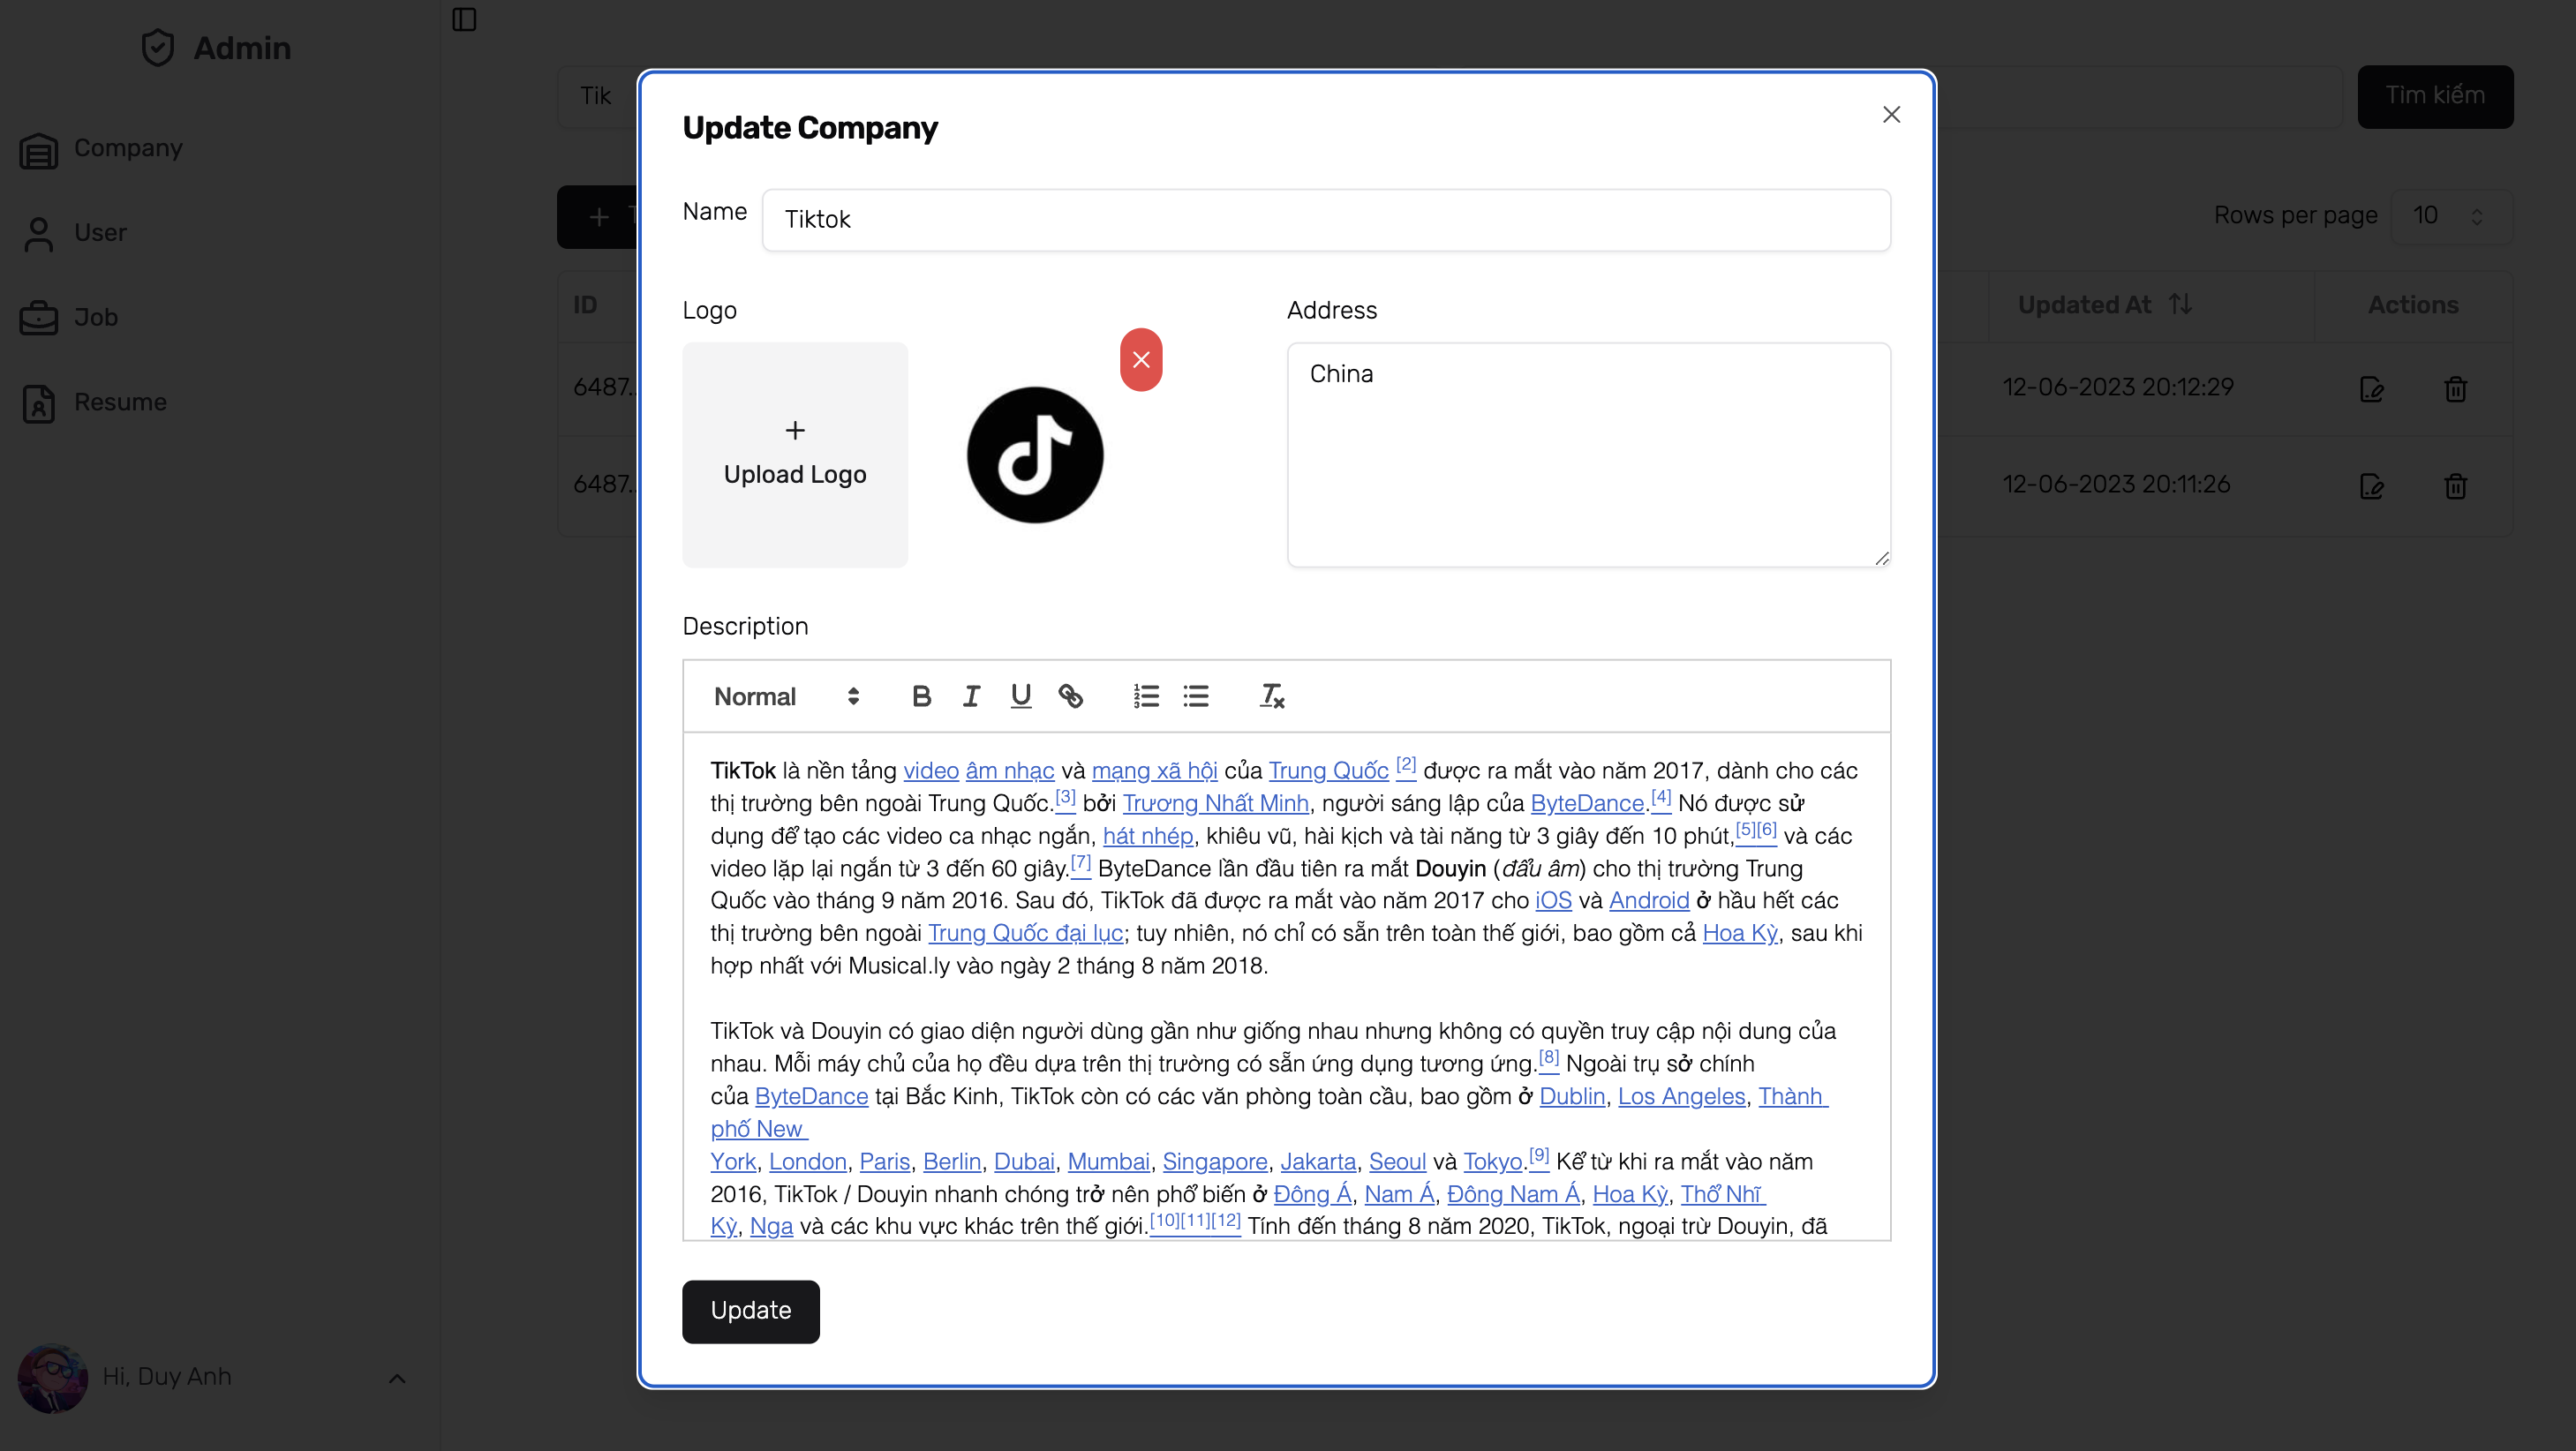
\includegraphics[width=\linewidth]{DBMS-Application/Images/update-company.png}
        \caption{Trang quản lý công ty - Cập nhật thông tin công ty}
        \label{fig:enter-label}
    \end{figure}

    \item \textbf{Delete}: Xoá công ty cụ thể
    \begin{figure}[H]
        \centering
        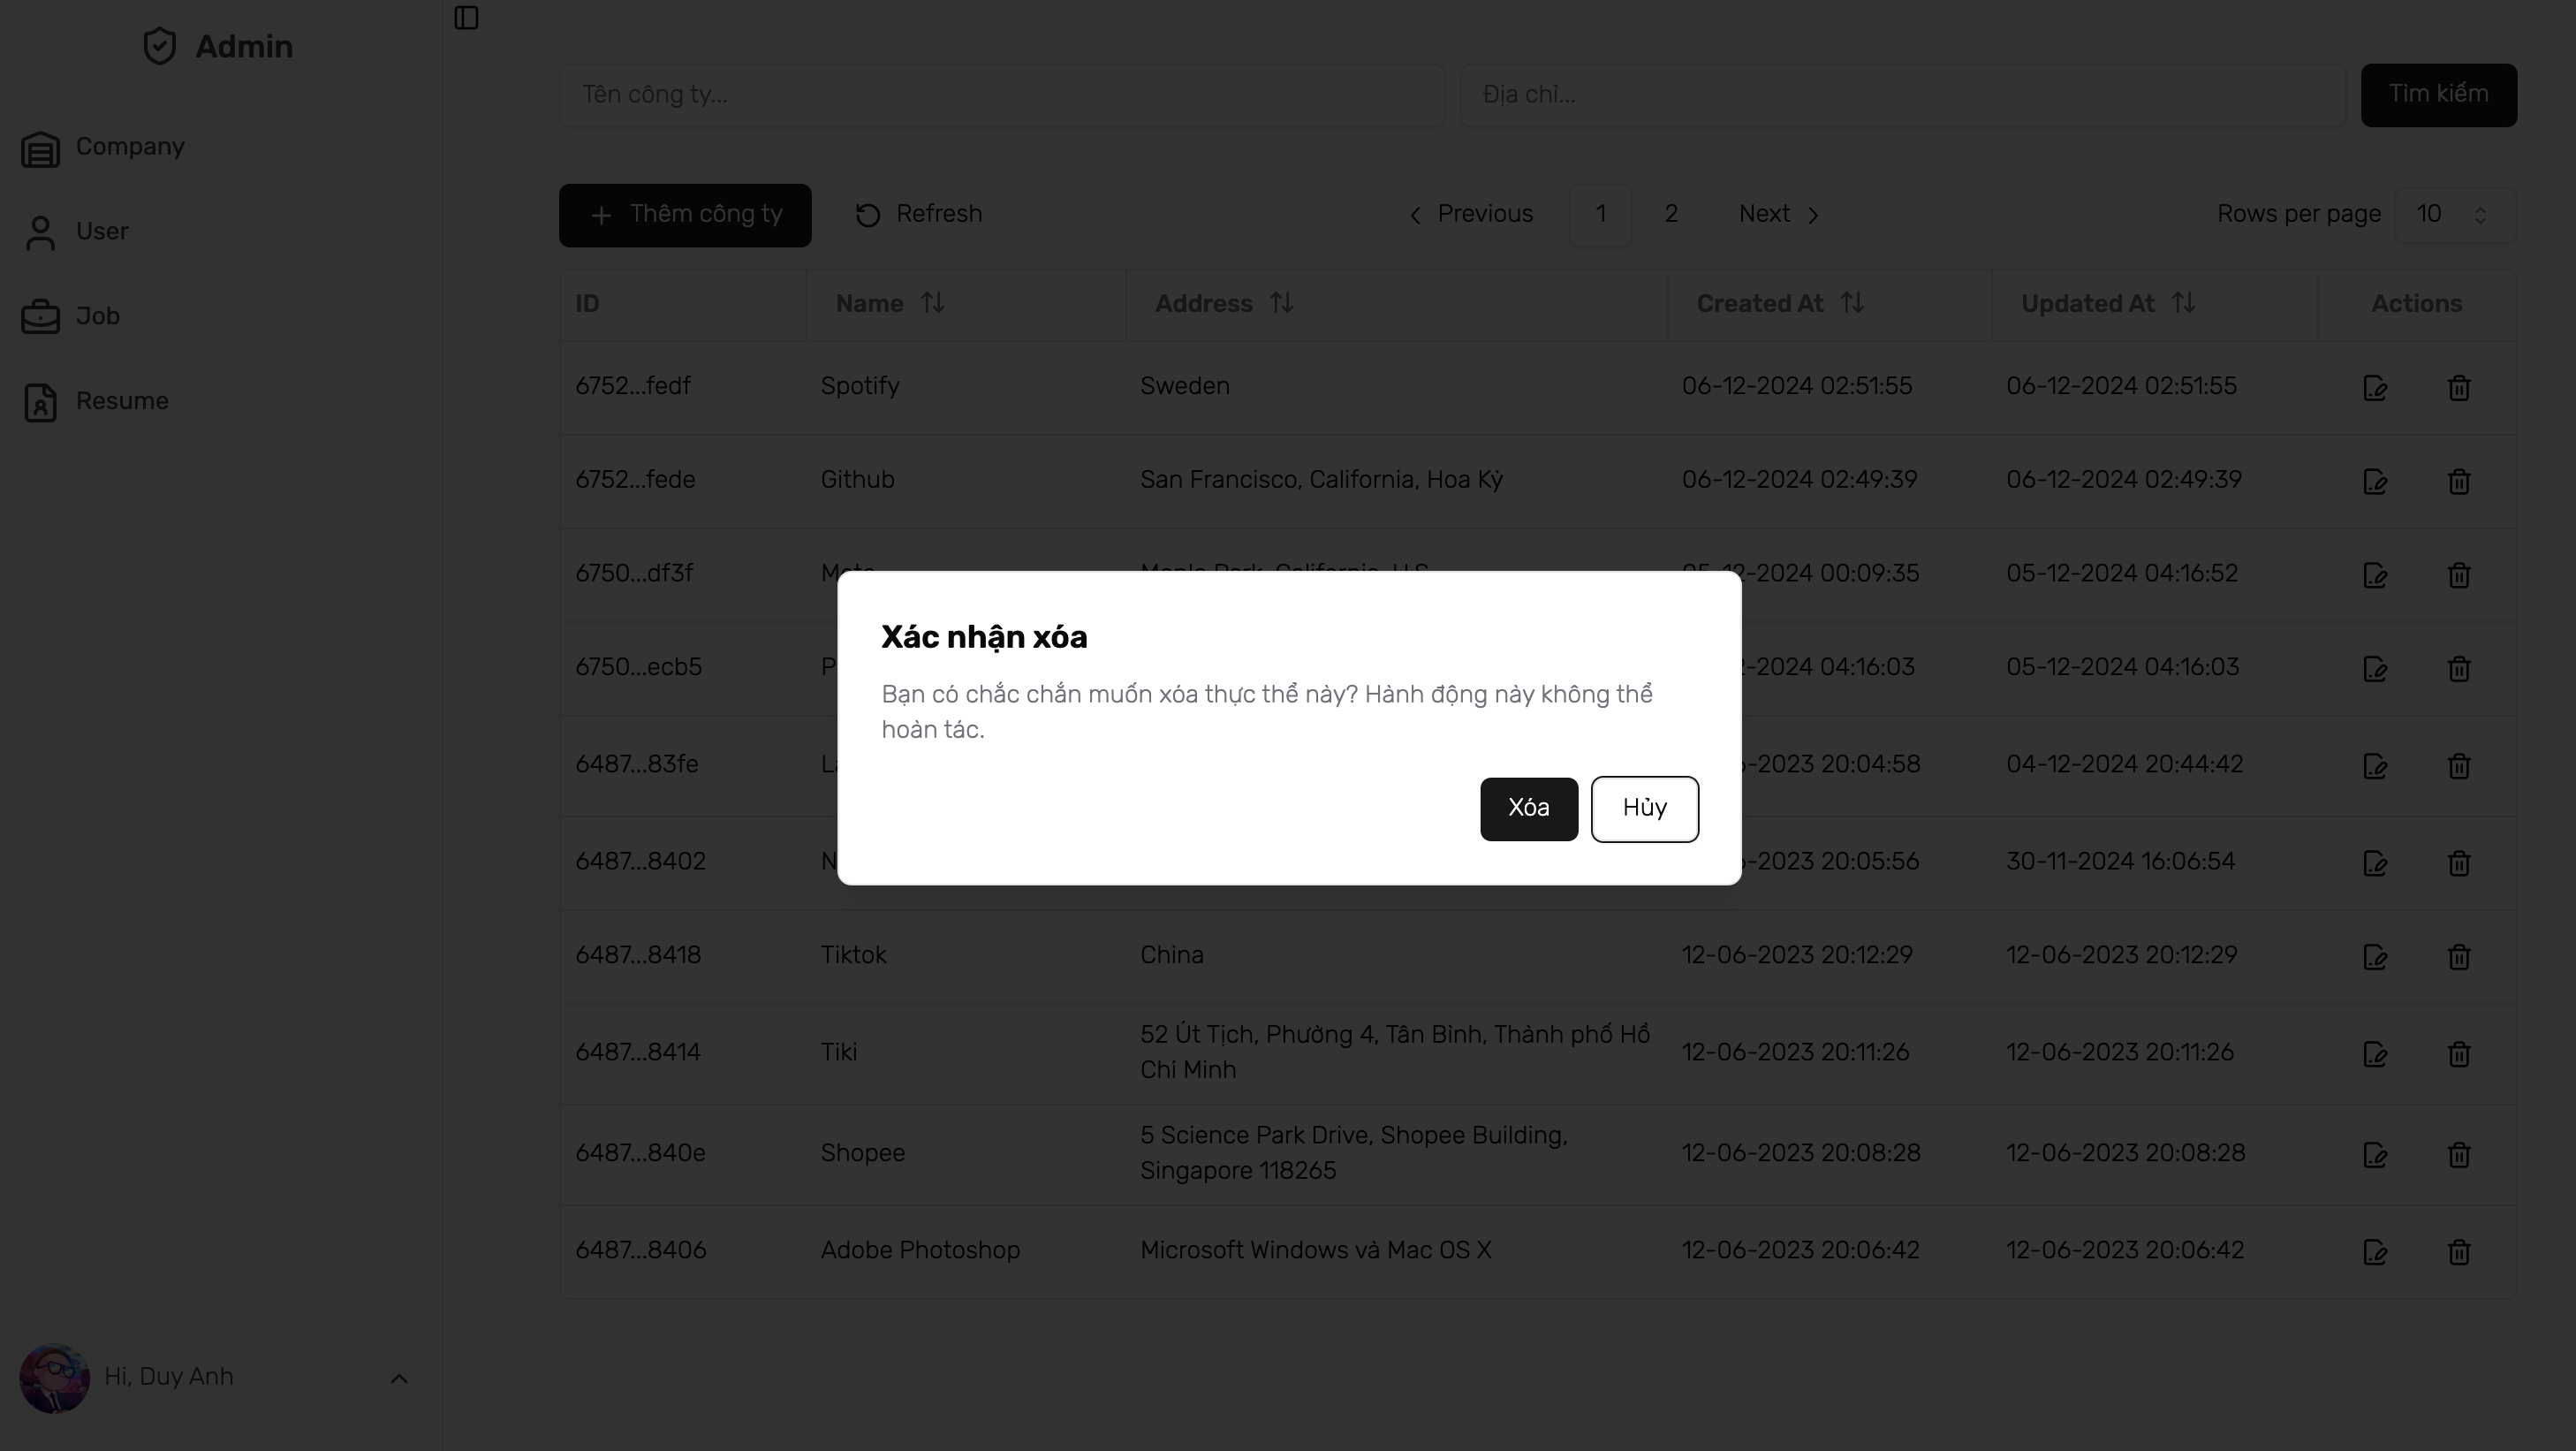
\includegraphics[width=\linewidth]{DBMS-Application/Images/delete-company.png}
        \caption{Trang quản lý công ty - Xoá công ty}
        \label{fig:enter-label}
    \end{figure}
\end{itemize}

% \subsubsection{Giao diện Admin - Quản lý người dùng}

Tương tự với trang quản lý công ty và quản lý công việc, trang quản lý người dùng cũng sử dụng các loại truy vấn sau để hỗ trợ cho các thao tác CRUD:

\begin{itemize}
    \item \textbf{Query with single/composite condition}: Để fetch lên dữ liệu toàn bộ người dùng trong hệ thống theo cơ chế phân trang và một số điều kiện như \textbf{Tên người dùng}, \textbf{Email}
    \begin{figure}[H]
        \centering
        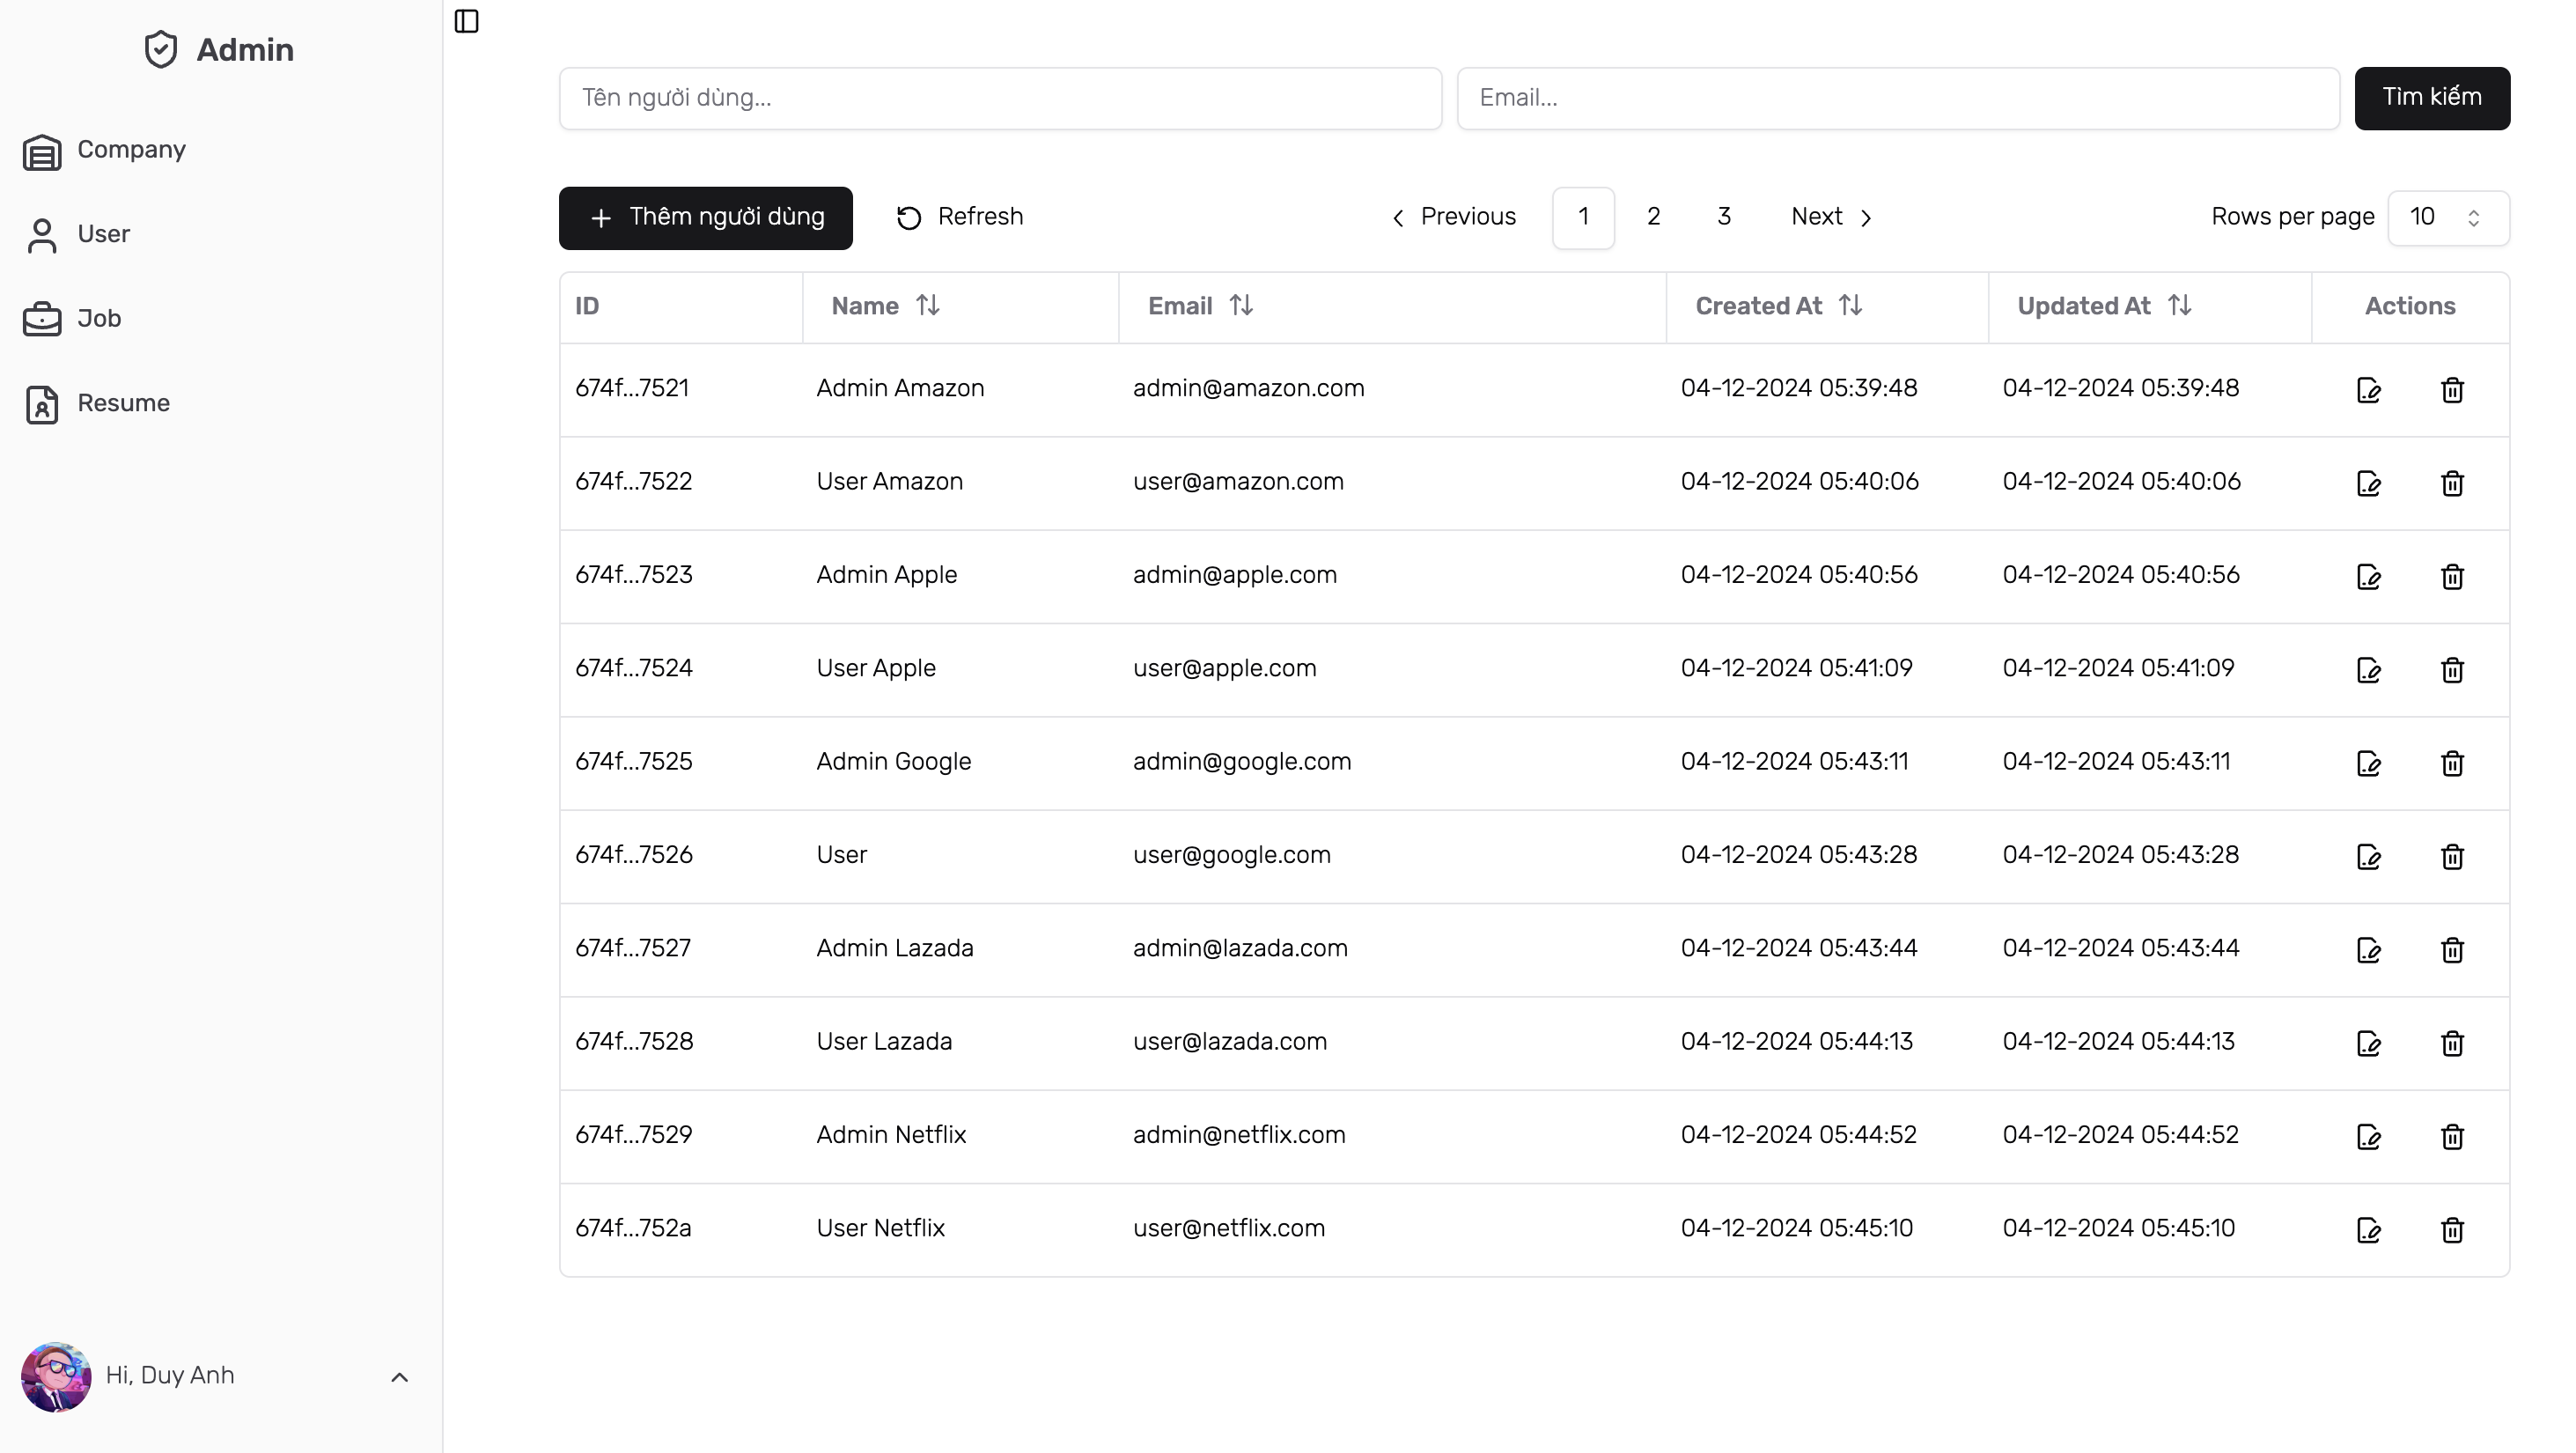
\includegraphics[width=\linewidth]{DBMS-Application/Images/admin-user.png}
        \caption{Trang quản lý người dùng - Danh sách người dùng trong hệ thống}
        \label{fig:enter-label}
    \end{figure}
    
    \item \textbf{Insert}: Thêm mới một người dùng
    \begin{figure}[H]
        \centering
        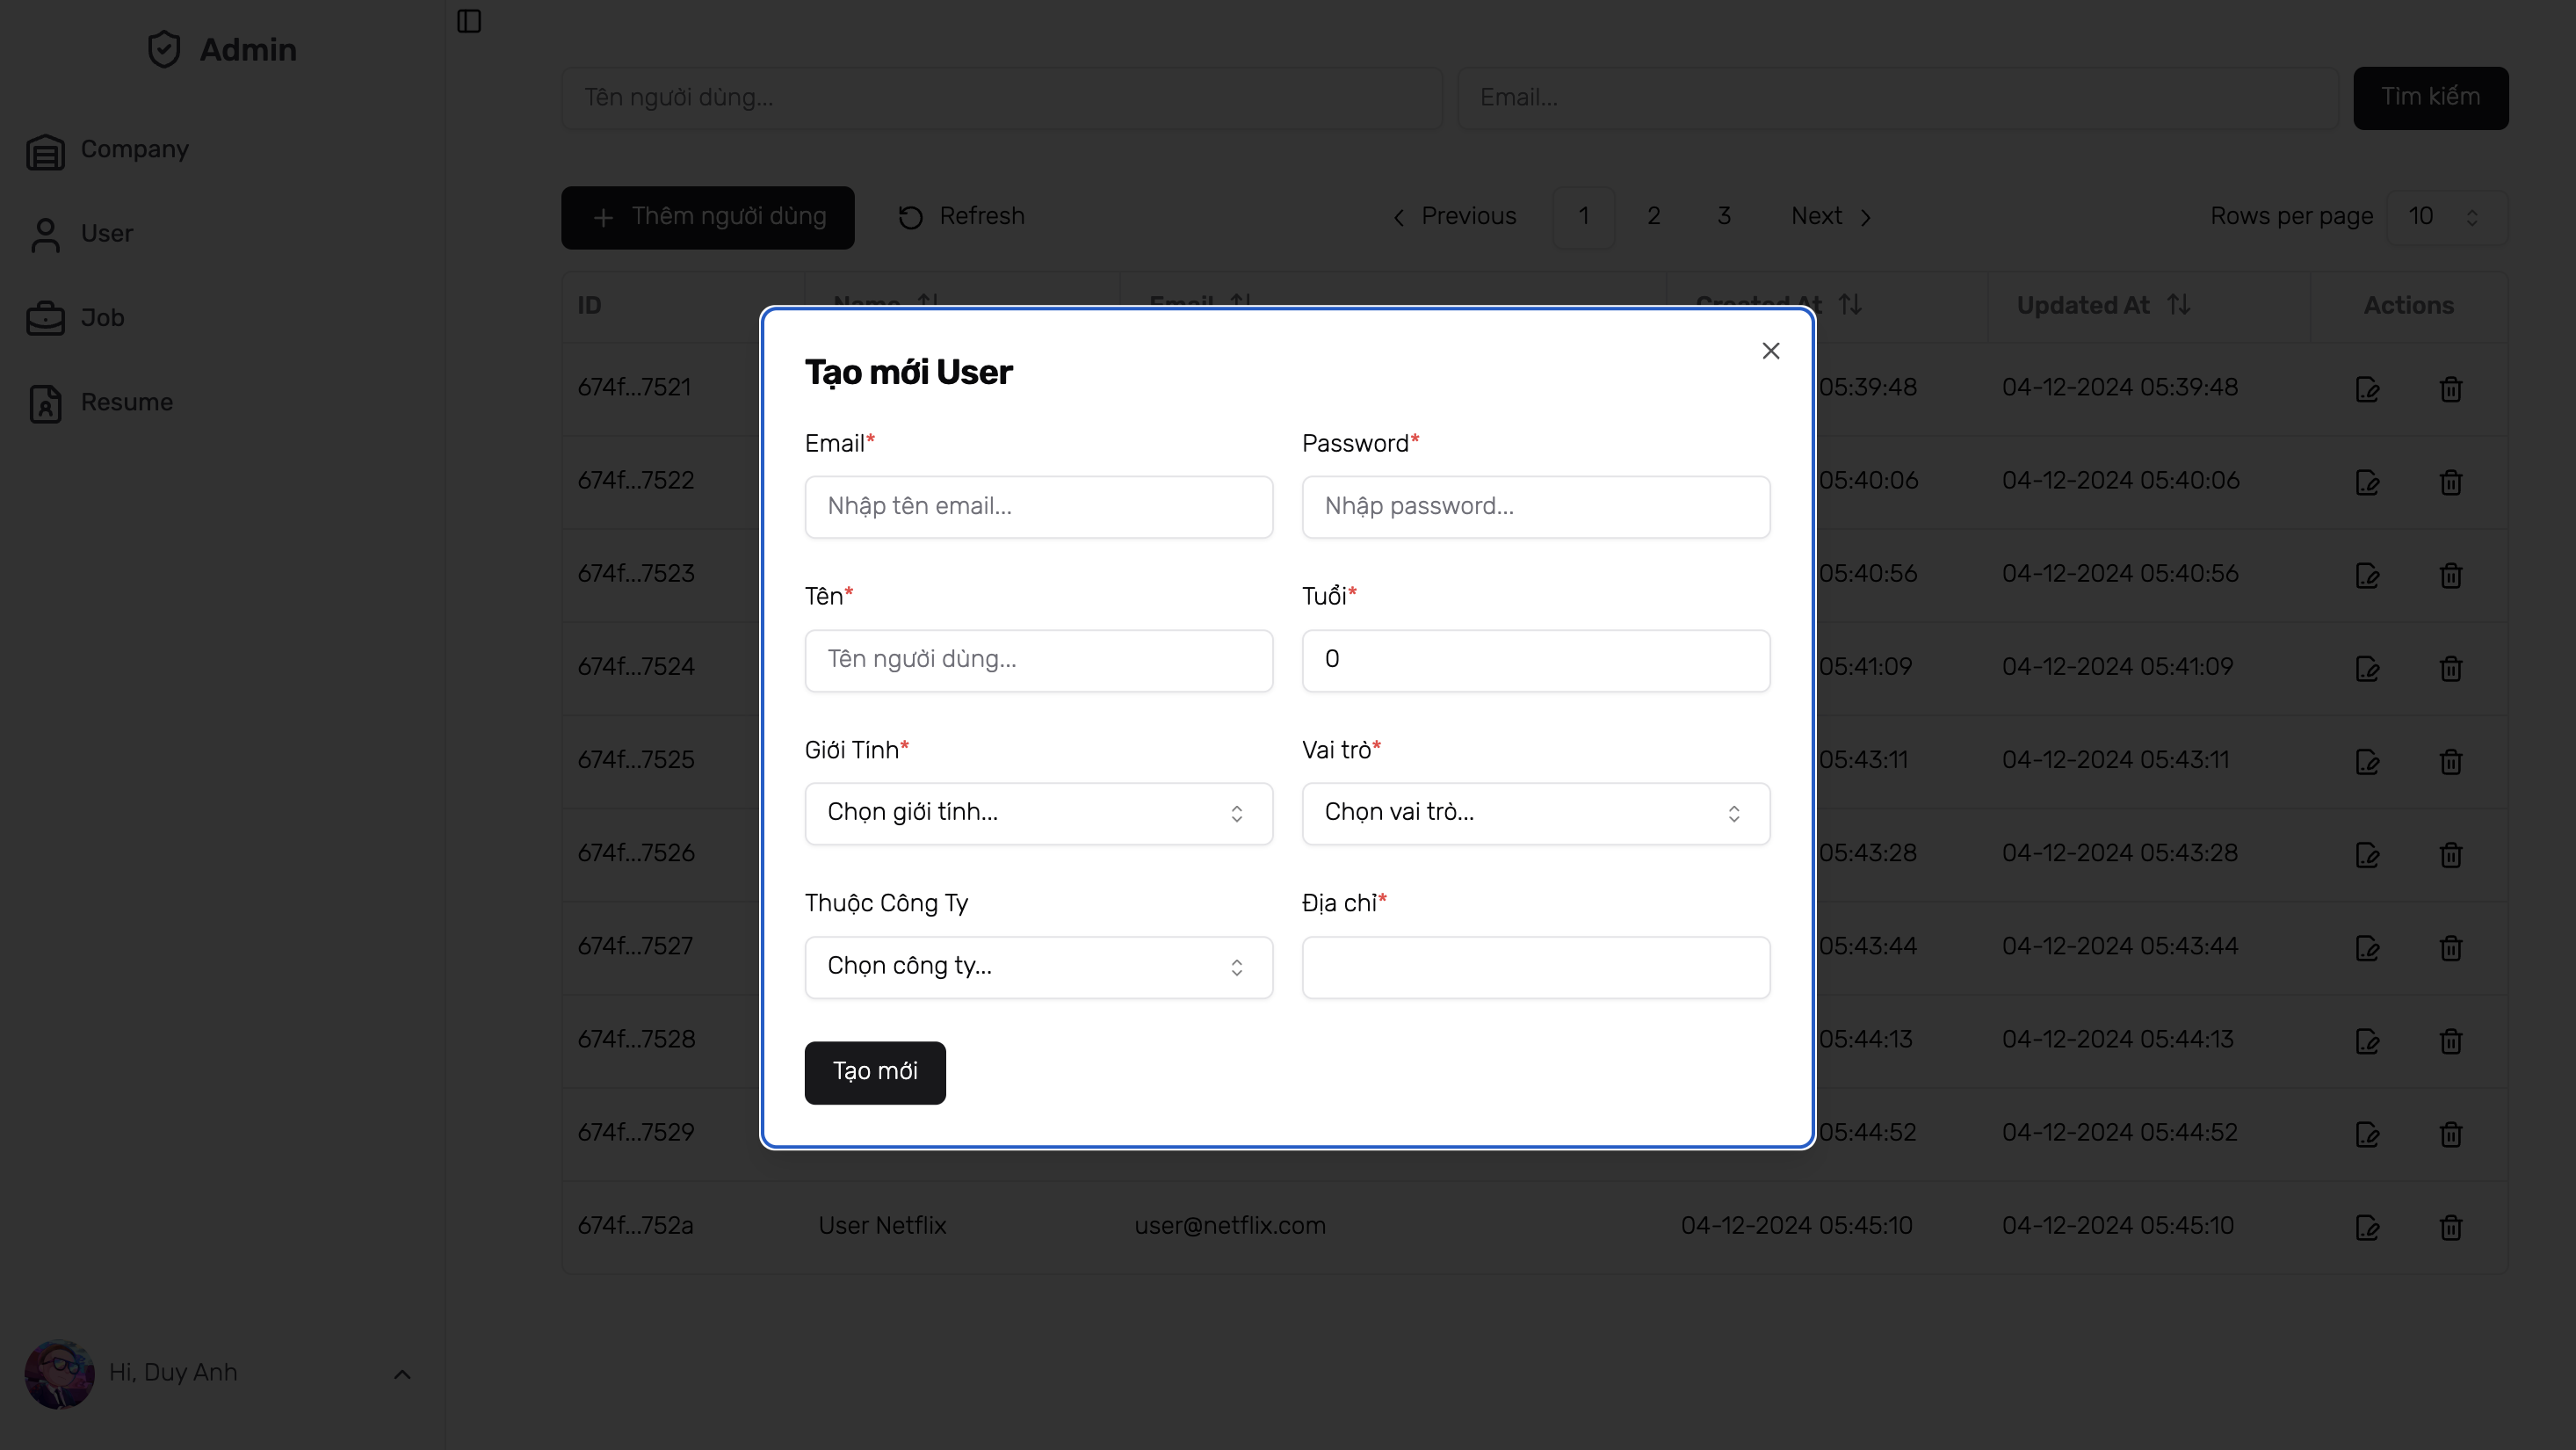
\includegraphics[width=\linewidth]{DBMS-Application/Images/create-user.png}
        \caption{Trang quản lý người dùng - Thêm mới người dùng}
        \label{fig:enter-label}
    \end{figure}

    \item \textbf{Update}: Cập nhật/chỉnh sửa thông tin người dùng cụ thể
    \begin{figure}[H]
        \centering
        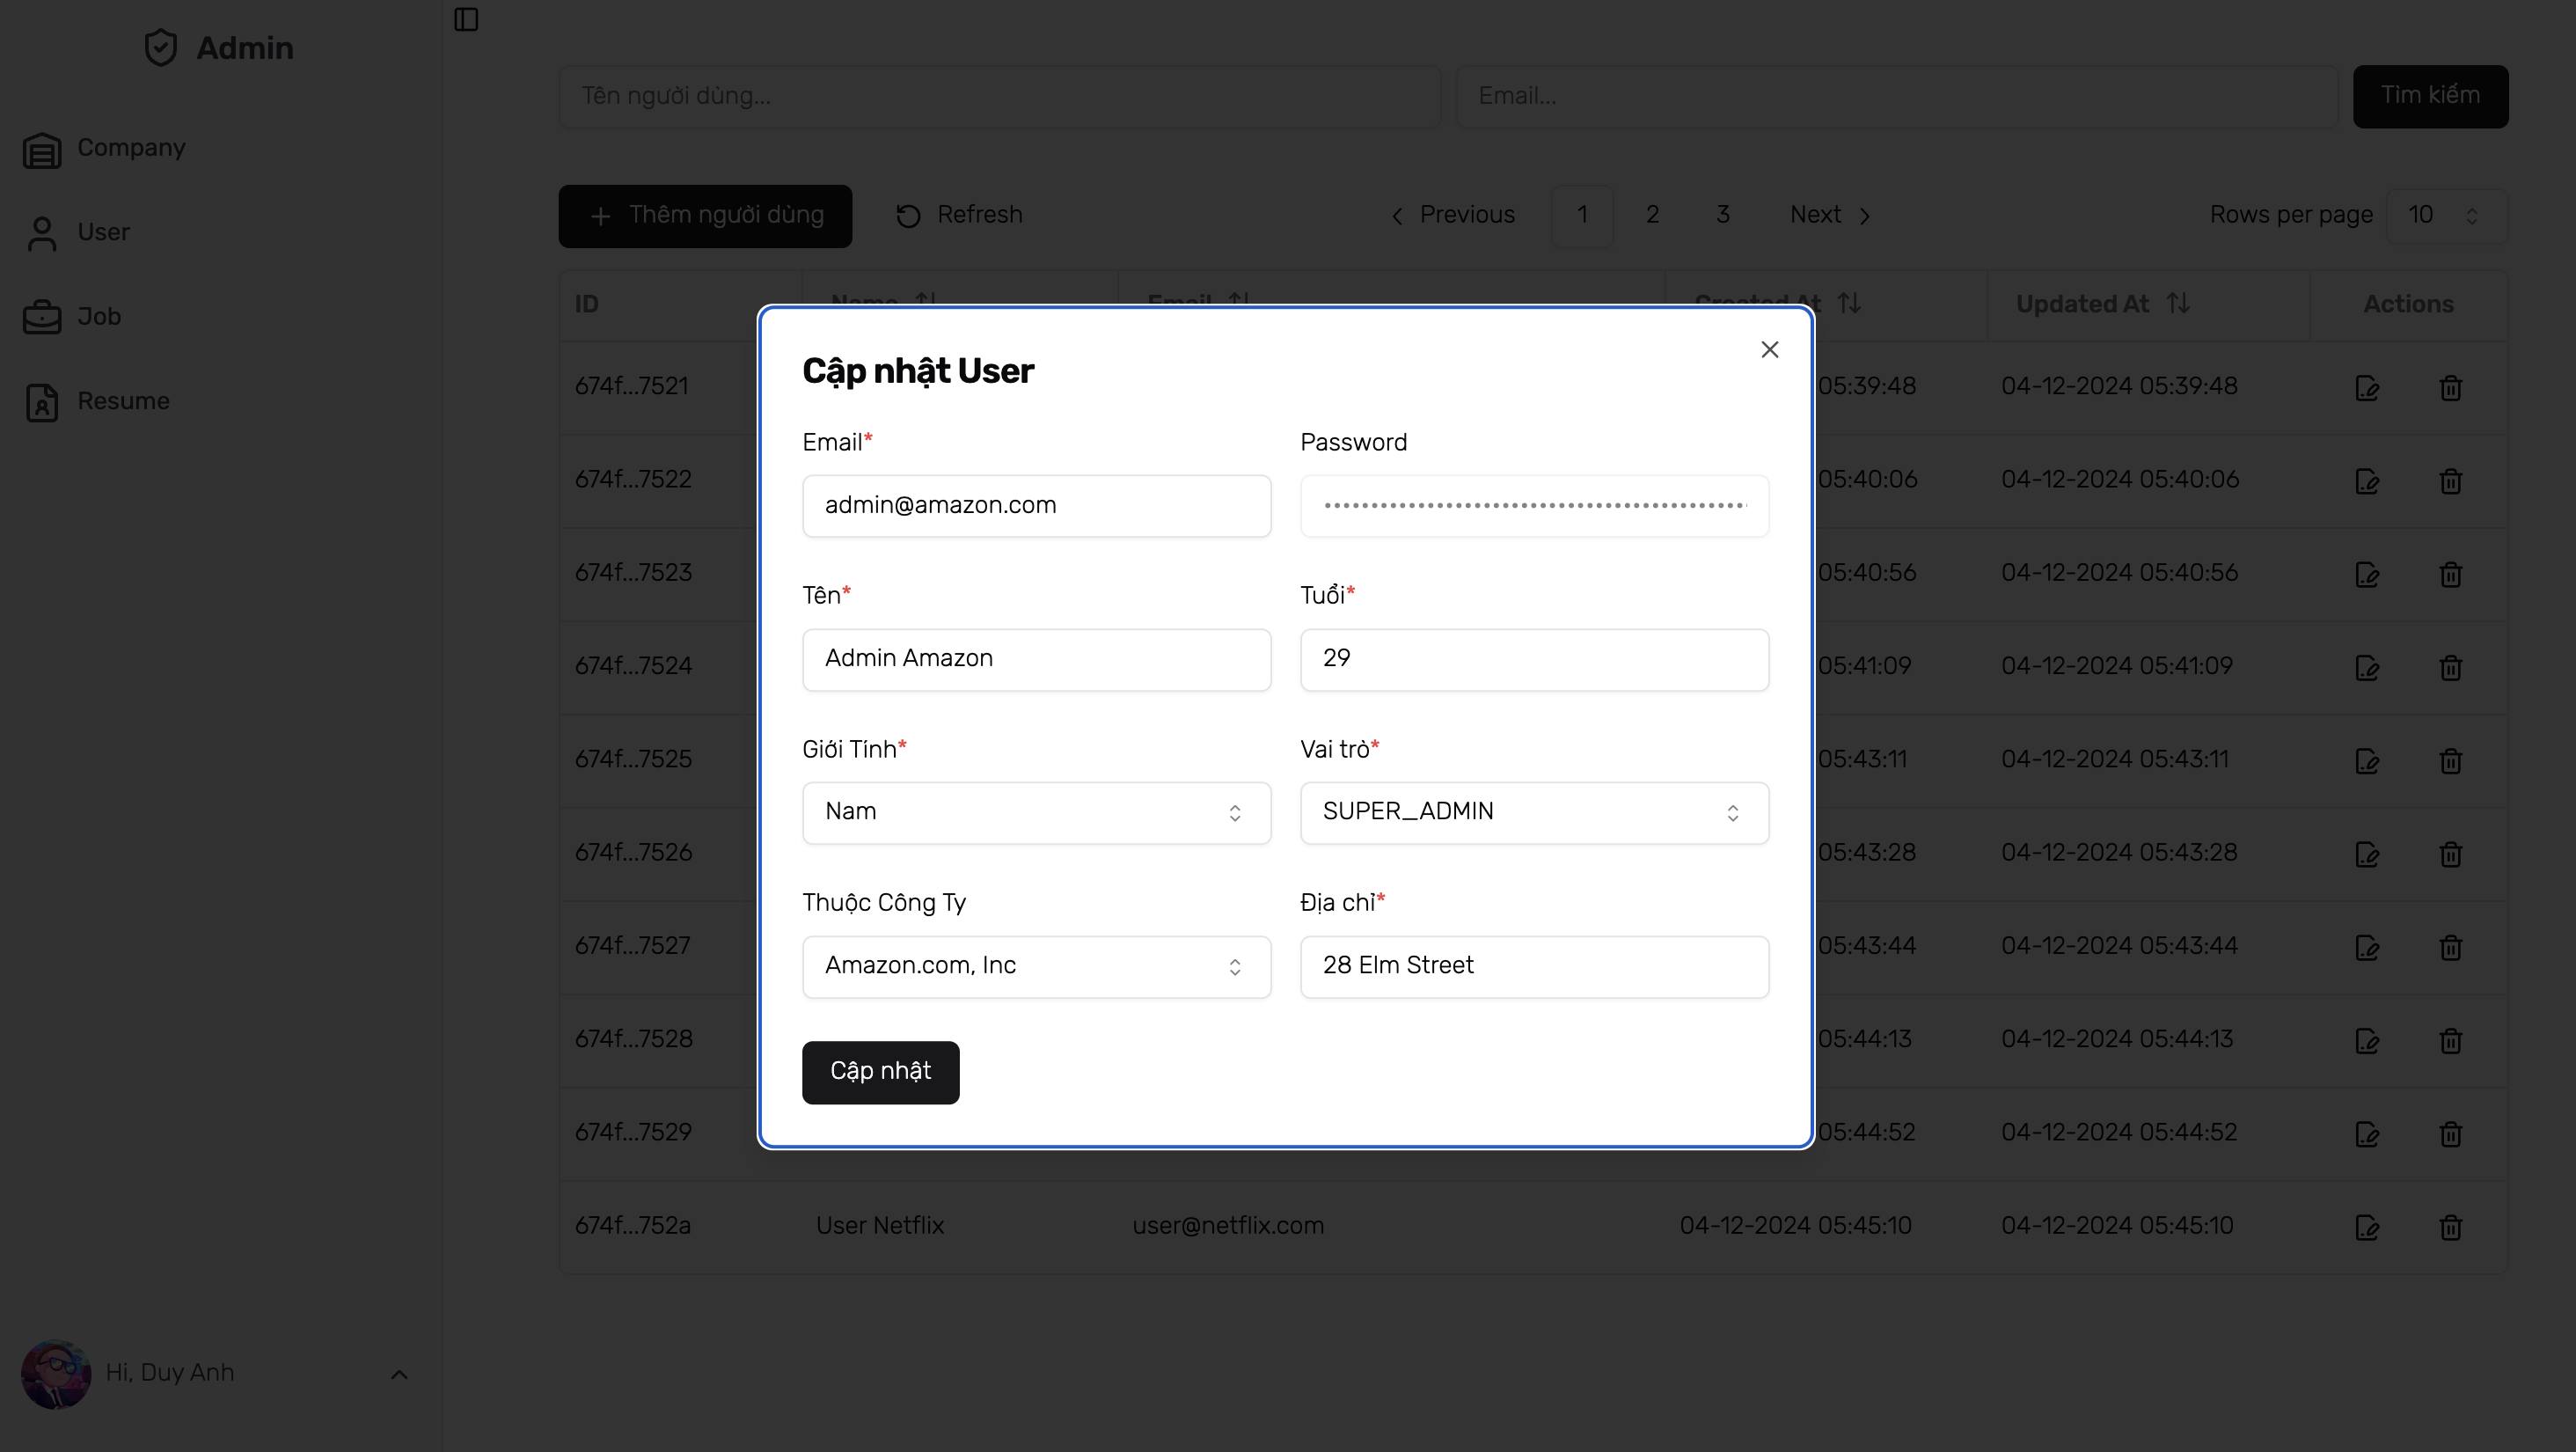
\includegraphics[width=\linewidth]{DBMS-Application/Images/update-user.png}
        \caption{Trang quản lý người dùng - Cập nhật thông tin người dùng}
        \label{fig:enter-label}
    \end{figure}

    \item \textbf{Delete}: Xoá người dùng
    \begin{figure}[H]
        \centering
        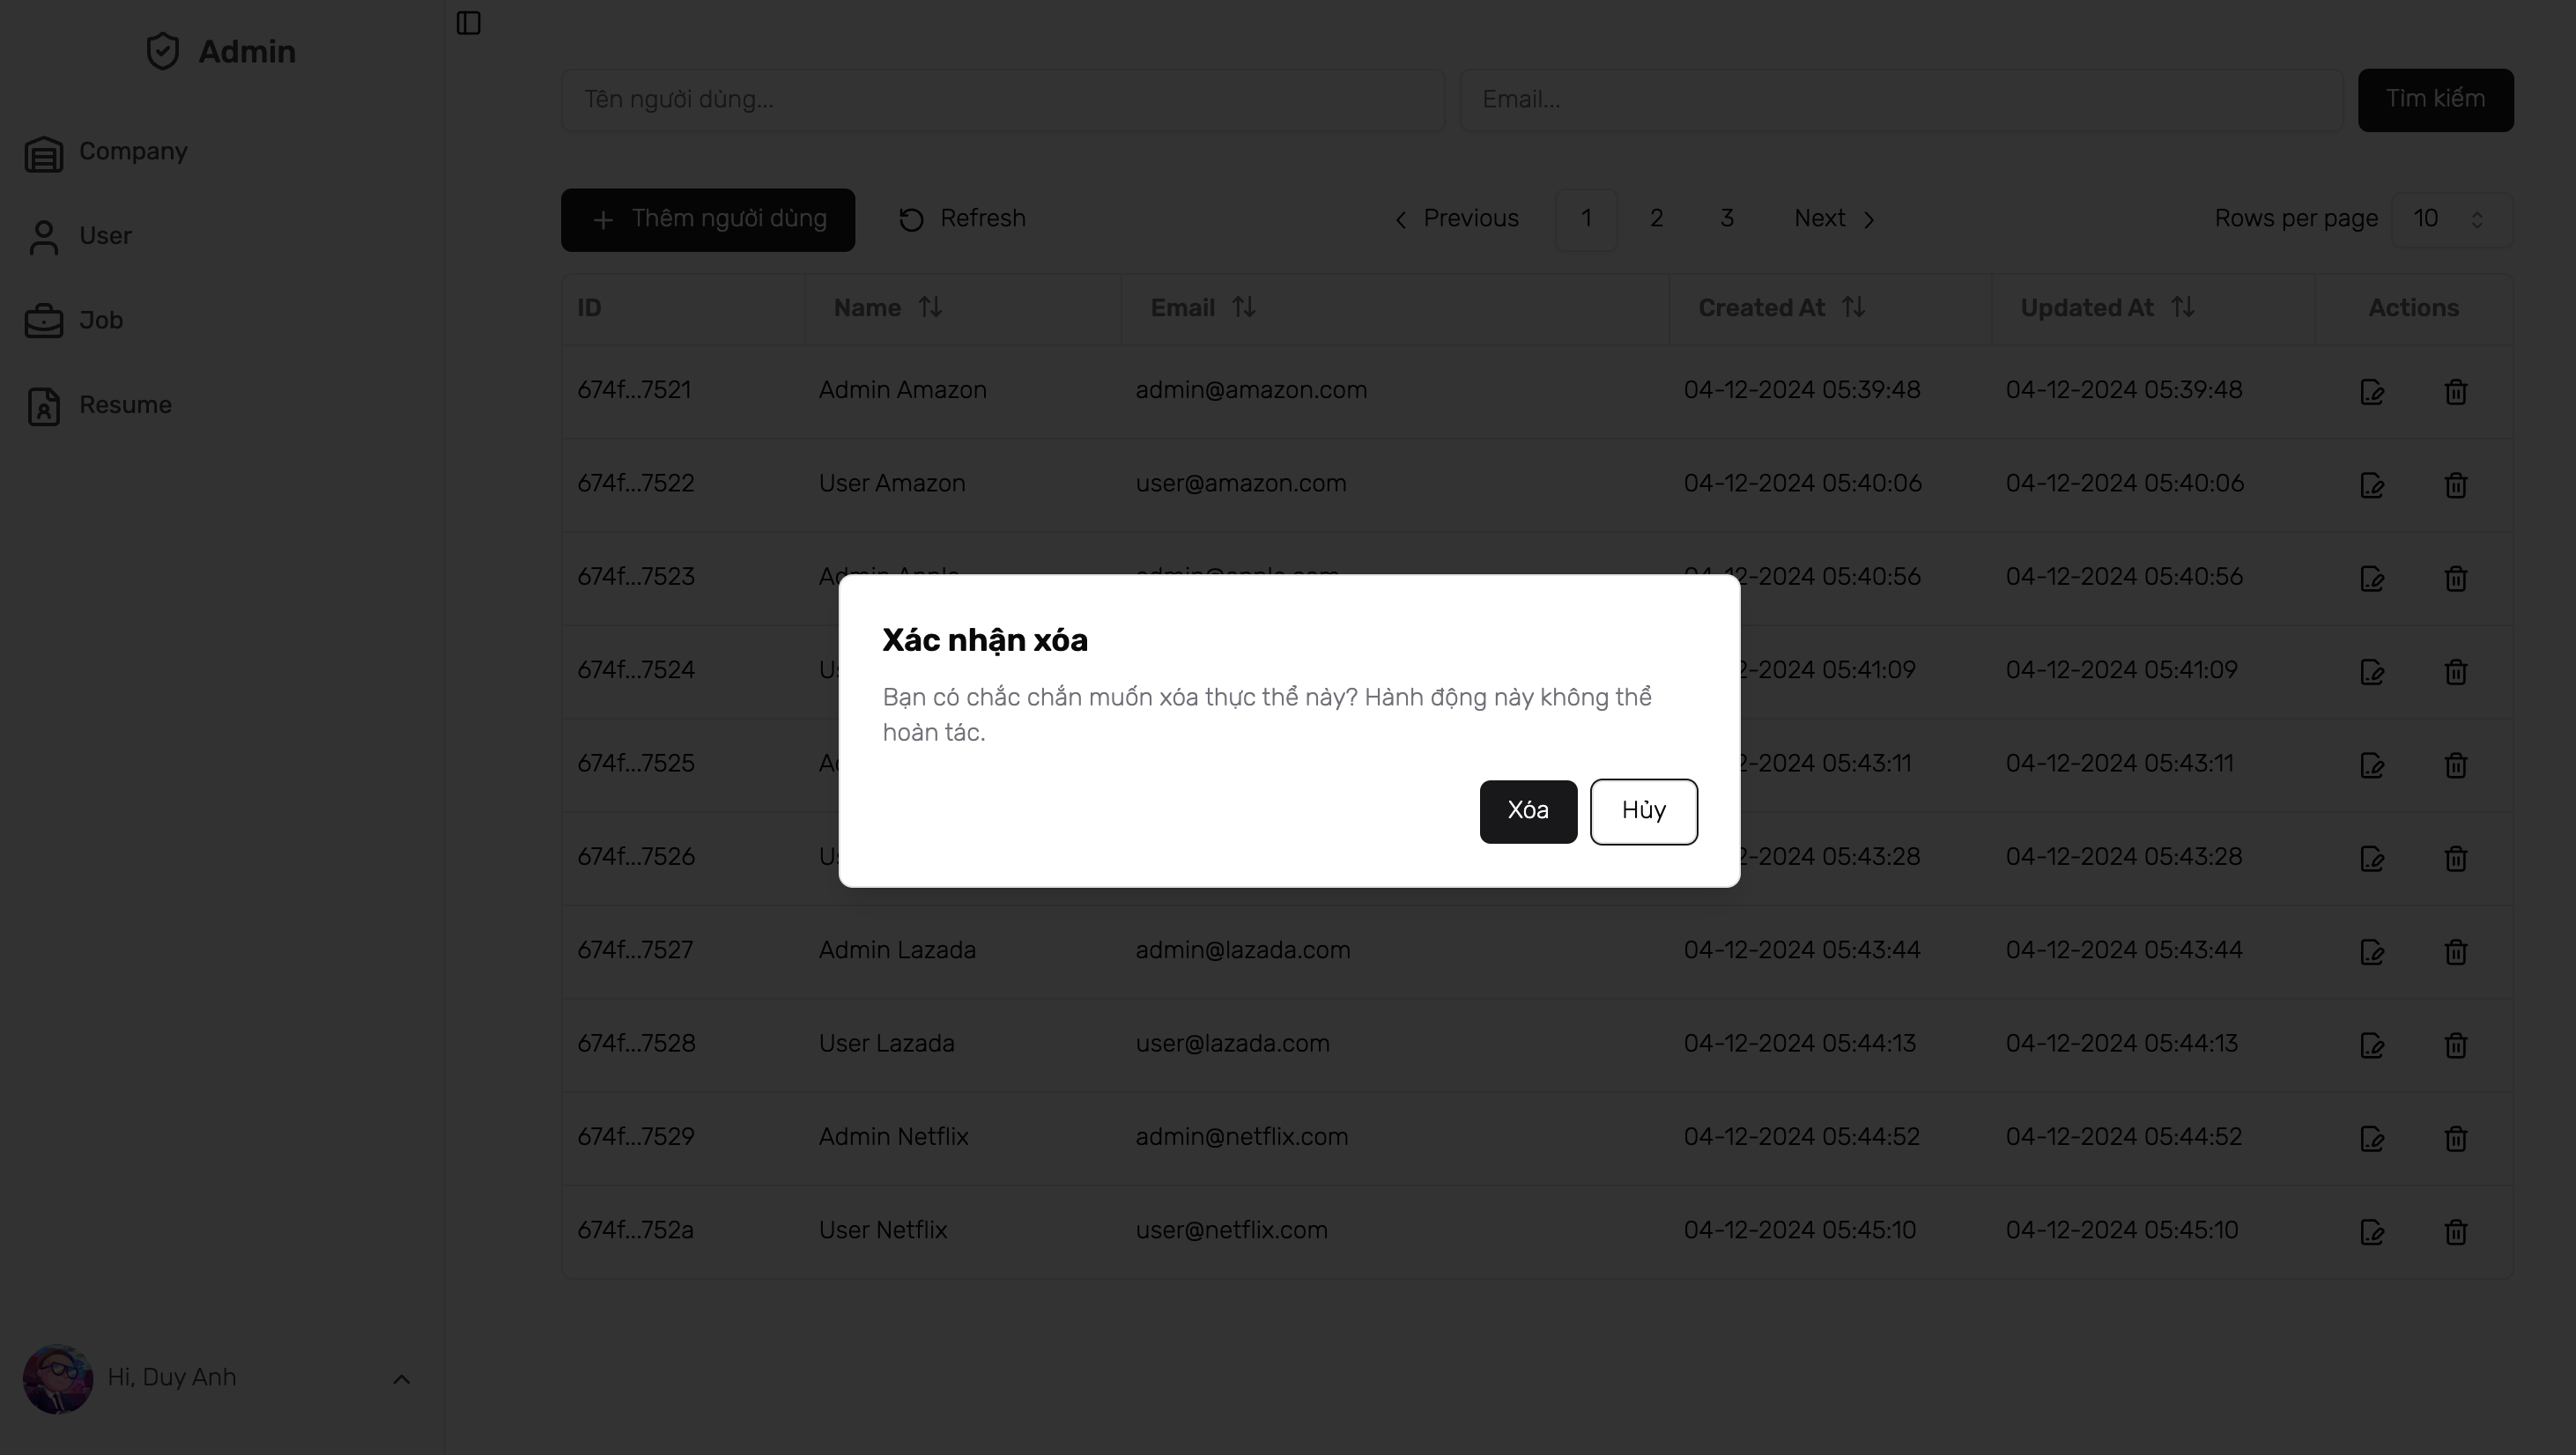
\includegraphics[width=\linewidth]{DBMS-Application/Images/delete-user.png}
        \caption{Trang quản lý người dùng - Xoá người dùng}
        \label{fig:enter-label}
    \end{figure}
\end{itemize}

% \subsubsection{Giao diện Admin - Quản lý hồ sơ ứng tuyển}

\begin{itemize}
    \item \textbf{Query with composite condition}: Để fetch lên dữ liệu toàn bộ hồ sơ ứng tuyển trong hệ thống theo cơ chế phân trang
    \begin{figure}[H]
        \centering
        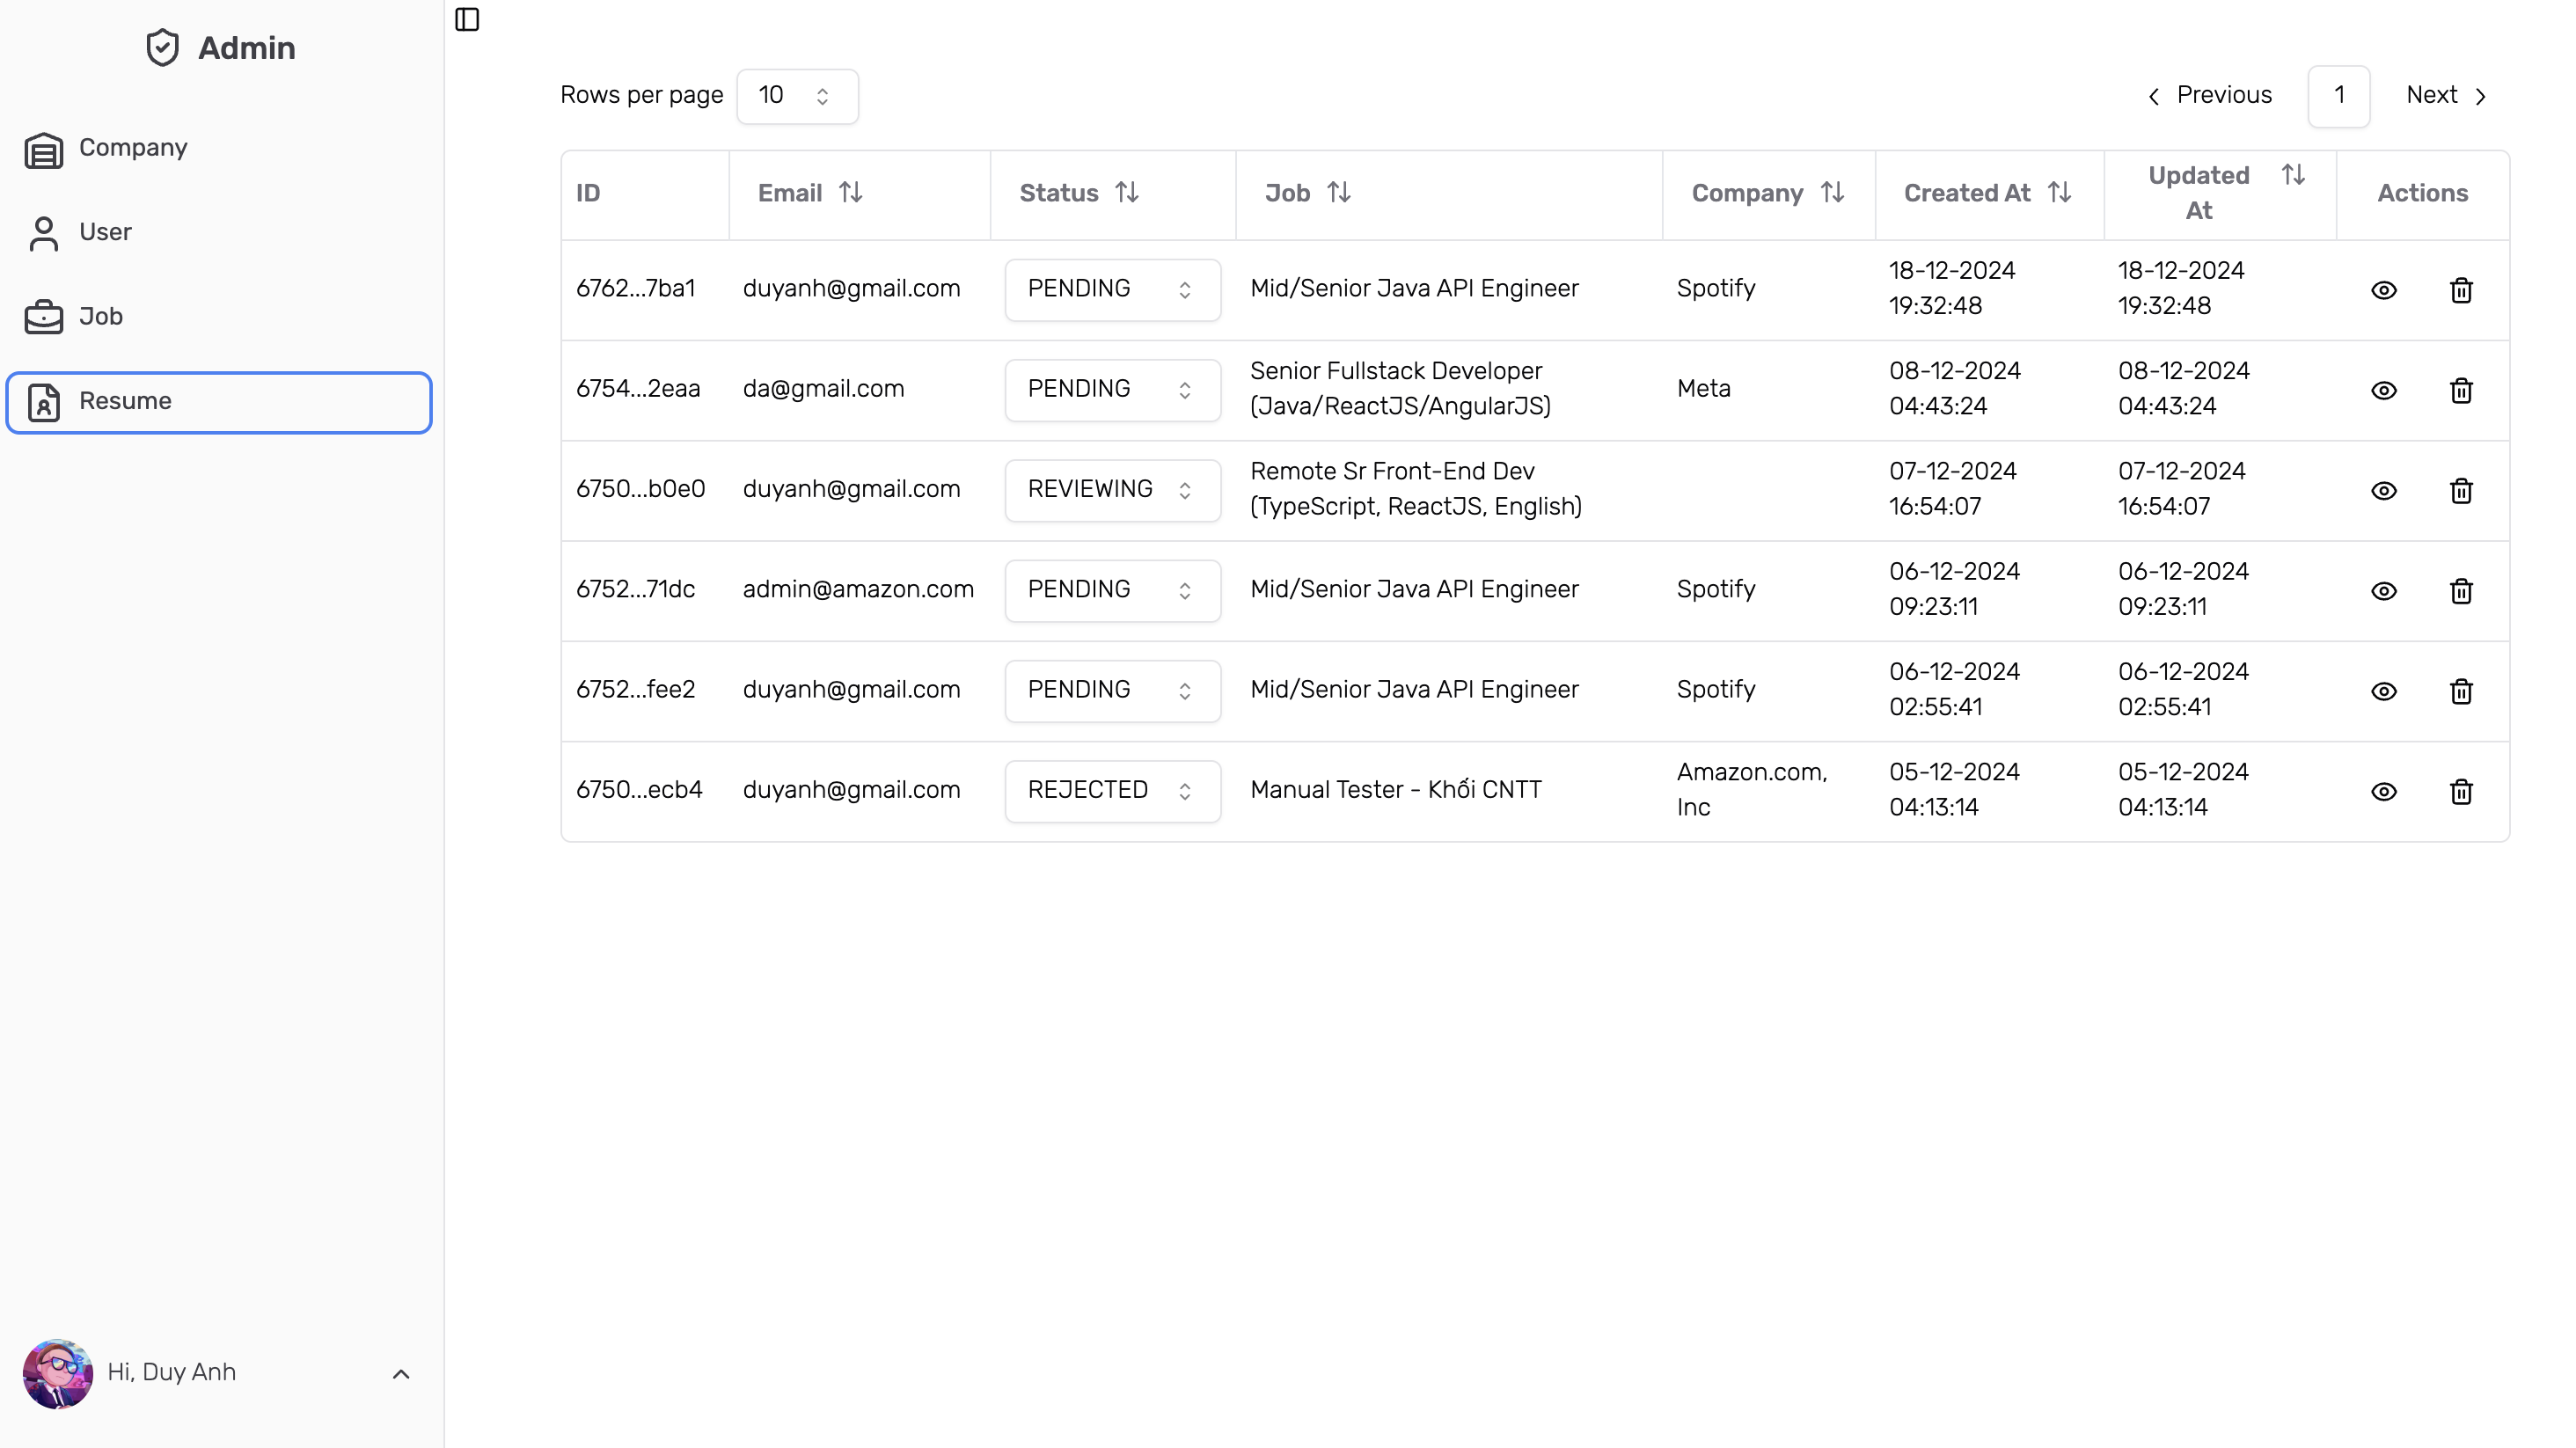
\includegraphics[width=\linewidth]{DBMS-Application/Images/admin-resume.png}
        \caption{Trang quản lý hồ sơ ứng tuyển - Danh sách hồ sơ ứng tuyển trong hệ thống}
        \label{fig:enter-label}
    \end{figure}

    \item \textbf{Update}: Cập nhật thông tin của hồ sơ ứng tuyển, cụ thể là cập nhật \textbf{trạng thái}
    \begin{figure}[H]
        \centering
        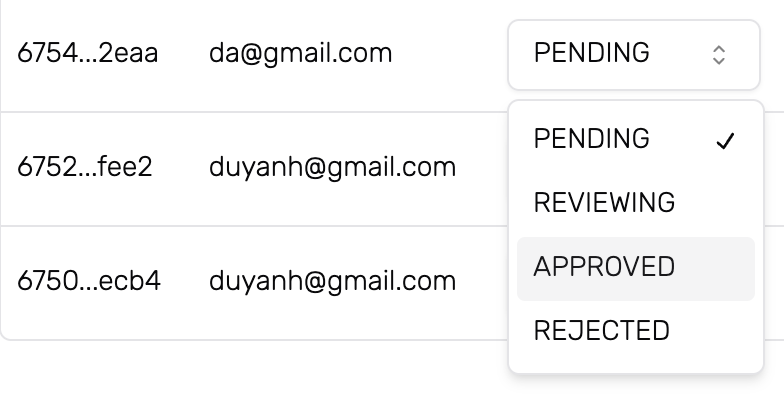
\includegraphics[width=.5\linewidth]{DBMS-Application/Images/update-status-resume.png}
        \caption{Trang quản lý hồ sơ ứng tuyển - Chọn trạng thái mới cho hồ sơ}
        \label{fig:enter-label}
    \end{figure}

    \begin{figure}[H]
        \centering
        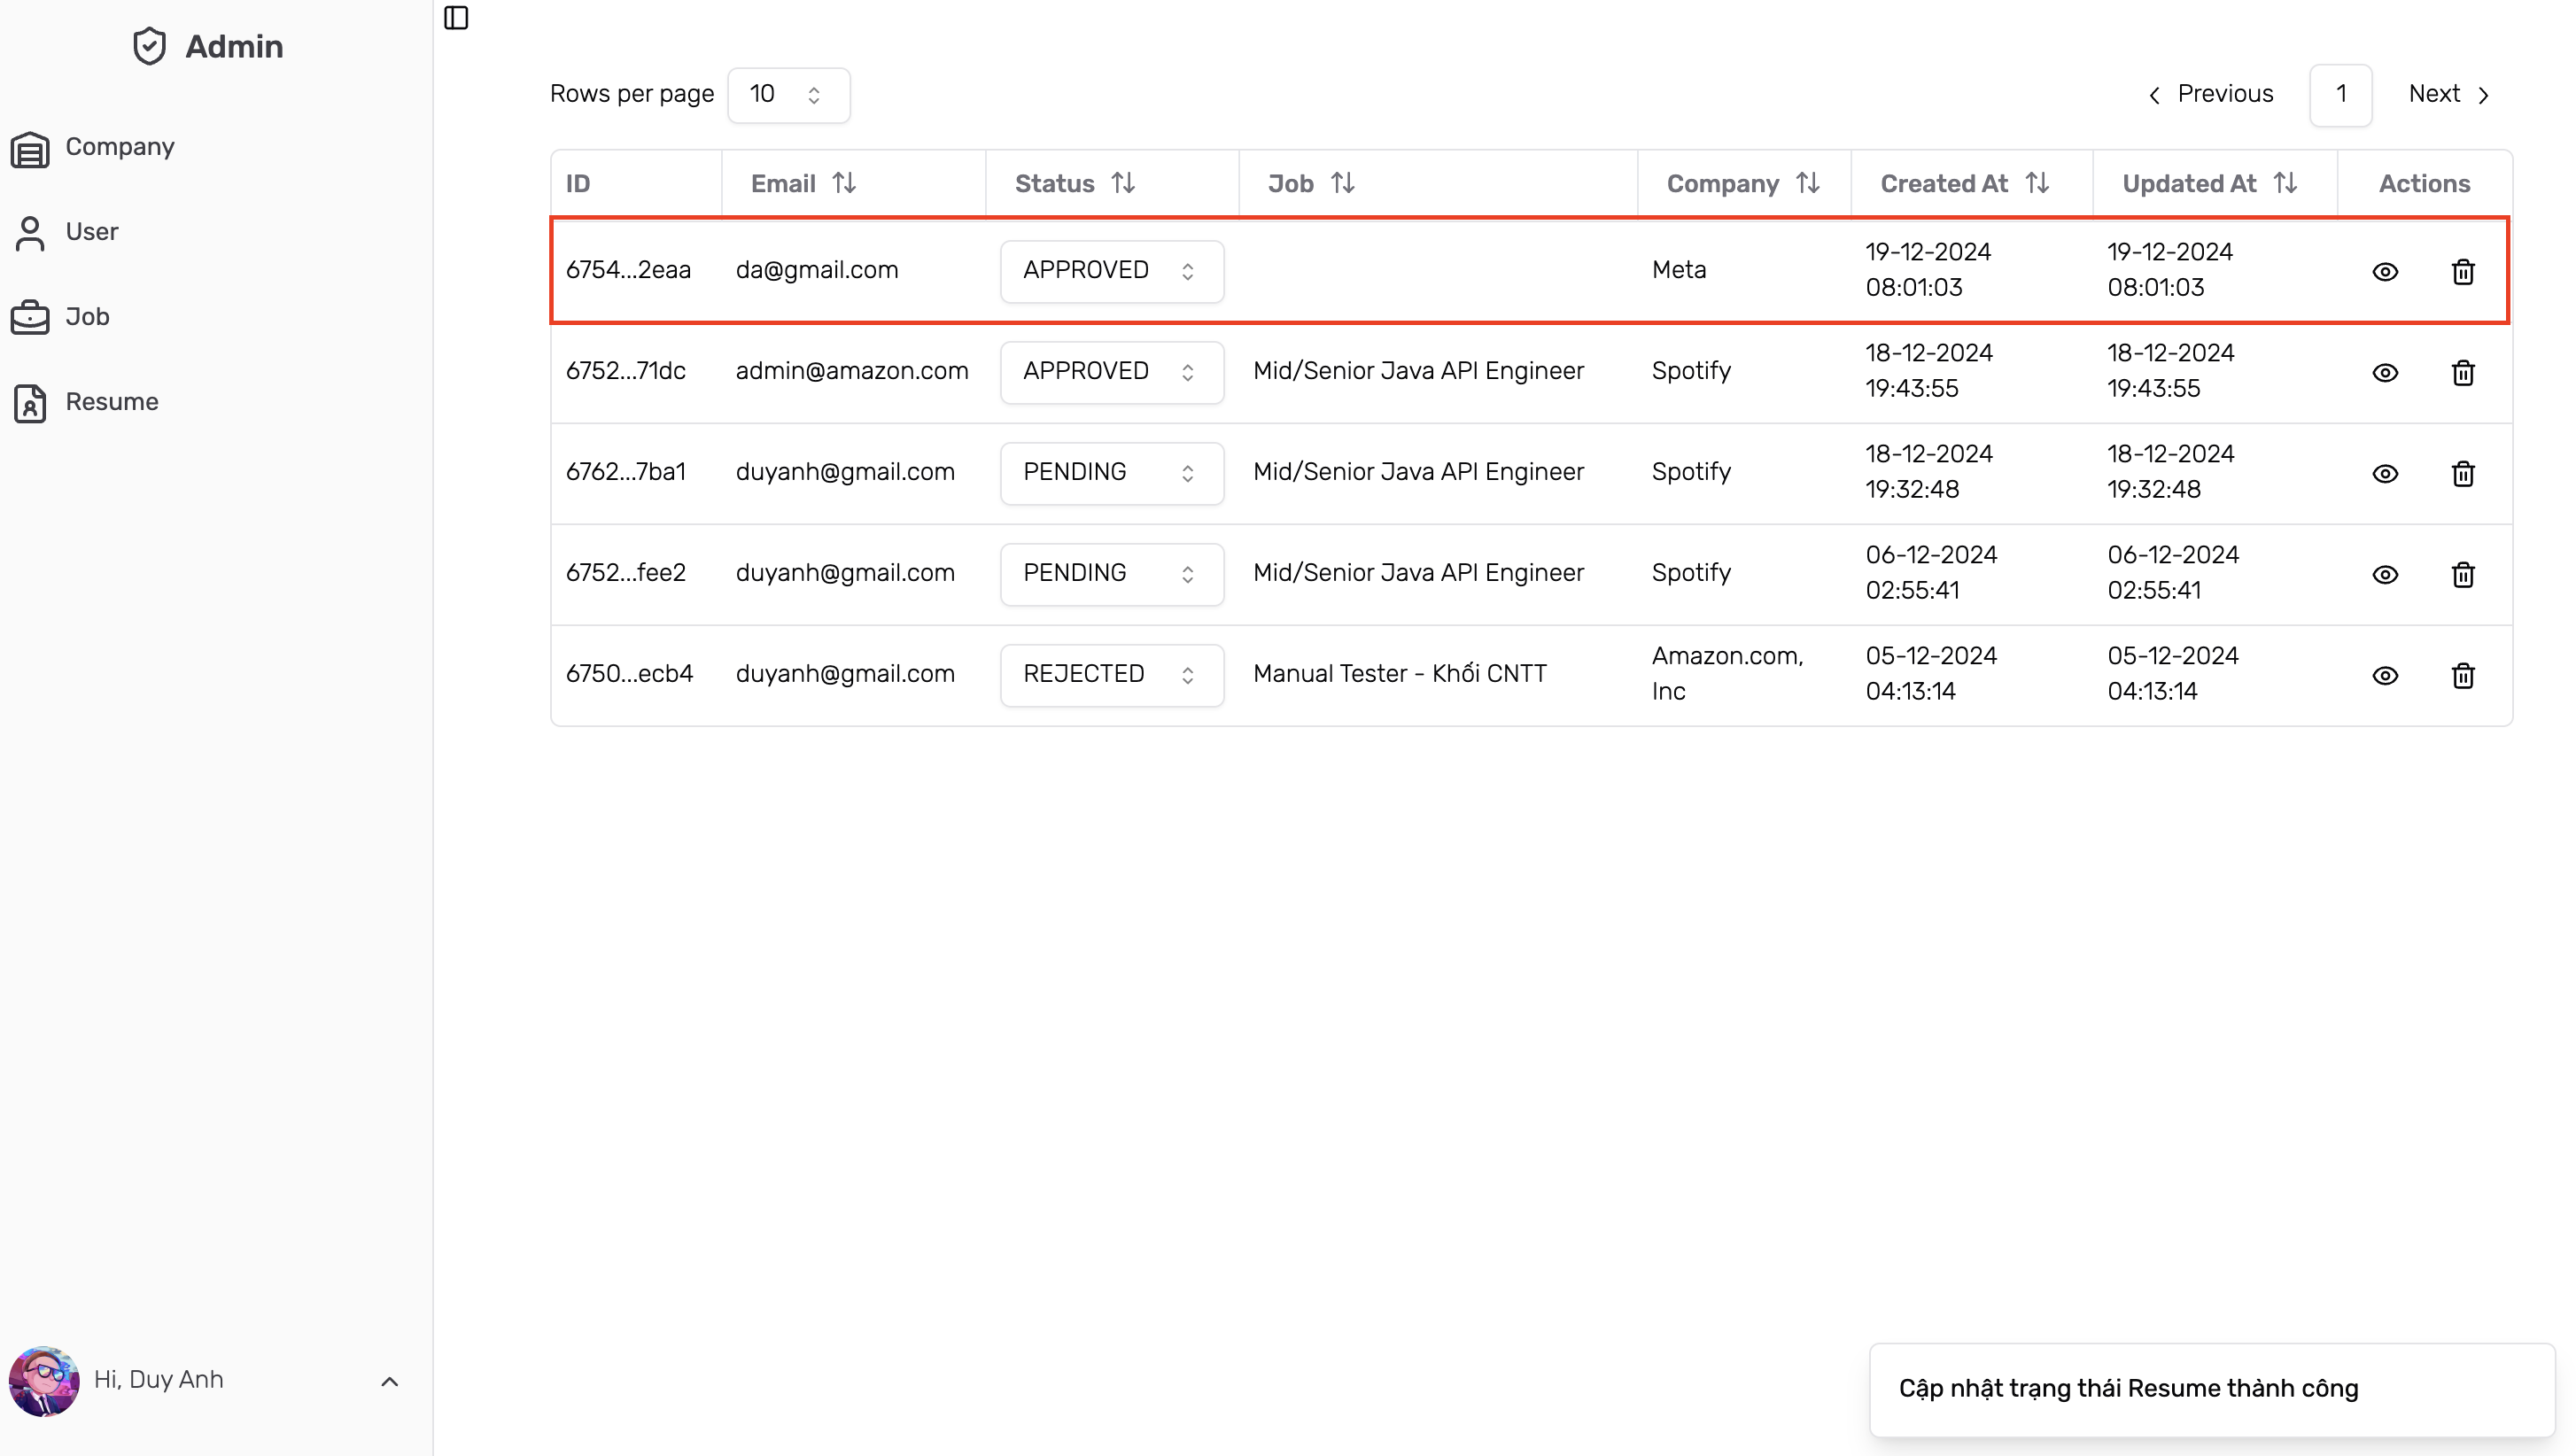
\includegraphics[width=\linewidth]{DBMS-Application/Images/update-resume-successfully.png}
        \caption{Trang quản lý hồ sơ ứng tuyển - Cập nhật trạng thái của hồ sơ ứng tuyển thành công}
        \label{fig:enter-label}
    \end{figure}
    
    \item \textbf{Delete}: Xoá hồ sơ ứng tuyển chỉ định
    \begin{figure}[H]
        \centering
        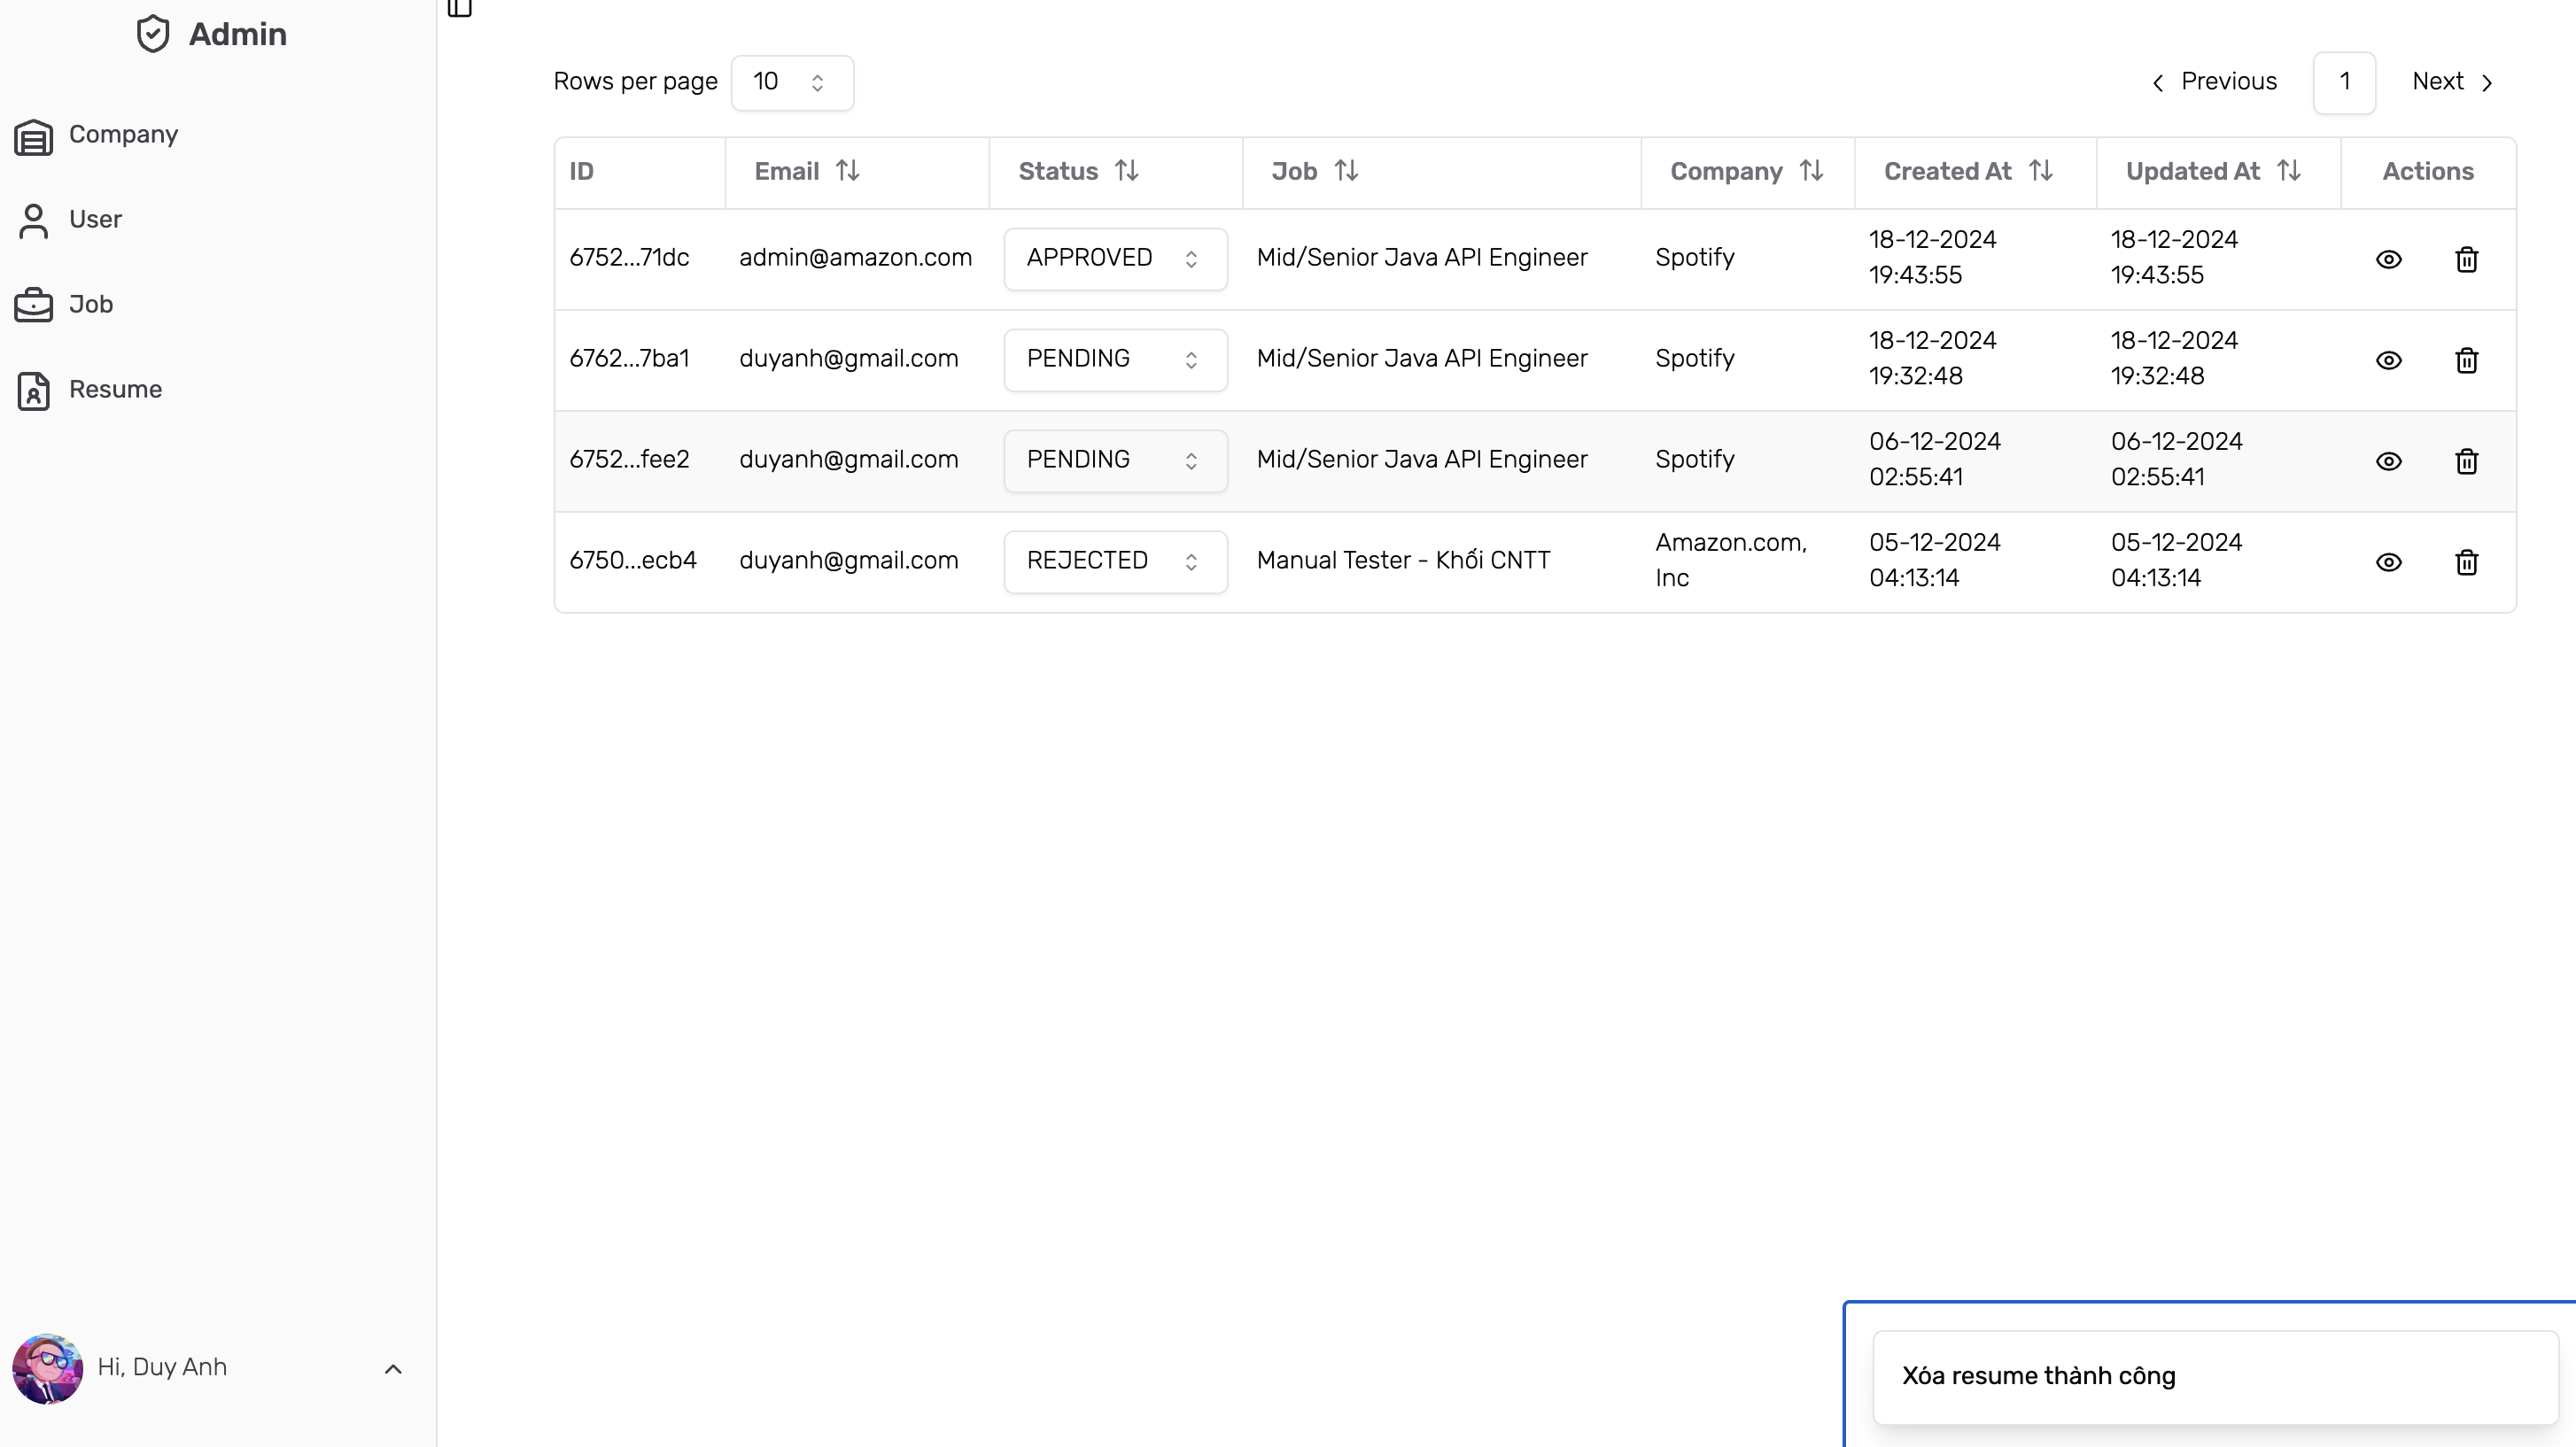
\includegraphics[width=\linewidth]{DBMS-Application/Images/delete-resume.png}
        \caption{Trang quản lý hồ sơ ứng tuyển - Xoá hồ sơ ứng tuyển}
        \label{fig:enter-label}
    \end{figure}
\end{itemize}
\subsubsection{Kết nối Backend - Database}

Trong hệ thống backend, nhóm tạo một module riêng biệt được dùng cho việc quản lý kết nối và truy cập đến cơ sở dữ liệu là \textbf{MongoModule}. Trong module này, \textbf{MongoService} là service được nhóm định nghĩa nhằm khởi tạo kết nối với database của hệ thống khi module khởi chạy và cung cấp đối tượng \texttt{Db} (đại diện cho cơ sở dữ liệu của hệ thống), thông qua một phương thức chung \texttt{getDatabase} cho các service khác sử dụng.

\begin{lstlisting}
import { Injectable, OnModuleDestroy, OnModuleInit } from '@nestjs/common';
import { MongoClient, Db } from 'mongodb';

@Injectable()
export class MongoService implements OnModuleInit, OnModuleDestroy {
    private client: MongoClient;    // Object MongoClient de quan ly ket noi
    private db: Db;                 // Object Db de truy cap vao database

    // Khoi tao ket noi khi module duoc khoi chay
    async onModuleInit() {
        const uri = process.env.MONGO_URI;
        const dbName = process.env.MONGO_DB_NAME;
        
        this.client = new MongoClient(uri);
        await this.client.connect();
        this.db = this.client.db(dbName);
        console.log(`Connected to MongoDB: ${dbName}`);
    }

    // Cung cap database cho cac module khac
    getDatabase(): Db {
        if (!this.db) {
          throw new Error('Database connection is not initialized');
        }
        return this.db;
    }

    // Dong ket noi khi module bi huy
    async onModuleDestroy() {
        await this.client.close();
        console.log('Disconnected from MongoDB');
    }
}
\end{lstlisting}

Khi đó, các module khác sẽ sử dụng \textbf{MongoService} đã khai báo ở trên để truy cập trực tiếp vào cơ sở dữ liệu của hệ thống để thực hiện các truy vấn cần thiết. Ví dụ, \textbf{JobsService} (nơi xử lý logic nghiệp vụ liên quan đến các thực thể công việc của hệ thống) sẽ \textbf{import} \textbf{MongoService} vào và thực hiện truy vấn "Danh sách các công việc đang tuyển dụng":

\begin{lstlisting}
import { Injectable, OnModuleInit } from '@nestjs/common';
import { Db } from 'mongodb';
import { MongoService } from './mongo.service';

@Injectable()
export class JobsService implements OnModuleInit {
    private db: Db;
    constructor(private mongoService: MongoService) {}
    
    // Khoi tao database tu MongoService khi module khoi chay
    onModuleInit() {
        this.db = this.mongoService.getDatabase();
    }
    
    // Vi du: Tra ve tat ca cac cong viec dang tuyen dung
    async getAllJobs() {
        return this.db      // Truy cap vao CSDL cua he thong
        .collection('jobs') // Truy cap vao collection 'jobs'
        .find({})           // Tim tat ca cac cong viec
        .toArray();         // Chuyen ket qua ve dang mang
    }
}
\end{lstlisting}
\subsubsection{Giao diện người dùng - Trang chủ}

Trang chủ của website cung cấp thông tin trực quan, đầy đủ về các công việc mới nhất như sau:

\begin{figure}[H]
    \centering
    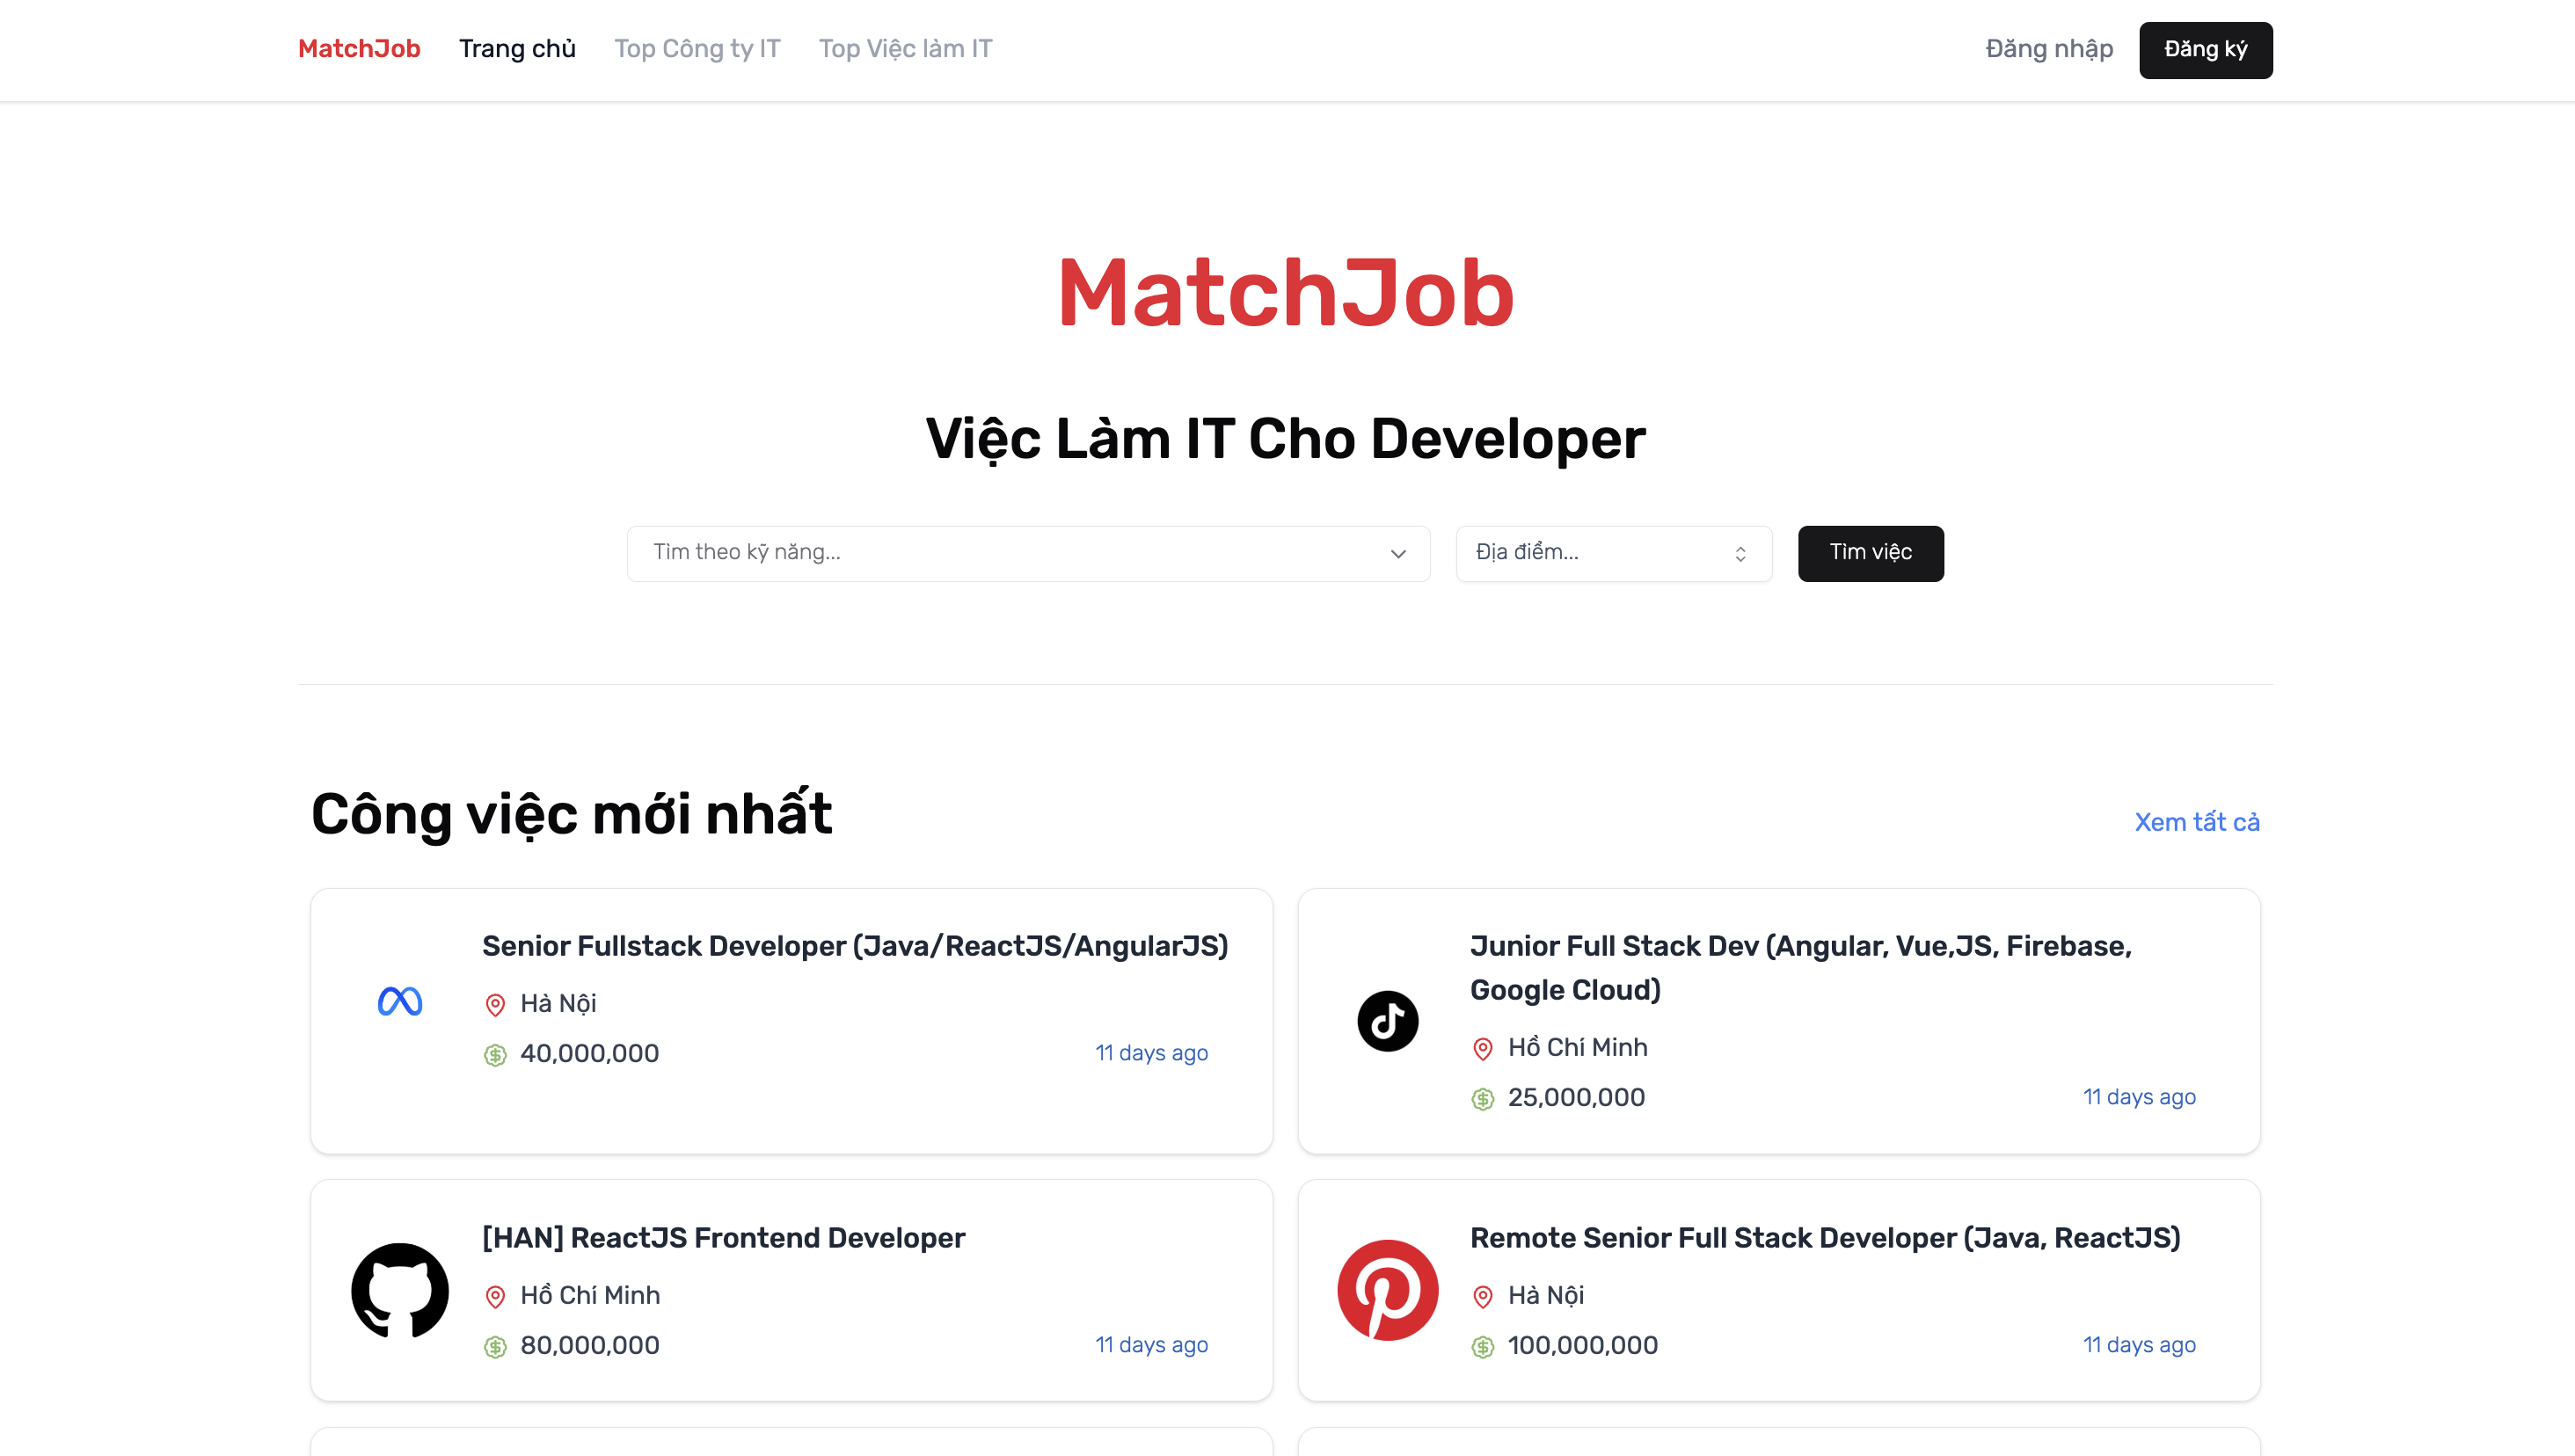
\includegraphics[width=\linewidth]{DBMS-Application/Images/user-screen-job.png}
    \caption{Trang chủ - Danh sách công việc đang tuyển dụng}
    \label{fig:homepage-job}
\end{figure}

Truy vấn sử dụng: \textbf{Query with composite condition}
\begin{lstlisting}
async findAll(current: number, pageSize: number, qs: string) {
    // Loc ra dieu kien filter va sort tu query parameters
    const { filter } = aqp(qs);

    // Truy van: Danh sach cong viec thoa man dieu kien filter
    const jobs = await this.db
      .collection('jobs')
      .find(filter)
      .skip((current - 1) * pageSize)
      .limit(pageSize)
      .toArray();

    // Tra ve response cho Frontend
    return jobs;
}
\end{lstlisting}

Giải thích:

\begin{enumerate}
    \item Frontend sẽ tự động gửi yêu cầu đến Backend thông qua API:
    \begin{lstlisting}[numbers=none]
GET /api/jobs?current=0&pageSize=6
    \end{lstlisting}
    
    \item Backend sẽ nhận được query parameters (\texttt{current} và \texttt{pageSize}) từ Frontend và thực hiện truy vấn CSDL với filter và phân trang:
    \begin{itemize}
        \item Sử dụng \texttt{find()} để lọc dữ liệu theo điều kiện \texttt{filter} (trong trường hợp này, \texttt{filter} là object rỗng (\texttt{\{\}}) nên sẽ trả về tất cả các công việc có trong hệ thống)
        \item Sử dụng \texttt{skip()} để bỏ qua các bản ghi không cần thiết
        \item Sử dụng \texttt{limit()} để giới hạn số lượng bản ghi trả về
    \end{itemize}

    \item Sau khi truy vấn được thực hiện thành công, Backend phản hồi danh sách các công việc cho Frontend để hiển thị lên giao diện người dùng
\end{enumerate}

Người dùng có thể tìm kiếm công việc bằng cách lọc theo \textbf{Địa điểm} và \textbf{Kỹ năng yêu cầu}. Ví dụ, tìm các công việc có yêu cầu kỹ năng \textbf{"React.JS"} và \textbf{"React Native"} tại \textbf{TP. Hồ Chí Minh}, hệ thống sẽ hiện lên một pop-up chứa các công việc thoả mãn.

\begin{figure}[H]
    \centering
    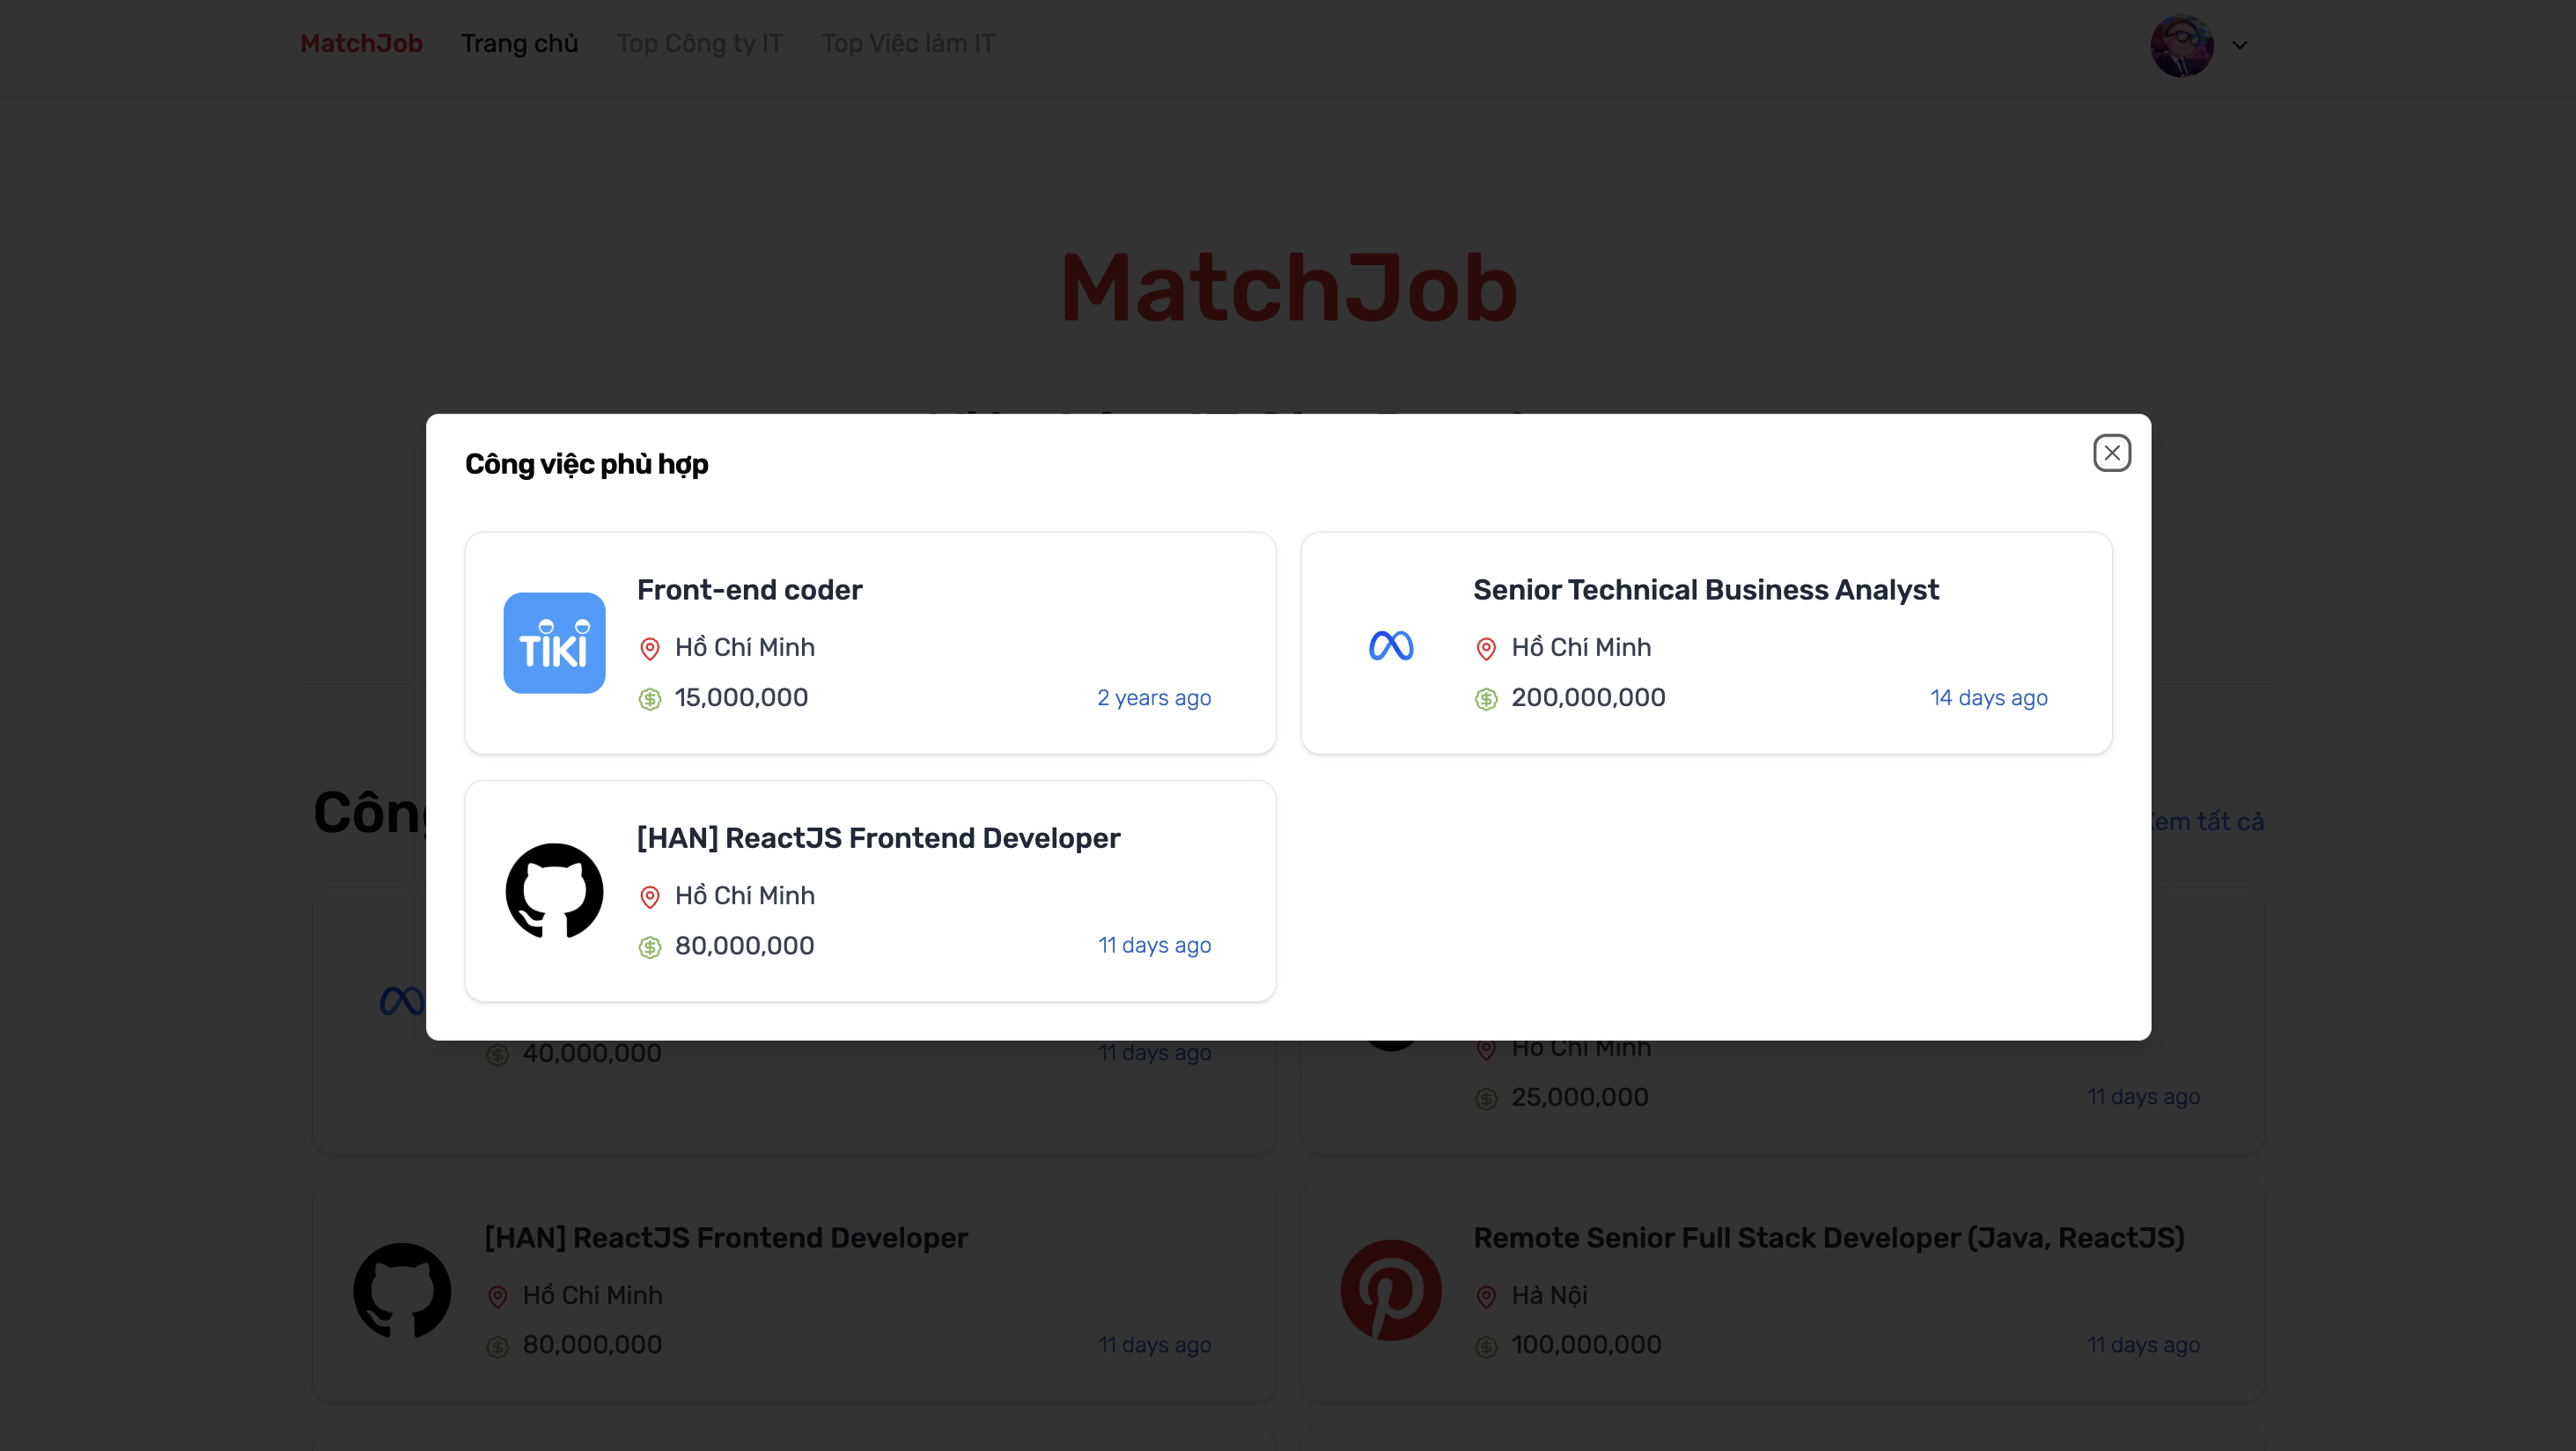
\includegraphics[width=\linewidth]{DBMS-Application/Images/modal-job-search.png}
    \caption{Trang chủ - Lọc công việc theo Địa điểm và Kỹ năng}
    \label{fig:homepage-job-search-filter}
\end{figure}

Truy vấn sử dụng: \textbf{Query with single/composite condition}

\begin{lstlisting}
async getJobsByLocationAndSkills(location: string, skills: string[]) {
    const query: { location?: string; skills?: { $in: string[] } } = {};

    if (location) query.location = location; 
    if (skills.length > 0) query.skills = { $in: skills }; 
    // query = { location: 'HOCHIMINH', skills: { $in: ['REACT.JS', 'REACT NATIVE'] } }

    // Truy van: Loc cac cong viec theo Ky nang va Dia diem
    return await this.db // Truy cap vao database he thong
    .collection('jobs')  // Truy cap vao collection 'jobs'
    .find(query)         // Loc theo dieu kien 'location' va 'skills' trong query
    .toArray();          // Chuyen ket qua ve dang mang
  }
\end{lstlisting}

Giải thích truy vấn:
\begin{itemize}
    \item Back-end nhận được yêu cầu từ Front-end, chứa 2 tham số \texttt{location} và \texttt{skills} trong query parameters và thực hiện xây dựng điều kiện lọc \texttt{query} với các giá trị đó
    
    Ví dụ: \texttt{ query = \{ location : ’HOCHIMINH’, skills : \{ \$in : [ ’REACT.JS’, ’REACT NATIVE’] \} \} }

    \item Sau đó, Back-end sẽ thực hiện truy vấn đến CSDL để lọc ra các công việc thoả mãn điều kiện vừa xây dựng được, và phản hồi về cho Front-end khi thành công
\end{itemize}

Người dùng cũng có thể xem được các công ty tuyển dụng hàng đầu cùng một số thông tin như: tên, logo công ty, số lượng công việc đang tuyển và thu thập cao nhất.

\begin{figure}[H]
    \centering
    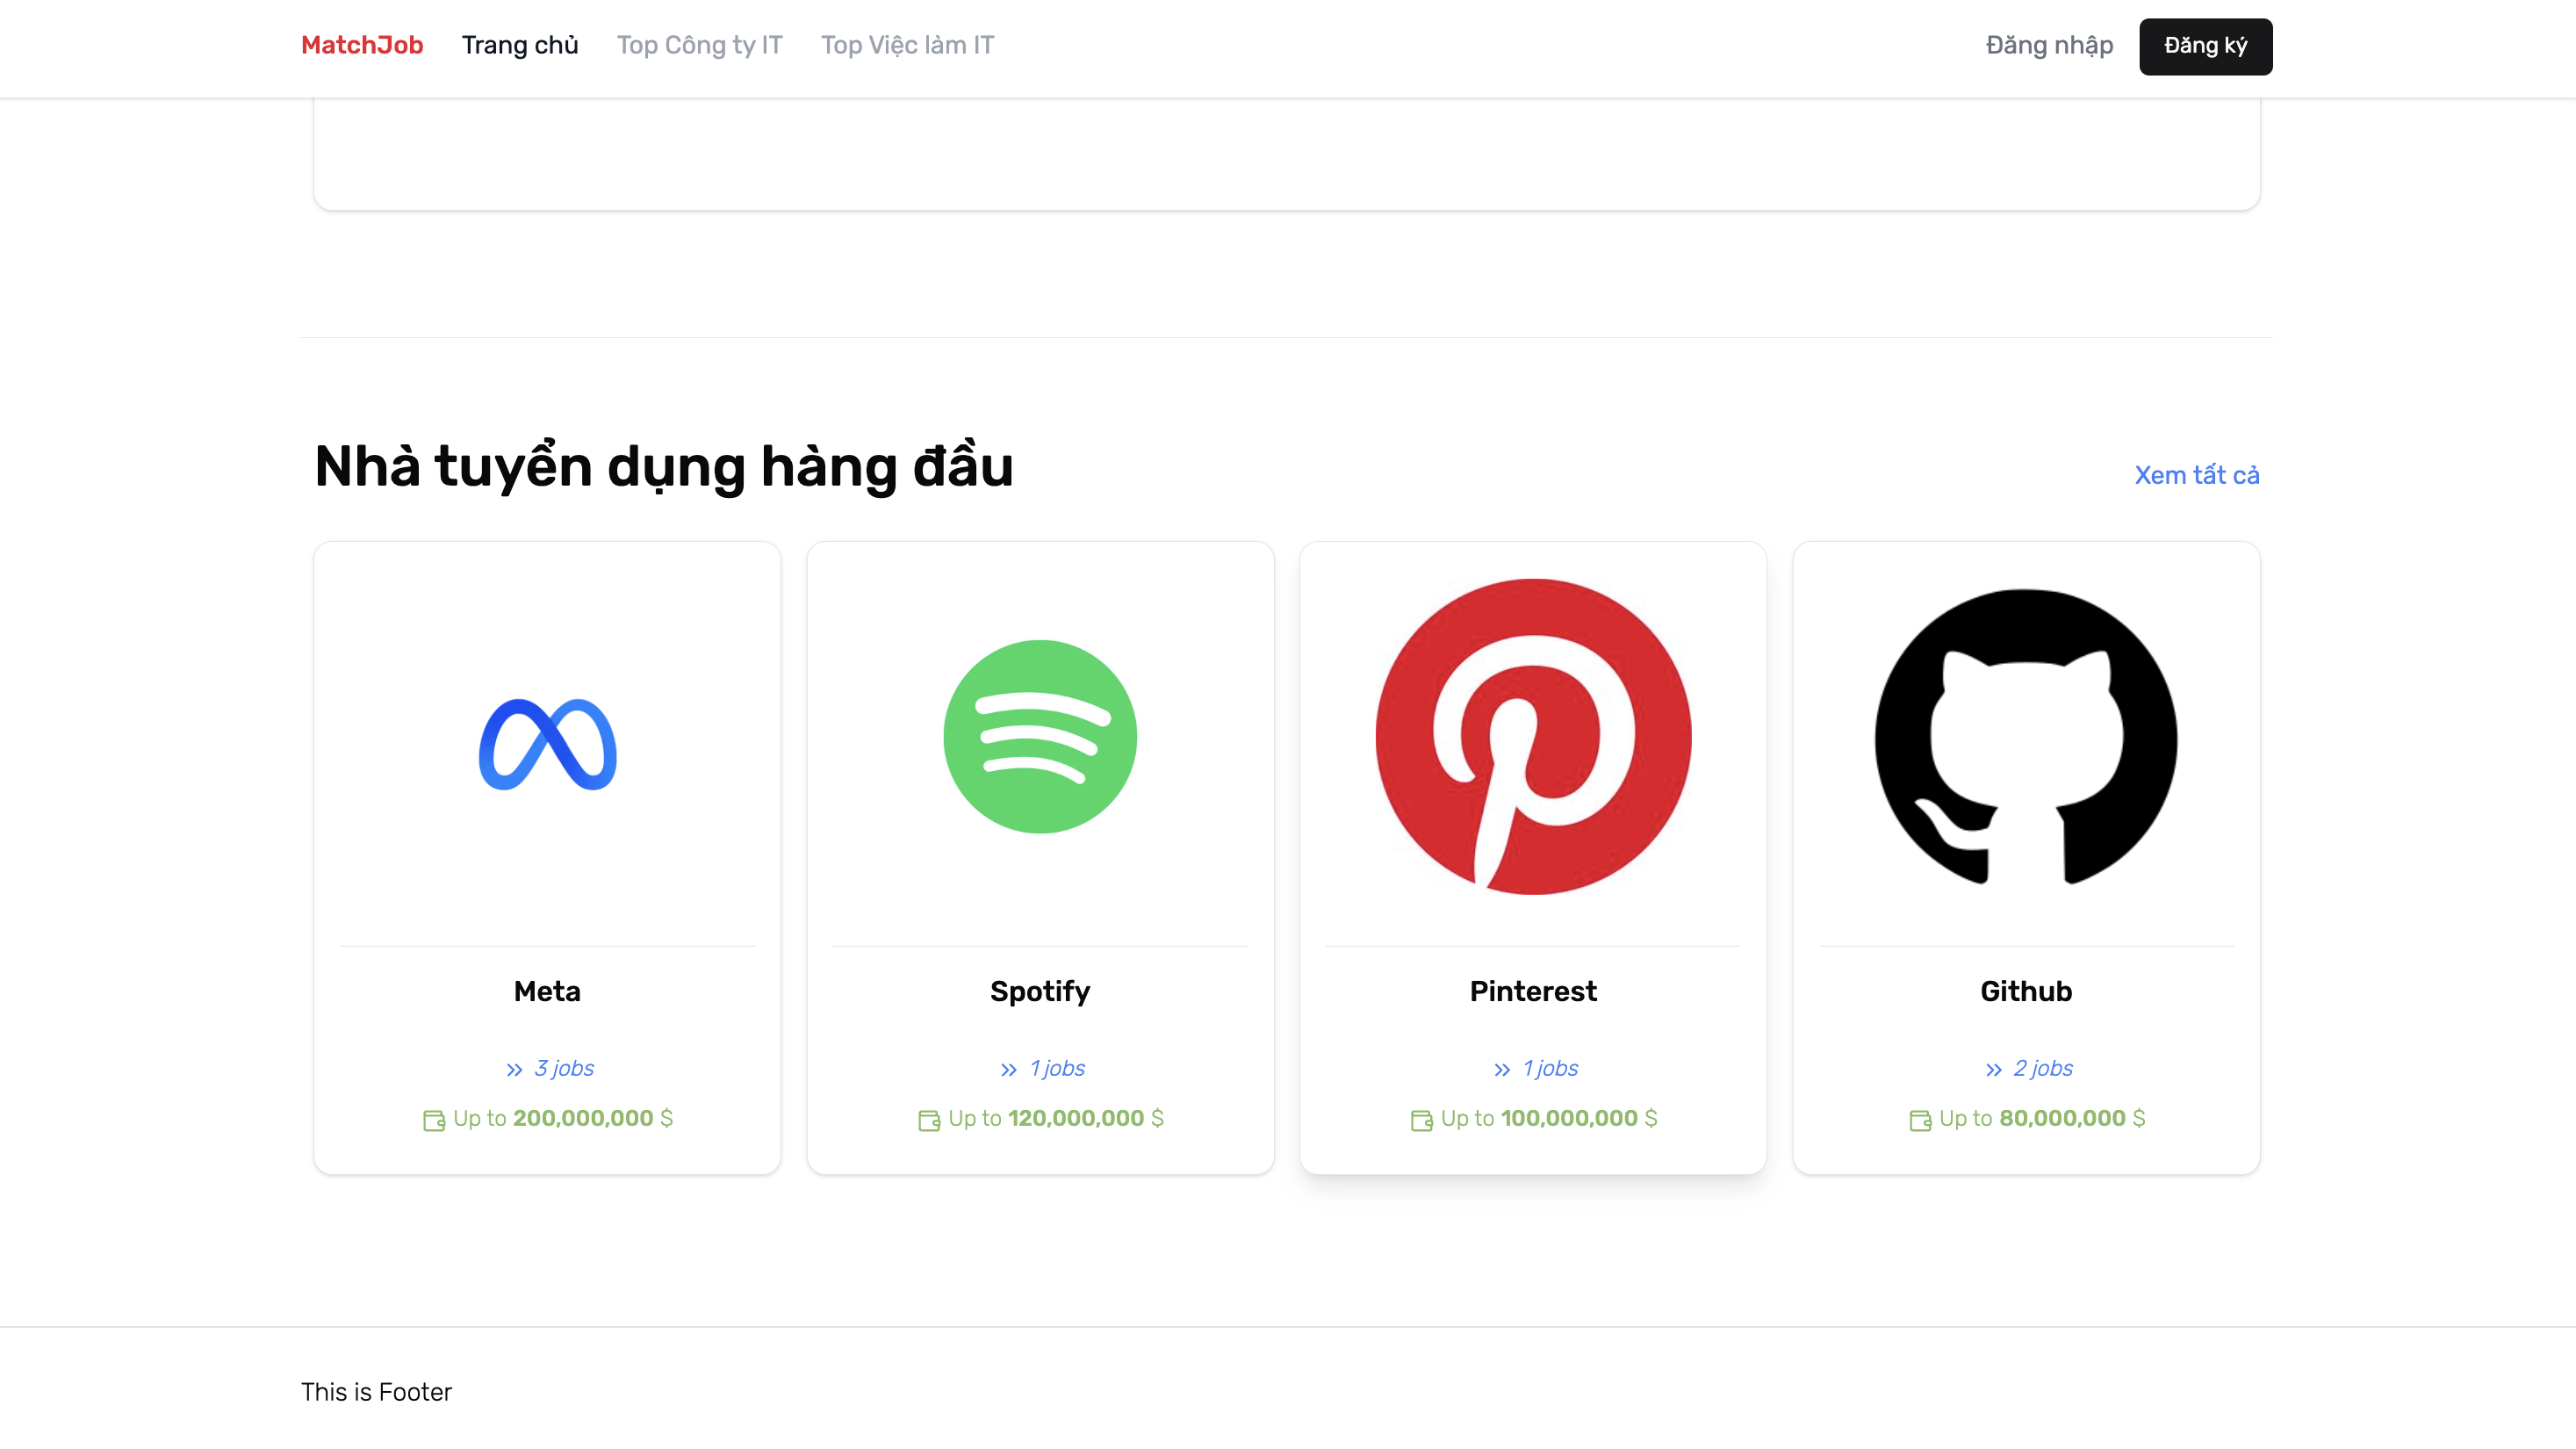
\includegraphics[width=\linewidth]{DBMS-Application/Images/user-screen-company.png}
    \caption{Trang chủ - Danh sách công ty tuyển dụng hàng đầu}
    \label{fig:homepage-company}
\end{figure}

Truy vấn sử dụng:
\begin{itemize}
    \item \textbf{Query with join}: Sử dụng và \texttt{\$lookup} để join collections \textbf{companies} với \textbf{jobs}
    \item \textbf{Query with aggregation functions}: Sử dụng \texttt{\$size}, \texttt{\$max}, \texttt{\$reduce} để tính toán số lượng công việc, mức lương cao nhất của công ty
\end{itemize}

\begin{lstlisting}
const pipeline = [
  { $match: filter },
  {
    $lookup: {
      from: 'jobs',
      let: { companyId: { $toString: '$_id' } },
      pipeline: [
        {
          $match: {
            $expr: {
              $eq: ['$company._id', '$$companyId'],
            },
          },
        },
      ],
      as: 'jobs',
    },
  },
  {
    $project: {
      _id: 1,
      name: 1,
      address: 1,
      description: 1,
      logo: 1,
      totalJobs: { $size: '$jobs' }, // Dem so luong cong viec
      maxSalary: { $max: '$jobs.salary' }, // Lay ra salary cao nhat
      maxSalaryJobId: {
        $reduce: {
          input: '$jobs',
          initialValue: null,
          in: {
            $cond: [
              { $eq: ['$$this.salary', { $max: '$jobs.salary' }] },
              '$$this._id',
              '$$value',
            ],
          },
        },
      },
    },
  },
  { $sort: { maxSalary: -1 } }, // Sap xep cong ty giam dan theo maxSalary
  { $skip: offset },
  { $limit: limit },
];

return await this.db
  .collection('companies')
  .aggregate(pipeline)
  .toArray();
\end{lstlisting}

Giải thích truy vấn: 
\begin{itemize}
    \item \texttt{\$match}: Lọc các công ty thỏa mãn điều kiện.
    \item \texttt{\$lookup}: Join collection \textbf{companies} (\texttt{\_id}) collection \textbf{jobs} (\texttt{companyId}) để lấy các công việc ứng với từng công ty
    \item \texttt{\$project}: Lọc ra các trường trong collection \textbf{companies} như \texttt{\_id}, \texttt{name}, \texttt{address}, \texttt{logo} và Tính toán các thông tin thống kê như số lượng công việc (\texttt{totalJobs}), lương cao nhất (\texttt{maxSalary}) và ID công việc có lương cao nhất (\texttt{maxSalaryJobId}) của từng công ty
    \item \texttt{\$sort}: Sắp xếp các công ty giảm dần theo lương cao nhất (\texttt{maxSalary})
    \item \texttt{\$skip} và \texttt{\$limit}: Phân trang kết quả
\end{itemize}

Bên cạnh đó, người dùng có thể xem nhanh thông tin các công việc đang tuyển dụng của một công ty cụ thể, thông qua các thẻ công ty được hiển thị:

\begin{figure}[H]
    \centering
    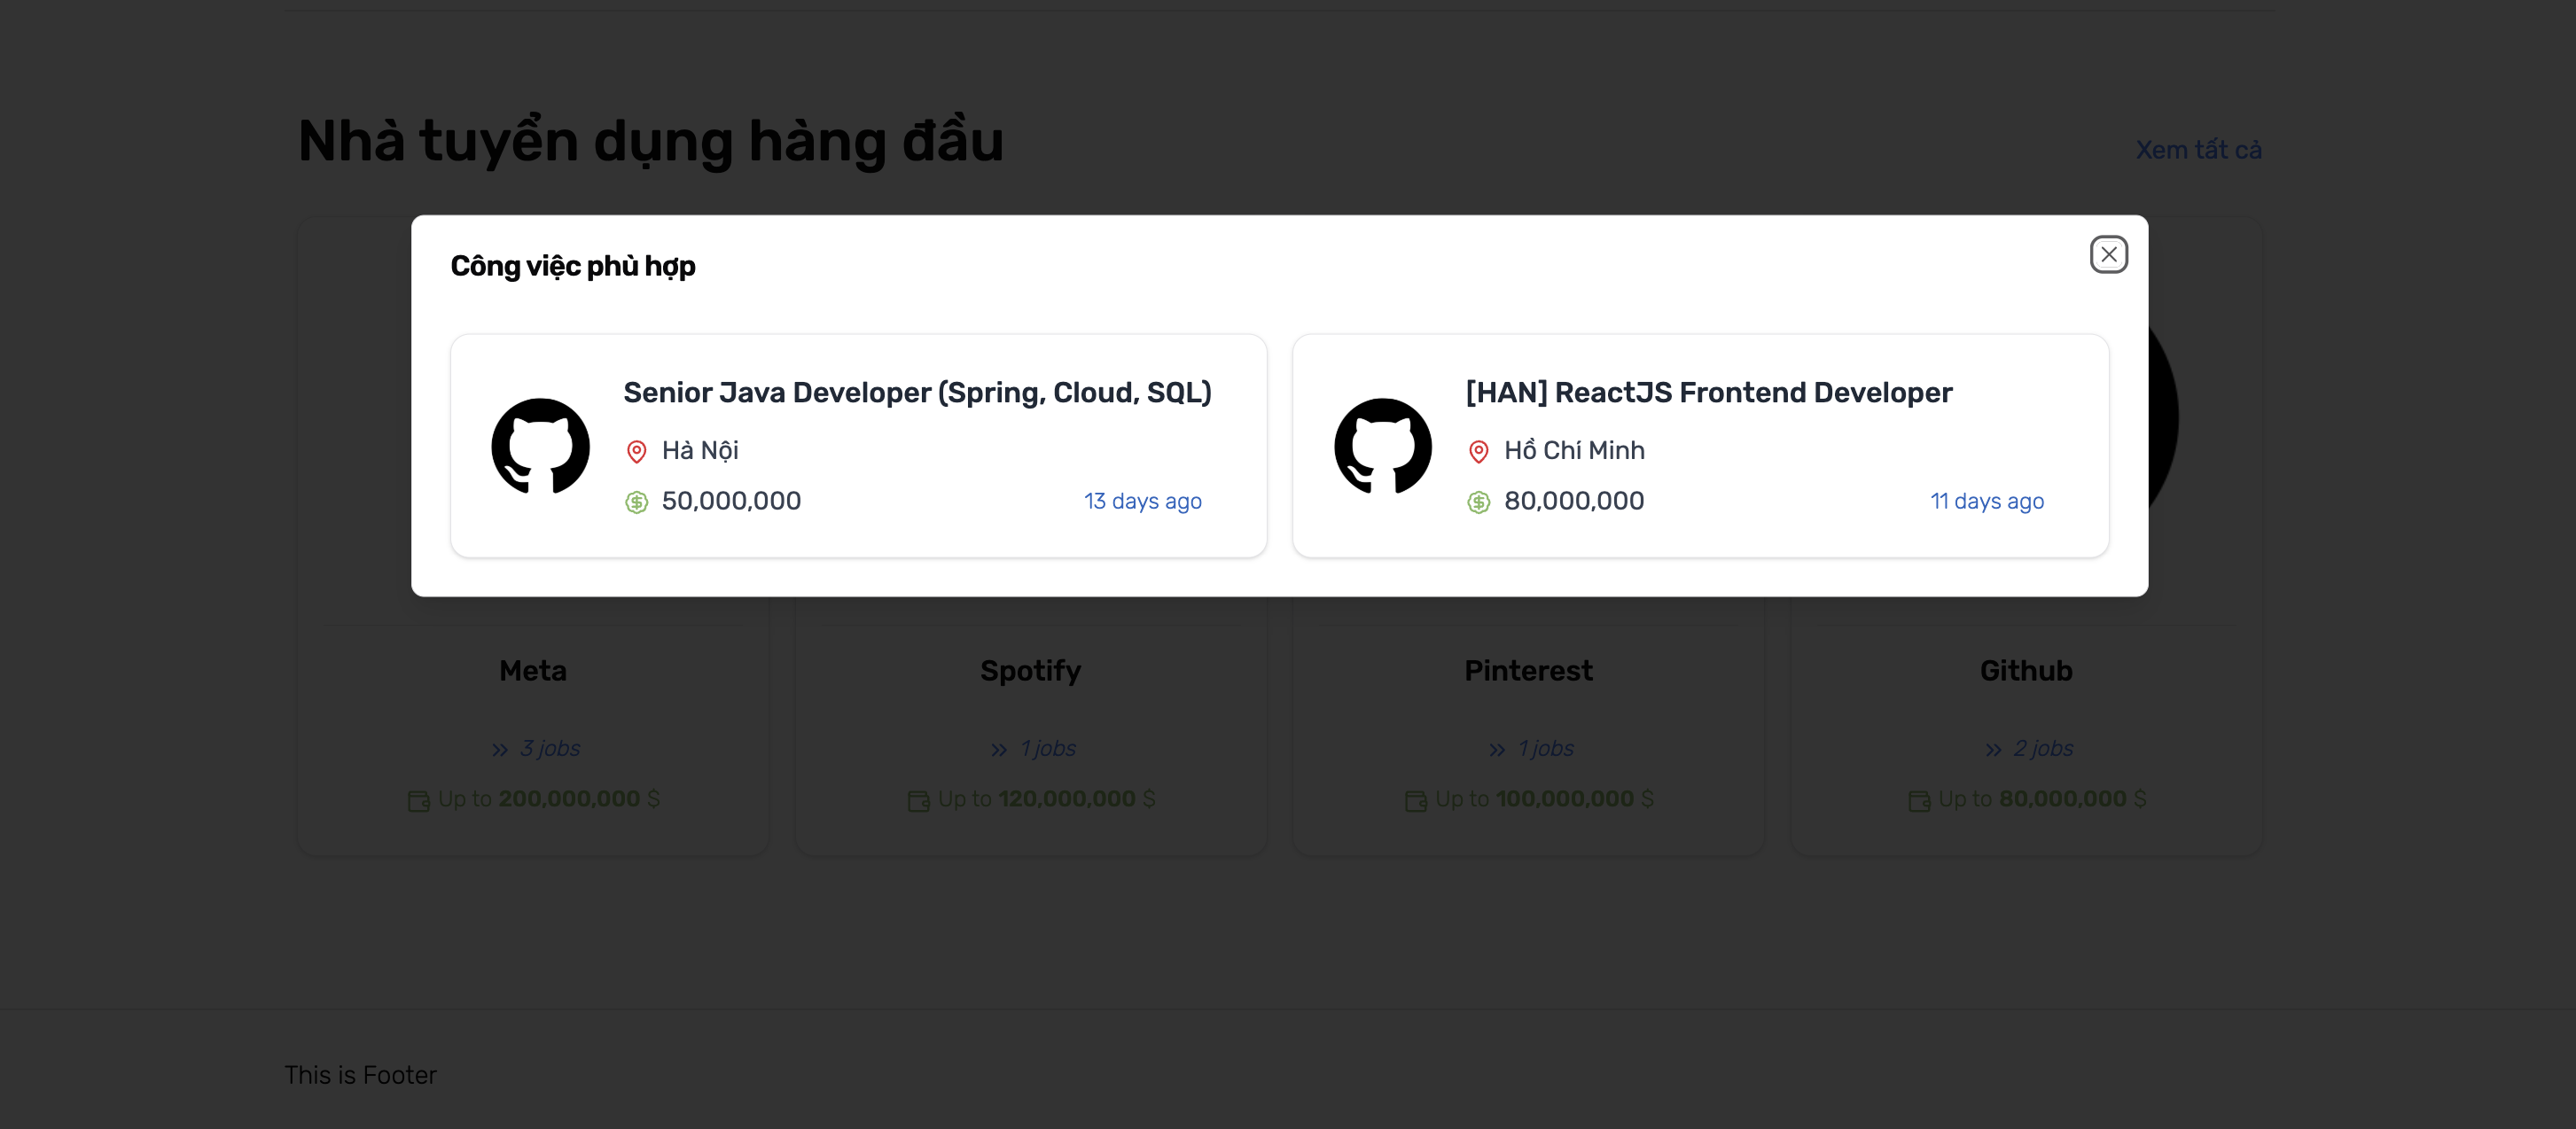
\includegraphics[width=\linewidth]{DBMS-Application/Images/modal-job-company.png}
    \caption{Trang chủ - Lọc ra các công việc thuộc một công ty cụ thể}
    \label{fig:homepage-job-company}
\end{figure}

Truy vấn sử dụng:
\begin{itemize}
    \item \textbf{Query with single condition}: Lọc document cụ thể từ collection \textbf{companies} dựa trên \texttt{\_id}

    \item \textbf{Query with join}: Thực hiện join giữa collection \textbf{companies} và \textbf{jobs} để lấy công việc liên quan
\end{itemize}

\begin{lstlisting}
const pipeline = [
  {
    $match: { _id: new ObjectId(companyId) }, // Loc ra cong ty co _id = companyId duoc truyen vao
  },
  {
    $lookup: {
      from: 'jobs', // Join collection 'companies' voi collection 'jobs'
      let: { companyId: { $toString: '$_id' } },
      pipeline: [
        {
          $match: {
            $expr: { $eq: ['$company._id', '$$companyId'] },
          },
        },
      ],
      as: 'jobs', // Luu ket qua vao field 'jobs' cho tung cong ty
    },
  },
  {
    $project: { // Loc ra cac field can thiet
      _id: 1,
      name: 1,
      address: 1,
      description: 1,
      logo: 1,
      jobs: 1,
    },
  },
];

return await this.db
  .collection('companies')
  .aggregate(pipeline)
  .toArray();
\end{lstlisting}

Giải thích truy vấn:
\begin{itemize}
    \item \texttt{\$match}: Lọc công ty cụ thể từ collection companies dựa trên \texttt{\_id} được truyền vào (\texttt{companyId}).
    
    \item \texttt{\$lookup}: Join collection \textbf{companies} với collection \textbf{jobs} để tìm tất cả các công việc thuộc công ty đó, bằng cách so sánh \texttt{\_id} của công ty trong \textbf{companies} với \texttt{company.\_id} trong \textbf{jobs} và lưu danh sách công việc vào trường \textbf{jobs}.


    \item \texttt{\$project}: Chọn các trường cần trả về gồm \texttt{\_id}, \texttt{name}, \texttt{address}, \texttt{description}, \texttt{logo}, và \texttt{jobs}.
\end{itemize}

Cuối cùng, người dùng có thể xem thống kê các kỹ năng có nhu cầu tuyển dụng nhiều, được thu thập từ các công việc đang được tuyển dụng:

\begin{figure}[H]
    \centering
    \includegraphics[width=\linewidth]{DBMS-Application/Images/user-screen-skill-stats.png}
    \caption{Trang chủ - Thống kê kỹ năng được tuyển dụng nhiều}
    \label{fig:enter-label}
\end{figure}

Truy vấn sử dụng: \textbf{Query with aggregation functions} - Sử dụng \texttt{\$sum} để tính tổng số công việc yêu cầu từng kỹ năng.

\begin{lstlisting}
const pipeline = [
  { $unwind: '$skills' },
  { $group: { _id: '$skills', total: { $sum: 1 } } },
  { $project: { skill: '$_id', total: 1, _id: 0 } },
];

return await this.db
  .collection('jobs')
  .aggregate(pipeline)
  .toArray();
\end{lstlisting}

Giải thích truy vấn:
\begin{itemize}
    \item \texttt{\$unwind}: Tách từng phần tử trong mảng skills của mỗi công việc thành các document riêng lẻ.
    \item \texttt{\$group}: Nhóm các document theo kỹ năng (skills) và đếm số lượng công việc yêu cầu kỹ năng đó bằng cách cộng dồn (\$sum: 1).
    \item \texttt{\$project}: Chọn các trường cần trả về, đổi tên \_id thành skill và bỏ trường \_id trong kết quả.
\end{itemize}
\subsubsection{Giao diện người dùng - Danh sách/Chi tiết công ty}

Khi truy cập vào trang danh sách công ty, Front-end sẽ tự động fetch dữ liệu từ Backend thông qua một API tương tự như ở trang chủ: thực hiện phân trang để lấy lần lượt các công ty trong cơ sở dữ liệu dựa trên tham số \texttt{current} và \texttt{pageSize}.

\begin{figure}[H]
    \centering
    \includegraphics[width=\linewidth]{DBMS-Application/Images/list-company.png}
    \caption{Danh sách công ty}
    \label{fig:enter-label}
\end{figure}

Khi người dùng chọn 1 công ty trong danh sách, Front-end sẽ gửi yêu cầu đến API để lấy thông tin chi tiết của công ty đó và hiển thị lên giao diện người dùng:

\begin{figure}[H]
    \centering
    \includegraphics[width=\linewidth]{DBMS-Application/Images/company-detail.png}
    \caption{Thông tin chi tiết của công ty}
    \label{fig:enter-label}
\end{figure}

Truy vấn sử dụng: \textbf{Query with single condition} - Sử dụng điều kiện \texttt{\_id} để tìm công ty duy nhất

\begin{lstlisting}
return await this.db
  .collection('companies')
  .findOne({ _id: new ObjectId(id) }); // Chuyen id truyen vao thanh ObjectId, phu hop voi MongoDB
\end{lstlisting}

Ngoài ra, người dùng cũng có thể xem các công việc hiện đang được tuyển dụng của công ty này thông qua API lọc ra công việc của một công ty cụ thể (đã trình bày ở phần Trang chủ), hệ thống sẽ hiện lên 1 popup chứa các công việc của công ty hiện tại như sau:

\begin{figure}[H]
    \centering
    \includegraphics[width=\linewidth]{DBMS-Application/Images/modal-job-in-company-detail.png}
    \caption{Các công việc đang tuyển dụng của công ty cụ thể}
    \label{fig:enter-label}
\end{figure}



\subsubsection{Giao diện người dùng - Danh sách/Chi tiết công việc}

Khi truy cập vào trang danh sách công việc tuyển dụng, Front-end sẽ tự động fetch dữ liệu từ Backend thông qua một API tương tự như ở trang chủ: thực hiện phân trang để lấy lần lượt các công việc trong cơ sở dữ liệu dựa trên tham số \texttt{current} và \texttt{pageSize}.

\begin{figure}[H]
    \centering
    \includegraphics[width=\linewidth]{DBMS-Application/Images/list-job.png}
    \caption{Danh sách công việc đang được tuyển dụng}
\end{figure}

Và cũng như ở trang Danh sách công ty đã trình bày, người dùng cũng có thể chọn 1 công việc để xem chi tiết công việc đó:

\begin{figure}[H]
    \centering
    \includegraphics[width=\linewidth]{DBMS-Application/Images/job-detail.png}
    \caption{Danh sách công việc đang được tuyển dụng}
\end{figure}

Truy vấn sử dụng: \textbf{Query with single condition} - Sử dụng điều kiện \texttt{\_id} để tìm công việc duy nhất

\begin{lstlisting}
return await this.db
  .collection('jobs')
  .findOne({ _id: new ObjectId(id) });
\end{lstlisting}

Bên cạnh đó, hệ thống Front-end cũng tự động gửi yêu cầu thông qua API để lấy về số lượng hồ sơ đã nộp từ các ứng viên khác cho công việc hiện tại

\begin{figure}[H]
    \centering
    \includegraphics[width=.75\linewidth]{DBMS-Application/Images/number-resumes-apply.png}
    \caption{Số lượng hồ sơ đã được nộp cho công việc hiện tại}
\end{figure}

Truy vấn sử dụng:
\begin{itemize}
    \item \textbf{Query with single condition}: Sử dụng \texttt{\$match} để tìm một công việc cụ thể trong collection \textbf{jobs} dựa trên \texttt{\_id}
    
    \item \textbf{Query with join}: Thực hiện join thông qua \texttt{\$lookup} giữa collection \textbf{jobs} (\texttt{\_id}) và \textbf{resumes} (\texttt{jobId}) để lấy danh sách hồ sơ ứng tuyển của đến công việc đó

    \item \textbf{Query with aggregation functions}: Sử dụng \texttt{\$size} để tính tổng số lượng hồ sơ ứng tuyển của công việc
\end{itemize}

\begin{lstlisting}
const pipeline = [
  {
    $match: { _id: new ObjectId(id) }, // Tim job cu the thong qua _id
  },
  {
    $lookup: {
      from: 'resumes', // Join collection 'jobs' voi collection 'resumes'
      localField: '_id',
      foreignField: 'jobId',
      as: 'resumes',
    },
  },
  {
    $project: {
      _id: 1,
      totalResumes: { $size: '$resumes' }, // Dem so luong resumes da nop
    },
  },
];

const result = await this.db
  .collection('jobs')
  .aggregate(pipeline)
  .toArray();

return result[0];
\end{lstlisting}

Giải thích truy vấn:
\begin{itemize}
    \item \texttt{\$match}: Lọc công việc cụ thể từ collection \textbf{jobs} dựa trên \_id.
    \item \texttt{\$lookup}: Join với collection \textbf{resumes} để tìm các hồ sơ ứng tuyển có trường \texttt{jobId} trùng với \texttt{\_id} của công việc
    \item \texttt{\$project}: Trả về \texttt{\_id} của công việc và tổng số hồ sơ ứng tuyển (\texttt{totalResumes}) bằng cách sử dụng \texttt{\$size} để đếm số phần tử trong mảng resumes.
\end{itemize}

Cuối cùng, người dùng có thể upload (tạo) hồ sơ và apply cho công việc cụ thể:

\begin{figure}[H]
    \centering
    \includegraphics[width=\linewidth]{DBMS-Application/Images/modal-upload-cv.png}
    \caption{Số lượng hồ sơ đã được nộp cho công việc hiện tại}
\end{figure}

Truy vấn sử dụng: \textbf{Insert}

\begin{lstlisting}
const newResume = {
  url,
  companyId: new ObjectId(companyId),
  email,
  jobId: new ObjectId(jobId),
  userId: new ObjectId(_id),
  status: 'PENDING',
  createdAt: new Date(),
  updatedAt: new Date(),
};

const result = await this.db.collection('resumes').insertOne(newResume); // Them ho so ung tuyen moi vao database

return {
  _id: result.insertedId,
  createdAt: newResume.createdAt,
};

\end{lstlisting}

\subsubsection{Giao diện người dùng - Danh sách hồ sơ đã ứng tuyển}

Người dùng có thể xem lại các hồ sơ ứng tuyển của họ cho từng công việc:

\begin{figure}[H]
    \centering
    \includegraphics[width=\linewidth]{DBMS-Application/Images/modal-list-cv.png}
    \caption{Các hồ sơ đã được nộp của một người dùng}
\end{figure}

Truy vấn sử dụng:
\begin{itemize}
    \item \textbf{Query with join}: Sử dụng \texttt{\$lookup} để liên kết dữ liệu giữa hai collection \textbf{users} và \textbf{resumes}

    \item \textbf{Query with single condition}: Sử dụng \texttt{\$match} để lọc hồ sơ của của người dùng có \texttt{\_id}
\end{itemize}

\begin{lstlisting}
const result = await this.db
  .collection('users')
  .aggregate([
    {
      $lookup: {
        from: 'resumes',
        localField: '_id',
        foreignField: 'userId',
        as: 'userResumes',
      },
    },
    {
      $match: {
        _id: new ObjectId(user._id),
      },
    },
    {
      $project: {
        userResumes: 1,
      },
    },
  ])
  .toArray();

const resumes = result.length > 0 ? result[0].userResumes : [];
return resumes;
\end{lstlisting}

Giải thích truy vấn:
\begin{itemize}
    \item \texttt{\$lookup}: Thực hiện join giữa collection \textbf{users} và collection \textbf{resumes} để lấy tất cả các hồ sơ ứng tuyển của người dùng (\texttt{userId}) tương ứng với \texttt{\_id} của user.
    \item \texttt{\$match}: Lọc để chỉ lấy hồ sơ ứng tuyển của người dùng có \texttt{\_id} trùng với ID của user được truyền vào (\texttt{user.\_id}).
    \item \texttt{\$project}: Chỉ giữ lại trường \texttt{userResumes} trong kết quả trả về, ẩn các trường khác.
\end{itemize}

Truy vấn trả về mảng các hồ sơ ứng tuyển (\texttt{userResumes}) của người dùng (trả về mảng rỗng trong trường hợp người dùng chưa tải lên hồ sơ ứng tuyển nào)
\subsubsection{Giao diện Admin - Quản lý công việc}

Trang quản lý công việc được thiết kế để hiển thị danh sách toàn bộ các công việc hiện có trong hệ thống, phục vụ việc quản lý, chỉnh sửa hoặc xóa công việc. Dữ liệu cũng được lấy từ Backend thông qua API theo cơ chế phân trang tương tự như các phần trước, giúp tối ưu hóa hiệu suất và hiển thị mượt mà, đặc biệt khi số lượng công việc lớn.

\begin{figure}[H]
    \centering
    \includegraphics[width=\linewidth]{DBMS-Application/Images/admin-job.png}
    \caption{Trang quản lý công việc - Danh sách các công việc trong hệ thống}
    \label{fig:enter-label}
\end{figure}

Quản trị viên cũng có thể tìm kiếm và lọc ra các công ty theo \textbf{Tên}, \textbf{Mức lương} và \textbf{Level} như sau:

\begin{figure}[H]
    \centering
    \includegraphics[width=\linewidth]{DBMS-Application/Images/admin-job-filter.png}
    \caption{Trang quản lý công việc - Danh sách công việc lọc theo điều kiện}
    \label{fig:enter-label}
\end{figure}

Truy vấn sử dụng: \textbf{Query with single/composite condition}\\

Bên cạnh đó, quản trị viên cũng có thể thêm công việc mới, bằng cách điền các thông tin cần thiết vào giao diện dưới đây. Sau đó, hệ thống sẽ gửi thông tin này đến cơ sở dữ liệu để thực hiện việc thêm document mới vào collection \textbf{jobs}.

\begin{figure}[H]
    \centering
    \includegraphics[width=\linewidth]{DBMS-Application/Images/create-job.png}
    \caption{Trang quản lý công việc - Thêm công việc mới}
    \label{fig:enter-label}
\end{figure}

Truy vấn sử dụng: \textbf{Insert}

\begin{lstlisting}
async create(createJobDto: CreateJobDto) {
    const job = {
      ...createJobDto,
      createdAt: new Date(),
      updatedAt: new Date(),
    };

    const result = await this.db.collection('jobs').insertOne(job); // Insert cong viec moi vao collection 'jobs'
    return { _id: result.insertedId, createdAt: job.createdAt };
}
\end{lstlisting}

Quản trị viên cũng có thể chọn một công việc để chỉnh sửa/cập nhật thông tin. Khi đó, dựa vào \texttt{\_id}, hệ thống sẽ truy vấn cơ sở dữ liệu để lấy ra công việc đó (\textbf{query with single condition}) và hiển thị lên giao diện. Lúc này, quản trị viên có thể tiến hành sửa lại các thông tin đó và khi hoàn tất, Front-end sẽ gửi yêu cầu qua API với phương thức HTTP \textbf{PATCH} để hệ thống tiến hành cập nhật lại thông tin cho công việc đó trong cơ sở dữ liệu.

\begin{figure}[H]
    \centering
    \includegraphics[width=\linewidth]{DBMS-Application/Images/update-job.png}
    \caption{Trang quản lý công việc - Cập nhật thông tin cho một công việc cụ thể}
    \label{fig:enter-label}
\end{figure}

Truy vấn sử dụng: \textbf{Update}

\begin{lstlisting}
const result = await this.db.collection('jobs').updateOne(
  { _id: new ObjectId(id) },
  {
    $set: {
      ...updateJobDto,
      updatedAt: new Date(),
    },
  },
);
\end{lstlisting}

Cuối cùng, quản trị viên có thể chọn một công việc để xoá khỏi hệ thống. Khi đó, một popup sẽ hiện lên để xác nhận với quản trị viên về việc xoá công ty đã chọn ra khỏi cơ sở dữ liệu

\begin{figure}[H]
    \centering
    \includegraphics[width=\linewidth]{DBMS-Application/Images/delete-job.png}
    \caption{Trang quản lý công việc - Xác nhận xoá công việc chỉ định khỏi hệ thống}
    \label{fig:enter-label}
\end{figure}

Khi quản trị viên xác nhận, Back-end gửi truy vấn đến cơ sở dữ liệu để tìm theo \texttt{\_id} và xoá công việc đó ra khỏi cơ sở dữ liệu. Khi đó, giao diện người dùng sẽ được cập nhật lại.\\

\begin{figure}[H]
    \centering
    \includegraphics[width=\linewidth]{DBMS-Application/Images/delete-job-successfully.png}
    \caption{Trang quản lý công việc - Xoá thành công công việc đã chọn}
    \label{fig:enter-label}
\end{figure}

Truy vấn sử dụng: \textbf{Delete}

\begin{lstlisting}
const result = await this.db
      .collection('jobs')
      .deleteOne({ _id: new ObjectId(id) });
\end{lstlisting}
\subsubsection{Giao diện Admin - Quản lý công ty}

Tương tự trang quản lý công việc, trang quản lý công ty cũng sử dụng các loại truy vấn sau để hỗ trợ cho các thao tác CRUD:
\begin{itemize}
    \item \textbf{Query with single/composite condition}: Để fetch lên dữ liệu toàn bộ công ty trong hệ thống theo cơ chế phân trang và một số điều kiện như \textbf{Tên công ty}, \textbf{Địa chỉ}
    \begin{figure}[H]
        \centering
        \includegraphics[width=\linewidth]{DBMS-Application/Images/admin-company.png}
        \caption{Trang quản lý công ty - Danh sách các công ty trong hệ thống}
        \label{fig:enter-label}
    \end{figure}

    \begin{figure}[H]
        \centering
        \includegraphics[width=\linewidth]{DBMS-Application/Images/admin-company-filter.png}
        \caption{Trang quản lý công ty - Danh sách công ty lọc theo điều kiện}
        \label{fig:enter-label}
    \end{figure}
    
    \item \textbf{Insert}: Thêm mới một công ty
    \begin{figure}[H]
        \centering
        \includegraphics[width=\linewidth]{DBMS-Application/Images/create-company.png}
        \caption{Trang quản lý công ty - Thêm mới công ty}
        \label{fig:enter-label}
    \end{figure}

    \item \textbf{Update}: Cập nhật/chỉnh sửa thông tin công ty cụ thể
    \begin{figure}[H]
        \centering
        \includegraphics[width=\linewidth]{DBMS-Application/Images/update-company.png}
        \caption{Trang quản lý công ty - Cập nhật thông tin công ty}
        \label{fig:enter-label}
    \end{figure}

    \item \textbf{Delete}: Xoá công ty cụ thể
    \begin{figure}[H]
        \centering
        \includegraphics[width=\linewidth]{DBMS-Application/Images/delete-company.png}
        \caption{Trang quản lý công ty - Xoá công ty}
        \label{fig:enter-label}
    \end{figure}
\end{itemize}
\subsubsection{Giao diện Admin - Quản lý người dùng}

Tương tự với trang quản lý công ty và quản lý công việc, trang quản lý người dùng cũng sử dụng các loại truy vấn sau để hỗ trợ cho các thao tác CRUD:

\begin{itemize}
    \item \textbf{Query with single/composite condition}: Để fetch lên dữ liệu toàn bộ người dùng trong hệ thống theo cơ chế phân trang và một số điều kiện như \textbf{Tên người dùng}, \textbf{Email}
    \begin{figure}[H]
        \centering
        \includegraphics[width=\linewidth]{DBMS-Application/Images/admin-user.png}
        \caption{Trang quản lý người dùng - Danh sách người dùng trong hệ thống}
        \label{fig:enter-label}
    \end{figure}
    
    \item \textbf{Insert}: Thêm mới một người dùng
    \begin{figure}[H]
        \centering
        \includegraphics[width=\linewidth]{DBMS-Application/Images/create-user.png}
        \caption{Trang quản lý người dùng - Thêm mới người dùng}
        \label{fig:enter-label}
    \end{figure}

    \item \textbf{Update}: Cập nhật/chỉnh sửa thông tin người dùng cụ thể
    \begin{figure}[H]
        \centering
        \includegraphics[width=\linewidth]{DBMS-Application/Images/update-user.png}
        \caption{Trang quản lý người dùng - Cập nhật thông tin người dùng}
        \label{fig:enter-label}
    \end{figure}

    \item \textbf{Delete}: Xoá người dùng
    \begin{figure}[H]
        \centering
        \includegraphics[width=\linewidth]{DBMS-Application/Images/delete-user.png}
        \caption{Trang quản lý người dùng - Xoá người dùng}
        \label{fig:enter-label}
    \end{figure}
\end{itemize}
\subsubsection{Giao diện Admin - Quản lý hồ sơ ứng tuyển}

\begin{itemize}
    \item \textbf{Query with composite condition}: Để fetch lên dữ liệu toàn bộ hồ sơ ứng tuyển trong hệ thống theo cơ chế phân trang
    \begin{figure}[H]
        \centering
        \includegraphics[width=\linewidth]{DBMS-Application/Images/admin-resume.png}
        \caption{Trang quản lý hồ sơ ứng tuyển - Danh sách hồ sơ ứng tuyển trong hệ thống}
        \label{fig:enter-label}
    \end{figure}

    \item \textbf{Update}: Cập nhật thông tin của hồ sơ ứng tuyển, cụ thể là cập nhật \textbf{trạng thái}
    \begin{figure}[H]
        \centering
        \includegraphics[width=.5\linewidth]{DBMS-Application/Images/update-status-resume.png}
        \caption{Trang quản lý hồ sơ ứng tuyển - Chọn trạng thái mới cho hồ sơ}
        \label{fig:enter-label}
    \end{figure}

    \begin{figure}[H]
        \centering
        \includegraphics[width=\linewidth]{DBMS-Application/Images/update-resume-successfully.png}
        \caption{Trang quản lý hồ sơ ứng tuyển - Cập nhật trạng thái của hồ sơ ứng tuyển thành công}
        \label{fig:enter-label}
    \end{figure}
    
    \item \textbf{Delete}: Xoá hồ sơ ứng tuyển chỉ định
    \begin{figure}[H]
        \centering
        \includegraphics[width=\linewidth]{DBMS-Application/Images/delete-resume.png}
        \caption{Trang quản lý hồ sơ ứng tuyển - Xoá hồ sơ ứng tuyển}
        \label{fig:enter-label}
    \end{figure}
\end{itemize}
\subsection{Kết luận}
Hệ thống đã được hiện thực đầy đủ các yêu cầu chức năng đặt ra, cũng như là các loại truy vấn phức tạp như query with a single condition, query with a composite condition, query with a join, và query with aggregation functions đều đã được áp dụng linh hoạt để xử lý dữ liệu một cách hiệu quả. Tuy nhiên, chỉ riêng query with a subquery không được sử dụng, vì MongoDB không hỗ trợ subquery theo cách truyền thống mà thay vào đó, sử dụng Aggregation Pipeline và các giai đoạn như \$lookup, \$group, và \$match để đạt được kết quả tương đương. Điều này là do MongoDB được thiết kế để xử lý dữ liệu theo hướng document và pipeline thay vì subquery dạng lồng như SQL.

Ngoài ra, giao diện người dùng của hệ thống được thiết kế thông minh, tối giản và dễ sử dụng, tập trung vào việc tối ưu trải nghiệm người dùng. Các thao tác như tìm kiếm, lọc, phân trang, và quản lý dữ liệu được tích hợp mượt mà, giúp hệ thống không chỉ mạnh mẽ về mặt chức năng mà còn thân thiện với người dùng.


\newpage
% \section{Ứng dụng việc làm}

\input{DBMS-Application/2.1.intro}

\input{DBMS-Application/2.2.func-reqs}

\input{DBMS-Application/2.3.data-reqs}

\input{DBMS-Application/2.4.architecture}

\input{DBMS-Application/2.5.implementation}

\input{DBMS-Application/2.6.conclusion}

\section{KẾT LUẬN}
\indent Sau quá trình nghiên cứu và thực hiện đề tài, nhóm đã hoàn thành các mục tiêu đề ra và đạt được kết quả mong muốn. Thông qua việc tìm hiểu các khía cạnh quan trọng của hệ quản trị cơ sở dữ liệu (DBMS) như lưu trữ và quản lý dữ liệu, chỉ mục hóa, xử lý truy vấn, giao dịch, kiểm soát đồng thời, và sao lưu \& khôi phục dữ liệu, nhóm đã phân tích và so sánh chi tiết giữa hai hệ thống PostgreSQL và MongoDB. Kết quả nghiên cứu cho thấy PostgreSQL nổi bật với khả năng xử lý dữ liệu quan hệ phức tạp nhờ kiến trúc mạnh mẽ và hỗ trợ tốt các tiêu chuẩn SQL, trong khi MongoDB, với kiến trúc NoSQL, thể hiện sự linh hoạt và hiệu quả vượt trội khi làm việc với dữ liệu phi cấu trúc hoặc có khối lượng lớn. Trên cơ sở đánh giá ưu nhược điểm của hai hệ thống trên, nhóm đã lựa chọn MongoDB để phát triển ứng dụng Việc làm, một ứng dụng nhắm đến việc quản lý và tìm kiếm thông tin việc làm với yêu cầu xử lý dữ liệu linh hoạt và khả năng mở rộng cao. Ứng dụng đã được triển khai thành công, tận dụng ưu điểm của MongoDB trong việc lưu trữ và xử lý dữ liệu không có cấu trúc, đồng thời đảm bảo hiệu năng cao khi làm việc với khối lượng dữ liệu lớn.u. Qua đề tài này, nhóm không chỉ củng cố kiến thức về các hệ quản trị cơ sở dữ liệu mà còn nắm bắt được quy trình thiết kế và phát triển một ứng dụng thực tế, từ đó rút ra nhiều kinh nghiệm quý báu trong việc chọn lựa và áp dụng công nghệ phù hợp với yêu cầu cụ thể.
%%%%%%%%%%%%%%%%%%%%%%%%%%%%%%%%%
\newpage
\section{TÀI LIỆU THAM KHẢO}
\begin{enumerate}
    \item  R. Elmasri, S. R. Navathe, \textit{Fundamentals of Database Systems}, 7th Edition, Pearson- Addison Wesley, 2016.
    \item \textit{What is Database Management?}, Truy cập ngày 19/12/2024, từ \url{https://www.mongodb.com/resources/basics/databases/database-management}
    \item \textit{Comparing MongoDB vs PostgreSQL}, Truy cập ngày 19/12/2024, từ \url{https://www.mongodb.com/resources/compare/mongodb-postgresql}
    \item \textit{PostgreSQL 17 Documentation}, Truy cập ngày 19/12/2024, từ \url{https://www.postgresql.org/docs/current/storage.html}
    \item \textit{MongoDB Documents}, Truy cập ngày 19/12/2024, từ \url{https://www.mongodb.com/docs/manual/core/document/}
    \item \textit{Advanced Features}, Truy cập ngày 19/12/2024, từ \url{https://www.postgresql.org/docs/current/tutorial-transactions.html}
    \item \textit{Concurrency Control}, Truy cập ngày 19/12/2024, từ
    \url{https://www.postgresql.org/docs/current/mvcc.html}
    \item \textit{Backup and Restore}, Truy cập ngày 19/12/2024, từ \url{https://www.postgresql.org/docs/8.1/backup.html}
    \item \textit{Transactions}, Truy cập ngày 19/12/2024, từ \url{https://www.mongodb.com/docs/manual/core/transactions/}
    \item \textit{FAQ: Concurrency}, Truy cập ngày 19/12/2024, từ \url{https://www.mongodb.com/docs/manual/faq/concurrency/}
    \item \textit{Glossary}, Truy cập ngày 19/12/2024, từ \url{https://www.mongodb.com/docs/manual/reference/glossary/#std-term-concurrency-control}
    \item \textit{Backup Methods for a Self-Managed Deployment}, Truy cập ngày 19/12/2024, từ \url{https://www.mongodb.com/docs/manual/core/backups/}
\end{enumerate}
\end{document}

